\documentclass[oneside,11pt,times]{book}
\usepackage[numbers,sort&compress]{natbib}
%\usepackage{natbib}
\usepackage[margin=1in]{geometry}
\usepackage{rotating}
\usepackage{hyperref}
\usepackage{amssymb}
\usepackage{multirow}
\usepackage{amsmath}
\usepackage{subfigure}
\usepackage{graphicx}
\usepackage[Sonny]{fncychap}
\usepackage{fancyhdr}
\usepackage{bm}
\usepackage{url}
\usepackage{algorithm}
\usepackage{fancybox}
\usepackage{fancyhdr}
\usepackage{listings}
\usepackage{enumitem}
\usepackage[table]{xcolor}
%\usepackage{minipage}
\usepackage{caption}
%\usepackage{subcaption}
\usepackage{pdfpages}
\usepackage{comment}
 \newcommand\omicron{o}

\usepackage{float}
\usepackage[export]{adjustbox}
\usepackage{indentfirst}
\usepackage{amsfonts}
\usepackage{mathrsfs}
\usepackage{array}
\usepackage{listings}
\lstset{
  basicstyle=\ttfamily,
  columns=fullflexible,
  frame=single,
  breaklines=true,
  postbreak=\mbox{\textcolor{red}{$\hookrightarrow$}\space},
}

\usepackage{xcolor}

% TIKZ library for figures
\usepackage{tikz}
\usetikzlibrary{shapes.geometric, arrows}
\tikzstyle{block} = [rectangle, minimum width=3cm, minimum height=0.5cm, text centered, draw=black, fill=white!30]
\tikzstyle{block2} = [rectangle, minimum width=3cm, text width=6.5cm, minimum height=0.5cm, text centered, draw=black, fill=white!30]
\tikzstyle{block3} = [rectangle, minimum width=3cm, text width=4.5cm, minimum height=0.5cm, text centered, draw=black, fill=white!30]
\tikzstyle{choix} = [diamond, minimum width=3cm, minimum height=0.5cm, text centered, draw=black, fill=white!30]
\tikzstyle{choix2} = [diamond, minimum width=3cm, text width=4cm, minimum height=0.5cm, text centered, draw=black, fill=white!30]
\tikzstyle{arrow} = [thick,->,>=stealth]
\tikzstyle{terminus} = [rectangle, rounded corners, minimum width=2.5cm, minimum height=0.5cm,text centered, draw=black, fill=white!30]
\usepackage{pgfplots}
\usepackage{pgfplotstable}
\pgfplotsset{width=10cm,compat=1.9}
\definecolor{dkgreen}{rgb}{0,0.6,0}
\definecolor{gray}{rgb}{0.5,0.5,0.5}
\definecolor{mauve}{rgb}{0.58,0,0.82}

\pagestyle{fancy}
\usepackage{algpseudocode}
\setcounter{secnumdepth}{4}
\setcounter{tocdepth}{4}
\usepackage{color}
\title{\Large{\textbf{MuPhiSim:} a platform for multiphysics simulation\\[10mm] Reference Manual for Users and Developers\\[6mm]}
\author{
%%
}
\date{\today}
}

\begin{document}

\maketitle

%\chapter*{Overview}
%This manual describes \textit{MuPhiSim}: a program to couple finite element and meshless methods, particularly focused on modelling biological tissues. For the former, traditional techniques are used (e.g., type of elements, integration points). For the latter, \textit{max-ent} shape functions are used with the corresponding integration cells. The coupling between them is naturally obtained by exploiting the Kronecker delta property of the \textit{max-ent} and FEM shape functions. \textit{MuPhiSim} solves the equilibrium equations in the total Lagrangian approach. It is programmed in C++ and thus the addition of new capabilities to the program is straightforward, thanks to the inheritance and the abstract classes with their corresponding virtual functions. An input file (.inp) should be provided to the program following the guidelines detailed in this manual. The outputs will be saved to the output folder and viewed with Paraview. The program has been designed to encapsulate all possible improvements within their corresponding folders (e.g., new elements within spatialDiscretisation folder). It should be highlighted that \textit{MuPhiSim} implies a change of paradigm: the simulations are not element oriented, but GPs oriented. So, all loops in the program are over the GPs and not on any element.

%This manual details how to use \textit{MuPhiSim}; how to design an input file with a examples and how to see output results in Paraview. The last chapters contain descriptions of MuPhiSim's developers which worked on different parts of the software such as the spatial and temporal discretisation, the mathematical modelling or how multi-physics is implemented within the mechanical model.

\tableofcontents

%%%%%%%%%%%%%%%%%%%%%%%%%%%%%%%%%%%%%%%% CHAPTER 1 %%%%%%%%%%%%%%%%%%%%%%%%%%%%%%%%%%%%%%%%%%%%
\chapter{USER'S MANUAL}
\begin{center}
    \Large
    \textbf{\textit{User's Reference Manual to understand the main lines of MuPhiSim }}
\end{center}

\section{Introduction}

Meshless methods have attracted the computational mechanics community as a consequence of their adaptability and versatility. These methods are based on a set of nodes without any, a priori, relation between them discretising the problem domain. This is contrary to the finite element method (FEM) in which  nodes are related to each other to build elements. Meshless methods (MM) appear ideal for modelling problems in which the domain suffers large deformations, moving boundaries or material growth. However, these approaches are computationally more expensive than FEM, and the imposition of Dirichlet boundary conditions is more difficult, thus highlighting the coupling between FEM and mesh-free approaches as the best solution.

For installation,  compilation, and execution of the code, please refer to README.txt in the root folder for more information.

\section{Run in Terminal}
It is noted that MuPhiSim can be executed in an arbitrary folder. One can add the path to directory MuPhiSim-dir/bin in \$PATH variable of the system in order to make MuPhiSim executable (\emph{MuPhiSim}) available everywhere by adding the following line in \emph{.bashrc}
\begin{lstlisting}
	export PATH=path-to-MuPhiSim-dir/bin:$PATH
\end{lstlisting}
To run MuPhiSim
\begin{itemize}
	\item in the working folder when TYPE=SEQUENTIAL:
	\begin{lstlisting}
		MuPhiSim-executable -input example.inp
	\end{lstlisting}
	\item in the working folder folder when TYPE=PARALLEL, e.g. run with 3 processors:
	\begin{lstlisting}
		mpiexec -np 3 MuPhiSim-executable -input example.inp
	\end{lstlisting}
\end{itemize}
It is noted that by default, \emph{MuPhiSim} uses two sub-folders respectively named as \emph{input} and \emph{output} to store the input file and the all output files. Other locations can be considered by using the following options
\begin{lstlisting}
	-inputDir indir -outputDir outDir
\end{lstlisting}
where \textit{inDir} and \textit{outDir} are user-defined. 

There are others options can be provided from commandline:
\begin{itemize}
	\item \emph{-MMScalingFactor value} to set the meshless scaling factor by a double specified by \emph{value} [by default: 1]
	\item \emph{-MMIntegOrder n} to set the integration order of the meshless background mesh by a positive integer \emph{n} (0,1,2,...), [by default: 0; the order decided by element type].
	\item \emph{-MMAdaptiveSupportRadius n}	to activate (1 is used)/deactivate (0 is used) the adaptive support radius in meshless simulation [by default: 1].
	\item \emph{-noImplicitIterative n}	to activate (1 is used)/ or deactivate (0 is used) the iterative process in the implicit solver [by default: 0]. This allows to do only one iteration per each time step in the implicit scheme, \emph{e.g} in the linear cases.
	\item \emph{-petscOptionsFile fileName} to specify the options of petsc	[by default options.petsc in the current folder].
\end{itemize}

\section{Debug with \textit{ddd}}

To debug the code with the test \emph{example.inp}:
\begin{itemize}
    \item In the working folder when TYPE=SEQUENTIAL:
    \begin{lstlisting}
    ddd --args MuPhiSim-executable -input example.inp
    \end{lstlisting}
    \item In the working folder folder when TYPE=PARALLEL, e.g. debug with 3 processors:
    \begin{lstlisting}
    mpiexec -np 3 ddd --args MuPhiSim-executable -input example.inp
    \end{lstlisting}
\end{itemize}
A number of ddd windows will appear corresponding to the number of processors. To start the simulation, simply type \emph{r} in each window or click on Run in Command tool. Breakpoints can be added wherever in the code, and source files can be opened with ``File-$>$Open Source...'' and click on ``Cont'' in Command tool.

\section{Automatically build and test with Bitbucket pipeline}
Bitbucket pipeline can be used to automatically build, test, and even deploy code based on a configuration file in the repository. In the root directory of MuPhiSim in Bitbucket website, go to Pipelines $\rightarrow$ Build C++ Application, copy-paste the following file:
\begin{lstlisting}
image: ubuntu

pipelines:
  branches:
    master:
	  - step:
	    name: Build and Run
		script:
		  - export MuPhiSim_DIR=$PWD
		  - export DEBIAN_FRONTEND=noninteractive
		  - apt-get update && apt-get install -y git libpython3-dev python-is-python3 libopenmpi-dev make gcc g++ gfortran liblapack-dev libblas-dev libmetis-dev
		  - git clone -b release https://gitlab.com/petsc/petsc.git petsc && cd petsc && git checkout v3.16.3
		  - export PETSC_DIR=$PWD && PETSC_ARCH=linux-g-c-opt
		  - ls $PETSC_DIR
		  - ./configure --with-debugging=0 --with-mpi=1 --download-fblaslapack=1 --download-scalapack=1 --download-mumps=1 --with-shared-libraries=1
		  - make
		  - cd $MuPhiSim_DIR
		  - export OMPI_ALLOW_RUN_AS_ROOT=1
		  - export OMPI_ALLOW_RUN_AS_ROOT_CONFIRM=1
		  - export OMPI_MCA_btl_vader_single_copy_mechanism=none
		  #compile the code
		  - make clean&& make TYPE=PARALLEL
		  - make test TYPE=PARALLEL
		  - make clean && make TYPE=SEQUENTIAL PETSCMPI=YES
		  - make test TYPE=SEQUENTIAL
\end{lstlisting}
First a \emph{ubuntu} docker image is loaded. Then \textit{MuPhiSim} is installed in this new system by the subsequent lines. By default, each time a new commit is pushed, the code is automatically built and tested.

\section{\textit{MuPhiSim} folders}
\textit{MuPhiSim} is a modular program in which each module is completely independent of the others. The natural split led to the following folders structure (all of them from the seed folder):
\begin{enumerate}
\item \textbf{doc}: all documentation related files will be placed in this folder. There are two different documentation types related to the program. The first is related to the user manual and corresponding latex files. The second is a Doxyfile used to generate the code documentation with Doxygen (latex and html files). Typing \textit{make documentation} will create the doxygen files.
\item \textbf{lib}: all external libraries used by \textit{MuPhiSim} will be placed in this folder. Until now, only Sukumar's library exists to compute the MM shape functions. However, it was modified, adapted and improved for \textit{MuPhiSim}.
\item \textbf{src}: the source code of the program is in this folder. It is also split into its natural parts:
\begin{enumerate}
	\item \textbf{constitutiveModels}: All new constitutive models should be placed in this folder (and the makefile modified accordingly)
	\item \textbf{IO}: All new input/output related files should be placed in this folder (and the makefile modified accordingly)
	\item \textbf{mathematics}: All new mathematical files should be placed in this folder (and the makefile modified accordingly)
	\item \textbf{solvers}: All new solvers should be placed in this folder (and the makefile modified accordingly)
	\item \textbf{spatialDiscretisation}: All new element or geometrical entity files should be placed in this folder (and the makefile modified accordingly)
\end{enumerate}
\item \textbf{applications}: this folder contains examples and all tools related to \textit{MuPhiSim} 
\end{enumerate}

\subsection{Naming variables, functions and files}
As a general rule, all variables, functions and files with two words or more should be written continuously, without any spaces (or underscores). The first letter of a word will be lower case, while the first letter of the rest of the words will be in capital letters, e.g., viscoElasticGrowth.cpp, setIntVars().

\section{The structure of MuPhiSim}
Figure \ref{fig:generalStruct} shows the general structure of \textit{MuPhiSim} which is similar to a conventional FEM software. The main difference lies in the calculation of the neighbourhood and shape functions of MM gauss points and nodes.


Figures \ref{fig:solverExp} to \ref{fig:solverIS} shows the structure for the explicit and implicit solvers (the implicit static solver is a minor transformation of the implicit solver). Again, they are similar to a conventional FEM software except for the use of nodes, GPs and shape functions due to the inclusion of MM part. In addition, another main difference lies in the visualisation of the displacement due to the fictitious displacement output from MM nodes, therefore, an extra step to calculation the real displacement is needed for visualisation purpose.

\section[Programming concept]{Important programming concept needed for developers}\label{sec:concept}


For beginners (or simply people without experience in programming), the most important programming concept needed to play (continue developing) with \textit{MuPhiSim} is the abstract classes. An abstract class cannot be instantiated and is used here as a wrapper. An abstract class contains pure virtual functions that are implemented by the subclasses that inherit from the abstract class, see Figure \ref{fig:abstract}.
\begin{figure}[h!]
\centering
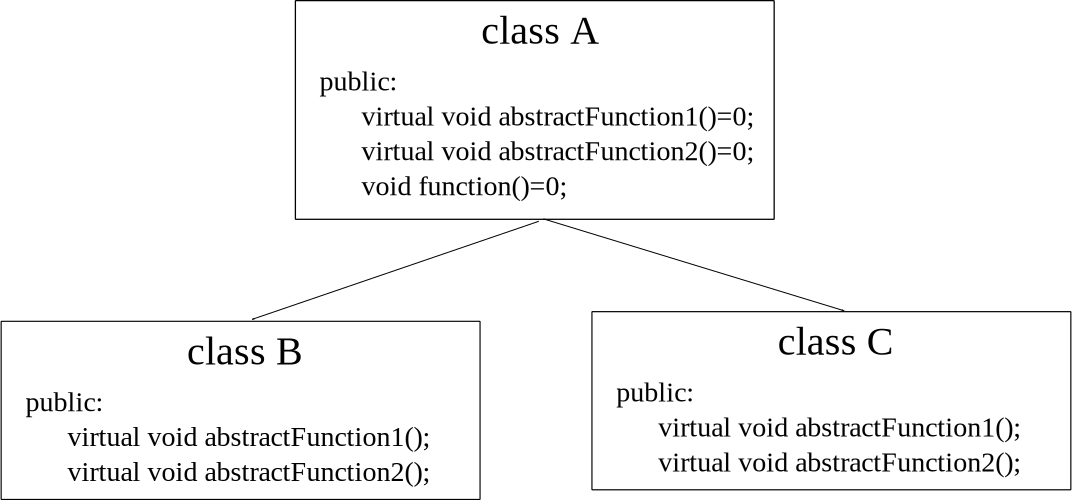
\includegraphics[width=0.5\textwidth]{imgs/UserManual/abstract.pdf}
\caption{Abstract class. Used through the whole program}
\label{fig:abstract}
\end{figure}

In order to illustrate how this technique is used here see Figure \ref{fig:abstract}. The class A contains two pure virtual functions (that makes the class A abstract). The class A does not implement any of its virtual functions. Instead, all virtual functions must be implemented by the subclasses B and C. For example, let's imagine that the class A corresponds to a classElements (where we do not care about the type of elements). Then the subclass B becomes classTriangles, in which the virtual functions are implemented, for example, the function to get the nodes that build the element (which depends on the type of elements). For the subclass C, that can be classTetrahedra, the implementation of the virtual functions are different, for example, the function to get the nodes, but the declaration of the functions is common for both subclasses. This so-called virtual inheritance is exploited through the whole program. We can plug another subclass D, that can be other type of element, as long as ALL virtual functions of the abstract class are implemented. The documentation generated by Doxygen (make documentation) can be very useful to follow the class trees.


\begin{figure}[htb]
\centering
\includegraphics[width=0.7\textwidth]{imgs/UserManual/structure_MuPhiSim.png}
\caption{General structure of MuPhiSim}
\label{fig:generalStruct}
\end{figure}

\begin{figure}[htb]
    \centering
    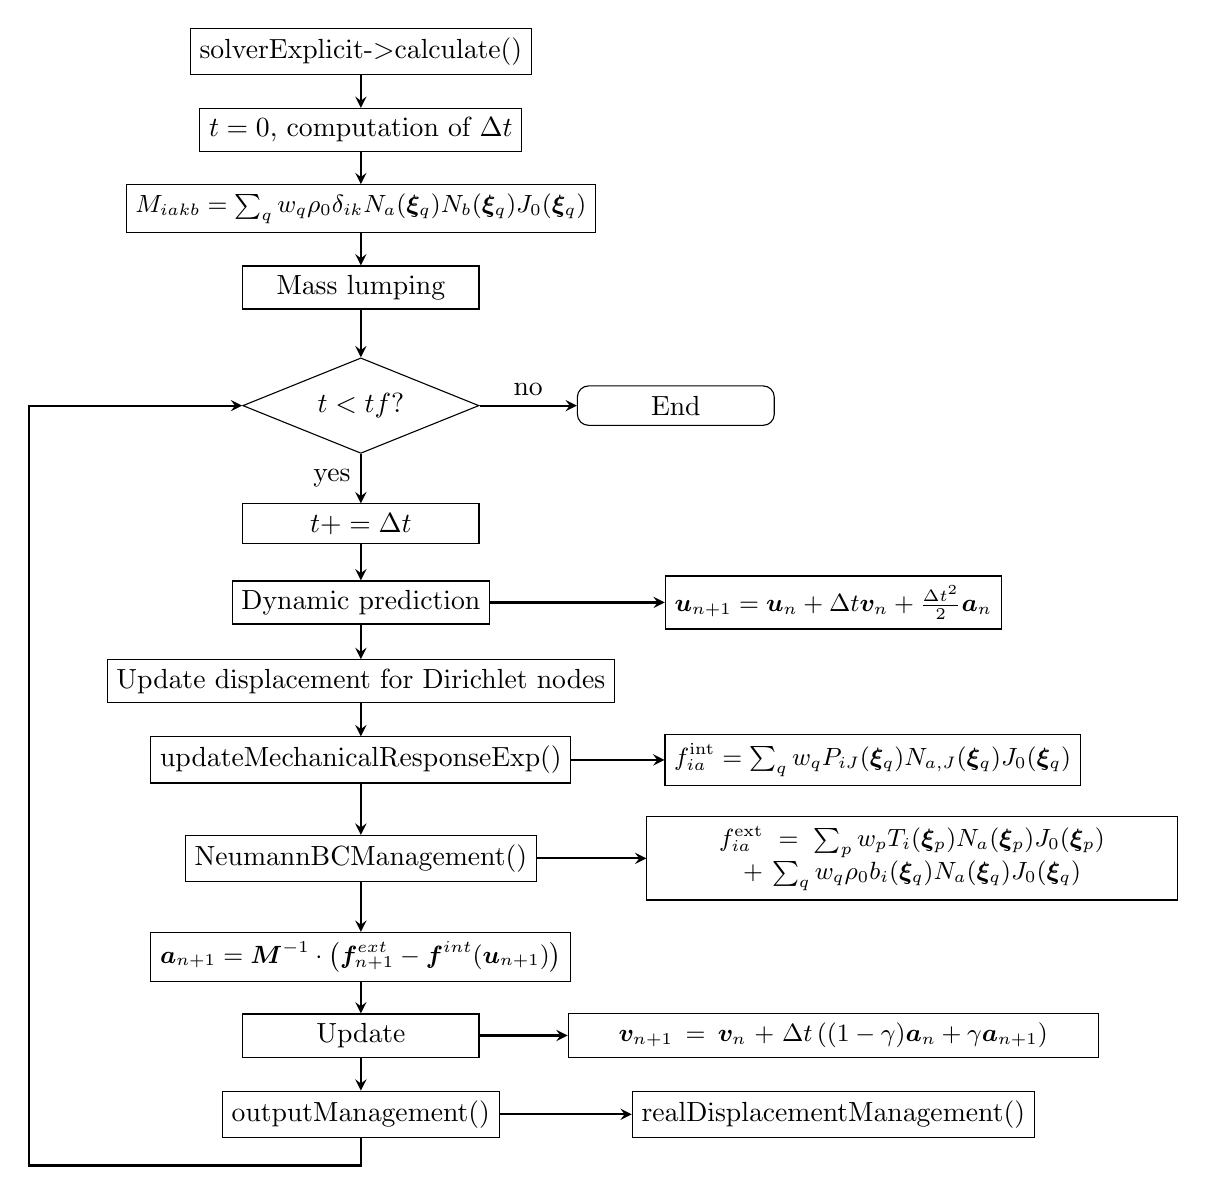
\begin{tikzpicture}[node distance=2cm]
        \node (start) [block] {solverExplicit-$>$calculate()};
        \node (blo1) [block, below of=start, yshift=+1cm] {$t=0$, computation of $\Delta t$};
        \node (blo2) [block, below of=blo1, yshift=+1cm] {\small $M_{iakb} = \sum_q w_q \rho_0 \delta_{ik} N_{a}(\bm{\xi}_q) N_{b}(\bm{\xi}_q) J_0(\bm{\xi}_q)$};
        \node (blo3) [block, below of=blo2, yshift=+1cm] {Mass lumping};
        \node (dec1) [choix, below of=blo3, aspect=2, yshift=+0.5cm] {$t<tf$?};
        \node (blo32) [block, below of=dec1, yshift=+0.5cm] {$t += \Delta t$};
        \node (stop1) [terminus, right of=dec1, xshift=+2cm] {End};
        \node (blo41) [block, below of=blo32, yshift=+1cm] {Dynamic prediction};
        \node (blo42) [block, right of=blo41, xshift=+4cm] {    \small $\bm{u}_{n+1} = \bm{u}_{n} + \Delta t {\bm{v}}_{n} + \frac{\Delta t^2}{2} {\bm{a}}_{n}$ };
        \node (blo43) [block, below of=blo41, yshift=+1cm] {Update displacement for Dirichlet nodes};
        \node (blo5) [block, below of=blo43, yshift=+1cm] {updateMechanicalResponseExp()};
        \node (blo6) [block, right of=blo5, xshift=+4.5cm] {\small $f_{ia}^{\text{int}} = \sum_q w_q  P_{iJ}(\bm{\xi}_q) N_{a,J}(\bm{\xi}_q) J_0(\bm{\xi}_q)$};
        \node (blo7) [block, below of=blo5, yshift=+0.75cm] {NeumannBCManagement()};
        \node (blo72) [block2, right of=blo7, xshift=+5cm] {\small $f_{ia}^{\text{ext}} = \sum_p w_p T_{i}(\bm{\xi}_p) N_{a}(\bm{\xi}_p)  J_0(\bm{\xi}_p)$ + $\sum_q w_q \rho_0 b_{i}(\bm{\xi}_q) N_{a}(\bm{\xi}_q)  J_0(\bm{\xi}_q)$};
        \node (blo8) [block, below of=blo7, yshift=+0.75cm] {\small ${\bm{a}}_{n+1} = \bm{M}^{-1}\cdot \left(\bm{f}^{ext}_{n+1} - \bm{f}^{int}(\bm{u}_{n+1})\right)$};
        \node (blo9) [block, below of=blo8, yshift=+1cm] {Update};
        \node (blo10) [block2, right of=blo9, xshift=+4cm] {\small $\bm{v}_{n+1} = \bm{v}_{n} + \Delta t \left( (1-\gamma)\bm{a}_n + \gamma \bm{a}_{n+1}\right) $};
        \node (blo11) [block, below of=blo9, yshift=+1cm] {outputManagement()};
        \node (blo12) [block, right of=blo11, xshift=+4cm] {realDisplacementManagement()};

        \draw [arrow] (start) -- (blo1);
        \draw [arrow] (blo1) -- (blo2);
        \draw [arrow] (blo2) -- (blo3);
        \draw [arrow] (blo3) -- (dec1);
        \draw [arrow] (dec1) -- node[anchor=south] {no} (stop1);
        \draw [arrow] (dec1) -- node[anchor=east] {yes} (blo32);
        \draw [arrow] (blo32) -- (blo41);
        \draw [arrow] (blo41) -- (blo42);
        \draw [arrow] (blo41) -- (blo43);
        \draw [arrow] (blo43) -- (blo5);
        \draw [arrow] (blo5) -- (blo7);
        \draw [arrow] (blo5) -- (blo6);
        \draw [arrow] (blo7) -- (blo72);
        \draw [arrow] (blo7) -- (blo8);
        \draw [arrow] (blo8) -- (blo9);
        \draw [arrow] (blo9) -- (blo10);
        \draw [arrow] (blo9) -- (blo11);
        \draw [arrow] (blo11) -- (blo12);
        \draw [arrow] (blo11.south) |- ++(-120pt,-10pt) |- (dec1.west);
    \end{tikzpicture}
    \caption{Structure of MuPhiSim Explicit Solver}
    \label{fig:solverExp}
\end{figure}

\begin{figure}[htb]
    \centering
    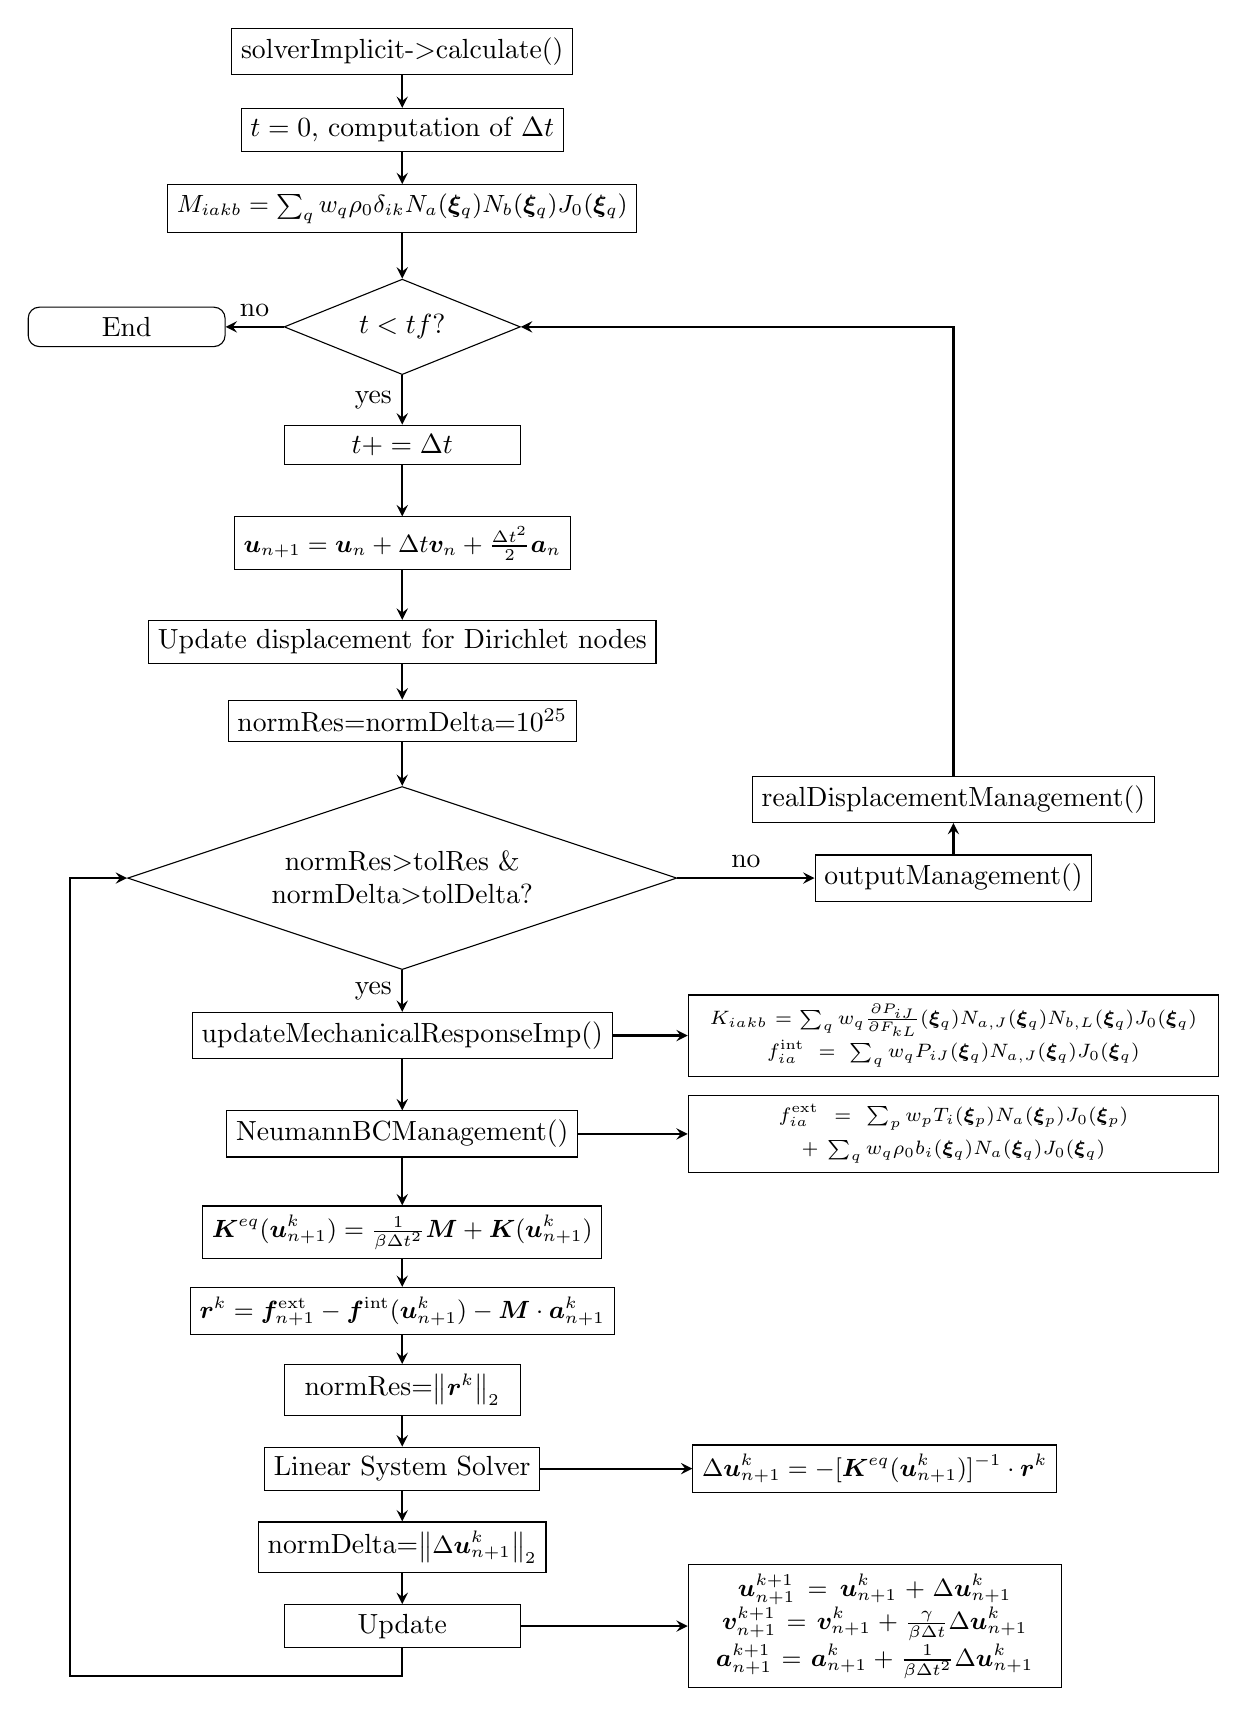
\begin{tikzpicture}[node distance=2cm]
        \node (start) [block] {solverImplicit-$>$calculate()};
        \node (blo1) [block, below of=start, yshift=+1cm] {$t=0$, computation of $\Delta t$};
        \node (blo2) [block, below of=blo1, yshift=+1cm] {\small $M_{iakb} = \sum_q w_q \rho_0 \delta_{ik} N_{a}(\bm{\xi}_q) N_{b}(\bm{\xi}_q) J_0(\bm{\xi}_q)$};
        \node (dec1) [choix, below of=blo2, aspect=2, yshift=+0.5cm] {$t<tf$?};
        \node (blo3) [block, below of=dec1, yshift=+0.5cm] {$t += \Delta t$};
        \node (stop1) [terminus, left of=dec1, xshift=-1.5cm] {End};
        \node (blo4) [block, below of=blo3, yshift=+0.75cm] {\small $\bm{u}_{n+1} = \bm{u}_{n} + \Delta t {\bm{v}}_{n} + \frac{\Delta t^2}{2} {\bm{a}}_{n}$};
        \node (blo6) [block, below of=blo4, yshift=+0.75cm] {Update displacement for Dirichlet nodes};
        \node (blo7) [block, below of=blo6, yshift=+1cm] {normRes=normDelta=$10^{25}$};
        \node (dec2) [choix2, below of=blo7, aspect=3, yshift=-0cm] {normRes$>$tolRes \& normDelta$>$tolDelta?};
        \node (blo8) [block, right of=dec2, xshift=+5cm] {outputManagement()};
        \node (blo9) [block, above of=blo8, yshift=-1cm] {realDisplacementManagement()};
        \node (blo10) [block, below of=dec2] {updateMechanicalResponseImp()};
        \node (blo11) [block2, right of=blo10, xshift=+5cm] {\scriptsize $K_{iakb} = \sum_q w_q  \frac{\partial P_{iJ}}{\partial F_{kL}}(\bm{\xi}_q) N_{a,J}(\bm{\xi}_q) N_{b,L}(\bm{\xi}_q) J_0(\bm{\xi}_q)$ $f_{ia}^{\text{int}} = \sum_q w_q  P_{iJ}(\bm{\xi}_q) N_{a,J}(\bm{\xi}_q) J_0(\bm{\xi}_q)$};
        \node (blo12) [block, below of=blo10, yshift=+0.75cm] {NeumannBCManagement()};
        \node (blo13) [block2, right of=blo12, xshift=+5cm] {\scriptsize $f_{ia}^{\text{ext}} = \sum_p w_p T_{i}(\bm{\xi}_p) N_{a}(\bm{\xi}_p)  J_0(\bm{\xi}_p)$ + $\sum_q w_q \rho_0 b_{i}(\bm{\xi}_q) N_{a}(\bm{\xi}_q)  J_0(\bm{\xi}_q)$};
        \node (blo14) [block, below of=blo12, yshift=+0.75cm] {\small $\bm{K}^{eq}(\bm{u}^{k}_{n+1}) = \frac{1}{\beta \Delta t^2} \bm{M} + \bm{K} (\bm{u}^{k}_{n+1})$ };
        \node (blo15) [block, below of=blo14, yshift=+1cm] {\small $\bm{r}^k = \bm{f}^{\text{ext}}_{n+1} - \bm{f}^{\text{int}}(\bm{u}^k_{n+1}) - \bm{M}\cdot \bm{a}^k_{n+1}$};
        \node (blo16) [block, below of=blo15, yshift=+1cm] {normRes=\small $\left\lVert \bm{r}^k\right\rVert_2$};
        \node (blo17) [block, below of=blo16, yshift=+1cm] {Linear System Solver};
        \node (blo18) [block, right of=blo17, xshift=+4cm] {\small $ \Delta \bm{u}^k_{n+1} = - [\bm{K}^{eq}(\bm{u}^{k}_{n+1})]^{-1} \cdot \bm{r}^{k}$};
        \node (blo19) [block, below of=blo17, yshift=+1cm] {normDelta=\small $\left\lVert \Delta \bm{u}^k_{n+1}\right\rVert_2$};
        \node (blo20) [block, below of=blo19, yshift=+1cm] {Update};
        \node (blo21) [block3, right of=blo20, xshift=+4cm] {\small ${\bm{u}}^{k+1}_{n+1} = {\bm{u}}^{k}_{n+1} + \Delta \bm{u}^k_{n+1}$
        ${\bm{v}}^{k+1}_{n+1} = {\bm{v}}^{k}_{n+1} + \frac{\gamma}{\beta \Delta t} \Delta \bm{u}^k_{n+1}$
        ${\bm{a}}^{k+1}_{n+1} = {\bm{a}}^{k}_{n+1} + \frac{1}{\beta \Delta t^2} \Delta \bm{u}^k_{n+1}$};


        \draw [arrow] (start) -- (blo1);
        \draw [arrow] (blo1) -- (blo2);
        \draw [arrow] (blo2) -- (dec1);
        \draw [arrow] (dec1) -- node[anchor=south] {no} (stop1);
        \draw [arrow] (dec1) -- node[anchor=east] {yes} (blo3);
        \draw [arrow] (blo3) -- (blo4);
        \draw [arrow] (blo4) -- (blo6);
        \draw [arrow] (blo6) -- (blo7);
        \draw [arrow] (blo7) -- (dec2);
        \draw [arrow] (dec2) -- node[anchor=south] {no} (blo8);
        \draw [arrow] (dec2) -- node[anchor=east] {yes} (blo10);
        \draw [arrow] (blo8) -- (blo9);
        \draw [arrow] (blo9.north) |- (dec1.east);
        \draw [arrow] (blo10) -- (blo11);
        \draw [arrow] (blo10) -- (blo12);
        \draw [arrow] (blo12) -- (blo13);
        \draw [arrow] (blo12) -- (blo14);
        \draw [arrow] (blo14) -- (blo15);
        \draw [arrow] (blo15) -- (blo16);
        \draw [arrow] (blo16) -- (blo17);
        \draw [arrow] (blo17) -- (blo18);
        \draw [arrow] (blo17) -- (blo19);
        \draw [arrow] (blo19) -- (blo20);
        \draw [arrow] (blo20) -- (blo21);
        \draw [arrow] (blo20.south) |- ++(-120pt,-10pt) |- (dec2.west);
 \end{tikzpicture}
    \caption{Structure of MuPhiSim Implicit Dynamic Solver}
    \label{fig:solverID}
\end{figure}

\begin{figure}[h!]
    \centering
    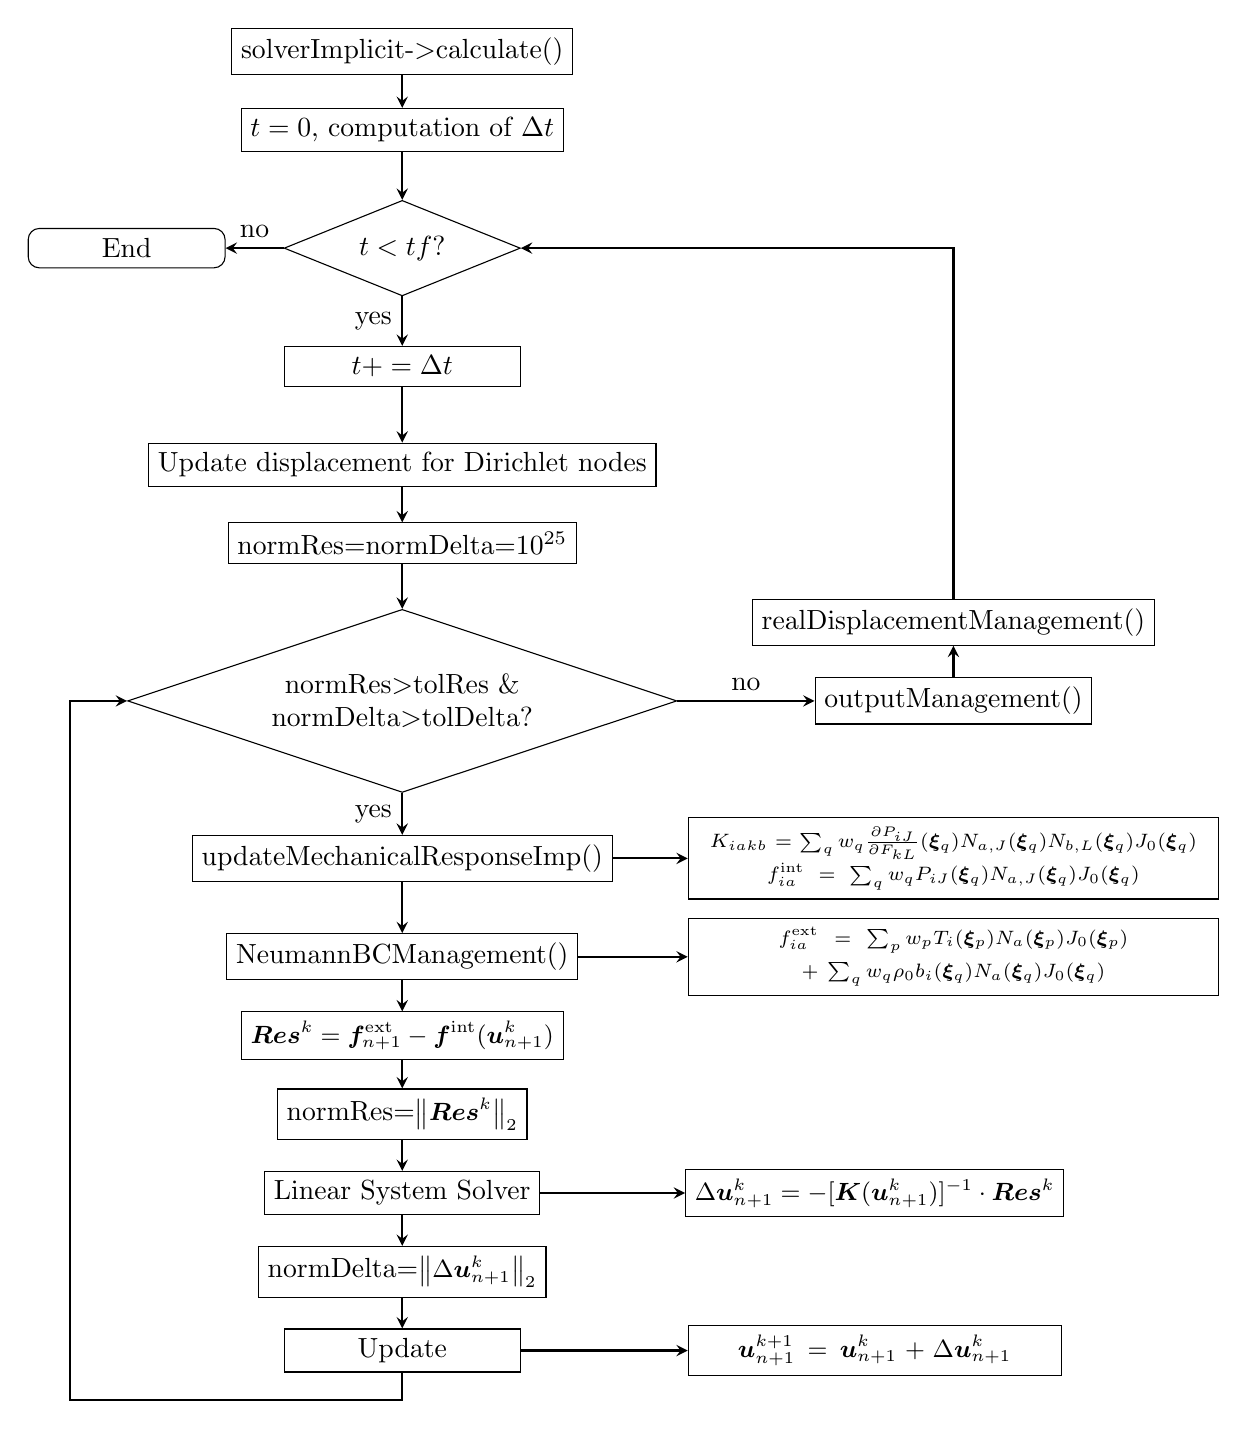
\begin{tikzpicture}[node distance=2cm]
        \node (start) [block] {solverImplicit-$>$calculate()};
        \node (blo1) [block, below of=start, yshift=+1cm] {$t=0$, computation of $\Delta t$};
        \node (dec1) [choix, below of=blo1, aspect=2, yshift=+0.5cm] {$t<tf$?};
        \node (blo3) [block, below of=dec1, yshift=+0.5cm] {$t += \Delta t$};
        \node (stop1) [terminus, left of=dec1, xshift=-1.5cm] {End};
        \node (blo6) [block, below of=blo3, yshift=+0.75cm] {Update displacement for Dirichlet nodes};
        \node (blo7) [block, below of=blo6, yshift=+1cm] {normRes=normDelta=$10^{25}$};
        \node (dec2) [choix2, below of=blo7, aspect=3, yshift=-0cm] {normRes$>$tolRes \& normDelta$>$tolDelta?};
        \node (blo8) [block, right of=dec2, xshift=+5cm] {outputManagement()};
        \node (blo9) [block, above of=blo8, yshift=-1cm] {realDisplacementManagement()};
        \node (blo10) [block, below of=dec2] {updateMechanicalResponseImp()};
        \node (blo11) [block2, right of=blo10, xshift=+5cm] {\scriptsize $K_{iakb} = \sum_q w_q  \frac{\partial P_{iJ}}{\partial F_{kL}}(\bm{\xi}_q) N_{a,J}(\bm{\xi}_q) N_{b,L}(\bm{\xi}_q) J_0(\bm{\xi}_q)$ $f_{ia}^{\text{int}} = \sum_q w_q  P_{iJ}(\bm{\xi}_q) N_{a,J}(\bm{\xi}_q) J_0(\bm{\xi}_q)$};
        \node (blo12) [block, below of=blo10, yshift=+0.75cm] {NeumannBCManagement()};
        \node (blo13) [block2, right of=blo12, xshift=+5cm] {\scriptsize $f_{ia}^{\text{ext}} = \sum_p w_p T_{i}(\bm{\xi}_p) N_{a}(\bm{\xi}_p)  J_0(\bm{\xi}_p)$ + $\sum_q w_q \rho_0 b_{i}(\bm{\xi}_q) N_{a}(\bm{\xi}_q)  J_0(\bm{\xi}_q)$};
        \node (blo15) [block, below of=blo12, yshift=+1cm] {\small $\bm{Res}^k = \bm{f}^{\text{ext}}_{n+1} - \bm{f}^{\text{int}}(\bm{u}^k_{n+1})$};
        \node (blo16) [block, below of=blo15, yshift=+1cm] {normRes=\small $\left\lVert \bm{Res}^k\right\rVert_2$};
        \node (blo17) [block, below of=blo16, yshift=+1cm] {Linear System Solver};
        \node (blo18) [block, right of=blo17, xshift=+4cm] {\small $ \Delta \bm{u}^k_{n+1} = - [\bm{K}(\bm{u}^{k}_{n+1})]^{-1} \cdot \bm{Res}^{k}$};
        \node (blo19) [block, below of=blo17, yshift=+1cm] {normDelta=\small $\left\lVert \Delta \bm{u}^k_{n+1}\right\rVert_2$};
        \node (blo20) [block, below of=blo19, yshift=+1cm] {Update};
        \node (blo21) [block3, right of=blo20, xshift=+4cm] {\small ${\bm{u}}^{k+1}_{n+1} = {\bm{u}}^{k}_{n+1} + \Delta \bm{u}^k_{n+1}$};


        \draw [arrow] (start) -- (blo1);
        \draw [arrow] (blo1) -- (dec1);
        \draw [arrow] (dec1) -- node[anchor=south] {no} (stop1);
        \draw [arrow] (dec1) -- node[anchor=east] {yes} (blo3);
        \draw [arrow] (blo3) -- (blo6);
        \draw [arrow] (blo6) -- (blo7);
        \draw [arrow] (blo7) -- (dec2);
        \draw [arrow] (dec2) -- node[anchor=south] {no} (blo8);
        \draw [arrow] (dec2) -- node[anchor=east] {yes} (blo10);
        \draw [arrow] (blo8) -- (blo9);
        \draw [arrow] (blo9.north) |- (dec1.east);
        \draw [arrow] (blo10) -- (blo11);
        \draw [arrow] (blo10) -- (blo12);
        \draw [arrow] (blo12) -- (blo13);
        \draw [arrow] (blo12) -- (blo15);
        \draw [arrow] (blo15) -- (blo16);
        \draw [arrow] (blo16) -- (blo17);
        \draw [arrow] (blo17) -- (blo18);
        \draw [arrow] (blo17) -- (blo19);
        \draw [arrow] (blo19) -- (blo20);
        \draw [arrow] (blo20) -- (blo21);
        \draw [arrow] (blo20.south) |- ++(-120pt,-10pt) |- (dec2.west);
     \end{tikzpicture}
    \caption{Structure of MuPhiSim Implicit Static Solver}
    \label{fig:solverIS}
\end{figure}



%%%%%%%%%%%%%%%%%%%%%%%%%%%%%%%%%%%%%%%% CHAPTER 2 %%%%%%%%%%%%%%%%%%%%%%%%%%%%%%%%%%%%%%%%%%%%

\chapter{INPUT FILES}\label{Chapter:inputs}
\section{Introduction}
\textit{MuPhiSim} follows the Abaqus .inp format with some differences that are clearly specified in the following sections. The input file must be inside the input folder and should be named with the .inp extension e.g., \texttt{example.inp}. The program is case sensitive and every single space or comma can make a difference. Follow the next sections thoroughly in order to avoid problems. As a general rule, it does not matter in what order the keywords appear in the input file. However, several keywords must be grouped (they will be highlighted in the following sections). All keywords will be preceded by a star symbol \textbf{*}. Although \textit{MuPhiSim} is programmed in C++ and thus follows zero notation in the arrays, that is fully independent of the input file, and the numbers that appear therein. Therefore, the enumerations within the input file must start from 1. All columns are separated by commas in the input file. There is also an option to generate a \textit{MuPhiSim} input file using a GUI tool, although the users are strongly advised to read through the manual input section and familiarize themselves with the specifics of \textit{MuPhiSim} input.

\section{Python code: python-gmsh}
The input file can be easily created using \emph{python-gmsh} python project located in \emph{tools/python-gmsh}. The mesh is created using Gmsh (\hyperlink{http://gmsh.info/}{http://gmsh.info/}). 

Please refer to \emph{tools/python-gmsh/ReadMe.md} for more information.


\section{GUI}
\subsection{Description}
This tool reads Abaqus input files, takes input from the user and produces a corresponding \textit{MuPhiSim} file. To define a certain domain in \textit{MuPhiSim}, the input file has to contain a fully written out list of nodes/elements. This tool was initially meant to simply read all such sets from Abaqus and print them out, but has since grown into an application that allows the users to create full \textit{MuPhiSim} input files with aid of a graphical user interface. It should be noted that the tool does not necessarily encapsulate all features of \textit{MuPhiSim}, and does not automatically include all updates done to the main code, such as for example addition of new constitutive models. Use this tool with a pinch of salt, and refer to the manual input section if in doubt.
\subsection {Note to developers}
The tool consists of two Python scripts, MuPhiSiminput.py and parser.py. Parser.py handles the logic, while MuPhiSiminput.py builds the GUI and reads the user input. Most minor changes, for instance addition of a material model, will be done in the MuPhiSiminput.py script, in this case, a simple modification of the material box class. However, the developer should look at the relevant section of the parser script, in case the modification to the input is incompatible with its processing.
\subsection{Installation}
The parser tool can be found in tools/GUI folder, and requires Python 3.0 or higher to run. It also requires the Tkinter module, which can be installed by running the following console line:\\
\$sudo apt-get install python3-tk\\
To launch the GUI app, run:\\
\$python3 MuPhiSiminput.py\\

\begin{figure}[h!]
    \centering
    \includegraphics[width=1\textwidth]{imgs/UserManual/GUI.png}
    \caption{GUI window}
    \label{fig:GUIWindow}
\end{figure}

\subsection{Usage}
\begin{enumerate}
\item\textbf{File I/O} - After running the script, a window will appear prompting the user to open an Abaqus file. Select the relevant file, as the app will get all the nodes, elements and sets. Afterwards, the main GUI window with an \textit{MuPhiSim} logo should appear, such as shown in Figure \ref{fig:GUIWindow}. Choose where the output should be written by using the "Save as" button, and if no file with the specified name exists, such file will be created.

\item\textbf{Region Set} - Define the FEM and/or MM regions using the drop-down menu, which will contain all sets created in Abaqus. One may select both MM and FEM sets, or if all nodes/elements are to be used, simply select "All". The user can also create custom computation partitions for the mesh. To do so, select the number of processors that will be used, and assign node and element sets to each processor. Also surface order allows the user to control the integration order for surface elements. Keep in mind that surface order must be less than or equal to overall bulk order.

\item\textbf{Solver Options} - Type in the desired number of solvers, and click "Confirm". Fill in all the boxes using appropriate format, if unclear, refer to the manual input section. The time is specified for each solver, and the parser will produce the correct ranges in the \textit{MuPhiSim} file, in the case of Figure \ref{fig:GUIWindow}, [0,1] for the first solver and [1,3] for the second. The BC displacement sets should be input manually, as there can be several. These sets should be separated by commas, keeping in mind these are sets of nodes, make sure the name is exactly as it appears in the Abaqus file. One can get a complete list of all sets by simply scrolling through one of the selection boxes for sets. "BC DOFs" refers to the constraints that should be applied to the named BC sets. These should be input as ordered tuples separated by commas. If one wishes to constrain only some of the DOFs in that set, the other DOFs should be substituted by a question mark (?). The number of DOFs is determined by the nature of the simulation, so for a 3D simulation with an extra DOF, the user can input up to 4 DOFs per tuple. For Figure \ref{fig:GUIWindow}, the first solver will have only constrained all first DOFs in Set1 to 0, and all second DOFs of all nodes in Set2 to 1 unit. The second solver fixes first, second and third DOF in Set1 to 0. Forces output allows the user to print the equivalent forces for Dirichlet nodes. The user specifies the frequency of the output (frequency of 2 means that forces will be written twice per unit time), the set of Dirichlet nodes as well as the DOF of interest. Question mark again omits the DOF, while any number will enable that particular DOF. So in order to write only z-direction, the input can be (?,?,1). The forces are defined inside the solver environment, and each solver will produce a .csv file in the output folder.

* In order to avoid duplicating BC on the shared nodes, for the cases with FEM and MM elements / nodes, the first set to be entered must be the one in which we are going to define the desired BC for the shared nodes.

\item\textbf{Material Laws} - Select number of materials to be present in the simulation, and press "Confirm". Fill in the boxes, keeping in mind that every element present in the simulation should have exactly one material assigned to it. However, extra DOFs are defined in the material section, so that does not apply to previous statement. After choosing a material model, fill in all parameters, separating them with commas if needed.

\item\textbf{Boundary Conditions} - Select the number of Neumann boundary conditions desired, keeping in mind these are not dependent on the number of solvers, as they are defined outside the solver environment and rather depend on time. Pressures are applied to surfaces of elements, and these surfaces should be entered into the "Surface" box. If the elements to which pressure should be applied is defined in Abaqus using "Pressure" loading condition, then once the file is loaded into the GUI, the surface to which pressure is applied should appear next to the name of the set. In the example used, the set was named "pre", but appears as "\_pre\_S2", which means that the surface of interest is 2. Nodal force is quite trivial to use, simply select the set of nodes, time interval, and define a force vector. Moreover, it permits to define the different Neumann BC for extradof. Current Inst, define the Neumann BC for electrophysiology. The user has to select the set of elements, time interval, and define a amount of current. Moreover, heat inst, define a surface heat flux for heat equation. As well as pressure, surface heat flux is applied on a surface. The user has to select the surface to which heat flux is applied (this should appear next to the name of the set) , time interval, heat flux vector (the last term of the vector will be zero for 2D) and the surface of interest (see Figure \ref{fig:GUIWindow-EXTRADOF}).

\end{enumerate}
When the input is complete, click "Execute", and the \textit{MuPhiSim} file should be written to the location specified by the user.
\begin{figure}[h!]
    \centering
    \includegraphics[width=0.8\textwidth]{imgs/UserManual/GUI-EXTRADOF.png}
    \caption{GUI window-extradof boundary conditions}
    \label{fig:GUIWindow-EXTRADOF}
\end{figure}

\section{Manual input}
\subsection{Nodes}
The list of nodes should begin with the keyword \textbf{*Node} followed by the list of nodes enumerated in the first column and then each coordinate 2D/3D in the following columns (exactly the same format as Abaqus).

Example:
\begin{lstlisting}
 *Node
 1, 0.4, 0.9, 4
 ...
\end{lstlisting}


\subsection{Elements}
The list of elements should begin with the keyword \textbf{*Element, type=typeOfElement} followed by the list of elements enumerated in the first column and then each node that builds the element should be specified in 2D/3D (exactly the same format as Abaqus). The names of the elements follow the Abaqus nomenclature. The elements available so far in \textit{MuPhiSim} are the following:
\begin{enumerate}
\item Linear segments \textbf{typeOfElement=Segments} (1D) It is used for the boundaries (not to carry out simulations in 1D)
\item Linear triangles \textbf{typeOfElement=CPS3} (2D)
\item Linear squares \textbf{typeOfElement=CPE4} (2D)
\item Linear tetrahedra \textbf{typeOfElement=C3D4} (3D)
\item Linear hexahedra \textbf{typeOfElement=C3D8} (3D)
\item Quadratic triangles \textbf{typeOfElement=CPS6} (2D)
\item Quadratic tetrahedra \textbf{typeOfElement=C3D10} (3D)
\item Quadratic triangles with linear surfaces \textbf{typeOfElement=CPS6\_lin\_surf} (2D)
\item Quadratic tetrahedra with linear surfaces \textbf{typeOfElement=C3D10\_lin\_surf} (3D)
\end{enumerate}

Example:
\begin{lstlisting}
 *Element, type=C3D4
 1, 227, 137, 219
 ...
\end{lstlisting}

\subsubsection*{Implementation of new type of elements}
Following the concepts shown in Section \ref{sec:concept}, the inheritance diagram for the classElements is shown in Figure \ref{fig:classElements}. All new elements will be new classes that inherit from classElements. It is recommended to copy/paste an existing type of element and modify it accordingly. See the Doxygen documentation to have the list of virtual functions and what they do. This is easy to do by navigating the html files generated by Doxygen.

\begin{figure}[htb]
    \centering
    \includegraphics[width=1\textwidth]{imgs/UserManual/classElements.pdf}
    \caption{Class elements inheritance diagram}
    \label{fig:classElements}
\end{figure}

When a new type of element is added, the input file should be also modified accordingly. It is recommended to copy/paste the same structure of the input file of the existing type of elements.

\subsection{Distribution in FEM and/or MM}
The list of nodes and elements of each type should be provided (in the future, some algorithms will be implemented to define such distribution). The keywords are \textbf{*FEM/*MM Nodes} and \textbf{*FEM/*MM Elements} followed by the list (one label per line) of nodes/elements by means of the corresponding label of the full list of nodes/elements. If all nodes/elements in the simulation are FEM/MM the keyword \textbf{All} can be used instead of repeating the whole list. This part is new compared to the traditional input files for Abaqus.

\subsection{Computation region assignment in parallel}
In parallel mode, \textit{MuPhiSim} automatically partitions the mesh and assigns the regions to the processors. However, there is an option for the user to assign what region the different processors will be responsible for. To do so, the user first assigns all the nodes to the processors, and then all the corresponding elements. The syntax for defining a region for i-th CPU is as following:

\begin{lstlisting}
*NSET="Name of the region"
*CPU=i
\end{lstlisting}

where $i \in [1, n]$ and $n$ is the total number of CPUs in the simulation. "Name of the region" should be replaced by a user-defined name, and all the subsequent lines should list the nodes in that region. Similarly, the elements that the i-th CPU is responsible for should be written using the following syntax:

\begin{lstlisting}
*ELSET="Name of the region"
*CPU=i
\end{lstlisting}

and the following lines should list all elements in that region. Below is a sample input for 2 processors:

\begin{lstlisting}
*NSET=region1
*CPU=1
1
2
5
6
*NSET=region2
*CPU=2
2
3
4
5
*ELSET=region1
*CPU=1
1
2
*ELSET=region2
*CPU=2
3
4
\end{lstlisting}

The user should keep in mind that in case of manual partitioning, the input file must contain the same number of CPUs as specified when running MuPhiSim in the command line.


\subsection{Solver}
The choice of the solver should be defined by the keyword \textbf{*SOLVER, TYPE}, where  \textbf{TYPE} can be either \textbf{EXPLICIT}, \textbf{IMPLICIT} (dynamic) or \textbf{IMPLICIT STATIC}. The keyword \textbf{*END SOLVER} should be at the end of the solver definition. The number of solvers is not limited, and the solvers must be distributed continuously along the time of simulation. \\

If implicit and explicit (dynamic) solvers are used, the keyword \textbf{*FSI} can be used to run a coupled simulation with OpenFOAM. It must be followed by the list of nodes at the coupling interface by means of the corresponding label in the full list of nodes. See chapter 13 for more details.\\

A C++ file - input\_file\_generation.cpp - writes the input file for the simple example implemented in the \textbf{quickstart} folder. It generates the input file directly at the right place, i.e. the
input folder of \textit{MuPhiSim}.\\

The keyword \textbf{*Scale Factor} can be used to define the scale factor to be applied to the critical time step. Actually, \textbf{dt = $<$Scale factor$>$ * $<$Critical timestep$>$}. The value should be in the next line after the keyword.\\

The keyword \textbf{*Number Of Steps} can be used to define the number of time steps in the implicit and implicit static solvers. Once \textbf{*Number Of Steps} is given, \textbf{*Scale Factor} is not used.\\

The keyword \textbf{*TIME STEPPING PLAN} can be used to define the time stepping plan in static solver. For example, a simulation from 0 to 1s following the plan: 0s-0.1s with 10 steps, 0.1s-0.5s with 3 steps, and 0.5s-1s with 50 steps can be performed with the following plan
\begin{lstlisting}
*TIME STEPPING PLAN
0.1, 10
0.5, 3
1, 50
\end{lstlisting}

It is noted that \textbf{*Scale Factor} must be used in an explicit scheme to define the time step. In the implicit and implicit static schemes, the time step is defined first by the first line in \textbf{*TIME STEPPING PLAN}. If it is not available, \textbf{*Number Of Steps} is used. If the latter is still not available, \textbf{*Scale Factor}.

The maximum time step can be constrained with the keyword \textbf{*Max Time Step}. For example, we can limit the time step in the implicit and implicit static simulation by a value of 0.01 using
\begin{lstlisting}
*Max Time Step
0.01
\end{lstlisting}

The automatic adaptive time stepping can be considered by using the keyword \textbf{*ADAPTIVE TIME STEP}. The idea is to adapt the time step for next step based on the convergence of the current step by a general relation
\begin{eqnarray*}
\Delta t_{new} = \text{f}(\Delta t_{prev}, ...)
\end{eqnarray*}
In the current version, only the power law is implemented as
\begin{eqnarray*}
\Delta t_{new} = \Delta t_{prev} \left(\frac{N_{opt}}{N_{iter}^{prev}} \right)^n
\end{eqnarray*}
where $N_{iter}^{prev}$ is the number of iterations to converge the solution in the current step, $N_{opt}$ is its expected value, $n$ is a positive real number. Using this function, the time step increases if the number of iterations required to converge the solution is smaller than the expected value and vice-versa. In the input file, the following line is added to activate this option
\begin{lstlisting}
*ADAPTIVE TIME STEP
POWER,6,0.5
\end{lstlisting}
where $N_{opt}=6$ and $n=0.5$.

The keyword \textbf{*Absolute Tolerance} ($10^{-12}$ by default) can be used to define the absolute tolerance in the implicit and implicit static solvers.\\

The keyword \textbf{*Relative Tolerance} ($10^{-6}$ by default) can be used to define the relative tolerance in the implicit and implicit static solvers.\\

The keyword \textbf{*Max Iterations} (50 by default) can be used to define the maximal number of iteration in each time step in the implicit and implicit static solvers.\\

The keyword \textbf{*STIFFNESS MATRIX} is used to define the strategy of modifying the stiffness during an implicit (static) scheme. By default, the stiffness is updated every iteration at every time step. In some case, the modification of the stiffness can be planned as follows
\begin{itemize}
	\item The stiffness matrix is updated all time steps and iterations (this is also the default option in the solver)
	\begin{lstlisting}
	*STIFFNESS MATRIX, TYPE=CURRENT
	\end{lstlisting}
	\item One single stiffness matrix for all subsequent time steps and iterations
	\begin{lstlisting}
	*STIFFNESS MATRIX, TYPE=BEGINNING
	\end{lstlisting}
	\item The stiffness matrix is updated only at the beginning of each time step
	\begin{lstlisting}
	*STIFFNESS MATRIX, TYPE=INITIAL
	\end{lstlisting}
	\item The stiffness matrix is updated after kth iteration of each time step
	\begin{lstlisting}
	*STIFFNESS MATRIX, TYPE=ITERATION
	k
	\end{lstlisting}
	\item The stiffness matrix is updated after each n iteration of each time step
	\begin{lstlisting}
	*STIFFNESS MATRIX, TYPE=INTERVAL
	n
	\end{lstlisting}
\end{itemize}
It is noted that the \textbf{TYPE=BEGINNING} or \textbf{TYPE=INITIAL} should be used, as it reduces the computation cost (LU factorisation) since the matrix is factorised once but re-used through iterations without the need of re-factorising.

The stiffness matrix can be computed by perturbation without the need of the computation of tangents at the material law. This option can be activated by
\begin{lstlisting}
*TANGENT BY PERTURBATION
1e-8
\end{lstlisting}
where 1e-8 is a tolerance which can be introduced arbitrarily. This option is a very efficient way to obtain a good convergence rate.

If explicit solver is used, the keyword \textbf{*Bulk viscosity} or \textbf{*Dev viscosity} can be used to add an artificial bulk or deviatoric viscosity when first Piola-Kirchhoff tensor is computed. The default parameters for linear and quadratic coefficients are \{0.06,1.2\} for bulk viscosity and \{1,0.5\} for deviatoric viscosity. The user can change these values adding a second line.

Example :
\begin{lstlisting}
*Bulk viscosity
0.08,1.2
 ...
\end{lstlisting}

The keyword \textbf{*Outputs} can be used to define the number of output files if the number of time steps allows it. The value should be in the next line after the keyword.

In addition, there can be a second line after this keyword that relates to the internal variables. All the internal variables can be stored using \textbf{All, max} in that line, where \textbf{max} is the maximum number of internal variables. Some specific internal variables can be stored using their positions in the intVar array, e.g.,  \textbf{60, 2, 5} will store internal variables 2 and 5, while 60 is the maximum size of the internal variables. If the constitutive model does not have internal variables, zeros will be printed out in the output files. The default outputs are VMS, displacements and Cauchy Stress.

Example :

\begin{lstlisting}
 *Outputs
All, max
60, 2, 5
 ...
\end{lstlisting}

In a possible third line (without which, any internal variable will be given in the outputs), the first value is the maximum number of internal variables in the whole domain (regardless if there is more than one constitutive model). For example, if there is one constitutive model with 8 internal variables and another with 2, 8 must be provided to the program. It is the responsibility of the user to specify how the internal variables are stored in the intVars array. One 3x3 tensor corresponds to 9 spaces in the vector, etc. In each output file, the requested variables will be in a vector intVars, where each component corresponds to the specified position. After a comma, all the components which are desired in the output files must be provided in the intVars array. If position 6 is requested in the previous example, in the output, the elements with the constitutive model 1 (which had two variables) will have zeros assigned to these positions. If the constitutive models have some common internal variables that it would be useful to compare, make sure that they are placed in the same positions of the internal variable arrays, in order to be able to compare them in Paraview. Finally, if all internal variables are required, simply use All in the third line, and after a comma, provide the maximum number of internal variables in the domain.\\

The keyword \textbf{*Time} is used to define the time of the simulation for this particular solver. The initial and the final times should be in the next line, separated by comma.  \\

Dirichlet boundary conditions can be defined as a progressive ramp between $t_0$ and $t_f$ or instantaneously at $t_0$. For the latter, in implicit and explicit cases, the velocity is defined considering the time step instead of the total time. The keywords are \textbf{*BOUNDARY, TYPE=DISPLACEMENT RAMP} and \textbf{*BOUNDARY, TYPE=DISPLACEMENT INST}. The detection of instantaneous BC actives a boolean flag in inputFile.cpp \\
$\bm{----------------------------------}$\\
\} else if (line2.compare(0, 33, "*BOUNDARY, TYPE=DISPLACEMENT INST") == 0) \{ \\
flagInstantaneous = true; \\
$\bm{----------------------------------}$\\
this flag defines the construction of classDirichlet as
\\
$\bm{----------------------------------}$\\
if (flagInstantaneous) \{\\
                    \hspace*{0.5cm}//if flagInstantaneous = true Dirichlet BC are applied instantaneously\\
                    \hspace*{0.5cm}tempDirichlet = new classDirichlet(ndim, tempme, tempxyz, UU, direction, numNodes);\\
                \} else \{\\
                   \hspace*{0.5cm} //if flagInstantaneous = false Dirichlet BC they are applied as a ramp\\
                   \hspace*{0.5cm} tempDirichlet = new classDirichlet(ndim, tempme, tempxyz, UU, direction, numNodes,\\ \hspace*{0.5cm} duration);\\
                \}
 \\
$\bm{----------------------------------}$\\
Depending on the definition of Dirichlet BC, an integer, called \textit{flagDiri}, is be defined as 1 (ramp) or -1 (instantaneous) in classNodes, that will be used subsequently to apply the BC in each specific solver.\\
To specify the list of nodes with their corresponding displacements, each  node, direction [0-x, 1-y, 2-z], and the corresponding value of the displacement should be provided, e.g., $node$ $label, 1, 0.1$ which is read as a displacement in the y direction of 0.1 meters.

In a multiphics simulation, in which the keyword \textbf{*ExtraDof} is specified later in the material field, the boundary conditions of the extra-dofs can be also specified. For example, in an electro-mechanical or a thermal-mechanical problem, the electrical Dirichlet boundary condition $\Phi$ or temperature $\theta$ may be specified at the end of the line [0-x, 1-y, 2-z, 3-$\Phi$] in 3D or [0-x, 1-y, 2-$\Phi$] in 2D. If there are more than one extradof, e.g. electro-thermal-mechanical problem, the second extradof (and successive) Dirichlet boundary condition may be specified at the end of the line [0-x, 1-y, 2-z, 4-variable] in 3D or [0-x, 1-y, 3-variable] in 2D.\\

%Dirichlet boundary conditions are defined as a progressive ramp between t0 and tf. This fact has to be taken into account, specially in transient thermal analysis, since the final Dirichlet boundary conditions will not be reached until tf. This issue is solved defining two solver. In this regard, in the first solver we apply the Dirichlet boundary conditions for a short period of time, while the second solver maintain these BCs and lets the dynamic of the problem works.

%Example:
%\begin{lstlisting}
%*SOLVER, IMPLICIT STATIC
%*Scale Factor
%10000
%*Outputs
%200
%All, max
%*Time
%0, 1
%*BOUNDARY, TYPE=DISPLACEMENT
%1, 0, 0
%1, 2, 100
%2, 2, 100
%3, 2, 100
%4, 2, 100
%*END SOLVER
%**SOLVER, IMPLICIT STATIC
%*Scale Factor
%10000
%*Outputs
%200
%All, max
%*Time
%1, 1000
%*BOUNDARY, TYPE=DISPLACEMENT
%1, 0, 0
%1, 2, 0
%2, 2, 0
%3, 2, 0
%4, 2, 0
%*END SOLVER
%\end{lstlisting}

The keyword \textbf{*Forces} can be used to create another output file (format .csv) where the user can print the nodal forces among $x$, $y$ or $z$. On the first line, the user specifies the frequency of outputs (outputs per unit time). The user then specifies on the following lines the nodes that will be selected and for each node, the direction (0 for $x$, 1 for $y$ and 2 for $z$).

Example:
\begin{lstlisting}
...
*Forces
0.01
1, 0
2, 0
3, 0
4, 0
1, 1
2, 1
3, 1
4, 1
...\end{lstlisting}
Finally, the user can choose which
PETSc solver and preconditioner are employed to solve the system using the keywords \textbf{*PETSC\_SOLVER} and  \textbf{*PETSC\_PC}. The complete list of PETSc solvers and preconditioners can be found in the following links:\\
\url{https://www.mcs.anl.gov/petsc/petsc-current/docs/manualpages/KSP/KSPType.html#KSPType}\\
 \url{https://www.mcs.anl.gov/petsc/petsc-current/docs/manualpages/PC/PCType.html}\\

The following example shows the assignment of the iterative solver Conjugate Gradient (cg) with the Jacobi preconditioner (jacobi):
\begin{lstlisting}
...
*PETSC_SOLVER, cg
*PETSC_PC, jacobi
*END SOLVER
...\end{lstlisting}
Note that if the user does not introduce any PETSc solver and preconditioner through the keywords in the input file, the default iterative solver Conjugate Gradient (cg) is assigned with the default preconditioners LU and block Jacobi (bjacobi) for the sequential and parallel simulations, respectively. In general, the direct LU solver (by default in the code) is recommended for both sequential and parallel simulations.

\subsubsection*{Multisolvers}
To have two or more successive solvers, simply add their definition chronologically. The only requirement is that the time interval of each solver should be in agreement with each other without any gap.

Example:
\begin{lstlisting}
*SOLVER, EXPLICIT
*Scale Factor
0.01
*Outputs
100
All, 2
*Time
0, 820
*BOUNDARY, TYPE=DISPLACEMENT
   3, 0, 0
   4, 0, 0
   6, 0, 0
   7, 0, 0
  39, 0, 0
  101, 0, 0
  109, 1, 100
 110, 1, 100
 140, 1, 100
 347, 1, 100
 348, 1, 100
 349, 1, 100
   1, 0, 0
*END SOLVER
*SOLVER, EXPLICIT
*Scale Factor
0.01
*Outputs
100
All, 2
*Time
820, 10000
*BOUNDARY, TYPE=DISPLACEMENT
   3, 0, 0
 349, 1, 100
   1, 0, 0
*END SOLVER
\end{lstlisting}
\subsubsection*{Progressively activation/deactivation of elements} \textit{MuPhiSim} includes the option to activate/deactivate elements in every step. To use this option, see
\textit{Appendix A}.
\subsection{Neumann boundary conditions}

% I have to conclude this section with the explicit explanation of  Neumann and Dirichlet BCs from the implementation point of view. It is not straightforward.

%       // The displacements for the Dirichlet nodes should be the previous displacements. We are adding the Dirichlet influence in DirichletBCManagement, NOT HERE

%       // The dirichlet nodes are not taken into account in the criteria (The are forced!!!). We do not put ones. Instead, in order to homogenize the linear system, we keep K and multiply the right hand side by KK as well.

% // Correction; The correction for the Dirichlet nodes is not taken into account in the solution of the displacements. It is forced after the Newton loop

%     // Forcing the Dirichlet boundary condition after NR


% This is for the dynamic implicit

%   // // Julian: Mass does at the dirichlet nodes does not contribute with any inertia
%       // KKeq is overwritten in KK
%       // The dirichlet nodes are not taken into account in the criteria (The are forced!!!). We do not put ones. Instead, in order to homogenize the linear system, we keep K and multiply the right hand side by KK as well.

The Neumann BCs are defined globally. They should be defined out of the Solver environment, e.g just after the last solver. Force at the nodes will be imposed instantaneously whereas the pressure can be imposed either instantaneously or progressively as shown on fig. \ref{PressureInstRamp}.

\begin{figure}[h]
    \centering
    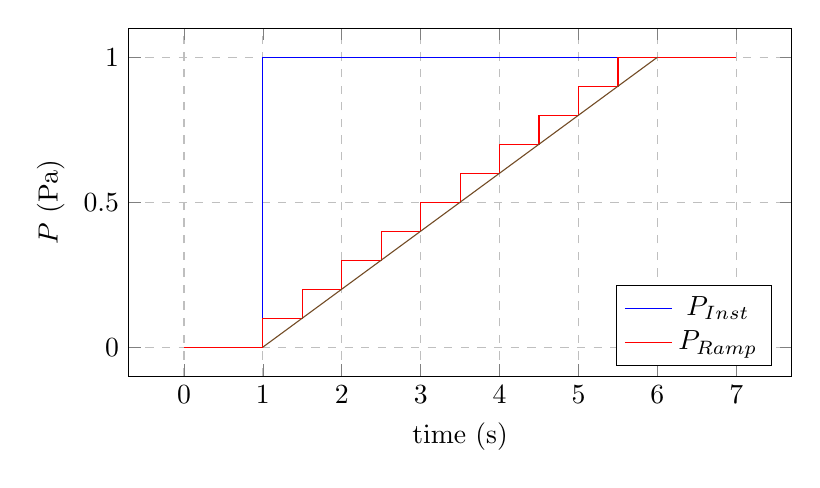
\begin{tikzpicture}
        \begin{axis}[width = 10cm, height = 6cm,
            xlabel = {time (s)},
            ylabel = {\(P\) (Pa)},
            %xmin = 0, xmax = 200000,
            legend pos = south east,
            ymajorgrids = true,
            xmajorgrids = true,
            grid style = dashed,
            ]

            \addplot+[no marks] coordinates{(0,0)(1,0)(1,1)(7,1)};
            \addlegendentry{\(P_{Inst}\)}

            \addplot+[no marks] coordinates{(0,0)(1,0)(1,0.1)(1.5,0.1)(1.5,0.2)(2,0.2)(2,0.3)(2.5,0.3)(2.5,0.4)(3,0.4)(3,0.5)(3.5,0.5)(3.5,0.6)(4,0.6)(4,0.7)(4.5,0.7)(4.5,0.8)(5,0.8)(5,0.9)(5.5,0.9)(5.5,1)(6,1)(7,1)};
            \addlegendentry{\(P_{Ramp}\)}

            \addplot+[no marks] coordinates{(1,0)(6,1)};
        \end{axis}
    \end{tikzpicture}
    \caption{Neumann Boundary Condition for pressure, $t_0$ = 1s , $t_f$ = 6s , $dt$ = 0.5s}
    \label{PressureInstRamp}
\end{figure}

\subsubsection{Nodal forces}
The keyword \textbf{*BOUNDARY, TYPE=FORCE} will be followed by the t0, tf, and the amount of force F in the next line separated by commas. In the next lines, the list of nodes should be provided together with the specific factors of F in each following column that corresponds to the directions of the force (column 1-x, column 2-y, column 3-z).

Example:
\begin{lstlisting}
*BOUNDARY, TYPE=FORCE
0, 0.1, 1000
15, 0,  1, 0
30, 0,  1, 0
45, 0,  1, 0
60, 0,  1, 0
75, 0,  1, 0
90, 0,  1, 0
105, 0,  1, 0
120, 0, 1, 0
*BOUNDARY, TYPE=FORCE
0.1, 0.2, -1000
15, 0.25,  1, 0
30, 0.25,  1, 0
45, 0.25,  1, 0
60, 0,  1, 0
75, 0,  1, 0
90, 0,  1, 0
105, 0,  1, 0
120, 0, 1, 0
\end{lstlisting}

For node 15, a force of 1000 will be applied in the y direction from 0 to 0.1, and from 0.1 to 0.2 a load of -1000*0.25 in the x direction and -1000 in the y direction.

\subsubsection{Pressure}
The application of pressure is not straightforward. It is available in 2D and 3D. The application is as follows (see \citep{zienkiewicz:2014}):
\begin{equation}
f_p=\int_{\partial\Omega_c}N_ap\mathbf{n}d\Omega
\end{equation}
where p is the pressure (which is applied incrementally or progressively), $N$ is the shape function and $\mathbf{n}$ is the normal vector at the current configuration. Using Nanson's formula, the equation in the reference configurations reads:
\begin{equation}
f_p=\int_{\partial\Omega_0}N_aJp\mathbf{F}^{-T}\mathbf{n}_0d\Omega_0
\end{equation}
where this equation should be integrated numerically.

The keyword \textbf{*BOUNDARY, TYPE=PRESSURE INST} is needed for an instant and constant pressure and the keyword \textbf{*BOUNDARY, TYPE=PRESSURE RAMP} is needed to make a progressive ramp between t0 and tf.

\begin{figure}[htb]
    \centering
    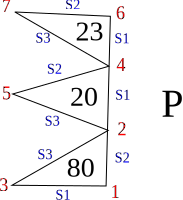
\includegraphics[width=0.3\textwidth]{imgs/UserManual/pressure.pdf}
    \caption{Pressure application in 2D}
    \label{fig:pressure}
\end{figure}

\subsubsection*{In 2D, pressure on edges}
In order to apply the pressure, the edges on which the pressure will be applied should be identified, see Figure \ref{fig:pressure}. The pressure P will be applied to that face of the domain. In that region we have the triangular elements 80 (with the nodes: 3, 1 and 2), 20 (with the nodes: 2, 4 and 5) and 23 (with the nodes: 4, 6 and 7), all of them anti-clock wise. The advantage of Abaqus is that the edges of the triangles are always defined going from the first node of the element to the last one, see Figure \ref{fig:pressure}. So, for the elements 80, 20 and 23, the subelements S1, S2 and S3 are arranged as shown in the figure. Therefore, to apply the pressure P, it should be applied to the subElement S2 of element 80, and subelements S1 of 20 and 23. The application of the pressure P shown in Figure \ref{fig:pressure} reads:
\begin{lstlisting}
*BOUNDARY, TYPE=PRESSURE INST
t0, tf, P, 1
20
23
*BOUNDARY, TYPE=PRESSURE INST
t0, tf, P, 2
80
\end{lstlisting}

 where in the first line, t0 is the initial time to apply the pressure, tf the final time, P the amount of pressure and the last value corresponds to the surface of the elements listed below.

 \begin{figure}[htb]
    \centering
    \includegraphics[width=0.6\textwidth]{imgs/UserManual/3D_pressure.pdf}
    \caption{Pressure application in 3D}
    \label{fig:pressure3D}
\end{figure}

 \subsubsection*{3D, pressure on surfaces}

 In order to apply the pressure, the surfaces on which the pressure will be applied should be identified, see Figure \ref{fig:pressure3D}. The pressure P will be applied to that face of the domain. In that region we have the tetrahedron elements E1 (with the nodes 4, 5, 2 and 3) and E2 (with the nodes: 3, 5, 2 and 1), all of them anti-clock wise. The advantage of Abaqus is that the edges of the tetrahedrons are always defined in a specific order, see Figure \ref{fig:pressure3D}. So, for the elements E1 and E2, the subelements S1, S2, S3 and S4 are arranged as shown in the figure. Therefore, to apply the pressure P on the grey area, it should be applied to the subElement S3 of element E1, and subelement S1 of E2. The application of the pressure P shown in Figure \ref{fig:pressure3D} reads:
\begin{lstlisting}
*BOUNDARY, TYPE=PRESSURE INST
t0, tf, P, 1
2
*BOUNDARY, TYPE=PRESSURE INST
t0, tf, P, 3
1
\end{lstlisting}

 where in the first line, t0 is the initial time to apply the pressure, tf the final time, P the amount of pressure and the last value corresponds to the edge of the elements listed below.

 \subsubsection{Traction boundary conditions}

 The keyword \textbf{*BOUNDARY, TYPE=TRACTION INST} is needed for an instant traction and the keyword \textbf{*BOUNDARY, TYPE=TRACTION RAMP} is needed to make a progressive ramp between t0 and tf.

 The application of the traction boundary condition is available in 2D and 3D. The support is defined in a similar way to that considered in the case of the pressure boundary condition. The application of a traction (Tx, Ty, Tz) on the grey area in Figure \ref{fig:pressure3D} reads
 \begin{lstlisting}
 *BOUNDARY, TYPE=TRACTION INST
 t0, tf, Tx, Ty, Tz, 1
 2
 *BOUNDARY, TYPE=TRACTION INST
 t0, tf, Tx, Ty, Tz, 3
 1
 \end{lstlisting}

 \subsubsection{Contact}

 The application of contact is not straightforward. The radius of the area of the contact, a, and the friction coefficient $\mu$ must be specified in the input file.

 \begin{equation}
f_p=\int_{\partial\Omega_c}N_ap\mathbf{n}d\Omega
\end{equation}
 \begin{equation}
f_t=\int_{\partial\Omega_c}N_at\mathbf{n_{t}}d\Omega,
\end{equation}
where p and t are respectively the inhomogeneous normal and tangential pressure (which are applied incrementally or progressively), $N$ is the shape function and $\mathbf{n}$ is the normal vector at the current configuration. Using Nanson's formula, the equation in the reference configurations reads:

\begin{equation}
f_p=\int_{\partial\Omega_0}N_aJp\mathbf{F}^{-T}\mathbf{n}_0d\Omega_0
\end{equation}
\begin{equation}
f_p=\int_{\partial\Omega_0}N_aJt\mathbf{F}^{-T}\mathbf{n_{t}}_0d\Omega_0.
\end{equation}

\subsubsection{Extra dof - Neumann flux}

The keyword \textbf{*HERTZIAN CONTACT} will be followed by start and end times --t0 and tf-- and the total normal and tangential forces applied in the area of contact, the friction coefficient, the radius of contact and the index of the subsurface in the next line separated by commas. In the next line, the coordinates of the center of the contact is specified. In the next lines, the elements should be listed line by line.

Example:
\begin{lstlisting}
*HERTZIAN CONTACT
0,1,800000,200000,0.3,3,3
0,0,2
1
2
3

\end{lstlisting}

\subsubsection{Extra dof - Surface heat flux}

The keyword \textbf{*FLUX EXTRADOF, TYPE=HEAT INST} will be followed by start and end times --t0 and tf--, the values of the components of the diagonal of the matrix that define the surface heat flux $\bm{q_0}$ (the third components is equal to zero for a 2D case) in the next lines separated by commas and finally, the surface on which the heat flux will be applied. In the next lines, the elements should be listed line by line.

Example:
\begin{lstlisting}
*FLUX EXTRADOF, TYPE=HEAT INST
0, 200, 802, 802, 0, 1
50
\end{lstlisting}
Notice that different sign nomenclature is used in 2D and 3D. A surface heat flux acting inwards the surface has to be defined as positive for 2D, and negative for 3D.

\subsubsection{Extra dof - Volumetric heat flux}

To define constant volumetric heat flux during the time interval $[t_0, t_f]$ in a group of elements, the keyword \textbf{*FLUX EXTRADOF, TYPE=VOLUMETRIC HEAT FLUX} will be followed by start and end times --t0 and tf--, and the prescribed volumetric heat flux  per volume $r$. In the next lines, the elements should be listed line by line.

The heat flux can be also defined as a moving Gaussian source by the keyword \textbf{*FLUX EXTRADOF, TYPE=GAUSSIAN VOLUMETRIC HEAT FLUX}. For a heat source whose initial position $(x_0,y_0,z_0)$ moving at a velocity $(v_x, v_y, v_z)$, the current flux reads
\begin{eqnarray}
	&&r = q_{max}\exp(-R)\,, \\
	&& \text{ where } R = (\frac{x-x_c}{a})^2 + (\frac{y-y_c}{b})^2+(\frac{z-z_c}{c})^2 \\
	&&\text{ with } x_c = x_0+v_x(t-t_0),  y_c = y_0+v_y(t-t_0),  \text{ and }  z_c = z_0+v_z(t-t_0),  
\end{eqnarray}
In the input file, this boundary condition is defined as
\begin{lstlisting}
	*FLUX EXTRADOF, TYPE=GAUSSIAN VOLUMETRIC HEAT FLUX
	t0, tf, qmax, x0, y0, z0, vx, vy, vz, a, b, c
\end{lstlisting}


\subsubsection{Extra dof - Surface convection}

The keyword \textbf{*FLUX EXTRADOF, TYPE=CONVECTION} will be followed by start and end times --t0 and tf--, the film coefficient $h$, the sink temperature $\theta^0$ and finally, the surface on which the heat flux will be applied. In the next lines, the elements should be listed line by line.

\subsubsection{Extra dof - Radiation}
The keyword \textbf{*FLUX EXTRADOF, TYPE=RADIATION} will be followed by start and end times --t0 and tf--, the radiation constant $A$, which is calculated as emissivity times the Stefan-Boltzmann constant($5.67 \times 10^{-8}\quad W/m^2 K^4$), the sink temperature $\theta^0$ and finally, the surface on which the heat flux will be applied. In the next lines, the elements should be listed line by line. It should be noted that the implementation of radiation has been carried out considering kelvin as a temperature scale.
\subsection{Initial conditions}\label{secInitialConditions}
\textit{Initial conditions} is an option to initialise the value of the  extradof variables, i.e. normalised voltage, temperature etc. If this is not defined in the input file, the variables are initialised to zero.

The keyword \textbf{*INITIAL CONDITIONS EXTRADOF} will be followed by the initial value of each extradof, each separated by a comma.
Example
\begin{lstlisting}
*INITIAL CONDITIONS EXTRADOF
273
\end{lstlisting}

Note that these must follow the same order that is used in the definition of materials. That means if we define:
\begin{lstlisting}
*ExtraDof
*FHNelec
1, 0, 0, 1, 0, 0.4, 0.4, 0.01, 0.085, 0
*ExtraDof
*Temperature
0, 0, 401, 0, 0, 0, 0
 ...
\end{lstlisting}
The first extradof variable will be normalised voltage and the second one temperature.
In addition, this option must be defined before \textbf{*MATERIAL}.

\subsection{Materials}\label{secMaterials}
All new constitutive models will inherit from the parent class constitutiveModels, see Figure \ref{fig:ClassConsMod}. The theory which the corresponding constitutive model is based on should be cited in the doxygen file. To implement a new law, some virtual functions specifying in \textit{constitutiveModels.h} that MUST be implemented by the user.

\begin{figure}[htb]
   ClassConsMod \centering
    \includegraphics[scale=0.5]{imgs/UserManual/classconstitutiveModels.pdf}
    \caption{Class constitutive models inheritance diagram}
    \label{fig:}
\end{figure}

In terms of materials, each of them should be defined with the keyword \textbf{*MATERIAL, name=RegionX} where regionX is the name for the corresponding region. In the next line, the density should be specified with the keyword \textbf{*Density} with its value in the next line. In the next line the type of material should be specified. The constitutive models available in \textit{MuPhiSim} are the following:
\begin{enumerate}

\item Area growth, keyword \textbf{*AreaGrowth}. Next line, the Young's modulus, the Poisson's ratio and the growth multiplier. The perpendicular direction to the growth plane is given in the constitutive model.
\item FitzHugh-Nagumo (FHN), electrophysiology, keyword \textbf{*ExtraDof}. This constitutive model is linked with \textit{Electrophysiology.} analysis. Next line, \textbf{*FHNelec}.  The mechanical coupling is obtained using the keyword \textbf{*FHNelecCoupling} in which the constitutive model depends on the deformation gradient. Only one line is needed to define the model: $a_{o/x}$, $a_{o/y}$, $a_{o/z}$, $D_{iso}$, $D_{ani}$, $a_{elec}$, $b$, $\varepsilon$, $\Phi_{equi}$, $I$ where: \\
Axonal direction: $n_o = \{a_{o/x}, a_{o/y}, a_{o/z}\}$\\
Conductivity tensor, defined by its isotropic and anisotropic components: $D_{iso}$ and $D_{ani}$\\
Activation parameters: $a_{elec}$, $b$\\
Time-scale difference: $\varepsilon$\\
Equilibrium potential: $\Phi_{equi}$\\
stimulus current: $I$\\
Everything must be separated by commas.
\item Temperature, keyword \textbf{*ExtraDof}. This constitutive model can be linked to uncoupled heat transfer analysis (\textit{Heat}) or with fully coupled thermal-stress analysis (\textit{Thermomechanics.}). Therefore, in next line, the user has to specify \textbf{*Temperature} for uncoupled analysis or \textbf{*TemperatureCoupling} for coupling analysis.
Only one line is needed to define the model: $C_0$, $C_1$, $k_0$, $k_1$, $\theta_{ini}$, $\theta_{ref1}$, $\theta_{ref2}$ where:  \\
Specific heat capacity at constant volume, reference temperature: $C_0$\\
Parameters that described the temperature-dependence of $C$: $C_1$ and $\theta_{ref1}$\\
Heat flux per volume: $r$\\
Material conductivity (current configuration) at reference temperature: $k$ \\
Parameters that described the temperature-dependence of $k$: $k_1$ and $\theta_{ref2}$\\
%Direction of conductivity anisotropy: $n=\{n_{1}, n_{2}, n_{3}\}$\\
Reference temperature to describe the temperature-dependence of $\alpha$ (not implemented yet, just used for coupling analysis): $\theta_{ini}$
\\
Everything separated by commas.
\item Fiber growth, keyword \textbf{*FiberGrowth}. Next line, the Young's modulus, the Poisson's ratio and the growth multiplier. The direction of growth is given in the constitutive model.
\item Linear elastic, keyword \textbf{*Linear-Elastic}. Next line, the Young's modulus and the Poisson's ratio are defined. 2D plane stress/ plane strain can be defined by the keyword:  \textit{PlaneStress}/ \textit{PlaneStrain}) after two material parameters.
\item Finite strain $J_2$ plasticity model, keyword  \textbf{*J2plasticityFiniteStrain}. The model considered the bi-logarithmic elastic potential\footnote{For the model details, refer to Nguyen, V. D., \& Noels, L. (2014). Computational homogenization of cellular materials. International Journal of Solids and Structures, 51(11-12), 2183-2203 .}. The elastic strain is defined by $\mathbf{E}^e = \log\sqrt{\mathbf{F}^{eT}\cdot \mathbf{F}^{e}}$ where $\mathbf{F}^{e}$ is the elastic deformation gradient. To approximate the logarithmic tensorial operator, the Taylor series is used instead of using the direct tensorial evaluation. Next line, the Young's modulus, the Poisson's ratio, the order of the Taylor series must be defined.The next line, a hardening law is provided. Three different laws are available: 
\begin{itemize}
    \item The keyword LinISO for linear hardening, ie $\sigma_y =\sigma_y^0+ H p$ where $\sigma_y^0$ is the initial yield stress, $p$ is the equivalent plastic strain and  $H$ is a constant. To deine a finite strain $J_2$ plasticity model using this hardening law
    \begin{lstlisting}[mathescape=true]
*J2plasticityFiniteStrain
E,$\nu$,order
LinISO,$\sigma_y^0$,H
\end{lstlisting}
    \item The keyword SwiftISO for Swift hardening, \emph{i.e.} $\sigma_y =\sigma_y^0\left(1+ p/p_0 \right)^n$ where $\sigma_y^0$ is the initial yield stress, $p$ is the equivalent plastic strain and  $p_0$, $n$ are constants. To deine a finite strain $J_2$ plasticity model using this hardening law
    \begin{lstlisting}[mathescape=true]
*J2plasticityFiniteStrain
E,$\nu$,order
SwiftISO,$\sigma_y^0$,$p_0$,$n$
\end{lstlisting}   
\item The keyword VoceISO for Voce hardening, \emph{i.e.} $\sigma_y =\sigma_y^0+ K\left[1-\exp\left(Cp\right) \right]$ where $\sigma_y^0$ is the initial yield stress, $p$ is the equivalent plastic strain and $K$, $C$ are constants. To define a finite strain $J_2$ plasticity model using this hardening law
    \begin{lstlisting}[mathescape=true]
*J2plasticityFiniteStrain
E,$\nu$,order
VoceISO,$\sigma_y^0$,$K$,$C$
\end{lstlisting}   
\end{itemize}
It is noted that the \emph{order} should be an odd number, \emph{e.g.} a value equal to 11 should be a good choice.
\item Hyperelasticity, keyword \textbf{*HyperElastic, Type} where \textbf{Type} is directly replaced by the hyperelastic material:
\begin{itemize}
    \item \textbf{Neo-Hookean}, the Young's modulus and the Poisson's ratio should be defined on the next line.
    \item \textbf{St-Venant-Kirchhoff}, the Young's modulus and the Poisson's ratio should be defined on the next line. Equivalent to linear elastic for small deformations. 2D plane stress/ plane strain hardcoded (must be defined in the input file with the keyword:  \textit{PlaneStress}/ \textit{PlaneStrain}). 3D Isotropic material.\\ *In addition, this constitutive model includes an activation criterion to activate elements which internal variable is greater than the simulation time at that moment. This option is only available using the keyword  \textbf{*ACTIVATION} and defining the activation time as an internal variable using \textbf{*INITINTVARS}.
   \item \textbf{St-Venant-Kirchhoff-ThermoMechanics}. This constitutive model is designed as a wrapper to couple Hyper Elastic St-Venant-Kirchhoff model with a thermomechanical couling term. The Young's modulus, the Poisson's ratio, thermal expansion and initial temperature (this model assumes that reference temperature for the thermal expansion is equal to the initial temperature) should be defined on the next line. Equivalent to linear elastic for small deformations. 2D plane stress/ plane strain hardcoded. 3D Isotropic material. This constitutive model is just used for \textit{Thermomechanics} analysis. \\ *In addition, this constitutive model includes an activation criterion to activate elements which internal variable is greater than the simulation time at that moment. This option is only available using the keyword  \textbf{*ACTIVATION} and defining the activation time as an internal variable using \textbf{*INITINTVARS}.

\end{itemize}
\item Volumetric growth, keyword \textbf{*IsoMorphoGrowth}. Next line, the Young's modulus, the Poisson's ratio and the growth multiplier.
\item Viscoelastic, keyword \textbf{*ViscoElastic}. You will need 4 lines to define the model:\\
Bulk modulus: $K$\\
Number of branches in the generalised maxwell model\\
Shear moduli for all the branches: $\mu_\infty$, $\mu_1$ ...\\
Viscosities for all the branches: $\eta_1$, $\eta_2$...
\item Viscoelastic Growth, keyword \textbf{*ViscoGrowth}. You will need 5 lines to define the model:\\
Bulk modulus: $K$\\
Number of branches in the generalised maxwell model\\
Shear moduli for all the branches: $\mu_\infty$, $\mu_1$ ...\\
Viscosities for all the branches: $\eta_1$, $\eta_2$...\\
Growth multiplier of the isomorpho growth used in the coupling.
\item Viscoelastic fibre growth due to polymerisation, keyword \textbf{*ViscoMechAxialGrowth}. You will need 5 lines to define the model:\\
Bulk modulus: $K$\\
Number of branches in the generalised maxwell model\\
Shear moduli for all the branches: $\mu_\infty$, $\mu_1$ ...\\
Viscosities for all the branches: $\eta_1$, $\eta_2$...\\
The initial growth multiplier, the polymerisation rate, the depolymerisation rate, the density of cytoskeletal filaments, and finally the whole vector of the direction of growth, everything separated by commas.
\item Viscoelastic fibre growth due to polymerisation with contractility, keyword \textbf{*ViscoMechContractAxialGrowth}. You will need 5 lines to define the model: \\
Bulk modulus: $K$\\
Number of branches in the generalised maxwell model\\
Shear moduli for all the branches: $\mu_\infty$, $\mu_1$ ...\\
Viscosities for all the branches: $\eta_1$, $\eta_2$...\\
The initial growth multiplier, the polymerisation rate, the depolymerisation rate, the density of cytoskeletal filaments, the contractility rate, the stress threshold for contractility, and finally the whole vector of the direction of growth, everything separated by commas.

\item Volumetric growth as a consequence of variations in the deformation gradient (mechanical growth). There are two type of functions: the virtual ones inherited from the general constitutive law (they MUST be implemented by the user), and the particular ones that the user wants to implement for their convenience. Keyword \textbf{*VolMechDrivenGrowth}, Not yet implemented in \textit{InputFile.cpp}.

\item Stochastic Kirchhoff-St-Venant model. In addition to the Hyperelastic St-Venant-Kirchhoff constitutive model, the Young's modulus and Poisson's ratio can be random variables. For the moment, they only exhibit a Gaussian distribution and are space-independent. To activate the stochastic analysis, the keyword \textbf{*Stochastic} must be specified before \textbf{*HyperElastic}. The order of the expansion needs to be specified after the keyword \textbf{*Order}. Then the randomness of variables are specified using this convention: the first number relates to which variable is supposed to be random (1 for Young's modulus and 2 for Poisson's ratio). Next the number of functions used to described this random variable. Finally, the ratio of the standard variation to the mean value is indicated for each of these functions. We take the following file as an example:
\begin{lstlisting}
*Stochastic
*HyperElastic, St-Venant-Kirchhoff
1E7, 0.3
*ORDER
3
1, 1, 0.1
2, 1, 0.1
*POLYNOMIAL
CHAOS
\end{lstlisting}
In that case the Young's modulus is a Gaussian variable of mean 1E7 and standard deviation of 1E7 times 0.1. The Poisson's modulus is a Gaussian variable of mean 0.3 and standard deviation of 0.3times 0.1.
The keyword \textbf{CHAOS} can be replaced by \textbf{Haar} if one needs a discontinuous polynomial expansion.
\item Thermomechanical model for 3D printing simulation, keyword \textbf{*3DPrinting-St-Venant-Kirchhoff-Thermoelasticity}. This constitutive model is St-Venant-Kirchhoff model with a thermomechanical coupling term and temperature-dependent properties. The model has been developed to capture the physics of a selective laser melting process. This 3D printing technology starts with powder as a starting material. A laser melts the powder along a predefined path, changing the material from powder to liquid, and to solid when the laser is far enough away. Thermal strains are neglected for powder and liquid phase. Finally, under the assumption of an open system, new powder is always filling the molten pool. This model considers a new reference configuration when the material turns to liquid, being an element in a stress-free configuration the first time that this turns from powder to liquid, at the same time that a change from $\rho_{powder}$ to  $\rho_{liquid}$ is produced (see fig.  \ref{3DprintingTheory} and for more information subsection \ref{3Dprinting-model}).
\begin{figure}[h!]
    \centering
    \includegraphics[scale=0.5]{imgs/UserManual/Theory2.pdf}
    \caption{Description of the different combination of phases}
    \label{3DprintingTheory}
\end{figure}


You will need only one line to define the model (Everything separated by commas): $\rho_{newConf}$, $\rho_{transition}$, $E_{P_{ref}}$,
$E_{PL}$, $E_{S_{ref}}$, $E_{{SL}_1}$, $E_{{SL}_2}$, $\upsilon_{S_{ref}}$, $\upsilon_{SL}$, $\kappa_{SL}$, $\theta_{sigMidpoint}$, $\alpha_{solid}$, $\theta_{ref}$, $\theta_{SL}$ $\theta_{liq}$ (being \textit{P}: powder, S: solid, \textit{PL}: transition powder-liquid, \textit{SL}: transition solid-liquid, \textit{sigMidpoint}: value of the sigmoid's function midpoint) where (see Figure \ref{fig:3D-printingModels}):  \\

   \begin{equation*}
    E (GPa)=\left\{ \begin{array}{lcc}
    P:\quad E_{P_{ref}} + \frac{E_{PL}}{1 +\exp(-\kappa_{SL} (\theta -\theta_{sigMidpoint}))} \\ \\ S-L: \quad \begin{array}{lcc}
    E_{S_{ref}}  + \frac{E_{SL_1} }{1 +\exp(-\kappa_{SL} (\theta -\theta_{sigMidpoint}))} + E_{SL_2}  (\theta - \theta_{SL}) & if & \theta \leq \theta_{SL}\\
    E_{S_{ref}} +  \frac{E_{S_1}}{1 +\exp(-\kappa_{SL} (\theta -\theta_{sigMidpoint}))}& if & \theta> \theta_{SL}
    \end{array}
    \end{array}
    \right.
    \end{equation*}
    
    \begin{equation*}
    \upsilon (-)=
     \upsilon_{S_{ref}} + \frac{\upsilon_{SL}}{1 +\exp(-\kappa_{SL} (\theta -\theta_{sigMidpoint}))}
    \end{equation*}
    
    \begin{equation*}
    \alpha (1/K)= \frac{\alpha_{S}}{1 +\exp(\kappa_{SL} (\theta -\theta_{sigMidpoint}))}
    \end{equation*}


This constitutive model is just used for \textit{Thermomechanics} analysis.
\\The material phase (Powder = 0, Liquid = 1 and Solid= 2), is modelled through a internal variable ($1^{st}=$activation time, $2^{nd}=$activation state, $3^{rd}=$material phase, $4^{th}=E(\theta)$, $5^{th}=\upsilon(\theta)$, $6^{th}=$ thermal stretch ratio) as:
\begin{equation*}
    intVarsCurr[2]=\left\{ \begin{array}{lcc}
    0  & if & intVarsPrev[2]=0 \; \& \; T\leq \theta_{Liquid}\\
    1 & if & intVarsPrev[2]\geq0 \; or \; T> \theta_{Liquid}\\
    2 & if & intVarsPrev[2]\geq1 \; or \; T\leq \theta_{Liquid}
    \end{array}
    \right.
    \end{equation*}

 *In addition, this constitutive model includes an activation criterion to activate elements which internal variable is greater than the simulation time at that moment. This option is only available using the keyword  \textbf{*ACTIVATION} and defining the activation time as an internal variable using \textbf{*INITINTVARS}.

\item Temperature model for 3D printing simulation, keyword \textbf{*3DprintingTemperature}. This constitutive model has temperature-dependent properties. To be used in combination with the  mechanical coupling is necessary to use the keyword \textbf{*3DprintingTemperatureCoupling} (to be used in combination with \textbf{*3DPrinting-St-Venant-Kirchhoff-Thermoelasticity}). You will need only one line to define the model (Everything separated by commas): $C_{S_{ref}}$,
$C_{SL_1}$, $C_{SL_2}$, $L_{\_PL1}$, $L_{\_PL2}$, $L_{\_PL3}$, $L_{\_SL1}$, $L_{\_SL2}$, $L_{\_SL3}$, $k_{P_{ref}}$, $k_{PL_1}$, $k_{S_{ref}}$, $k_{SL_1}$, $k_{SL_2}$, $k_{SL_3}$, $\kappa_{SL}$, $\theta_{SigMidpoint}$, $\theta_{ref}$, $\theta_{powder}$ $\theta_{SL}$, $\theta_{liq}$ (being \textit{P}: powder, S: solid, \textit{PL}: transition powder-liquid, \textit{SL}: transition solid-liquid, \textit{sigMidpoint}: value of the sigmoid's function midpoint)
where (see Figure \ref{fig:3D-printingModels}):

 \begin{equation*}
    C (J/Kkg)=\left\{ \begin{array}{lcc} P:
    \begin{array}{lcc}
    C_{S_{ref}}+ \frac{C_{S_1}}{1 +\exp(-\kappa_{SL} (\theta -\theta_{sigMidpoint}))} & if & \theta\leq \theta_{ref}\\
    C_{S_{ref}}+ \frac{C_{S_1}}{1 +\exp(-\kappa_{SL} (\theta -\theta_{sigMidpoint}))} + C_{S_2} (\theta - \theta_{ref})  & if & \theta_{ref}\geq \theta\leq\theta_{powder}\\
    -L_{PL_1} \theta^2 + L_{PL_2} \theta -L_{PL_3}  & if & \theta_{powder}> \theta < \theta_{liq} \\
    C_{S_{ref}}+ \frac{C_{S_1} }{1 +\exp(-\kappa_{SL} (\theta -\theta_{sigMidpoint}))} & if & \theta\geq \theta_{liq}
     \end{array}\\ \\
     S-L:\begin{array}{lcc}
    C_{S_{ref}}+ \frac{C_{S_1}}{1 +\exp(-\kappa_{SL} (\theta -\theta_{sigMidpoint}))} & if & \theta\leq \theta_{ref}\\
    C_{S_{ref}}+ \frac{C_{S_1} }{1 +\exp(-\kappa_{SL}  (\theta -\theta_{sigMidpoint}))} + C_{S_2} (\theta - \theta_{ref})  & if & \theta_{ref}\geq \theta\leq\theta_{SL}\\
    -L_{SL_1} \theta^2 + L_{SL_2}  \theta -L_{SL_3}  & if & \theta_{SL}> \theta <\theta_{liq} \\
    C_{S_{ref}}+\frac{C_{S_1} }{1 +\exp(-\kappa_{SL} (\theta -\theta_{sigMidpoint}))} & if & \theta\geq \theta_{liq}
    \end{array}
    \end{array}
    \right.
    \end{equation*}
    
    \begin{equation*}
    k (W/mK)=\left\{ \begin{array}{lcc} P:
    k_{P_{ref}} + \frac{k_{P_1}}{1 +\exp(-\kappa_{SL} (\theta -\theta_{sigMidpoint}))}  \\ \\
    S-L: \begin{array}{lcc}
    k_{S_{ref}}+ \frac{k_{S_1}}{1 +\exp(-\kappa_{SL} (\theta -\theta_{sigMidpoint}))} & if & \theta\leq \theta_{ref}\\
    k_{S_{ref}}+ \frac{k_{S_1}}{1 +\exp(-\kappa_{SL} (\theta -\theta_{sigMidpoint}))} + k_{S_2} (\theta - \theta_{ref})  & if & \theta_{ref}\geq \theta\leq\theta_{liq}\\
    k_{S_3}+ \frac{k_{S_2}}{1 +\exp(-\kappa_{SL} (\theta -\theta_{sigMidpoint}))} & if & \theta\geq \theta_{liq}
    \end{array}
    \end{array}
    \right.
    \end{equation*}

    The  value of some material properties, temperature-dependent, can be analysed through the internal variable ($intVar[\_intVarsSizeTemp]=$conductivity, $intVar[\_intVarsSizeTemp+1]=$specific heat, $intVar[\_intVarsSizeTemp+2]=$ density).
    
    \begin{figure}[H]
    \centering
    \includegraphics[scale=0.5]{imgs/UserManual/MaterialProperties3DPrinting.pdf}
    \caption{3D printing constitutive models: a) and b) material properties of 3DPrintingTemperature model; c), d) and e) material properties of 3DPrinting-St-Venant-Kirchhoff-Thermoelasticity model}
    \label{fig:3D-printingModels}
\end{figure}
\end{enumerate}


The list of elements for the specific material should be provided with the keyword  \textbf{*List of Elements}, with one label of the element per line. You can also define a bounding box with the keyword \textbf{*Bounding box} and then list the corner nodes of the box. All of the nodes inside the box will be selected. \textbf{THIS FEATURE IS NOT YET IMPLEMENTED}.

Example:
\begin{lstlisting}

*FLUX EXTRADOF, TYPE=CURRENT INST
0, 5, 0.3
1
2
*FLUX EXTRADOF, TYPE=CURRENT INST
100, 110, 0.2
40
41
42
43
\end{lstlisting}
Finally, to define the initial value of a specific internal variable, we must provide the element in whose GPs we want to define an internal variable followed by the position and the value of the internal variable. All elements defined here must be contained in the \textbf {* List of Elements} previously defined for the material.
Example:
\begin{lstlisting}
*INITINTVARS
1, 1, 0
2, 1, 0.2
3, 1, 0.4
4, 1, 0.6
\end{lstlisting}
Please note that all input files must be ended with the keyword \textbf{*END} at the end of the file. This is the list of input files provided with the program to illustrate a typical input file for \textit{MuPhiSim}

\subsection{Data extraction}

The numerical results often need to be extracted, e.g. displacement at a point, reaction force at a boundary, total elastic energy in the problem, maximal stress in the model, \emph{etc.} This code provides different possibilities for data extraction. The extracted data is written in the current folder under the \textbf{.csv} files specifying a value of a quantity over time, e.g.
\begin{lstlisting}
Time;Value
...
...
\end{lstlisting}

The data at nodes can be extracted using \textbf{*EXTRACTION, NODE}. This block is defined as follows
\begin{lstlisting}
*EXTRACTION, NODE
prefix,quantity,Operation,comp
n1
n2
...
nN
\end{lstlisting}
In this block, one has
\begin{itemize}
	\item \textbf{prefix}: a string is defined by user and used as the first part of the file name.
	\item \textbf{quantity}: a quantity name must be chosen between \textbf{Unknown} for unknown field, \textbf{InternalForce} for internal force or \textbf{ExternalForce} for external force.
	\item \textbf{Operation}: an operation must be chosen between \textbf{Mean}, \textbf{Max}, \textbf{Min}, \textbf{Sum}, and \textbf{Rough}. When \textbf{Rough} is used, the output file includes all values at all nodes, where each value of each node is provided by a column.
	\item \textbf{comp}: the component to be extracted.
	\item \textbf{n1, n2, ..., nN}: list of nodes
\end{itemize}
Some useful cases:
\begin{itemize}
	\item Extract the displacement following y of node 100
	\begin{lstlisting}
	*EXTRACTION, NODE
	node10Disp,Unknown,Mean,1
	10
	\end{lstlisting}
	\item Extract the total internal force following y on the boundary whose nodes are 10, 20, 30:
	\begin{lstlisting}
	*EXTRACTION, NODE
	node10Disp,InternalForce,Sum,1
	10
	20
	30
	\end{lstlisting}
\end{itemize}

The data at GPs can be extracted using \textbf{*EXTRACTION, ELEMENT}. This block is defined as follows
\begin{lstlisting}
*EXTRACTION, ELEMENT
prefix,quantity,Operation
e1
...
eN
\end{lstlisting}
In this block, one has
\begin{itemize}
	\item \textbf{prefix}: a string is defined by user and used as the first part of the file name.
	\item \textbf{quantity}: a quantity name must be specify. Currently, deformation gradient components (\textbf{FXX, ..., FZZ}), stress components (\textbf{PXX, ..., PZZ}), \textbf{DEFO\_ENERGY, EXTERNAL\_ENERGY, KIN\_ENERGY} can be used.
	\item \textbf{Operation}: an operation must be chosen between \textbf{Mean}, \textbf{Max}, \textbf{Min}, and \textbf{Sum}.
	\item \textbf{e1, ..., eN}: list of elements
\end{itemize}
Some useful cases:
\begin{itemize}
	\item Extract the total energy of the model
	\begin{lstlisting}
	*EXTRACTION, ELEMENT
	totalEnergy,DEFO_ENERGY,Sum
	All
	\end{lstlisting}
	\item Extract the average of \textbf{FXX}
	\begin{lstlisting}
	*EXTRACTION, ELEMENT
	totalEnergy,FXX,Mean
	All
	\end{lstlisting}
	\item Extract maximum value of PYY over a groups of elements: 10, 20, 30:
	\begin{lstlisting}
	*EXTRACTION, NODE
	maxPyy,PYY,Max
	10
	20
	30
	\end{lstlisting}
\end{itemize}

%%%%%%%%%%%%%%%%%%%%%%%%%%%%%%%%%%%%%%%% CHAPTER 3 %%%%%%%%%%%%%%%%%%%%%%%%%%%%%%%%%%%%%%%%%%%%

\chapter{EXAMPLES DOCUMENTATION} \label{Chapter:examples}

\section{Test cases}

The following chapter aims at illustrating the contents of 16 examples of an input file for \textit{MuPhiSim}. For each example, the structure of elements, the solvers and the material are described through several figures where boundary conditions and a few values of stress or strain are shown for the purpose of a better understanding of the problem. There is a summary at the end of this document which presents the main data of each example. These 5 examples are built to study the following problems :

\begin{enumerate}
\item \texttt{example1.inp} Twisting of a beam made of FEM and MM elements
\item \texttt{example2.inp} Twisting of a beam made of a Visco-Growth model
\item \texttt{example3.inp} Vibration of a beam pulled up longitudinally and then transversely
\item \texttt{example4.inp} Stretching of a cell made of viscoMechContractAxialGrowth and viscoMechAxialGrowth models
\item \texttt{example5.inp} Flexion of an elastic bunny
\item \texttt{example6.inp} Electrophysiological model
\item \texttt{example7.inp} Artificial viscosity applied on the displacement of a piston with explicit solver
\item \texttt{example8.inp} Oscillation of a beam with an explicit solver after the application of a static pull
\item \texttt{example9.inp} Steady-state conduction heat transfer of a beam applying surface heat flux
\item \texttt{example10-11.inp} Transient conduction heat transfer cases
\item \texttt{example12.inp} Axial displacement of a beam due to heating
\item \texttt{example13.inp} Stochastic axial tip displacement of a 2D beam with random constitutive parameters
\item \texttt{example14.inp} Heat transfer analysis with progressively element activation
\item \texttt{example15.inp} 3D block with MM nodes and  partitioned into 4 regions to be assigned to different processors
\item \texttt{example16.inp} Transient heat problem with convection BC on a 2D plate
\end{enumerate}

\newpage
\subsection{Example 1 : \texttt{example1.inp}}
This input file presents a 3D beam made of both FEM and MM nodes/elements. The model used is HyperElastic, St-Venant-Kirchhoff. During the first second, a displacement of the face $z=0.6$ is computed by an Implicit Static solver. Then, at t = 1s, this face is released and the oscillations computed by an Implicit Dynamic solver for a two second period. In the case of parallel processing, the MM nodes/elements are assigned to one processor and the FEM nodes/elements are partitioned by METIS and allocated to the rest of the processors.
\medbreak
Figure \ref{ex1-BC} shows the initial configuration and the Dirichlet Boundary Conditions for the first solver. Figure \ref{ex1-disp} shows the beam at its maximum strain.

\begin{figure}[h!]
    \centering
    \includegraphics[scale=0.35]{imgs/Examples/ex1-BC.png}
    \caption{Initial configuration of the beam, example 1}
    \label{ex1-BC}
\end{figure}

\begin{figure}[h!]
    \centering
        \includegraphics[scale=0.35]{imgs/Examples/ex1-disp.png}
    \caption{Maximum deformation of the beam, example 1}
    \label{ex1-disp}
\end{figure}

\newpage
\subsection{Example 2 : \texttt{example2.inp}}
This input file presents a 3D beam made of FEM nodes and elements. The model used is ViscoGrowth. From t = 0 to t = 1s, a displacement of the face $z=600$ is computed by an Explicit solver.
\medbreak
Figure \ref{ex2-BC} shows the initial configuration and the Dirichlet Boundary Conditions. Figure \ref{ex2-def} shows the beam at the end of the study.

\begin{figure}[h!]
    \centering
    \includegraphics[scale=0.35]{imgs/Examples/ex2-BC.png}
    \caption{Initial configuration of the beam, example 2}
    \label{ex2-BC}
\end{figure}

Figure \ref{ex2-def} show the strain and Von Mises stress on distorted configuration of the beam.

\begin{figure}[h]
  \begin{center}
    \mbox{
      \subfigure[Strain ]{\scalebox{1}{\includegraphics[width=8cm]{imgs/Examples/ex2-disp.png}}}
      \quad
      \subfigure[Von Mises Stress]{\scalebox{1}{\includegraphics[width=8cm]{imgs/Examples/ex2-VMS.png}}} }
    \caption{Distorted configuration of example 2}
    \label{ex2-def}
  \end{center}
\end{figure}


\newpage
\subsection{Example 3 : \texttt{example3.inp}}
This input file presents a 2D beam made of FEM nodes and elements. The model used is HyperElastic, St-Venant-Kirchhoff. There are 4 solvers implemented here :
\begin{enumerate}
    \item From 0 to 1s : Implicit Static, the right side of the beam is pulled up.
    \item From 1 to 10s : Implicit Dynamic, the right side of the beam is released, the beam oscillates vertically.
    \item From 10 to 14s : Implicit Static, the right side of the beam is pulled to the right.
    \item From 14 to 20s : Implicit Dynamic, the right side of the beam is released, the beam oscillates horizontally.
\end{enumerate}
It has to be noted that the Dirichlet Boundary Conditions are incremental, therefore the beam is pulled to the right at $t=10s$ from a distorted configuration and not the initial.\\
Figures \ref{ex3t0} to \ref{ex3t14} show the distorted configuration of the beam before each solver.

\begin{figure}[h!]
    \centering
    \includegraphics[scale=0.19]{imgs/Examples/ex3t0.png}
    \caption{Initial configuration of the beam  -  $t=0s$}
    \label{ex3t0}
\end{figure}

\begin{figure}[h!]
    \centering
    \includegraphics[scale=0.35]{imgs/Examples/ex3t1.png}
    \caption{Distorted configuration of the beam  -  $U_{Y}$ field  -  $t=1s$}
    \label{ex3t1}
\end{figure}

\begin{figure}[h!]
    \centering
    \includegraphics[scale=0.18]{imgs/Examples/ex3t10.png}
    \caption{Distorted configuration of the beam  -  $U_{X}$ field  -  $t=10s$}
    \label{ex3t10}
\end{figure}

\begin{figure}[htbp]
    \centering
    \includegraphics[scale=0.35]{imgs/Examples/ex3t14.png}
    \caption{Distorted configuration of the beam  -  $U_{X}$ field  -  $t=14s$}
    \label{ex3t14}
\end{figure}

The nodal forces at the left side of the beam are saved in a .csv file. We are only registering the forces among $x$ direction during the first and the third solvers each 0.01s.

\newpage
~
\newpage
\subsection{Example 4 : \texttt{example4.inp}}
This input file presents a 2D beam made of FEM nodes and elements. There are two different regions named "membraneCortex" and "axonShaft" which are made of a ViscoMechContractAxialGrowth model (outline of the beam) and a ViscoMechAxialGrowth model (the centre of the beam) respectivelly. The solver used is Implicit Static between 0 and 2500s.

During the computation, pressure is progressively applied on the right side of the beam as presented on Figure \ref{ex4-BC}.

\begin{figure}[h!]
    \centering
    \includegraphics[scale=0.19]{imgs/Examples/ex4-BC.png}
    \caption{Initial configuration of the beam}
    \label{ex4-BC}
\end{figure}

Figures \ref{ex4Ux} to \ref{ex4VMS} show the distorted configuration of the beam at the end of the computation with $U_{X}$, $U_Y$ and $\sigma_{VMS}$ field.

\begin{figure}[h!]
    \centering
    \includegraphics[scale=0.35]{imgs/Examples/ex4Ux.png}
    \caption{Distorted configuration of the beam  -  $U_{X}$ field}
    \label{ex4Ux}
\end{figure}

\begin{figure}[h!]
    \centering
    \includegraphics[scale=0.35]{imgs/Examples/ex4Uy.png}
    \caption{Distorted configuration of the beam  -  $U_{Y}$ field}
    \label{ex4Uy}
\end{figure}

\begin{figure}[h!]
    \centering
    \includegraphics[scale=0.35]{imgs/Examples/ex4-VMS.png}
    \caption{Distorted configuration of the beam  -  $\sigma_{VMS}$ field}
    \label{ex4VMS}
\end{figure}

\newpage
~
\newpage
\subsection{Example 5 : \texttt{example5.inp}}
This input file presents a 2D bunny made of FEM nodes and elements. The model used is HyperElastic, St-Venant-Kirchhoff. From t=0-5s, a displacement of the nodes presented on Figure \ref{ex5-BC} is computed by an Implicit Static solver.

\begin{figure}[h!]
    \centering
    \includegraphics[scale=0.18]{imgs/Examples/ex5-BC.png}
    \caption{Initial configuration of the bunny}
    \label{ex5-BC}
\end{figure}

Figures \ref{ex5-disp} and \ref{ex5-VMS} show the distorted configuration of the bunny at the end of the computation with $||\overrightarrow{u}||_2$ and $\sigma_{VMS}$ field.

\begin{figure}[h!]
    \centering
    \includegraphics[scale=0.381]{imgs/Examples/ex5-disp.png}
    \caption{Distorted configuration of the bunny - $\left \lVert \protect\overrightarrow{u} \right \rVert_2$ field}
    \label{ex5-disp}
\end{figure}

\begin{figure}[h!]
    \centering
    \includegraphics[scale=0.37]{imgs/Examples/ex5-VMS.png}
    \caption{Distorted configuration of the bunny  -  $\sigma_{VMS}$ field.}
    \label{ex5-VMS}
\end{figure}


\newpage
\subsection{Example 6-6bis : \texttt{example6.inp and example6bis.inp}}
This input file presents a 2D beam made of FEM nodes and elements. The model used is HyperElastic, St-Venant-Kirchhoff (ViscoMechAxialGrowth  for 6bis), but it doesn't matter because there will not be any deformation. The extra dof model used is electrophysical, FitzHugh-Nagumo (FHN), the third dimension used is a voltage $\Phi$. From t = 0-1s, a volumetric Neumann Current $I_N = 0.8$ is added to the elements on the left side of the beam. The propagation of the voltage wave through the beam is computed by an Implicit Static solver from 0s to 200s (see Figure \ref{fig:ex6t100}).

\begin{figure}[h!]
    \centering
    \includegraphics[width=1\linewidth]{imgs/Examples/ex6Beam.png}
    \caption{Voltage field at $t$=100}
    \label{fig:ex6t100}
\end{figure}

Figures \ref{fig:ex6spat} and \ref{fig:ex6temp} show the spatial evolution of the voltage and the ionic current at $t$=100 and the temporal evolution at the mid-node.

\begin{figure}[h!]
    \centering
	\begin{tikzpicture}
		\begin{axis}[width = 14cm, height = 6cm,
			xlabel = {\(x\)},
			xmin = 0, xmax = 50,
			ymin = -0.3, ymax = 1,
			legend pos = north east,
			ymajorgrids = true,
			xmajorgrids = true,
			grid style = dashed,
			]

			\addplot+[no marks, very thick] table{imgs/Examples/ex6spatPhi.dat};
			\addlegendentry{$\Phi$}
			\addplot+[no marks, very thick] table{imgs/Examples/ex6spatRPhi.dat};
			\addlegendentry{$R_{\Phi}$}
		\end{axis}
	\end{tikzpicture}
	\caption{Voltage and Ionic current field at $t$=100}
    \label{fig:ex6spat}
\end{figure}

\begin{figure}[h!]
    \centering
	\begin{tikzpicture}
		\begin{axis}[width = 14cm, height = 6cm,
			xlabel = {\(t\)},
			ylabel = {\(\Phi\)},
			xmin = 0, xmax = 200,
			legend pos = north east,
			ymajorgrids = true,
			xmajorgrids = true,
			grid style = dashed,
			]

			\addplot+[no marks, very thick] table{imgs/Examples/ex6temp.dat};
		\end{axis}
	\end{tikzpicture}
	\caption{Voltage fields at $x$=25}
    \label{fig:ex6temp}
\end{figure}

\subsection{Example 7 : \texttt{example7.inp}}
This input file presents a 2D beam made of FEM nodes and elements. The model used is HyperElastic, St-Venant-Kirchhoff. The solvers are the following:
\begin{itemize}
    \item From 0 to 2.5s, classic explicit solver.
    \item From 2.5 to 5s, explicit solver with an artificial bulk viscosity, coefficients [2, 3].
\end{itemize}
The left side of the beam is blocked and instantaneous pressure is applied on the right side of the beam:
\begin{itemize}
    \item From 0 to 1.25: $P=-5\cdot10^{5}$
    \item From 2.5 to 3.75: $P=-5\cdot10^{5}$
\end{itemize}

Figure \ref{fig:ex7} shows the temporal evolution of $U_x$ on the right side of the beam without and with artificial viscosity.

\begin{figure}[h!]
    \centering
	\begin{tikzpicture}
		\begin{axis}[width = 1\linewidth, height = 9cm,
			xlabel = {\(t\)},
			ylabel = {\(U_x(x=L)\)},
			xmin = 0, xmax = 5,
			legend pos = north east,
			ymajorgrids = true,
			xmajorgrids = true,
			grid style = dashed,
			]

			\addplot+[no marks, very thick] table{imgs/Examples/ex7.dat};
		\end{axis}
	\end{tikzpicture}
	\caption{Temporal evolution of $U_x(x=L)$}
    \label{fig:ex7}
\end{figure}

\newpage

\subsection{Example 8 : \texttt{example8.inp}}
This input file contains a 2-D beam made up of quadratic elements, and also exemplifies the output of forces. The input file contains two solvers, the first one is implicit static to pull the beam up, and the latter solver is an explicit solver to see the dynamic response of the beam. The forces written are for the second solver and can be used to measure the oscillation period of the beam. The beam is fixed at x=0 for the whole duration of the simulation.

\begin{figure}[h!]
    \centering
    \includegraphics[scale=0.28]{imgs/Examples/ex8-BC.png}
    \caption{Initial configuration of the beam}
    \label{ex8-BC}
\end{figure}



\begin{figure}[h!]
    \centering
    \includegraphics[scale=0.28]{imgs/Examples/ex8-disp.png}
    \caption{Distorted configuration of the beam - $\left\lVert \protect\overrightarrow{u}\right\rVert_2$ field}
    \label{ex8-disp}
\end{figure}
Figures \ref{ex8-BC} and \ref{ex8-disp} show the initial and the distorted configuration of the beam with $||\overrightarrow{u}||_2$ field.\\



\begin{figure}[h!]
    \centering
    \includegraphics[scale=0.7]{imgs/Examples/ex8-forces.png}
    \caption{Forces on dirichlet node}
    \label{ex8-forces}
\end{figure}

\begin{table}[h!]
\centering
\caption{Forces .csv}
\label{ex8-forces-table}
\vspace{0.5cm}
\begin{tabular}{|l|l|l|l|}
\hline
Node & Direction & Force           & Time      \\
\hline
1    & 1         & -2255059.486727 & 1.000029  \\
\hline
1    & 1         & -728291.758768  & 1.100021  \\
\hline
1    & 1         & -682609.980855  & 1.200018  \\
\hline
\end{tabular}
\end{table}

Also, the forces can be found in the .csv file in the output folder. The graph of force vs time for the fixed node can be found on Figure \ref{ex8-forces}, and a few rows of the .csv file on Table \ref{ex8-forces-table}.
\newpage
\subsection{Example 9: \texttt{example9.inp}}
This input file presents a 2D steady-state conduction heat transfer case made of FEM nodes and elements (same geometry as example6). The model used is HyperElastic, St-Venant-Kirchhoff, but it doesn't matter because there will not be any deformation. The extra dof model used is Temperature, the third dimension used is temperature $\theta$. A prescribed surface heat flux, $\bar{q}=802\ W/m^2$ is applied on the right side while prescribed temperature is defined on the two nodes on the left (see Figure \ref{fig:ex9}). In addition, a prescribed volumetric heat flux $r=100\ W/m^3$ is defined on the beam.
\begin{figure}[h!]
    \centering
    \includegraphics[width=0.8\linewidth]{imgs/Examples/ex9.pdf}
    \caption{Temperature distribution of the beam}
    \label{fig:ex9}
\end{figure}
\newpage
\subsection{Example 10-11 : \texttt{example10-11.inp}}
These input files present two 2D transient conduction heat transfer cases made of FEM nodes and elements. Example 10 presents a heat conduction on a semi-infinite body ($x>0$) (the geometry used in this case beam 0.5x30m) with an initial temperature of $\theta=\theta_i=0  ^{\circ}C$ in all the domains. The temperature on the left side is defined as $\theta=\theta_0$, while the temperature far from this side is not affected and remains at the initial temperature $\theta=\theta_i$, (see Figure \ref{fig:ex10t1000}). Example 11 presents a nonhomogeneous problem, considering a finite slab with a thickness of $L=2$m (the geometry used in this case square 2x2m), and where the boundary conditions are $\theta=\theta_0$ for $x=0$ ($t>0$), $\theta=\theta_i=0  ^{\circ}C$ for $x=L$ ($t>0$) and $\theta=\theta_i=0  ^{\circ}C$ for $0<x<L$ ($t=0$), (see Figure \ref{fig:ex11t1000}). The model used is HyperElastic, St-Venant-Kirchhoff, but it doesn't matter because there will not be any deformation. The extra dof model used Temperature, the third dimension used is temperature $\theta$. In both cases $r=0$. The evolution of temperature is computed by an Implicit Static solver from 0s to 1000s. In order to solve the problem, two consecutive solvers are used:
\begin{enumerate}
    \item From 0 to 1s : Implicit Static, the corresponding temperature is defined on the extremities of the bar.
    \item From 1 to 1000s : Implicit Static, the temperature on the extremities of the bar is defined as zero (keeping, therefore, the temperature defined in the first solver).
\end{enumerate}

\begin{figure}[h!]
    \centering
    \includegraphics[width=0.8\linewidth]{imgs/Examples/ex10.pdf}
    \caption{Temperature distribution at $t$=1000s}
    \label{fig:ex10t1000}
\end{figure}

\begin{figure}[H]
    \centering
    \includegraphics[width=0.8\linewidth]{imgs/Examples/ex11.pdf}
    \caption{Temperature distribution at $t$=1000s}
    \label{fig:ex11t1000}
\end{figure}

Figures \ref{fig:ex10Comparison} and \ref{fig:ex11Comparison} show a comparison of the evolution of temperature over time at different $x$ for both cases described above, obtained analytically, using Abaqus (ABQ) and finally MuPhiSim (OX).

\begin{figure}[h!]
    \centering
    \includegraphics[width=0.6\linewidth]{imgs/Examples/Comparison-ex10.pdf}
    \caption{Comparison between solutions obtained analytically, from Abaqus and MuPhiSim (example10)}
    \label{fig:ex10Comparison}
\end{figure}

\begin{figure}[H]
    \centering
    \includegraphics[width=0.6\linewidth]{imgs/Examples/Comparison-ex11.pdf}
    \caption{Comparison between solutions obtained analytically, from Abaqus and MuPhiSim (example11)}
    \label{fig:ex11Comparison}
\end{figure}
Finally, to illustrate the possibility of defining temperature-dependent parameters, the following Figure \ref{fig:ex10-2Comparison} shows the influence on the temperature profile when K increases at a rate of 0.2 $W/mK^2$ and when C increases at a rate of 0.05 $J/kgK^2$, for example10.

\begin{figure}[h!]
    \centering
    \includegraphics[width=0.6\linewidth]{imgs/Examples/Comparison-ex10-2.pdf}
    \caption{Influence of temperature dependence of K and C at x=2. Comparison between Abaqus and MuPhiSim solutions (example10)}
    \label{fig:ex10-2Comparison}
\end{figure}
\newpage
\subsection{Example 12: \texttt{example12.inp}}
This input file presents thermo-mechanical analysis of a 3D rectangular block under heating conditions (example based on the one presented in  \cite{NOVASCONE2015910}). The model is constrained such that only axial displacements are permitted.
The mechanical constitutive model used is HyperElastic, St-Venant-Kirchhoff-thermomechanical, and the extra dof model used temperature coupling. One end of the block is held at a temperature of 0 $^{\circ}C$  while the opposite end is raised to 500 $^{\circ}C$ (see Figure \ref{ex12}).
\begin{figure}[H]
  \begin{center}
    \mbox{
      \subfigure[Temperature ]{\scalebox{1}{\includegraphics[width=8cm]{imgs/Examples/ex12-Temperature.png}}}
      \quad
      \subfigure[Displacement]{\scalebox{1}{\includegraphics[width=8cm]{imgs/Examples/ex12-Displacement.png}}} }
    \caption{Temperature and displacement results of example12}
    \label{ex12}
  \end{center}
\end{figure}

\newpage
\subsection{Example 13: \texttt{example13.inp}}
This input file presents a 2D beam made of FEM. The model used is the stochastic HyperElastic, St-Venant-Kirchhoff. The Young's modulus and the Poisson's ratio are supposed to be random Gaussian variables. The standard deviation of the Gaussian variables are ten percent of the mean value, which means that the uncertainties are moderate. An implicit static solver is used.
The left side of the beam is blocked while the other side is submitted to a pressure equal to a tenth of the mean value of the Young's modulus. \\
Figure \ref{fig:ex13} shows the agreement between Monte Carlo and SFEM when it comes to capture the cumulative distribution function of the displacement at the tip of the beam.

\begin{figure}[H]
    \centering
    \includegraphics[width=0.6\linewidth]{imgs/Examples/ex13.pdf}
    \caption{Stochastic end tip displacement}
    \label{fig:ex13}
\end{figure}


\newpage
\subsection{Example 14: \texttt{example14.inp}}
This input file presents a heat transfer analysis with element activation on a 3D beam made of FEM. The elements are activated from the bottom to the top of the beam and following a longitudinal path in each layer of elements. The extradof model used is Temperature. A prescribed volumetric heat flux $r=10\ W/m^3$ is defined on the beam. The temperature is set at 0 $^{\circ}C$ on the bottom.
The progressive activation of the elements is shown Figure \ref{ex14}.

\begin{figure}[H]
  \begin{center}
    \mbox{
      \subfigure[t=11.24s ]{\scalebox{1}{\includegraphics[width=8cm]{imgs/Examples/ex14-1.png}}}
      \quad
      \subfigure[t=14.59s]{\scalebox{1}{\includegraphics[width=8cm]{imgs/Examples/ex14-2.png}}} }
    \caption{Progressively activation of elements example 14}
    \label{ex14}
  \end{center}
\end{figure}

\newpage
\subsection{Example 15: \texttt{example15.inp}}

This input file presents a 3D block with the dimensions 2x5x5m discretised with MM nodes, and partitioned manually into 4 regions of equal size that we assigned to different processors. Note that elements are only employed to obtain Gauss quadrature nodes and weights and post-processing purposes in this example. In our simulation, we fixed the bottom surface of the block in x, y, and z directions, and displaced the top surface by -0.001m in y direction. The model used is HyperElastic, St-Venant-Kirchhoff (E = 1e9 Pa, $\nu$ = 0.3). The displacement is computed by an Implicit Static solver with a scale factor of 10 000 during 1 second.

\medbreak
Figure \ref{ex15} shows the initial configuration with boundary conditions, partitioning, and the distorted configuration.

\begin{figure}[H]
  \begin{center}
      \subfigure[]{\includegraphics[width=6cm]{imgs/Examples/ex15a.pdf}}
      \quad
       \subfigure[]{\includegraphics[width=6cm]{imgs/Examples/ex15c.pdf}}
       \subfigure[]{\includegraphics[width=7cm]{imgs/Examples/ex15b.pdf}}
    \caption{(a) Initial configuration, (b) partitioning into 4 regions assigned to different CPUs, and (c) distorted configuration of the block.}
    \label{ex15}
  \end{center}
\end{figure}

\newpage
\subsection{Example 16: \texttt{example16.inp}}

This input file presents a transient heat problem on a 2D plate with the dimensions 0.6x1m. The temperature is fixed at the bottom surface at 100 $^{\circ}C$, while convection BCs are imposed on right and top surfaces ($h=750\quad W/Km^2$). The temperature profile is computed by an Implicit Static solver with a scale factor of 10000 during 15000 second.

\medbreak
Figure \ref{ex16} shows the temperature profile on the plate and the temperature along the left side (y axis).

\begin{figure}[H]
  \begin{center}
      \subfigure[]{\scalebox{1.2}{\includegraphics[width=8cm]{imgs/Examples/ex16a.png}}}
      \quad
       \subfigure[]{\scalebox{1.4}{\includegraphics[width=8cm]{imgs/Examples/ex16b.pdf}}}
    \caption{(a) Temperature distribution t=15000s (b) temperature along the left side (y axis)}
    \label{ex16}
  \end{center}
\end{figure}


\newpage
\subsection{Summary}
\begin{table}[h!]
\centering
\caption{Description of nodes and elements}
\label{tab elt}
\vspace{0.5cm}
    \begin{tabular}{|c|c|c|c|c|c|c|c|c|c|}
    \hline
    Example & Dim & Nb$_{nod}$ &  Type$_{elt}$ & Nb$_{elt}$ & FEM$_{nod}$ & MM$_{nod}$ & Shared$_{nod}$ & FEM$_{elt}$  & MM$_{elt}$\\
    \hline
    \hline
    1 & 3 & 612 & C3D4 & 2324 & 354 & 278 & 20 & 1308 & 1016\\
    2 & 3 & 612 & C3D4 & 2324 & All & - & - & All & - \\
    3 & 2 & 120 & CPS3 & 196 & All & - & - & All & - \\
    4 & 2 & 476 & CPS3 & 860 & All & - & - & All & - \\
    5 & 2 & 464 & CPS3 & 825 & All & - & - & All & - \\
    6 & 2 & 52 & CPS3 & 50 & All & - & - & All & - \\
    6bis & 2 & 52 & CPS3 & 50 & All & - & - & All & - \\
    7 & 2 & 120 & CPS3 & 196 & All & - & - & All & - \\
    8 & 2 & 63 & CPS6 & 20 & All & - & - & All & - \\
    9 & 2 & 52 & CPS3 & 50 & All & - & - & All & - \\
    10 & 2 & 122 & CPS3 & 120 & All & - & - & All & - \\
    11 & 2 & 441 & CPS3 & 800 & All & - & - & All & - \\
    12 & 3 & 622 & C3D4 & 2517 & All & - & - & All & - \\
    13 & 2 & 52 & CPS3 & 50 & All & - & - & All & - \\
    14 & 3 & 1029 & C3D4 & 4320 & All & - & - & All &  \\
    15 & 3 & 3969 & C3D4 & 19200 & - & All & - & - & All \\
    16 & 2 & 622 & C3D4 & 480 & All & - & - & All & - \\
    \hline
    \end{tabular}
\end{table}

\begin{table}[h!]
\centering
\caption{Solvers}
\label{tab solver}
\vspace{0.5cm}
    \begin{tabular}{|c|c|c|c|c|c|c|}
    \hline
    Example & Solver & Scale & Outputs & Int Var & Time & Boundary conditions\\
    \hline
    \hline
    1 & Implicit Static & 100000 & 100 & All, 0 & 0 -$>$ 1 & Displacement\\
      & Implicit Dynamic & 100 & 1000 & All, 0 & 1 -$>$ 3 & Displacement \\
    \hline
    2 & Explicit & 0.01 & 1000 & All, 22 & 0 -$>$ 1 & Displacement \\
    \hline
    3 & Implicit Static & 10 & 1000 & All, 0 & 0 -$>$ 1 & Displacement\\
      & Implicit Dynamic & 10 & 100 & All, 0 & 1 -$>$ 10 & Displacement \\
      & Implicit Static & 10 & 1000 & All, 0 & 10 -$>$ 14 & Displacement\\
      & Implicit Dynamic & 10 & 1000 & All, 0 & 14 -$>$ 20 & Displacement \\
    \hline
    4 & Implicit Static & 1000000 & 1000000 & All, 15 & 0 -$>$ 2500 & Displacement\\
      &   &   &   &   &   & Pressure Ramp \& Inst\\
    \hline
    5 & Implicit Static & 1 & 500 & All, 0 & 0 -$>$ 5 & Displacement\\
    \hline
    6 & Implicit Static & 10 & 200 & All, 0 & 0 -$>$ 200 & Displacement\\
     & & & & & & Flux ExtraDof-Current\\
    \hline
    6bis & Implicit Static & 10 & 200 & All, 0 & 0 -$>$ 200 & Displacement\\
     & & & & & & Flux ExtraDof-Current\\
    \hline
    7 & Explicit & 0.1 & 5000 & All, 0 & 0 -$>$ 2.5 & Displacement\\
     & & & & & & Pressure Inst\\
     & Explicit & 0.1 & 5000 & All, 0 & 2.5 -$>$ 5 & Displacement\\
     & Bulk viscosity & & & & & Pressure Inst\\
     & 2, 3 & & & & & \\
    \hline
    8 & Implicit Static & 10 & 1000 & All, 0 & 0 -$>$ 1 & Displacement\\
     & Explicit & 0.1 & 1000 & All, 0 & 1 -$>$ 4 & Displacement\\
    \hline
    9 & Implicit Static & 1 & 200 & All, 0 & 0 -$>$ 1 & Displacement/temperature\\
     & & & & & & Flux ExtraDof-Heat\\
    \hline
    10 & Implicit Static & 100 & 200 & All, 0 & 0 -$>$ 1 & Displacement/temperature\\
     & Implicit Static & 100 & 200 & All, 0 & 1 -$>$ 1000 & Displacement/temperature\\
    \hline
    11 & Implicit Static & 1000 & 200 & All, 0 & 0 -$>$ 1 & Displacement/Temperature\\
     & Implicit Static & 1000 & 200 & All, 0 & 1 -$>$ 1000 & Displacement/Temperature\\
    \hline
    12 & Implicit Static & 10 & 200 & All, 0 & 0 -$>$ 1 & Displacement\\
     & & & & & &  ExtraDof-Temperature\\
    \hline
     13 & Implicit Static & 100 & 200 & All, 0 & 0 -$>$ 1 & Displacement\\
     & & & & & &  Pressure Inst \\
     \hline
     14 & Implicit Static & 400 & 200 & All, 0 & 0 -$>$ 15 & Temperature\\
     & & & & & &  Volumetric Flux-Heat \\
    \hline
    15 & Implicit Static & 10000 & 100 & All, 0 & 0 -$>$ 1 & Displacement\\
    \hline
    16 & Implicit Static & 10000 & 500 & All, 0 & 0 -$>$ 15000 & Temperature\\
     & & & & & &
    Convection\\
    \hline
    \end{tabular}
\end{table}

\begin{table}[!h]
\centering
\caption{Materials}
\label{tab material}
\vspace{0.5cm}
\scalebox{0.9}{
    \begin{tabular}{|c|c|c|c|c|c|}
    \hline
    Example & Name & Density & Material & Coefficients & Nb$_{elt}$\\
    \hline
    \hline
    1 & Region1 & 1000 & HyperElastic, & 1E9, 0.3 & All\\
    & & &  St-Venant-Kirchhoff & & \\
    \hline
    2 & Region1 & 1000 & ViscoGrowth & 158E9 - 1 - 73E8, & All\\
     &  &  &  & 73E8 - 1000E6 - 2 &\\
    \hline
    3 & Region1 & 1000 & HyperElastic, & 1E9, 0.3 & All\\
    & & &  St-Venant-Kirchhoff & & \\
    \hline
    4 & membraneCortex & 1000 & ViscoMechContract- & 158 - 1 - 73, 73 - 1000 -  & 132\\
     & & & AxialGrowth & 1, 0.0295, 0.0265, 1.1101,  & \\
     & & & & 0.00001, 30, 1, 0 & \\
     & axonShaft & 1000 & ViscoMech- & 250 - 1 - 57.5, 57.5 -  & 728\\
     & & & AxialGrowth & 1000E-3 - 1, 0.0295,  & \\
     & & & & 0.0265, 1.1101, 1, 0 & \\
    \hline
    5 & All & 1000 & HyperElastic, & 1E6, 0.3 & All\\
    & & &  St-Venant-Kirchhoff & & \\
    \hline
    6 & Region1 & 1000 & HyperElastic,& 1E7, 0.4 & All\\
    & & &  St-Venant-Kirchhoff & & \\
     & - & - & FHNelec & 1, 0, 0, 1, 0, 0.4, & All\\
     &   &   &         & 0.4, 0.01, 0.085, 0 &    \\
    \hline
    6bis & Region1 & 1000 & ViscoMech- & 250 - 1 - 57.5, 57.5 -  & All\\
     & & & AxialGrowth & 1000E-3 - 1, 0.0295,  & \\
     & & & & 0.0265, 1.1101, 1, 0 & \\
     & - & - & FHNelec & 1, 0, 0, 1, 0, 0.4, & All\\
     &   &   &         & 0.4, 0.01, 0.085, 0 &    \\
    \hline
    7 & Region1 & 100 & HyperElastic, & 1E9, 0.3 & All\\
    & & &  St-Venant-Kirchhoff & & \\
    \hline
        8 & my-mat & 1000 & HyperElastic, & 1E9, 0.3 & All\\
    & & &  St-Venant-Kirchhoff & & \\
    \hline
    9 & Region1 & 8930 & HyperElastic,& 1E7, 0.4 & All\\
    & & &  Neo-Hookean & & \\
     & - & - & Temperature & 0, 0, 401, 0, 0, 0, 0& All\\
    \hline
    10 & Region1 & 920 & HyperElastic,& 1E7, 0.4 & All\\
    & & &  Neo-Hookean & & \\
     & - & - & Temperature & 2.04, 0, 5, 0, 0, 0, 0& All\\
    \hline
    11 & Region1 & 920 & HyperElastic,& 1E7, 0.4 & All\\
    & & &  Neo-Hookean & & \\
     & - & - & Temperature &2.04, 0, 5, 0, 0, 0, 0& All\\
    \hline
    12 & Region1 & 1000 & HyperElastic, St-Venant& 1E6, 0.3, 1E-6, 0& All\\
    & & &  Kirchhoff-thermomecha & & \\
     & - & - & TemperatureCoupling & 0, 0, 100, 0, 0, 0, 0& All\\
    \hline
    13 & Region1 & 1000 & Stochastic HyperElastic,& 1E7, 0.4 & All\\
    & & &  St-Venant-Kirchhoff & & \\
    \hline
    14 & Region1 & 1000 & HyperElastic, St-Venant& 120E6, 0.3 & All\\
    & & &  -Kirchhoff-3Dprinting & & \\
     & - & - & Temperature & 0, 0, 1, 0, 0, 0, 0& All\\
    \hline
    15 & Region1 & 1000 & HyperElastic, & 1E9, 0.3 & All\\
    & & &  St-Venant-Kirchhoff & & \\
    \hline
    16 & Region1 & 7850 & HyperElastic, & 1E7, 0.4 & All\\
    & & &  Neo-Hookean& & \\
     & - & - & Temperature &
     434, 0, 52, 0, 0, 0, 0& All\\
    \hline
    \end{tabular}
    }
\end{table}

\newpage
\section{Error analysis}

The error analyses can be performed by computing the relative $L_2$ and $H_1$ errors between the current numerical simulation and an analytical solution. These error are estimated as
\begin{eqnarray}
	\varepsilon_{L_2}= \frac{\left\vert\mathbf{u}-\mathbf{u}^\text{exact} \right\vert_{L_2}}{\left\vert\mathbf{u}^\text{exact} \right\vert_{L_2}} \text{ and } \varepsilon_{H_1}= \frac{\left\vert\mathbf{u}-\mathbf{u}^\text{exact} \right\vert_{H_1}}{\left\vert\mathbf{u}^\text{exact} \right\vert_{H_1}} \,,
\end{eqnarray}
where $\mathbf{u}$ and $\mathbf{u}^\text{exact}$ are respectively the simulated and exact solutions, and the $L_2$ and $H_1$ norms are defined by
\begin{eqnarray}
	\left\vert \mathbf{a} \right\vert_{L_2} = \sqrt{ \int_{\Omega_{0}} \mathbf{a} \cdot \mathbf{a}\, dV }\text{ and } \left\vert \mathbf{a} \right\vert_{H_1} = \sqrt{\int_{\Omega_{0}}\left(  \mathbf{a} \cdot \mathbf{a} + L^2 \left(\mathbf{a}\otimes \nabla\right):\left(\mathbf{a}\otimes \nabla\right) \right)  \, dV}\,,
\end{eqnarray}
with $\mathbf{a}$ being an arbitrary vector field and $\Omega_{0}$ being the domain under investigation. 

The error analysis is introduced in the input file as
\begin{lstlisting}
*ERROR ANALYSIS
CantileverBeamUnderParabolicTraction,3.0,1.0,2000.0,0.3,150.0
\end{lstlisting}
where \textbf{*ERROR ANALYSIS} is the mandatory keyword. The next line specifies the analytic solution of the problem. Here, \textbf{CantileverBeamUnderParabolicTraction} is the name of the problem followed by a list of the parameters. Other problems need to be coded similarly in the source by deriving the virtual class \emph{trueDisplacementField}. 

The values of the relative $L_2$ and $H_1$ errors are stored in \emph{errorData*.csv} in the output folder.

%%%%%%%%%%%%%%%%%%%%%%%%%%%%%%%%%%%%%%%% CHAPTER 4 %%%%%%%%%%%%%%%%%%%%%%%%%%%%%%%%%%%%%%%%%%%%

\chapter{OUTPUT FILES AND PARAVIEW}\label{Chapter:Paraview}

The data output of all simulations is the in .vtk format. In the VTK format, all information is assigned to each node as well as to each element/cell integration presented in the spatial discretisation.

For sequential simulations, the simulation results can be visualised in Paraview by loading the series file (allOutputs\texttt{\_}0.vtk.series) only.

For parallel simulations, each processor will have its own set of outputs and series file. In Paraview series files should be loaded independently and not as a chain of files (by expanding the tree and selecting all the series file one by one). The deformed configuration can be seen by selecting the ``Wrap by Vector'' icon, Figure \ref{figGroup}.

\begin{figure}[h!]
    \begin{center}
        \mbox{
            \subfigure[Three collectors in parallel]{\scalebox{1}{\includegraphics[width=8cm]{imgs/Outputs/nice_bunny.png}}}
            \quad
            \subfigure[In parallel, select all the series]{\scalebox{1}{\includegraphics[width=8cm]{imgs/Outputs/CollectorsParallel.png}}} }
        \caption{Series files in parallel}
        \label{figcollector}
    \end{center}
\end{figure}

\begin{figure}[h!]
    \begin{center}
        \mbox{
            \subfigure[Group Datasets]{\scalebox{1}{\includegraphics[width=8cm]{imgs/Outputs/GroupData.png}}}
            \quad
            \subfigure[Wrap by vector, get the deformed object]{\scalebox{1}{\includegraphics[width=8cm]{imgs/Outputs/Warp.png}}} }
        \caption{Visualisation of the deformed grouped regions}
        \label{figGroup}
    \end{center}
\end{figure}


The most frequently used filters in Paraview are: ``Plot selection over time'', ``ProbeLocation'',``Plot over line'' and ``Plot global variables over time''. Figure \ref{fig:VelPara} shows velocity vectors plot on 3 processors. Figure \ref{figTime} shows how to plot the current time. Details about each filter are explained in the Paraview documents.

\begin{figure}[htb]
\centering
\includegraphics[width=1\textwidth]{imgs/Outputs/Velocity.png}
\caption{Velocity vectors displayed for 3 processors}
\label{fig:VelPara}
\end{figure}

\begin{figure}[htb]
\centering
\includegraphics[width=1\textwidth]{imgs/Outputs/AnnotateTimeFilter.png}
\caption{Annotate time filter}
\label{figTime}
\end{figure}

%%%%%%%%%%%%%%%%%%%%%%%%%%%%%%%%%%%%%%%% CHAPTER 5 %%%%%%%%%%%%%%%%%%%%%%%%%%%%%%%%%%%%%%%%%%%%

\chapter{Finite element framework theory}
\section{SPATIAL DISCRETISATION} \label{sec:spatialDiscre}
\begin{center}
    \Large{\textbf{\textit{Spatial discretisation: coupling FEM and MM methods}}}\\[5mm]
\end{center}

This chapter aims at explaining the concepts related to the spatial discretisation of the problem. \textit{MuPhiSim} couples finite element and meshless methods, FEM and MM respectively.

\subsection{Introduction}

Before starting with the concept of finite deformation, we first define the general scheme of notation used in this report. Scalars are written as lightface letters, vectors (1D tensors) as boldface lower case letters (e.g., $\bm{a}$, $\bm{b}$) and higher dimensional tensors as boldface upper case letters (e.g., $\bm{A}$, $\bm{B}$).

The dot product (e.g., scalar product for two vectors or matrix product for two second-order tensors) is denoted by ``$\cdot$'' (e.g., $\bm{a} \cdot \bm{b}$ and $\bm{A} \cdot \bm{B}$, respectively). More generally, all inner products are indicated by a number of similar dots corresponding to the number of indices relating to the product. For example, the double-dot product between two vectors matrices (or Frobenius inner product) is given by $\bm{A} : \bm{B}$. The transpose of a tensor is denoted by a superscript ``$T$'' and its inverse by a superscript ``$-1$''.

%The tensor product (or dyadic product) between two vectors is denoted as $\bm{a} \otimes \bm{b}$.

A modified Einstein index notation where indices are not necessarily alternatively superscript and subscript is adopted when convenient, e.g., $\bm{a}\cdot\bm{b}=a_i b_i$, $\bm{A}\cdot \bm{b}=A_{ij} b_j$, $\bm{A}:\bm{B}=A_{ij} B_{ij}$ or $\bm{K}:\bm{B}=K_{ijkl}B_{kl}$ where $\sum_i$, $\sum_j$, $\sum_{ij}$ and $\sum_{kl}$, respectively, are omitted.  Finally, when possible, upper case letters are used for the reference (undeformed) configuration, e.g., X, Y, Z, I, J, K, etc. and lower case letters for the current (deformed) configuration, e.g., x, y, z, i, j, k, etc.

Other notations will be introduced later when required.

\begin{figure}[h!]
    \centering
     \includegraphics[scale=1.0]{imgs/SpatialDiscretisation/BodyAndConfigurations.pdf}
     \caption{Deformable body and the applied boundary conditions in the reference (undeformed) and current (deformed) configurations.}
     \label{figureBodyConfiguration}
\end{figure}

Let $\bm{\varphi}:\mathbb{R}^3 \rightarrow \mathbb{R}^3$ be a function that maps a material point $\bm{X} \in \Omega_0$ in the reference configuration to its corresponding point $\bm{x} = \bm{\varphi}(\bm{X}) \in \Omega$ in the current configuration (see Figure \ref{figureBodyConfiguration}). The deformation gradient tensor  $\bm{F}$  is defined as
%
\begin{equation} \label{equationDeformationGradient}
 \bm{F} = \text{Grad} \, \bm{x} = \bm{\nabla}\!_0 \bm{x}
\end{equation}
%
where $\text{Grad}$ or $\bm{\nabla}\!_0$ is the gradient operator with respect to the reference configuration. In Cartesian basis, $\bm{F} = \frac{\partial \bm{x}}{\partial \bm{X}}$ and its components are given by $F_{iJ} = \frac{\partial x_i}{\partial X_J}$. Since $\bm{x}(\bm{X}) = \bm{X} + \bm{u}(\bm{X})$, where $\bm{u}$ is the displacement vector, the deformation gradient can be given by $\bm{F} = \bm{I} + \bm{\nabla}\!_0 \bm{u}$.

\subsubsection{Balance of linear momentum with respect to the reference configuration}
 \label{subsectionBalanceMomentum}

The equation of the balance of linear momentum with respect to the reference (or undeformed) configuration can be
written as
%
\begin{equation} \label{equationLocalBalanceMomentum}
 \text{Div} \, \bm{P} + \rho_0  \bm{b} = \rho_0 \ddot{\bm{x}} \: , \quad \forall \bm{X} \in \Omega_0
\end{equation}
%
where  $\rho_0$ is the mass density (per unit reference volume) and $\text{Div}$ is the divergence operator with respect to the reference configuration, such that $ (\text{Div} \, \bm{P})_{i} = \frac{\partial P_{iJ}}{\partial X_J} = P_{iJ,J}$. In this expression, the second-order tensor $\bm{P}$ and vector $\bm{b}$ stand for, respectively, the first Piola-Kirchhoff stress and the body force per unit mass.

Alternative stress measures typically used in the finite deformation framework include Cauchy stress (or true stress) $\bm{\sigma} = J^{-1} \bm{P} \cdot \bm{F}^{T}$, Kirchhoff stress $\bm{\tau} = J \bm{\sigma} = \bm{P} \cdot \bm{F}^{T}$, and the second Piola-Kirchhoff stress $\bm{S} = \bm{F}^{-1} \cdot \bm{P}$, where $J = \det \bm{F}$ is the Jacobian, i.e., the volumetric change relative to the original configuration.

\subsubsection{Balance of angular momentum with respect to the reference configuration}

The balance of angular momentum is generally not imposed directly through the weak form, but through the constitutive model, by prescribing that $\bm{\sigma}$, $\bm{S}$ or $\bm{P}\cdot \bm{F}^{T}$ is symmetric.


\subsubsection{Boundary conditions}

The Neumann and Dirichlet boundary conditions, $\bar{\bm{T}}$ on $\partial \Omega_n$ and $\bar{\bm{u}}$ on $\partial \Omega_d$, respectively, are imposed in the reference configuration by:

\begin{equation}
\begin{cases}
\bm{P}\cdot\bm{N}=\bar{\bm{T}}, \: \forall \bm{X} \in \partial \Omega_n\\
\bm{u}=\bar{\bm{u}}, \: \forall \bm{X} \in \partial \Omega_d\\
\end{cases}
\label{boundaryconditions}
\end{equation}
where $\bm{N}$ is the normal to the boundary in the reference configuration, and where the subscript ``$0$'' (indicating the reference configuration) of $\partial \Omega_n$ and $\partial \Omega_d$ was dropped for clarity, see Figure \ref{figureBodyConfiguration}.

\subsubsection{Weak form of the balance of momentum}
 \label{subsectionWeakFormMomentum}

The weak form of the balance of linear momentum (see Equation \eqref{equationLocalBalanceMomentum}) can be formulated as follows: For all arbitrary admissible virtual displacement $\bm{\eta}$, with $\bm{\eta}(\bm{X}) = \bm{0}$ for all  $\bm{X} \in \partial \Omega_{d}$,
%
\begin{equation} \label{equationWeakBalanceMomentum0}
 \int_{\Omega_0} \text{Div} \, \bm{P} \cdot \bm{\eta} \, \text{d} V + \int_{\Omega_0} \rho_0 \bm{b} \cdot \bm{\eta}  \, \text{d} V = \int_{\Omega_0} \rho_0 \ddot{\bm{x}} \cdot \bm{\eta}  \, \text{d} V
\end{equation}
%
Equation \eqref{equationWeakBalanceMomentum0} is called the weak form, since it requires the condition of balance of linear momentum to be satisfied only as as an integral over the entire domain, whereas Equation \eqref{equationLocalBalanceMomentum} is referred to as the strong form (or canonical form) because it fulfills the conditions locally at each point $\bm{X} \in \Omega_0$.

Integrating by parts and using Green's theorem, the above expression can be rewritten as
%
\begin{equation} \label{equationWeakBalanceMomentum1}
 \int_{\partial \Omega_0} (\bm{P} \cdot \bm{N}) \cdot \bm{\eta} \, \text{d} S + \int_{\Omega_0} \rho_0 \bm{b} \cdot \bm{\eta}  \, \text{d} V = \int_{\Omega_0} \bm{P} : \text{Grad} \, \bm{\eta} \, \text{d} V + \int_{\Omega_0} \rho_0 \ddot{\bm{x}} \cdot \bm{\eta}  \, \text{d} V
\end{equation}
%
which, noting that $\bm{\eta} = \bm{0}$ for all $\bm{X} \in \partial \Omega_d$ and using Equation \eqref{boundaryconditions}, leads to
%
\begin{equation} \label{equationWeakBalanceMomentum2}
 \int_{\partial \Omega_n} \bar{\bm{T}} \cdot \bm{\eta} \, \text{d} S + \int_{\Omega_0} \rho_0 \bm{b} \cdot \bm{\eta}  \, \text{d} V = \int_{\Omega_0} \bm{P} : \text{Grad} \, \bm{\eta} \, \text{d} V + \int_{\Omega_0} \rho_0 \ddot{\bm{x}} \cdot \bm{\eta}  \, \text{d} V
\end{equation}
%
Note that the first Piola-Kirchhoff stress $\bm{P}$ is a function of the deformation gradient $\bm{F}$ and, thus, a function of the displacement $\bm{u}$. The relation between $\bm{P}$ and $\bm{F}$ is defined by the material constitutive law $\bm{P} = \tilde{\bm{P}}(\bm{F})$.

\subsection{Numerical integration}\label{sectionNumerical integration}

 Either Finite Elements Method (FEM) or Meshless Method (MM) is used, the actual undeformed body $\Omega_0$ is discretised over the integration points, which can be related to elements in case of FEM. Lets begin with the numerical integration over the elements and then generalise to the integration points.

In Finite element method, polynomial shape functions $N^e_a(\bm{\xi})$ are defined for each element $e$ ($a$ is the node number and $\bm{\xi}$ is the coordinate vector in the element basis---or isoparametric coordinate system), such that, in each element,
%
\begin{equation} \label{equationElementApproximation}
 \bm{x}^e(\bm{X}) = \sum_{a \in \Omega_{0}^e} N^e_a(\bm{\xi}) \, \bm{x}^a \quad \textrm{and} \quad
 \bm{\eta}^e(\bm{X}) = \sum_{a \in \Omega_{0}^e} N^e_a(\bm{\xi}) \, \bm{\eta}^a ,
\end{equation}
%
where $\bm{x}^a$ is the nodal position (or the solution) of node $a$. Note that the mapping from the element basis $\bm{\xi}$ to the reference coordinate system $\bm{X} = \bm{\Phi}(\bm{\xi})$ is prescribed for all elements.\\

\textbf{Finite element problem:} Find all $\bm{x}^a \in \mathbb{R}^3$ such that for all admissible virtual displacement $\bm{\eta}^b \in \mathbb{R}^3$:
%
\begin{equation} \label{equationGlobalWeakForm0}
 \begin{split}
 \sum_e \int_{\Omega_{0}^e} \rho_0 N^e_a N^e_b \ddot{\bm{x}}^a \cdot \bm{\eta}^b\, \text{d} V   + \sum_e \int_{\Omega_{0}^e} \left(\tilde{\bm{P}}\left( \sum_{a \in \Omega_{0}^e} N^e_{a}(\bm{\xi})\, \bm{x}^a \right) \cdot  \bm{\nabla}\!_0 N^e_b \right)  \cdot \bm{\eta}^b\, \text{d} V \\ = \sum_e \int_{\partial \Omega_{n}^e} N_b^e \bar{\bm{T}} \cdot \bm{\eta}^b \, \text{d} S + \sum_e \int_{\Omega_{0}^e} \rho_0 N_b^e \bm{b} \cdot \bm{\eta}^b \, \text{d} V
 \end{split}
\end{equation}
%


Since the above equation must be valid for all admissible $\bm{\eta}^b$, the finite element problem now reads: Find $\bm{x}^a$ such that, for all $b$,
%
\begin{equation} \label{equationGlobalWeakForm1}
 \sum_e \bm{M}^{e}_{ba} \ddot{\bm{x}}^a +
 \sum_e \bm{f}_{b}^{e\,\text{int}}(\bm{x}^a) = \sum_e \bm{f}_{b}^{e\,\text{ext}}
\end{equation}
%
where the mass matrix $\bm{M}^{e}$, the element internal force vector $\bm{f}_{b}^{e\,\text{int}}(\bm{x}^a)$ and external force vector $\bm{f}_{b}^{e\,\text{ext}}$ are
%
%
\begin{eqnarray}
 \bm{M}^{e}_{ba} & = & \int_{\Omega_{0}^{e}} \rho_0 N_a^e N_b^e \, \text{d} V    \label{equationElementMassMatrix} \\
 \bm{f}_{b}^{e\,\text{int}}(\bm{x}^a) & = & \int_{\Omega_{0}^e} \tilde{\bm{P}}\left( \sum_{a \in \Omega_{0}^e} N^e_a(\bm{\xi})\, \bm{x}^a \right) \cdot \bm{\nabla}\!_0 N_b^e \,  \text{d} V \label{equationInternalForceVector} \\
 \bm{f}_{b}^{e\,\text{ext}} & = & \int_{\partial \Omega_{nh}^e} N_b^e \bar{\bm{T}} \, \text{d} S +
 \int_{\Omega_{0}^e} \rho_0 N_b^e \bm{b}  \, \text{d} V\label{equationExternalForceVector}
\end{eqnarray}
%

These element tensors are finally calculated using Gauss quadrature approximation in the isoparametric coordinate system. This means that each element $e$ can be integrated upon with a function $f(\bm{x})$ by assuming that:
\begin{equation} \label{eq:approxElem}
	\int_{\Omega_{0}^e} f(\bm{\varphi}(\bm{X})) \, \text{d} V = \sum_{q \in \Omega_{0}^e} w_q f(\bm{\varphi}(\bm{\Phi}(\bm{\xi}_q))) J_0(\bm{\xi}_q)
\end{equation}
where $\bm{\xi}_q$ is the coordinate vector of Gauss point $q$ of element $e$ in the isoparametric coordinate system, $w_q$ is its corresponding weight, and $J_0$ is the Jacobian between the isoparametric coordinate system and the reference configuration. Noting that each mass matrix element $M^{e}_{ba}$ relates $\ddot{\bm{x}}^a$  to the other force vectors in $b$ coordinate-by-coordinate, the matrix can be extended to the nodal coordinates by $M^{e}_{ba}=\delta_{ik}M^{e}_{ibka}$ where $\delta_{ik}$ is the Kronecker symbol. Swapping $a$ and $b$, one has in indicial notation:
%
\begin{eqnarray}
M_{iakb}^e =& \sum_q w_q \rho_0 \delta_{ik} N^e_{a}(\bm{\xi}_q) N^e_{b}(\bm{\xi}_q) J_0(\bm{\xi}_q) & \label{eq:Meab} \\
f_{ia}^{e\, \text{int}} =& \sum_q w_q  P_{iJ}(\bm{\xi}_q) N^e_{a,J}(\bm{\xi}_q) J_0(\bm{\xi}_q)  & \label{eq:finte} \\
f_{ia}^{e\,\text{ext}} =& \sum_p w_p T_{i}(\bm{\xi}_p) N^e_{a}(\bm{\xi}_p)  J_0(\bm{\xi}_p)+\\\sum_q w_q \rho_0 b_{i}(\bm{\xi}_q) N^e_{a}(\bm{\xi}_q)  J_0(\bm{\xi}_q) & \label{eq:fexte}
\end{eqnarray}
The notations with subscripts $p$ (first term of Equation \eqref{eq:fexte}) are for the surface elements belonging to  $\partial \Omega_{dh}^e$ mapped onto the corresponding faces of the volume elements.

As the internal force vector $\bm{f}^{e\,\text{int}}$ is not necessarily linear, a Newton-Raphson procedure can be used in conjunction with the time discretisation scheme (see next section). In this case, the element stiffness matrix $\bm{K}^e$ is needed:

\begin{equation}
\label{eq:Reseia}
Res_{ia}^e = f_{ia}^{e\,\text{int}} - f_{ia}^{e\,\text{ext}}
\end{equation}

\begin{equation}
\label{eq:Keiakb}
K_{iakb}^e = \frac{\partial Res_{ia}^e}{\partial x_{kb}}= \frac{\partial f_{ia}^{e\,\text{int}}}{\partial x_{kb}}= \sum_q w_q  \frac{\partial P_{iJ}}{\partial F_{kL}}(\bm{\xi}_q) N^e_{a,J}(\bm{\xi}_q) N^e_{b,L}(\bm{\xi}_q) J_0(\bm{\xi}_q)
\end{equation}
where $Res$ is the remainder (or residual). The tangent moduli $\frac{\partial P_{iJ}}{\partial F_{kL}}$ are provided by the constitutive law at each time step.\\

\textbf{Meshless Method:} In the same way, for Meshless method, polynomial shape functions can be written $N^{q}_a(\bm{\xi})$ and are defined for each Gauss point $q$ of the body $\Omega_0$, such that in the neighbourhood of this integration point $\Omega_{0}^{q}$,
%
\begin{equation} \label{equationElementApproximationMM}
 \bm{x}^{q}(\bm{X}) = \sum_{a \in \Omega_{0}^{q}}  N^ {q}_a(\bm{\xi}) \, \bm{x}^a \quad \textrm{and} \quad
 \bm{\eta}^{q}(\bm{X}) = \sum_{a \in \Omega_{0}^{q}} N^ {q}_a(\bm{\xi}) \, \bm{\eta}^a ,
\end{equation}
%
where $\bm{x}^a$ is the nodal position (or the solution) of node $a$ that is a closed neighbour of $q$.\\

Since this formulation is more general and works for FEM, it has been implemented in \textit{MuPhiSim} for both methods. Independent of the numerical approximation (i.e., FEM and MM) chosen, the numerical approximations of the of the degrees of freedom can be written in the same way. The shape functions $N$ and their derivatives will be different for FEM and MM, as well as the summation in the case of FEM will be for the number of nodes in the element, whereas for MM will be over the number of nodes in the neighborhood of the evaluation point. The summation convention is assumed from now on, but take into account the $n$ is different for the methods explored. Equations \ref{eq:Meab} to \ref{eq:Keiakb} are the same for MM but to obtain the global matrix, the summation is directly made on the Gauss point and not on the elements.\\

\subsection[Shape functions]{Shape functions for FEM and MM}
The domain $\Omega$ can be discretised by means of FEM, MM or both (Coupling). It is possible to have two different domains: FEM and MM. Exploiting the Kronecker delta property of the \textit{max-ent} shape functions of the MM domain, there is a group of nodes that are shared by the FEM and MM domains and appear in both lists of nodes of each domain. The values of the unknown variables at the shared nodes will be equal, and then the coupling between both regions is naturally obtained.

Regardless of the method used (FEM/MM/Coupling), the unknown is approximated as follows:
\begin{equation}\label{eq:2}
\centering
\bm{u}^h(\bm{x})=\sum\limits_{i=1}^n N_i(\bm{x})u_i = \bm{N}(\bm{x})\bm{u}
\end{equation}
where $u^h(\bm{x})$ is the approximation of the function $u$, with $u_i$ coefficients, $\bm{x}$ is the position of the point at which these quantities are being evaluated, and $n$ is the number of points in the neighbourhood of $\bm{x}$ (in other words, $n$ is the number of nodes for which the evaluating point $\bm{x}$ is inside their domains of influence). For FEM, $n$ is the number of nodes of the element of which the evaluating point belongs. The shape function $N(\bm{x})$ will depend again on the method used. This is one of the main differences between \textit{MuPhiSim} and other FEM programs: the whole program has been built around the GPs data structures and NOT around elements.

\subsubsection{FEM shape functions}
Let $\Omega_{0h} = \bigcup_e \Omega_{0h}^e$ be the numerical approximation to the actual undeformed body $\Omega_0$ (see Figure \ref{figureFiniteElementDiscretisation}), and $\bm{\varphi}_h$ be a piecewise polynomial approximation of degree $k$ to the actual deformation $\bm{x} = \bm{\varphi}(\bm{X})$, such that
%
\begin{equation} \label{equationSolutionApproximation}
 \bm{\varphi}_h \in \left\{ \bm{\varphi}_h \in C^0(\Omega_{0h}) \, | \, \bm{\varphi}_h^e=\bm{\varphi}_h|_{\Omega_{0h}^e} \in \mathbb{P}^k (\Omega_{0h}^e) \, \forall \, \Omega_{0h}^e \in \Omega_{0h} \right\}
\end{equation}
%
Following the Galerkin method, $\bm{\eta}_h$, the polynomial approximation to the virtual displacement $\bm{\eta}$, is chosen in the same ensemble with the additional condition that $\bm{\eta}^e_h=\bm{\eta}_h|_{\Omega_{0h}^e} = \bm{0}$ on the discretised boundary $\partial \Omega_{dh}$ of $\partial \Omega_d$ for all elements $e$.
%

\begin{figure}[h!]
 \includegraphics[scale=1.0]{imgs/SpatialDiscretisation/FiniteElementDiscretisation.pdf}
 \caption{Finite element discretisation of the undeformed body $\Omega_0$ into elements $\Omega_{0h}^e$, such that $\Omega_{0h} = \bigcup_e \Omega_{0h}^e$.}
 \label{figureFiniteElementDiscretisation}
\end{figure}

We define the shape function $N_a(\xi)$ as a polynomial of order $k$ such that,

\begin{equation}
    N_a(\xi_b)=\delta_{ab}
    \label{eq:ShapeFEM}
\end{equation}

for nodes $a$ and $b$ of element $e$.
By knowing the displacement of all the
nodes $a$, we can approximate $\varphi(\bm{X})$ by:

\begin{equation}
    \varphi_h(\bm{X})= \varphi_h^e(\bm{X})=\sum_{a \in \Omega_{0h}^e} N_a^e(\xi) x^a
    \label{eq:phiX}
\end{equation}

\subsubsection{MM Max-Entropy shape functions}
The formulation exposed in this section is based on the one shown by Sukumar \cite{sukumar:2007}.  The local \textit{max-ent} shape approach comes from information theory which measures the uncertainty of a finite scheme, in this case the set of nodes, which is termed information entropy \citep{ullah:2013}. In such a framework, the shape functions of the nodes are thought as a set of probabilities of N independent variables. N is the total number of nodes in which the domain has been discretized. The problem is also subjected to the zero and first order conditions, and also as the shape functions are considered as probabilities, that implies that the shape functions should be positive. The final problem can be summarized as follows:
\begin{equation}
\begin{aligned}\label{eq:4}
\centering
\text{max } H(N,w)&=-\sum_{i=1}^nN_i(\bm{x})ln\left(\frac{N_i(\bm{x})}{w_i(\bm{x})}\right)\\
N_i (\bm{x})&\ge 0\\
\sum_{i=1}^nN_i(\bm{x})&=1\\
\sum_{i=1}^nN_i(\bm{x})\bm{x}_i&=\bm{x}
\end{aligned}
\end{equation}
where the shape functions $N_i(\bm{x})$ will depend on the prior function $w_i(\bm{x})$ used. The main advantage of this approach is that the shape functions have the Kronecker delta property at the convex Hull of the domain, thus simplifying the imposition of the essential boundary conditions.

The formulation can be stated as an optimization problem in which the unknown variables are $d$ Lagrange multipliers $\bm{\lambda}$, where $d$ is the dimension of the problem. The solutions of the optimization problem are guaranteed for the nodal distribution inside the convex hull, see \cite{arroyo:2006} for more details. The shape functions can be written as follows:

\begin{equation}
    \begin{aligned}\label{eq:400}
    \centering
    N_i(\bm{x})&=\frac{Z_i(\bm{x})}{Z(\bm{x})}\\
    Z(\bm{x})&=\sum_{i=1}^n Z_i(\bm{x})
    \end{aligned}
\end{equation}
where $Z_i(\bm{x})$ will depend on the type of compact support used.

Finally the problem is to find $\bm{\lambda}$ such that:
\begin{equation}
\begin{aligned}\label{eq:401}
\centering
\bm{\lambda}&=\text{arg min }ln(Z(\bm{x},\bm{\lambda}))
\end{aligned}
\end{equation}
 can be solved with many different algorithms such as steepest descent, Newton's method, quasi-Newton, and so forth.

We use the formulation proposed by Sukumar in order to provide the locality to the shape functions. The method of giving locality to the shape functions by \cite{sukumar:2007} is as simple as using a prior estimate $w_i(\bm{x})$, in this case a weight function, inside the formulae shown in Equations (\ref{eq:4}), (\ref{eq:400}) and (\ref{eq:401}). In this study, the cubic spline weight function is used (although other weight functions can be plugged in the formulation). The 1D version of such a weight function is defined as following (see also Figure \ref{fig:MMWeight}):

\begin{minipage}{0.4\linewidth}
    \begin{equation}
        \begin{aligned}\label{403}
            \centering
            w(r) =
              \begin{cases}
               \frac{2}{3}-4r^2+4r^3 & \text{if } r \leq \frac{1}{2}\\
             \frac{4}{3}-4r+4r^2 - \frac{4}{3}r^3& \text{if } \frac{1}{2}< r \leq 1\\
               0       & \text{otherwise }
              \end{cases}
        \end{aligned}
    \end{equation}
\end{minipage}
\hspace{0.2cm}
\begin{minipage}{0.5\linewidth}
    \centering
	\begin{tikzpicture}
		\begin{axis}[width = 8cm, height = 5cm,
			xlabel = {\(r\) (m)},
			ylabel = {\(w(r)\)},
			%xmin = 0, xmax = 200000,
			legend pos = north east,
			ymajorgrids = true,
			xmajorgrids = true,
			grid style = dashed,
			]

			\addplot+[no marks, very thick] table{imgs/SpatialDiscretisation/MMShapeFun.dat};

			\addplot+[no marks, gray] coordinates{(-1,0)(-1,0.7)};
			\addplot+[no marks, gray] coordinates{(-0.5,0)(-0.5,0.7)};
			\addplot+[no marks, gray] coordinates{(0.5,0)(0.5,0.7)};
			\addplot+[no marks, gray] coordinates{(1,0)(1,0.7)};

		\end{axis}
	\end{tikzpicture}
    \label{fig:MMWeight}

\end{minipage}
\captionof{figure}{\centering Weight function for Sukumar formulation}

where $r=\frac{|x-x_i|}{d_{max}c_i}$ with $d_{max}$ as a parameter for the size of the support domain and $c_i$ the maximum distance to the neighbouring nodes. For 2D and 3D versions of this weight function, see References \citep{nguyen:2008,ullah:2013}. The parameter that determines the size of the support domain, $d_{max}$, is set as constant for the whole discretization and for all simulations. The implementation of these shape functions is not straightforward. \textit{MuPhiSim} uses an external open source library provided by  \cite{sukumar:2007}, which is programmed in Fortran 90. It was necessary to rewrite some functions to be able to call them properly in \textit{MuPhiSim}. 

A function was written to calculate the support domain of each node. The implementation of this had to be handled with care. A sophisticated algorithm was implemented for this purpose, which provided $r_{max}$ to the Sukumar library. The algorithm is a ``\textit{brute force}'' algorithm and can be summarised as follows:
\begin{enumerate}
\item The entire set of nodes is considered. For each node i, the euclidean distance is calculated by means of the dot product of the distance to each other node and the corresponding square root.
\item For node i, the distances are sorted out from the closest to the farthest nodes
\item The first $juliS$ elements are taken and a weighted average is used to calculate to calculate the average distance around the node i.
\item The previous value, which is independent from the units and the size of the problem, is multiplied to the $dm$ factor to defining the neighbouring and radius of the support domain. Values of $3.2$ works.
\item Finally, the rmax(i) array is filled with such value for each node i.
\end{enumerate}

Once the support domains are evaluated, for each GP, the support domains of the nodes in which it lies are stored in each neigh-boring nodes array of the GP. Finally, the shape functions as well as the first and second derivatives are calculated by calling the Sukumar library.

\subsection[Distribution of GPs]{Numerical integration: distribution of the GPs}\label{sub:GPs2DTriangles}
In this subsection, all distribution algorithms implemented in \textit{MuPhiSim} are explained with the corresponding links and references. Currently, \textit{MuPhiSim} supports finite element discretisation of the triangularly arranged sets of nodes in 2D simulations, and tetrahedral sets in 3D. \textit{MuPhiSim} can also run simulations with both linear and quadratic interpolation, and below can be found a complete set of elements implemented:
\begin{itemize}
    \item \textbf{2D - Triangles :} CPS3, CPS6
    \item \textbf{3D - Tetrahedras :} C3D4, C3D10
    %Charlotte may add soon Quadratic elements
\end{itemize}

After discretisation, various quantities are left as integrals. The method chosen is Gauss quadrature which is a numerical method that bases on the idea that an integral of a function $f(\bm{x})$ over a region $\Omega$ can be written as a weighted sum of some functional values at different points in the domain, and can be mathematically expressed as:

\begin{equation} \label{eq:approxElem}
	\int_{\Omega} f(\bm{x}) \, \text{d} \bm{x} = \sum_{q} w_q f(\bm{x}_q)
\end{equation}

These points are called Gauss points (often abbreviated as GPs), and the biggest advantage of \textit{MuPhiSim} is that it bases the calculations on the Gauss points instead of the nodes. The idea is to approximate the integral quantities with some function over the element, and then use Gauss quadrature to compute its value. When the domain is discretised, interpolation functions are used to obtain the displacement within the element based on the displacement of the nodes. The interpolation functions are chosen to be polynomials $P_n(\bf{x})$, and the degree of these polynomials are what determine the order of the integral approximations. Higher order approximations yield a more accurate value of the integral, and ideally mimic the function as $n$ tends to infinity, but are computationally more expensive as more gauss points and elemental nodes are required.
\subsubsection{Bulk elements}
\subsubsection{2D simulations}
The linear element in 2D currently implemented in CPS3, and is shown on Figure \ref{figureLinTri}. The element has 3 corner nodes and one GP.
\begin{figure}[!htb]
\centering
 \includegraphics[scale=0.3]{imgs/SpatialDiscretisation/TriLin.png}
 \caption{CPS3 element boundaries (blue) and GPs (orange)}
 \label{figureLinTri}
\end{figure}

Quadratic elements also available, and the ones used in \textit{MuPhiSim} are CPS6, shown on Figure \ref{figureQuadTri}. These elements consist of 6 nodes and 3 GPs. The use of quadratic elements will improve computational accuracy, as well as capture important non-linearities and boundry curvatures, which can be quite important when looking at variables such as stress distributions.

\begin{figure}[!htb]
\centering
 \includegraphics[scale=0.3]{imgs/SpatialDiscretisation/TriQuad.png}
 \caption{CPS6 element boundaries (blue) and GPs (orange)}
 \label{figureQuadTri}
\end{figure}

\subsubsection{3D simulations}
Linear elements in 3D that are currently available are of tetrahedral arrangement, and are called C3D4. Their configuration is shown in Figure \ref{figureLinTet}. They consist of 4 nodes, which form a pyramid, and have 1 GP.

\begin{figure}[!htb]
\centering
 \includegraphics[scale=0.3]{imgs/SpatialDiscretisation/TetLin.png}
 \caption{C3D4 element boundaries (blue) and GPs (orange)}
 \label{figureLinTet}
\end{figure}

The quadratic analogue is C3D10 and has 4 corner nodes, in addition to 6 mid nodes. 4 GPs are considered. A figure of the isoparametric configuration is displayed in Figure \ref{figureQuadTet}.

\begin{figure}[!htb]
\centering
 \includegraphics[scale=0.3]{imgs/SpatialDiscretisation/TetQuad.png}
 \caption{C3D10 element boundaries (blue) and GPs (orange)}
 \label{figureQuadTet}
\end{figure}
These elements were created following the work of \citep{dunavant:1985}.

\subsubsection{Surface elements}
Certain Neumann boundary conditions such as pressure are applied to the \textit{surface} of the elements as opposed to the nodes directly. It is therefore imperative to convert these to equivalent nodal quantities, which requires us to mesh these bulk elements with corresponding surface elements.

Triangular bulk elements can be meshed with lines, which requires the creation of a 1D line element, and such a linear line will contain two end nodes, and 1 GP (figure \ref{figureLinLin})

\begin{figure}[!htb]
\centering
 \includegraphics[scale=0.4]{imgs/SpatialDiscretisation/LinLin.png}
 \caption{Linear line element boundaries (blue) and GPs (orange)}
 \label{figureLinLin}
\end{figure}
\begin{figure}[!htb]
\centering
 \includegraphics[scale=0.4]{imgs/SpatialDiscretisation/QuadLin.png}
 \caption{Quadratic line element boundaries (blue) and GPs (orange)}
 \label{figureQuadLin}
\end{figure}


For 3D, the surface of C3D4 is a linear triangle, so a new element is not required.

In the case of the quadratic simulations; CPS6 is meshed with a quadratic line (figure \ref{figureQuadLin}), and C3D10 can use the quadratic CPS6 for its surface, as the node topology can be exactly matched.

However, practically quadratic surfaces can cause symmetry issues at low mesh resolutions, so \textit{MuPhiSim} also supports use of linear surfaces on quadratic bulk elements. That is done through creating surface subelements so the node topology between bulk and surface is matched. 

\begin{figure}[!htb]
\centering
 \includegraphics[scale=0.4]{imgs/SpatialDiscretisation/LinSurf.png}
 \caption{4 linear triangles form a surface on a quadratic tetrahedron}
 \label{figureQuadLin}
\end{figure}



% \section{Definition of a MM problem}
% The problem is a beam with a parabolic load $P$ in $y$ direction at the tip, see Figure \ref{fig:45}-a. The left side of the beam is completely fixed (essential boundary conditions). The domain and also the background cells will be created with an uniform distribution. To evaluate the performance of the meshless methods, a FEM solution with enough number of elements (Ne) will be considered as a reference. Figure \ref{fig:45}-b shows the horizontal displacement $u_x$ distribution after applying the load.
% \begin{figure}[htb]
%     \centering
%     \includegraphics[width=0.4\textwidth]{imgs/SpatialDiscretisation/schemeT.pdf}
%     \caption{a) General scheme of the problem and b) the $u_x$ distribution after applying the load, FEM solution}
%     \label{fig:45}
% \end{figure}

% To evaluate the quality of the results, it is necessary to define what variables will be studied. The displacement of the top line $u_y$ and the stresses at the vertical center line $\sigma_{xy}$ of the beam will be studied, see Figure \ref{fig:550}. The calculation of these positions is done in material configuration. The meshless solutions will be compared to the FEM solutions at these points.
% \begin{figure}[htb]
%     \centering
%     \includegraphics[width=0.6\textwidth]{imgs/SpatialDiscretisation/U_Sigma_Evaluations.pdf}
%     \caption{Geometrical measurement configuration}
%     \label{fig:550}
% \end{figure}

% Although the displacements are a direct solution of the problem, the calculation of the stress at the points selected is not straightforward. The stresses are calculated at GPs in both methods, however, the calculation $\sigma_{xy}$ at the center line is different for FEM than the meshless methods.

% In the case of FEM, the stress of all elements whose nodes (or node) are on the center line of the beam are evaluated. These stresses are calculated for each element with the following equation (elastostatics):
% \begin{equation}
% \begin{aligned}\label{eq:8}
% \centering
% \bm{\sigma}=\bm{\mathcal{D}}\bm{Bu}
% \end{aligned}
% \end{equation}
% where $\bm{\mathcal{D}}$ is the matrix with the mechanical properties, $\bm{B}$ the strain-displacement matrix and $\bm{u}$ the displacement of the nodes of the corresponding element. In this document, the stresses are evaluated at the nodes, substituting the natural coordinates of the nodes inside $\bm{B}$,  see Reference \citep{zhu:2005} for further information. Once the stresses contribution at the nodes of the center line are defined, as one node can be share by several elements, those contributions might not be equal, since the stresses are not required to be continuous through different elements in FEM. To get one unique value, the stresses at a given node are weighted averaged, thus given the corresponding value. With enough Ne, a priori such rough value will be close the the actual value at the center line.

% In the case of the meshless methods, this approach is not really practicable, because despite of the stresses are calculated at the GPs, they are related to a set of background cells, and not with the nodes in the domain. On the other hand, the stresses calculated by the meshless methods are subjected to the particularities of the shape functions at the boundary of the domain, Kronecker delta property for ARRO and SUKU, and lack of such property for EFMG. Consequently, the stresses of the closest GPs to the center line are weighted averaged in each horizontal line. That means that at a given $y$ coordinate, there will be two GPs: one at the left hand side of the center line and other at the right hand side (as a consequence of the distribution of the GPs). Both stresses are weighted averaged to get one unique value at the center line.

% Finally, the displacements for all meshless methods of the right top node are divided by the corresponding one of the FEM to evaluate their errors compared to FEM. The same is done for $\sigma_{xy}$ at the center of the beam (with the weighted average also applied to find the center position).


% \subsection{Results}
% The results shown here correspond to $D=12$ and $L=48$. In terms of the mechanical properties $\bm{\mathcal{D}}$ will be defined for plane stress with $E=3\times 10^7$ and $\nu=0.3$, and finally $P=1000$. Please note that this problem has already been studied in the literature, and to get more details about it, the following references are strongly recommended \citep{gu:1994,arroyo:2006,sukumar:2007,nguyen:2008}.

% \subsection{FEM converged. Reference}
% A previous study with FEM has been carried out aimed at finding a reference to compare the meshless simulations. The FEM model consists of a triangular mesh of the domain, which has been refined until the converged solutions have been reached (from thousand of elements on, the solutions do not change). A reduced integration was used for the discretization, thus having only one GP in the center of each triangle. Figure \ref{fig:1FEM} depicts $u_y$ for the top line of the beam as a function of Ne.
% \begin{figure}[htb]
%     \centering
%     \includegraphics[width=0.6\textwidth]{imgs/SpatialDiscretisation/Uy_FEM.pdf}
%     \caption{Vertical displacement $u_y$ of the top line of the beam with FEM}\label{fig:1FEM}
% \end{figure}
% The solution with Ne=7056 elements will be considered as a converged solution of FEM, and thus will be the reference simulation.

% \subsection{Increasing the number of nodes and the number of GPs}
% The first study with the meshless approaches is an increasing of N and the number of GPs (NGPs) by the same factor. Figure \ref{fig:100suku} shows $u_y$ of the top line of the beam for EFGM. In terms of displacement, SUKU also showed similar results compared to the ones shown in Figure \ref{fig:100suku} for EFGM (not shown).
% \begin{figure}[htb]
% \centering
% \includegraphics[width=0.6\textwidth]{imgs/SpatialDiscretisation/Both/Uy_EFGM.pdf}
% \caption{Vertical displacement $u_y$ of the top line of the beam for EFGM. Note that SUKU also presents similar results in terms of displacement (not shown in this plot)}\label{fig:100suku}
% \end{figure}
% Such behavior of EFGM and SUKU is reasonable because, although the theory behind the calculation of the shape functions is completely different when comparing between them, the way of defining the locality of the shape functions, by means of the prior weight function (cubic spline for both of them), is the same. Problems appear for ARRO method for the same cases, see Figures \ref{fig:102ARRO}-a and \ref{fig:102ARRO}-b. A zoom in to the top region of Figure \ref{fig:102ARRO}-a, reveals in Figures \ref{fig:102ARRO}-b that the problems of the method were already there for N=4165. The other two methods, EFGM and SUKU, did not present problems in terms of displacements.
% \begin{figure}[htb]
% \centering
% \includegraphics[width=1\textwidth]{imgs/SpatialDiscretisation/Both/MAXIMO.pdf}
% \caption{a) and b) $u_y$ for the top line of the beam for ARRO. Problems when increasing N and NGPs at the same time. c) EFGM stress distribution along the vertical center line of the beam. SUKU presents similar results (not shown in this plot). d) ARRO stress distribution along the vertical center line of the beam, presenting instabilities consequence of the wrong calculation of the displacements}\label{fig:102ARRO}
% \end{figure}

% Figures \ref{fig:102ARRO}-c and \ref{fig:102ARRO}-d depict $\sigma_{xy}$ distribution along the  vertical center line of the beam, calculated as explained in previous sections, for EFGM and ARRO, respectively. $\sigma_{xy}$ distribution worsens when increasing  N and NGPs at the same time. The discontinuities of the stress distribution, can come from the simple calculation of the stress. However, despite all methods have problems when increasing N and NGPs at the same time in terms of stress calculation, ARRO was the only one that presented problems in the calculation of the displacement.

% Finally, normalised values of the vertical displacement of the right top node of the beam, as well as the stress at the center of the beam are presented in Figure \ref{fig:105} for EFGM and SUKU. Note that ARRO has not been included in these results, for obvious reasons. Both methods follow a similar trend in terms of convergence.
% \begin{figure}[htb]
% \centering
% \includegraphics[width=1\textwidth]{imgs/SpatialDiscretisation/Both/MAXIMO_ERROR.pdf}
% \caption{Error in terms of displacement of the right top node of the beam a) and in terms of stress at the center of the beam b). The normalised value is calculated dividing by the ones calculated with FEM}
% \label{fig:105}
% \end{figure}

% Based on exposed above, taking into account that any of the parameters of the simulations, and more important, any parameter related with the size of the support domains of the nodes  ($d_{max}$ for EFGM and SUKU, and $\beta$ for ARRO) have been modified, both EFGM and SUKU present a similar behaviour when increasing N and NGPs, whereas ARRO showed some problems. In other set of studies, not shown here, $\beta$ was modified to check if the stability of the method could be recovered. Such hypothesis was confirmed, thus indicating that the problem of the method is related to the size of the support domain, and not with the method itself.

% \subsection{Increasing NGPs}
% The cases studied are exposed in Table \ref{tab:3}. In these studies, N=135 is constant for all simulations. In terms of displacement, all methods have shown similar results, comparable to the ones shown in Figure \ref{fig:100suku}. For this reason, this study will focus on the stress distribution along vertical center line of the beam.
% \begin{table}[htb]
% \caption{Increasing NGPs with N=135}
% \begin{center}
% \begin{tabular}{cc}
% \hline
% Case  & NGPs \\
% \hline
% 1 & 192\\
% 2 & 768\\
% 3 & 3075\\
% 4 & 6912\\
% \hline
% \end{tabular}
% \label{tab:3}
% \end{center}
% \end{table}

% The $\sigma_{xy}$ distribution for some cases is shown in Figure \ref{fig:24}. The stress distribution for Case 1 presents discontinuities for all methods. This is because there are only a few GPs to make the average. These issues are solved for Case 2 in which EFGM and SUKU have reached the same FEM stress distribution. However, despite of increasing NGPs, ARRO cannot reach the FEM level. In another study, not shown here, ARRO was executed with NGPs=50000, but the method could not get the FEM solutions.
% \begin{figure}[htb]
% \centering
% \includegraphics[width=0.5\textwidth]{imgs/SpatialDiscretisation/GPs/stress_xy_all_all.pdf}
% \caption{ARRO cannot get the FEM level in terms of stress, despite of the increasing of NGPs}\label{fig:24}
% \end{figure}

% In the following, the stresses at the center of the beam, and also the vertical displacement at the right top node are normalised by the corresponding FEM values. Figure \ref{fig:25} shown a clearly asymptotic behavior for the three methods, however, SUKU and EFGM follow the same trend as a consequence of using the same weight functions. In the case of the stress, SUKU fits better the stress given by FEM.
% \begin{figure}[htb]
% \centering
% \includegraphics[width=1\textwidth]{imgs/SpatialDiscretisation/GPs/MAXIMO_ERROR.pdf}
% \caption{Error in terms of displacement of the right top node a) and in terms of stress at the center of the beam. The normalised value is calculated dividing by the ones calculated with FEM}\label{fig:25}
% \end{figure}

% \subsection{Increasing N}
% In this case, NGPs is set to 3072 while increasing N as shown in Table \ref{tab:2}. Figure \ref{fig:27cc} depicts the problems in terms of displacement for all methods, column \ref{fig:27cc}-a, and in terms of stress, column  \ref{fig:27cc}-b, for several cases. For Case 3, ARRO has already problems with the calculation of the displacement, whereas EFGM and SUKU still hold with the FEM solutions. Finally, when going to Case 4, all methods have problems with the calculation of the displacement. In terms of the stresses, despite all methods have problems in the calculation of the stress when increasing N without increasing NGPs, EFGM and SUKU present a more stable  performance, even in the most extreme cases.
% \begin{table}[htb]
% \caption{Increasing N with NGPs=3072}
% \begin{center}
% \begin{tabular}{cc}
% \hline
% Case  & N \\
% \hline
% 1 & 135\\
% 2 & 493\\
% 3 & 1653\\
% 4 & 4165\\
% \hline
% \end{tabular}
% \label{tab:2}
% \end{center}
% \end{table}
% \begin{figure}[htb]
% \centering
% \includegraphics[width=0.9\textwidth]{imgs/SpatialDiscretisation/Nodes/MAXIMO_all_all.pdf}
% \caption{Column a): $u_y$ for all methods and several cases. Column b): $\sigma_{xy}$ for all methods and several cases}\label{fig:27cc}
% \end{figure}

% Increasing N without increasing NGPs will lead to problems in the resolution of the equations, leading to a wrong displacement and unrealistic stress distributions. Both numbers are intrinsically connected, and thus an increasing of N should be followed by an increasing of NGPs, e.g., \cite{gu:1994} proposed N=$\sqrt{m}+2$, where $m$ is the number of nodes inside a cell of the background mesh.

% \section{Conclusions of these analysis}
% ARRO has been the meshless method with more problems for the studies done in this work. Its drawback is not related to the method itself (the theory behind is exactly the same than SUKU approach: information theory), but on the way of giving local character to the shape functions: Gauss interpolation. With a given exponential prior weight function, both methods are equal, as demonstrated in Section \ref{sec:cosa}. However, the formulation proposed by SUKU is more flexible to implement other weight functions, while keeping the intrinsic advantages of the max-ent shape functions: Kronecker delta property to impose the essential boundary conditions. On the other hand, the original EFGM is also powerful in terms of accuracy and convergence. However, as those shape functions suffer the lack of the Kronecker delta property, the imposition of the essential boundary conditions is more complicated, i.e., by means of Lagrange multipliers, thus with an increasing in the size of the system to solve. As all methods were in the same conditions (any parameter related with the locality of the shape functions has been modified), EFGM and SUKU look more robust than ARRO. Based on the previous discussion, the formulation proposed by \cite{sukumar:2007} looks the more appropriate scheme to undertake more complicated scenarios.

% I have implemented a way of evaluating the support domain of each node as a functions of a set of near nodes (\textit{juli} algorithm). This algorithm is not optmised, and it is a brute force algorithm. However, keeping in mind that this should be optimised with more sophisticated algorithms, this temporal solution allows me to continue with the implementation.\\


% \textbf{Solution}: I validated both 2D and 3D implementations againts the original Sukumar examples. Careful, this validation needed some hacks and tricks aimed at adapting my implementation to the original files, but the validation has been succesfully obtained

% \section{Spatial discretisation -TO ADD IN THE RIGHT SECTION}

%%%%%%%%%%%%%%%%%%%%%%%%%%%%%%%%%%%%%%%% CHAPTER 6 %%%%%%%%%%%%%%%%%%%%%%%%%%%%%%%%%%%%%%%%%%%%

\section{TEMPORAL DISCRETISATION}
\begin{center}
    \Large{\textbf{\textit{Temporal discretisation, solvers in MuPhiSim}}}\\[2mm]
\end{center}


All concepts related to the temporal discretisation are explained here. For further information, the references cited in this document are strongly recommended. These references have already been filtered and so are the minimum documentation required to understand the material. Knowledge of all concepts related to the spatial discretization is assumed (e.g., shape functions, numerical integration).

\subsection{Introduction}
\textit{MuPhiSim} is mainly focused on non-linear problems in large deformation scenarios. Consequently, the program implements several algorithms and solvers to encompass such problems: explicit (particular case of the Newmark algorithm) and implicit (static and dynamic non-linear solvers, with alpha-generalised Newmark method for the latter) \cite{belytschko:1998, geradin:1997}. All methods rely on the finite difference method.

The governing equations stated in Section \ref{sec:spatialDiscre} can be written in a matrix-vector form as
\begin{equation}
\begin{aligned}
\centering
\bm{M} \bm{\ddot{x}} + \bm{f}^{int}(\bm{x})&=\bm{f}^{ext}\\
{M}_{ab}&=\int_{\Omega_0} \rho_0 N_b N_a\ \text{d}V\\
\bm{f}^{int}(\bm{x}) &= \int_{\Omega_0}\bm{P}_J N_{a,J}\ \text{d}V\\
\bm{f}^{ext} &=  \int_{\Omega_0} \rho_0 N_a \bm{b} \ \text{d}V +\int_{\delta\Omega_{0n}} N_a \overline{\bm{T}}\text{d}S
\end{aligned}
\label{equationGlobalWeakForm2}
\end{equation}
where $\bm{M}$, $\bm{f}^{int}$, and $\bm{f}^{ext}$ are the  mass matrix, the internal and external force vectors respectively, assembled from the elementary quantities derived in Section \ref{sec:spatialDiscre}, and where $\bm{x}$ is redefined for this section as the vector of nodal coordinates. The integrals are approximated by numerical integration as follows:
\begin{eqnarray}
M_{iakb} =& \sum_q w_q \rho_0 \delta_{ik} N_{a}(\bm{\xi}_q) N_{b}(\bm{\xi}_q) J_0(\bm{\xi}_q) & \label{eq:Meab1} \\
f_{ia}^{int} =& \sum_q w_q  P_{iJ}(\bm{\xi}_q) N_{a,J}(\bm{\xi}_q) J_0(\bm{\xi}_q)  & \label{eq:finte2} \label{eq:Meab2}\\
f_{ia}^{ext} =& \sum_p w_p T_{i}(\bm{\xi}_p) N_{a}(\bm{\xi}_p)  J_0(\bm{\xi}_p)+\sum_q w_q \rho_0 b_{i}(\bm{\xi}_q) N_{a}(\bm{\xi}_q)  J_0(\bm{\xi}_q) \label{eq:Meab3}&
\end{eqnarray}

\subsection[Static problems]{Non-linear static problems}
Using a non-linear static analysis, the effect of acceleration is neglected. For that kind of problem, non-linear static solutions can be a powerful tool and saves computational calculation time as a consequence of the trivial system of equations to solve.

As the accelerations can be neglected, Equation \eqref{equationGlobalWeakForm2} can be written as
\begin{equation}
\centering
\bm{f}^{int}(\bm{x})-\bm{f}^{ext}=0
\label{eq:alpha1}
\end{equation}
\textbf{Newton-Raphson iterations:}
Defining the following residual:
\begin{equation} \label{equationResidualMomentum0}
 \bm{r}^{k} = \bm{f}^{int}(\bm{x}^{k}_{n+1}) - \bm{f}^{ext}_{n+1}
\end{equation}
where superscript ``$k$'' indicates the iteration step ($k = 0$ is the initial guess before iterations). Using a first order Taylor expansion of $\bm{f}^{int}$ around $\bm{x}^{k}_{n+1}$, Equation \eqref{equationGeneralNewmark2} can be linearized into
\begin{equation} \label{equationLinearizedBalanceMomentum0}
 \bm{f}^{int} (\bm{x}^{k}_{n+1}) + \frac{\partial \bm{f}^{int}}{\partial \bm{x}}(\bm{x}^{k}_{n+1})
 \Delta \bm{x}_{n+1} = \bm{f}^{ext}_{n+1}
\end{equation}
and then the updated nodal deformation can be computed as
\begin{equation} \label{equationUpdatedPosition0}
 \Delta \bm{x}_{n+1} = - [\bm{K}^{eq}(\bm{x}^{k}_{n+1})]^{-1} \cdot \bm{r}^{k}
\end{equation}

where $\bm{K}^{eq}(\bm{x}^{k}_{n+1})$ is given by
%
\begin{equation} \label{equationJacobianMatrix0}
 \bm{K}^{eq}(\bm{x}^{k}_{n+1}) = \bm{K} (\bm{x}^{k}_{n+1})
\end{equation}
%
where $\bm{K} = \frac{\partial \bm{f}^{int}}{\partial \bm{x}}$ is the stiffness matrix. The updated nodal displacements can then be updated:
\begin{eqnarray}\label{juli0}
 \bm{x}^{k+1}_{n+1}= \bm{x}^{k}_{n+1}+\Delta \bm{x}_{n+1}
\end{eqnarray}

If the norm of the residual is larger than a given tolerance $\epsilon_{\textrm{tol}}$, another iteration can be made, otherwise the iterations can be stopped. The algorithm for implicit Newmark time integration scheme is presented in Table \ref{tableStatic}.
\begin{table}[h]
 \caption{Algorithm for the static non-linear time integration scheme with Newton-Raphson iteration.}
 \label{tableStatic}
 \begin{tabular}{|p{5mm} p{118mm}|}
 \hline
 1. & Get $\bm{x}_{n}$ from the previous time step and set it as the initial guess for the new time step. \\
 2. & Compute external force $\bm{f}^{ext}_{n+1}$ using  \eqref{eq:Meab3}. \\
 3. & Iteration step $k+1$: evaluate deformation gradient $\bm{F} (\bm{x}^{k}_{n+1})$ at Gauss points. \\
 4. & Get the stress at Gauss points $\bm{P}(\bm{F}(\bm{x}^{k}_{n+1}))$ from material constitutive model. \\
 5. & Calculate internal force $\bm{f}^{k\,int}_{n+1}$ from $\bm{P}_{n+1}^{k}$ using
   \eqref{eq:finte}. \\
 6. & Compute the residual $\bm{r}^{k}$ from \eqref{equationResidualMomentum0}, and check: \\
    & a. if $\|\bm{r}^{k}\| \le \epsilon_{\textrm{tol}}$ then exit. Solution  $\bm{x}_{n+1}$. \\
    & b. if $\|\bm{r}^{k}\| > \epsilon_{\textrm{tol}}$ then continue.  \\
 7. & Get the stress tangent moduli $\frac{\partial \bm{P}}{\partial \bm{F}}(\bm{x}^{k}_{n+1})$ from material constitutive model, and compute $\bm{K}(\bm{x}_{n+1}^{k})$ and thus $\bm{K}^{k\,eq}_{n+1}$. \\
 10. & Compute $\Delta\bm{x}_{n+1}$ from \eqref{equationUpdatedPosition0}, and update $\bm{x}^{k+1}_{n+1}$ from \eqref{juli0}. \\
 11. & Return to step 3 with $k = k+1$. \\
 \hline
 \end{tabular}
\end{table}

\subsection[Dynamic problems]{Dynamic problems: Newmark algorithms}

\subsubsection{Traditional Newmark scheme}\
In order to solve Equation \eqref{equationGlobalWeakForm2} the Newmark time integration scheme is defined as follows:
\begin{eqnarray}
 & \displaystyle{\bm{M}\cdot \ddot{\bm{x}}_{n+1} + \bm{f}^{int}(\bm{x}_{n+1}) =   \bm{f}^{ext}_{n+1}}  & \label{equationGeneralNewmark1} \\
 & \displaystyle{\bm{x}_{n+1} = \bm{x}_{n} + \Delta t \dot{\bm{x}}_{n} + \Delta t^2 \left(
   \left(\frac{1}{2} - \beta \right) \ddot{\bm{x}}_{n} + \beta \ddot{\bm{x}}_{n+1} \right)} &
   \label{equationGeneralNewmark2} \\
 & \displaystyle{\dot{\bm{x}}_{n+1} = \dot{\bm{x}}_{n} + \Delta t \left( \left(1 - \gamma \right)
   \ddot{\bm{x}}_{n} + \gamma \ddot{\bm{x}}_{n+1} \right)} & \label{equationGeneralNewmark3}
\end{eqnarray}
%
where subscripts ``$n$'' and ``$n+1$'' indicate that the quantities are evaluated at time $t_{n}$ and $t_{n+1}$, respectively, and where $\Delta t = t_{n+1}-t_{n}$ is the time step. Parameters $0 \le \beta \le 1/2$ and $0 \le \gamma \le 1$ set the characteristics of the Newmark scheme and can be tuned to manage the stability and accuracy of the solution.

As $\bm{f}^{int}$ is often formulated as a function of the displacement vector $\bm{u}=\bm{x}-\bm{X}$ (e.g., $\bm{f}^{int}=\bm{K}\cdot\bm{u}$), and noting that $\dot{\bm{u}}=\dot{\bm{x}}$ and $\ddot{\bm{u}}=\ddot{\bm{x}}$, it is sometime more convenient to solve this system in $\bm{u}$ instead of $\bm{x}$.

\subsubsection{Explicit Newmark integration scheme}
 \label{subsectionExplicitNewmarkScheme}

If $\beta = 0$, the generalized Newmark scheme (Equations \eqref{equationGeneralNewmark1}--\eqref{equationGeneralNewmark3}) becomes explicit. Indeed, for any given $\bm{x}_{n}$, $\dot{\bm{x}}_{n}$, and $\ddot{\bm{x}}_{n}$ at time $t_{n}$, the solution of $\bm{x}_{n+1}$ is obtained from Equation \eqref{equationGeneralNewmark2}, then $\ddot{\bm{x}}_{n+1}$ from Equation \eqref{equationGeneralNewmark1}, and finally $\dot{\bm{x}}_{n+1}$ is obtained from
Equation \eqref{equationGeneralNewmark3}. $\gamma$ must be larger or equal to $1/2$ for a stable scheme. When \hbox{$\gamma = 1/2$} is chosen, this scheme is second-order accurate and is called a central difference scheme. This scheme is conditionally stable: $\Delta t$ needs to be smaller than a critical time step $\Delta t_c$, determined as:
\begin{equation}
  \Delta t_c = \min_e{\left(\frac{l_e}{C_e}\right)}
\end{equation}
where for each element $e$, $l_e$ is its characteristic size and $C_e$ is the dilatational velocity of sound in the material (provided by the constitutive law). In the case of linear elasticity, $C_e=\sqrt{\frac{\lambda+2\mu}{\rho}}$ where $\rho$, $\lambda$ and $\mu$ are the density of the element and its Lam\'e constants.

Note that in this case, an alternative central difference scheme considering a mid-point velocity vector $\dot{\bm{x}}_{n-1/2} = \dot{\bm{x}}_{n} - \Delta t \ddot{\bm{x}}_{n}/2$ is often used, and the variables $\bm{x}_{n+1}$, $\dot{\bm{x}}_{n+1/2}$, and $\ddot{\bm{x}}_{n+1}$ are given by
%
\begin{eqnarray}
 & \displaystyle{\dot{\bm{x}}_{n+1/2} = \dot{\bm{x}}_{n-1/2} + \Delta t \ddot{\bm{x}}_{n}}  &
   \label{equationCentralDifference13} \\
 & \displaystyle{\bm{x}_{n+1} = \bm{x}_{n} + \Delta t \dot{\bm{x}}_{n+1/2}}  &
   \label{equationCentralDifference2} \\
 & \displaystyle{\ddot{\bm{x}}_{n+1} = \bm{M}^{-1}\cdot \left(\bm{f}^{ext}_{n+1} -
   \bm{f}^{int}(\bm{x}_{n+1})\right)} & \label{equationCentralDifference1}
\end{eqnarray}
%

For an easier implementation, the variable $\bm{x}_{n+1}$ can be directly computed as
%
\begin{eqnarray}
 & \displaystyle{\bm{x}_{n+1} = \bm{x}_{n} + \Delta t \dot{\bm{x}}_{n} + \frac{\Delta t^2}{2} \ddot{\bm{x}}_{n}}  &
   \label{equationCorrection}
\end{eqnarray}
%

In order to avoid inverting the mass matrix $\bm{M}$, the matrix can be lumped, i.e., diagonalized. This can be done by using a nodal quadrature (the quadrature points $\bm{\xi}_q$ are not taken at the Gauss points, but at the nodes). In this case, the matrix is naturally diagonal. Another method is the row (or column) method where the sum all the elements on each row (or column) is put on the corresponding diagonal. In MuPhiSim, for linear elements the mass matrix is lumped by performing a row sum and assigning it to the digonals, i.e. $M^{lump}_{ij}=\delta{ij}\sum_{k}M_{ik}$. For quadratic elements, the lumping scheme assumes the elements are regular (regular triangle and tetrahedron), and assigns a proportion of the elemental mass is dictated by the Voronoi diagram, so the elemental mass matrix can be defined as $M^{e}_{ij}=\delta_{ij}f_i \rho^{e} V^{e}$, where $f_i$ is the fraction of the elemental mass assigned to node $i$.

Once the mass matrix has been lumped, Equation \eqref{equationCentralDifference1} can be solved node by node.

\subsubsection{Implicit Newmark integration scheme}
 \label{subsectionImplicitNewmarkScheme}

A value of $\beta > 0$ leads to an implicit scheme, since Equations \eqref{equationGeneralNewmark1}--\eqref{equationGeneralNewmark3} now have to be solved simultaneously using an iterative method such as the Newton-Raphson.
For the scheme to be (unconditionally, i.e., independently of $\Delta t$) stable, $\beta \geq \frac{(\gamma+1/2)^2}{4}$ and $\gamma\geq 1/2$. Again, for $\gamma = 1/2$ and $\beta=1/4$, the scheme is second-order accurate. Finally, for $\beta=\frac{(\gamma+1/2)^2}{4}$, the low frequency (physical) modes are shown to be best retained.\\[5mm]
\textbf{Newton-Raphson iterations:} To begin the Newton-Raphson iteration, the initial guess for nodal accelerations is set to zero,
%
\begin{equation} \label{equationInitialAcceleration}
 \ddot{\bm{x}}^{k=0}_{n+1} = \bm{0}
\end{equation}
%
where superscript ``$k$'' indicates the iteration step ($k = 0$ is the initial guess before iterations). The initial value of the nodal positions and velocities are then:
%
\begin{eqnarray}
 \bm{x}^{k=0}_{n+1} & = & \displaystyle{\bm{x}_{n} + \Delta t \dot{\bm{x}}_{n} + \Delta t^2 \left(
 \frac{1}{2} - \beta \right) \ddot{\bm{x}}_{n}}\label{equationInitialPosition} \\
 \dot{\bm{x}}^{k=0}_{n+1} & = & \displaystyle{\dot{\bm{x}}_{n} + \Delta t \left(1 - \gamma \right)
 \ddot{\bm{x}}_{n}} \label{equationInitialVelocity}
\end{eqnarray}
%
Furthermore, during any subsequent iteration step $k+1$, the correction for nodal positions and velocities can be computed from Equations \eqref{equationGeneralNewmark2} and \eqref{equationGeneralNewmark3} as
%
\begin{eqnarray}
 \Delta \bm{x}_{n+1} = & \bm{x}^{k+1}_{n+1} - \bm{x}^{k}_{n+1} = &  \displaystyle{\beta
 \Delta t^2 \Delta \ddot{\bm{x}}_{n+1}}\label{equationCorrectionPosition} \\
 \Delta \dot{\bm{x}}_{n+1} = & \dot{\bm{x}}^{k+1}_{n+1} - \dot{\bm{x}}^{k}_{n+1} = &
 \displaystyle{\gamma \Delta t \, \Delta \ddot{\bm{x}}_{n+1}} \label{equationCorrectionVelocity}
\end{eqnarray}
%
where $\Delta \ddot{\bm{x}}_{n+1} = \ddot{\bm{x}}^{k+1}_{n+1} - \ddot{\bm{x}}^{k}_{n+1}$.

Let $\bm{r}^{k}$ be the remainder (or residual) of the balance of linear momentum equation at iteration step $k$,
%
\begin{equation} \label{equationResidualMomentum}
 \bm{r}^{k} = \bm{M} \cdot \ddot{\bm{x}}^{k}_{n+1} + \bm{f}^{int}(\bm{x}^{k}_{n+1}) -
 \bm{f}^{ext}_{n+1}
\end{equation}
%
Using a first order Taylor expansion of $\bm{f}^{int}$ around $\bm{x}^{k}_{n+1}$, Equation \eqref{equationGeneralNewmark2} can be linearized into
%
\begin{equation} \label{equationLinearizedBalanceMomentum}
 \bm{M} \cdot \{\ddot{\bm{x}}^{k}_{n+1} + \Delta \ddot{\bm{x}}_{n+1}\} + \bm{f}^{int}
 (\bm{x}^{k}_{n+1}) + \frac{\partial \bm{f}^{int}}{\partial \bm{x}}(\bm{x}^{k}_{n+1})
 \Delta \bm{x}_{n+1} = \bm{f}^{ext}_{n+1}
\end{equation}
%
Substituting $\Delta \ddot{\bm{x}}_{n+1}$ from Equation \eqref{equationCorrectionPosition} into Equation \eqref{equationLinearizedBalanceMomentum}, the updated nodal deformation can be computed as
%
\begin{equation} \label{equationUpdatedPosition}
 \bm{x}^{k+1}_{n+1} = \bm{x}^{k}_{n+1} - [\bm{K}^{eq}(\bm{x}^{k}_{n+1})]^{-1} \cdot \bm{r}^{k}
\end{equation}
%
where $\bm{K}^{eq}(\bm{x}^{k}_{n+1})$ is given by
%
\begin{equation} \label{equationJacobianMatrix}
 \bm{K}^{eq}(\bm{x}^{k}_{n+1}) = \frac{1}{\beta \Delta t^2} \bm{M} + \bm{K} (\bm{x}^{k}_{n+1})
\end{equation}
%
and $\bm{K} = \frac{\partial \bm{f}^{int}}{\partial \bm{x}}$ is the stiffness matrix. The nodal accelerations and velocities can then be updated:
%
\begin{equation} \label{equationUpdatedAccelerationVelocity}
 \ddot{\bm{x}}^{k+1}_{n+1} = \ddot{\bm{x}}^{k}_{n+1} + \frac{1}{\beta \Delta t^2} \Delta
 \bm{x}_{n+1} \quad \textrm{and} \quad  \dot{\bm{x}}^{k+1}_{n+1} = \dot{\bm{x}}^{k}_{n+1} +
 \frac{\gamma}{\beta \Delta t} \Delta \bm{x}_{n+1}
\end{equation}

If the norm of the residual is larger than a given tolerance $\epsilon_{\textrm{tol}}$, another iteration can be made, otherwise the iterations can be stopped. The algorithm for implicit Newmark time integration scheme is presented in Table \ref{tableNewmarkAlgorithm}.
%
\begin{table}[h]
 \caption{Algorithm for the implicit Newmark time integration scheme with Newton-Raphson iteration.}
 \label{tableNewmarkAlgorithm}
 \begin{tabular}{|p{5mm} p{118mm}|}
 \hline
 1. & Choose $\beta$ and $\gamma$ and get $\bm{x}_{n}$, $\dot{\bm{x}}_{n}$, and
   $\ddot{\bm{x}}_{n}$ from the previous time step. \\
 2. & Get time step $\Delta t$, compute external force $\bm{f}^{ext}_{n+1}$ using
   \eqref{eq:Meab3}. \\
 3. & Set initial guess $\ddot{\bm{x}}^{0}_{n+1} = \bm{0}$, $\bm{x}^{0}_{n+1}$ and
   $\dot{\bm{x}}^{0}_{n+1}$ using \eqref{equationInitialPosition} and \eqref{equationInitialVelocity}. \\
 4. & Iteration step $k+1$: Calculate deformation interpolation $\bm{x}_{h}(\bm{x}^{k}_{n+1})$ using
   \eqref{equationElementApproximation}, and evaluate deformation gradient $\bm{F} (\bm{x}^{k}_{n+1})$ at Gauss points. \\
 5. & Get the stress at Gauss points $\bm{P}(\bm{F}(\bm{x}^{k}_{n+1}))$ from material constitutive model. \\
 6. & Calculate internal force $\bm{f}^{k\,int}_{n+1}$ from $\bm{P}_{n+1}^{k}$ using
   \eqref{eq:finte}. \\
 7. & Compute the residual $\bm{r}^{k}$ from \eqref{equationResidualMomentum}, and check: \\
    & a. if $\|\bm{r}^{k}\| \le \epsilon_{\textrm{tol}}$ then exit. Solution  $\bm{x}_{n+1}$,
      $\dot{\bm{x}}_{n+1}$, and $\ddot{\bm{x}}_{n+1}$ obtained! \\
    & b. if $\|\bm{r}^{k}\| > \epsilon_{\textrm{tol}}$ then continue.  \\
 8. & Get the stress tangent moduli $\frac{\partial \bm{P}}{\partial \bm{F}}(\bm{x}^{k}_{n+1})$ from material constitutive model,
   and compute $\bm{K}(\bm{x}_{n+1}^{k})$ using \eqref{eq:Keiakb}. \\
 9. & Construct $\bm{K}^{k\,eq}_{n+1}$ using \eqref{equationJacobianMatrix}. \\
 10. & Compute updates $\bm{x}^{k+1}_{n+1}$ from \eqref{equationUpdatedPosition}, and
   $\ddot{\bm{x}}^{k+1}_{n+1}$ and $\dot{\bm{x}}^{k+1}_{n+1}$ from
   \eqref{equationUpdatedAccelerationVelocity}. \\
 11. & Return to step 4 with $k = k+1$. \\
 \hline
 \end{tabular}
\end{table}

\subsubsection{Alpha-generalized Newmark scheme}\label{subsectionGeneralizedNewmark}
Although the Newmark's algorithm appears to be a simple and efficient integration method, the possible numerical instabilities and numerical dissipations can make it no longer second-order accurate. An elegant, and widely used, way of including damping in the Newmark method without degrading the order of accuracy is the \textit{Alpha-generalized Newmark scheme}.

Numerical damping (e.g., $\gamma > 1/2$) is often required in order to filter higher frequency responses. However, the application of numerical damping is typically obtained at the expense of the accuracy of the scheme. To avoid this drawback, an alpha-generalized Newmark scheme is sometime introduced by modifying Equation \eqref{equationGeneralNewmark1} as follows:
\begin{equation}% \label{equationAlphagenBalanceMomentum}
 \begin{split}
 (1 - \alpha_m) \bm{M} \cdot \ddot{\bm{x}}_{n+1} + (1 - \alpha_f) \left(\bm{f}^{int}(\bm{x}_{n+1})- \bm{f}^{ext}_{n+1}\right) & \\ + \: \alpha_m \bm{M} \cdot \ddot{\bm{x}}_{n} + \alpha_f  \left(\bm{f}^{int}(\bm{x}_{n}) - \bm{f}^{ext}_{n}\right) & = \bm{0}
 \end{split}
\end{equation}
%
where $\alpha_m$ and $\alpha_f$ are scalars that define the characteristics of the alpha-generalized Newmark scheme. They can be seen as averaging paramenters that will affect the inertia and internal/external forces. We distinguish three cases:
\begin{enumerate}
\item $\alpha_m=\alpha_f=0$, the Nemark's scheme is recovered
\item $\alpha_m=0$ and $\alpha_f=\alpha$, the integration method corresponds to the Hilber-Hughes-Taylor $\alpha$-method (HHT)
\item $\alpha_m\neq 0$ and $\alpha_f\neq 0$, the integration method is the original work proposed by Chung and Hulbert (1993) \cite{belytschko:1998, geradin:1997}
\end{enumerate}

\textbf{Implementation}\\

Applying the same procedure than the Newmark's method, the equilibrium equation Eq. \eqref{equationGeneralNewmark1} represents the balance momentum. Rewriting such equation as follows:
\begin{equation} \label{imple1}
 \begin{split}
 (1 - \alpha_m) \bm{M} \cdot \ddot{\bm{x}}_{n+1} + (1 - \alpha_f) \left(\bm{f}^{int}(\bm{x}_{n+1})- \bm{f}^{ext}_{n+1}\right) & \\ + \: \alpha_m \bm{M} \cdot \ddot{\bm{x}}_{n} + \alpha_f  \left(\bm{f}^{int}(\bm{x}_{n}) - \bm{f}^{ext}_{n}\right) & = \bm{0}
 \end{split}
\end{equation}
and using again a first order Taylor expansion of $\bm{f}^{int}$ around $\bm{x}^{k}_{n+1}$:
\begin{equation} \label{imple2}
 \begin{split}
 (1 - \alpha_m) \bm{M} \cdot (\ddot{\bm{x}}_{n+1}+\bm{\Delta \ddot{x}}_{n+1}) +  \alpha_m \bm{M} \cdot \ddot{\bm{x}}_{n} &\\+ (1 - \alpha_f) \left(\bm{f}^{int}(\bm{x}_{n+1})+ \frac{\partial \bm{f}^{int}(x_{n+1})}{\partial \bm{x}}\bm{\Delta \ddot{x}}_{n+1}- \bm{f}^{ext}_{n+1}\right) & \\ \:  + \alpha_f  \left(\bm{f}^{int}(\bm{x}_{n}) - \bm{f}^{ext}_{n}\right) & = \bm{0}
 \end{split}
\end{equation}
and taking into account that $\bm{\Delta \ddot{x}_{n+1}}=\frac{1}{\beta \Delta t^2}\bm{\Delta x_{n+1}}$, finally:
\begin{equation} \label{imple3}
 \begin{split}
 \left(\frac{(1 - \alpha_m)}{\beta \Delta t^2} \bm{M} + (1 - \alpha_f) \frac{\partial \bm{f}^{int}(x_{n+1})}{\partial \bm{x}}\right)\bm{\Delta x}_{n+1} & \\ \: =  -(1 - \alpha_m) \bm{M} \cdot \ddot{\bm{x}}_{n+1}- \alpha_m \bm{M} \cdot \ddot{\bm{x}}_{n} - (1 - \alpha_f) \left(\bm{f}^{int}(\bm{x}_{n+1}) - \bm{f}^{ext}_{n+1}\right) - \alpha_f  \left(\bm{f}^{int}(\bm{x}_{n}) - \bm{f}^{ext}_{n}\right)
 \end{split}
\end{equation}
and finally:
\begin{equation} \label{imple4}
\bm{K}^{eq}\cdot\bm{\Delta x}_{n+1} =  \bm{r}
\end{equation}
with
\begin{equation} \label{imple5}
\bm{r}= \bm{M} \cdot\left((\alpha_m-1) \ddot{\bm{x}}_{n+1}- \alpha_m \ddot{\bm{x}}_{n}\right) + (\alpha_f-1) \bm{f}^{int}(\bm{x}_{n+1}) + (1-\alpha_f) \bm{f}^{ext}_{n+1} - \alpha_f  \bm{f}^{int}(\bm{x}_{n}) + \alpha_f\bm{f}^{ext}_{n}
\end{equation}
and
\begin{equation} \label{imple6}
 \bm{K^{eq}}=\frac{(1 - \alpha_m)}{\beta \Delta t^2} \bm{M} + (1 - \alpha_f) \frac{\partial \bm{f}^{int}(x_{n+1})}{\partial \bm{x}}
\end{equation}
and finally the increment is calculated as follows:
\begin{equation} \label{imple7}
\bm{\Delta x}_{n+1} =  (\bm{K}^{eq})^{-1}\cdot\bm{r}
\end{equation}

Substituting the residual of the Newmark's scheme by Eq.\eqref{imple5} and the equivalent stiffness matrix by Eq.\eqref{imple6}, the time stepping is modified, while the iteration steps remain the same than the original method.

%%%%%%%%%%%%%%%%%%%%%%%%%%%%%%%%%%%%%%%% CHAPTER 7 %%%%%%%%%%%%%%%%%%%%%%%%%%%%%%%%%%%%%%%%%%%%

\chapter{\label{extraDof}Multiphysics framework}

MuPhiSim provides a general framework for multi-physics simulations. The strong forms of the coupling problems are provided
\begin{itemize}
	\item For mechanical part
	\begin{eqnarray}
	&&\rho_0 \ddot{\mathbf{u}}-\mathbf{P}\cdot \bm{\nabla}_0-\mathbf{B}_0=\mathbf{0}\\
	&&\mathbf{P}\cdot \mathbf{N}=\mathbf{T}_0 \text{ on } \Gamma_0^N \\
	&&\mathbf{u}=\mathbf{u}_0 \text{ on } \Gamma_0^D
	\end{eqnarray}
	\item For $N$ extra-field parts
	\begin{eqnarray}  \label{eq:extraField}
	&&w_i+\mathbf{q}_i\cdot \bm{\nabla}_0-\mathbf{r}_i=\mathbf{0} \text{ with } i=0,..,N-1\\
	&&\mathbf{q}_i\cdot\mathbf{N} = q_{i0} \text{ on } \Gamma_N^{\varphi_i}
	\\
	&&\varphi_i=\varphi_{i0} \text{ on } \Gamma_D^{\varphi_i}
	\end{eqnarray}
	For each extra-field, $w_i$ is the field source, $\mathbf{q}_i$ is the extra-field flux, and $r_i$ is the external source. The extra field source includes different parts such as
	\begin{eqnarray}
	w_i = c_i\dot{\varphi}_i + w_i^i + w_i^{mech} + \sum_{j-0, j\neq i}^{N-1} w_i^j
	\end{eqnarray}
	where $ c_i$ is the field density, $w_i^i$ is its internal source, $ w_i^{mech}$ is the source from the mechanical loading, and $ w_i^j$ is the contribution of the $jth$ extra-field into the field $ith$.
\end{itemize}

The full-coupling materials laws need to be provided and can be rewritten under the general forms
\begin{itemize}
	\item For mechanical part
	\begin{eqnarray*}
		\mathbf{P}=\mathbf{P}\left(\mathbf{F},\varphi_0, \ldots,\varphi_{N-1}; \mathbf{Z} \right)
	\end{eqnarray*}
	\item  For the extra-fields parts
	\begin{eqnarray*}
		&&\mathbf{q}_i=\mathbf{q}_i\left(\bm{\nabla}_0 \varphi_0\,\ldots,\bm{\nabla}_0 \varphi_{N-1}, \mathbf{F},\varphi_0, \ldots,\varphi_{N-1}; \mathbf{Z} \right) \text{ for } i =0,\ldots,N-1 \\
		&&w_i = w_i\left( \mathbf{F},\varphi_0, \ldots,\varphi_{N-1}; \mathbf{Z}\right)
	\end{eqnarray*}
\end{itemize}
where $\mathbf{Z}$ is the vector including all internal variables. When uncoupled problems are considered, they becomes
\begin{itemize}
	\item For mechanical part
	\begin{eqnarray*}
		\mathbf{P}=\mathbf{P}\left(\mathbf{F}; \mathbf{Z}^{mech} \right)
	\end{eqnarray*}
	\item  For the extra-fields parts
	\begin{eqnarray*}
		&&\mathbf{q}_i=\mathbf{q}_i\left(\bm{\nabla}_0 \varphi_i,\varphi_i; \mathbf{Z}^{\varphi_i} \right) \text{ for } i =0,\ldots,N-1 \\
		&&w_i = w_i\left(\varphi_i,\mathbf{Z}^{\varphi_i}\right)
	\end{eqnarray*}
\end{itemize}
In the following sections, different cases are considered by specifying the extra-field equations Eq. (\ref{eq:extraField}).


%%%%%%%%%%%%%%%%%%%%%%%%%%%%%%%%%%%%%%%% CHAPTER 8 %%%%%%%%%%%%%%%%%%%%%%%%%%%%%%%%%%%%%%%%%%%%
\section{ELECTROPHYSIOLOGY}

This section provides the formulation of electrophysiology coupled to mechanics and its implementation step by step for Implicit Static, Dynamic and Explicit solvers.
\\

Although the implementation of the extra degree of freedom allows for simulating different physical behaviours in parallel with mechanics, we specify here constitutive equations and anisotropic conduction of the action potential (AP) to model electrophysiology according to the formulation proposed in \citep{garciajeru:2018}. The balance equation for the electrophysiology is defined by means of a non-local contribution associated to conduction ($\bm{\nabla_{X}}\cdot[\bm{D}\bm{\nabla_{X}}\Phi]$); and a local contribution that refers to the dynamics of ionic currents in the local volume ($R_{\Phi}$):

\begin{equation}
\begin{aligned}
\centering
\dfrac{\partial{\Phi}}{\partial{t}}-R_{\Phi} - \bm{\nabla_{X}}\cdot[\bm{D}\bm{\nabla_{X}}\Phi] = 0
\end{aligned}
\label{equationBalance}
\end{equation}
\\
where $\Phi$ is the normalised voltage or normalised transmembrane potential, $\bm{\nabla_{X}}$ is the material gradient with respect to the reference configuration, $\bm{D}$ is the conductivity tensor and $R_{\Phi}$ is the ionic current, both expressed in the reference configuration. The ionic current $R_{\Phi}$ is based here on the FitzHugh-Nagumo (FHN) model as:

\begin{equation}
\begin{aligned}
\centering
R_{\Phi}=(\Phi+\Phi_{equi})(\Phi+\Phi_{equi}-a)(1-\Phi-\Phi_{equi})-(\Phi_{equi})(\Phi_{equi}-a)(1-\Phi_{equi})-r+I_{stim}
\end{aligned}
\label{equationIonicCurrent}
\end{equation}
\\
where $a$ is an activation parameter, $\Phi_{equi}$ is an equilibrium potential, $I_{stim}$ is a stimulus current and $r$ is the recovery current. This recovery variable is defined to evolve according to:

\begin{equation}
\begin{aligned}
\centering
\dfrac{\partial{r}}{\partial{t}}=\varepsilon(-r+b\Phi)
\end{aligned}
\label{equationRecovery}
\end{equation}
\\
with $\varepsilon$ being the time-scale difference and $b$ an activation parameter.\\

Regarding the conduction term, this is defined by the spatial distribution of the transmembrane potential $\Phi$ and the conductivity tensor $\bm{D}$. This conductivity tensor can be expressed alternatively in both material Eq.(\ref{equationDmat}) and spatial forms Eq.(\ref{equationDspa}):

\begin{equation}
\begin{aligned}
\centering
\bm{D}=D_{iso}\bm{C^{-1}}+D_{ani}\bm{a_{o}}\otimes\bm{a_{o}}/\lambda^{2}
\end{aligned}
\label{equationDmat}
\end{equation}

\begin{equation}
\begin{aligned}
\centering
\bm{d}=d_{iso}\bm{I}+d_{ani}\bm{\hat{a}}\otimes\bm{\hat{a}}
\end{aligned}
\label{equationDspa}
\end{equation}
\\
The terms $d_{iso}$ and $d_{ani}$ correspond to an isotropic conductivity contribution, and to an anisotropic contribution for faster conduction along the current axonal direction $\bm{\hat{a}}$ respectively. Regarding the material form of $\bm{D}$, the isotropic and anisotropic contributions can be obtained by using the deformation Jacobian $J=\det{\bm{F}}$, where $\bm{F}$ is the deformation gradient between the initial and the deformed configuration, as $D_{iso}=Jd_{iso}$ and $D_{ani}=Jd_{ani}$, respectively. $\bm{a_{o}}$ is the axonal direction in the reference configuration, $\bm{C}=\bm{F^{t}}\bm{F}$ is the right Cauchy-Green deformation tensor and $\lambda=\sqrt{\bm{\hat{a}}\cdot\bm{\hat{a}}}$ the axonal stretch. Note that Eqs.(\ref{equationDmat}) and (\ref{equationDspa}) can be modified by changing the terms $\bm{\hat{a}}\otimes\bm{\hat{a}}$ and $\bm{a_{o}}\otimes\bm{a_{o}}$ for the corresponding structure tensor to include axonal dispersion dependency (see \citep{garciajeru:2018} for more details).

\subsection{Numerical integration}
Once the constitutive equations are defined, the governing equations are discretised both spatially and temporally. For this, the strong and weak forms of the balance equations in their residual forms are given.

\subsection{Strong form}
For the sake of simplicity, the residual equations expressed in the reference configuration and in their strong form are given as:

\begin{equation}
\begin{aligned}
\centering
Div\left(\bm{F}\cdot\bm{S}\right)+\bm{R_{\varphi}}=\bm{0}
\end{aligned}
\label{equationResMec}
\end{equation}

\begin{equation}
\begin{aligned}
\centering
\dot{\Phi} -R_{\Phi}-\bm{\nabla_{X}}\cdot[\bm{D}\bm{\nabla_{X}}\Phi]=0
\end{aligned}
\label{equationResElec}
\end{equation}
\\
where $\bm{R_{\varphi}}$ are the external mechanical forces and $\bm{S}$ is the second Piola-Kirchhoff stress tensor. Note that Eq.(\ref{equationResMec}) does not incorporate the term $\rho\bm{\ddot{\varphi}}$, thus neglecting the inertial terms and, consequently, being only valid for the integration of the mechano-electrophysiological coupling in Implicit/Static methods. Hereafter, only the development of the weak form for the electrophysiological part is presented.\\

\subsection{Weak form}
The weak form of the electrophysiological balance can be derived from Eq.(\ref{equationResElec}) by multiplying the equation by the scalar-valued test function $\delta\Phi$ and integrating over the reference volume $\Omega_{o}$:

\begin{equation}
\begin{aligned}
\centering
\int_{\Omega_{o}}\delta\Phi\dot{\Phi} dV-\int_{\Omega_{o}} \delta\Phi R_{\Phi}dV-\int_{\Omega_{o}}\delta\Phi\bm{\nabla_{X}}\cdot[\bm{D}\bm{\nabla_{X}}\Phi] dV=0
\end{aligned}
\end{equation}

Applying interation by parts and Gauss's theorem on the conductivity term lead to the final weak form :

\begin{equation}
\begin{aligned}
\centering
\int_{\Omega_{o}}\delta\Phi\dot{\Phi} dV-\int_{\Omega_{o}} \delta\Phi R_{\Phi}dV+\int_{\Omega_{o}}\bm{\nabla_{X}}\delta\Phi\bm{D}\bm{\nabla_{X}}\Phi dV=0
\end{aligned}
\label{equationWeakForm}
\end{equation}


\subsection{Spatial discretisation}

Regarding the spatial discretisation, the test functions $\delta\Phi$ and trial functions $\Phi$ are discretised as:

\begin{equation}
\begin{aligned}
\centering
\delta\Phi^{e}&=\sum_{a=1}^{n_{el}}N_{a}\delta\Phi_{a}^{e}\\
\Phi^{e}&=\sum_{a=1}^{n_{el}}N_{a}\Phi_{a}^{e}
\end{aligned}
\label{equationPhispatial}
\end{equation}
\\
where $n_{el}$ is the number of nodes per element and $N_a$ are the shape functions.\\

% Therefore, combining Eqs.(\ref{equationPhitime}) and (\ref{equationPhispatial}) with Eq.(\ref{equationWeakForm}), we can reach the following expression for the electrophysiological residual:

Therefore, combining equation (\ref{equationPhispatial}) with (\ref{equationWeakForm}), the following expression for the electrophysiological residual is obtained:

% \begin{equation}
% \begin{aligned}
% \centering
% Res^{\Phi}_{I}=\bm{A_{e=1}^{n_{el}}}\int_{\Omega_{o}^{e}}N_{i}\dfrac{\Phi-\Phi_{n}}{\Delta t}+\bm{\nabla_{X}}N_{i}\bm{D}\bm{\nabla_{X}}\Phi-N_{i}R_{\Phi}dV_{e}=0
% \end{aligned}
% \label{equationStrongElecElem}
% \end{equation}
% \\
% where $\bm{A_{e}}$ are the assembly matrices, $A$ are the global nodes and $a$ are the element nodes. The external and internal electrophysiological forces are defined from the previous expression as:\\

%
\begin{equation} \label{equationGlobalWeakFormElectro}
 \begin{split}
 \sum_e \int_{\Omega_{0}^e} N^e_a \dot{\Phi} \cdot \delta\Phi^b\, \text{d} V -  \sum_e \int_{\Omega_{0}^e} N^e_a R_{\Phi}\cdot \delta\Phi^b\, \text{d} V   + \sum_e \int_{\Omega_{0}^e} \bm{\nabla_X} N_a^e \bm{D} \bm{\nabla_X}\Phi \cdot \delta\Phi^b\, \text{d} V =0
 \end{split}
\end{equation}
%
\\
Since the above equation must be valid for all admissible $ \delta\Phi^b$, and using the approximation of (\ref{eq:approxElem}), the finite element problem generalised to the integration points $q$ now reads: Find ${\Phi}$ such that, for all $b$ (then replaced by a),
%
\begin{equation} \label{equationResPhi}
{F}_{b}^{\,\text{int}} = 0
\end{equation}
%
where the external and internal electrophysiological forces are defined for each node $a$ as:\\

\begin{equation}
\begin{aligned}
\centering
{F}^{\text{int}}_a=\sum_q w_q N_a(\bm{\xi}_q)\dot{\Phi}(\bm{\xi}_q)J_0(\bm{\xi}_q)  - \sum_q w_q  N_a(\bm{\xi}_q) R_{\Phi} J_0(\bm{\xi}_q)+ \sum_q w_q  N_{a,i}(\bm{\xi}_q) D_{ij} \Phi_{,j}(\bm{\xi}_q) J_0(\bm{\xi}_q)
\end{aligned}
\label{equationFintElem}
\end{equation}
%
where $\bm{\xi}_q$ is the coordinate vector of Gauss point $q$ of element $e$ in the isoparametric coordinate system, $w_q$ is its corresponding weight, and $J_0$ is the Jacobian between the isoparametric coordinate system and the reference configuration.

More details about the index notation used in MuPhiSim for the implementation of these internal and external forces can be found in \textit{Appendix}.

\subsection{Temporal discretisation - Implicit Dynamic and Static solvers}

For the temporal discretisation an implicit Euler backward integration scheme is used, defining the temporal rate of the transmembrane potential as:

\begin{equation}
\begin{aligned}
\centering
\dot{\Phi}^{n+1}&=\dfrac{\Phi^{n+1} - \Phi^{n}}{\Delta t}
\end{aligned}
\label{equationPhitime}
\end{equation}
\\
where $\Delta t$ is the time increment used in the integration process.\\

The temporal integration of the internal variable $r$, Eq.(\ref{equationRecovery}), is computed implicitly by:

\begin{equation}
\begin{aligned}
\centering
\dot{r}^{n+1}=\frac{r^{n+1}-r^{n}}{\Delta t} \Longleftrightarrow   r^{n+1}=\dfrac{r^{n}+\varepsilon b \Phi^{n+1} \Delta t}{1+\varepsilon \Delta t}
\end{aligned}
\label{equationrtime}
\end{equation}

In \textit{MuPhiSim}, the recovery current $r$ is not updated once $\Phi^{n+1}$, and so the previous equation is computed with $\Phi^n$ and not $\Phi^{n+1}$. \\

For the implicit formulation, the unknown distribution of the field $\Phi$ can be solved by an iterative Newton-Raphson algorithm as:

\begin{equation}
\begin{aligned}
\centering
Res^{\Phi}_{a} = {F}^{\text{int}}_a
\end{aligned}
\label{equationResPhiElem}
\end{equation}

\begin{equation}
\begin{aligned}
\centering
Res^{\Phi}_a + \sum_b K_{ab}^{\Phi\Phi}\Delta\Phi_b +\sum_b \sum_k K_{akb}^{\Phi u}\Delta{u_{kb}}=0
\end{aligned}
\label{equationN-R}
\end{equation}
\\
The stiffness matrices are computed as:

\begin{equation}
\begin{aligned}
\centering
K_{ab}^{\Phi\Phi} = \dfrac{\partial{Res^{\Phi}_{a}}}{\partial{\Phi_b}} = \sum_q w_q \left( N_a(\bm{\xi}_q) \left( \dfrac{\partial{\dot{\Phi}}}{\partial{\Phi}}(\bm{\xi}_q) - \dfrac{\partial{R_{\Phi}}}{\partial{\Phi}}(\bm{\xi}_q) \right) N_b(\bm{\xi}_q) + N_{a,i} D_{ij} N_{b,j} \right) J_0(\bm{\xi}_q)
\end{aligned}
\label{equationKphiphi}
\end{equation}

\begin{equation}
\begin{aligned}
\centering
K_{akb}^{\Phi u}= \dfrac{\partial{Res^{\Phi}_{a}}}{\partial{\xi_{kb}}} = \sum_q w_q N_{a,i}(\bm{\xi}_q) \dfrac{\partial{D_{ij}}}{\partial{\xi_{kb}}} \Phi_{,j}(\bm{\xi}_q) J_0(\bm{\xi}_q)
\end{aligned}
\label{equationKphiu}
\end{equation}

\begin{equation}
\begin{aligned}
\centering
K_{iab}^{u\Phi}=\dfrac{\partial{Res^{u}_{ia}}}{\partial{\Phi_{b}}}=0
\end{aligned}
\label{equationKuphi}
\end{equation}
\\

See section \ref{eq:Keiakb} for the computation of $K_{iakb}^{u u}$. The global stiffness matrix is defined as:

\begin{equation}
\begin{aligned}
\centering
\bm{K}^{\text{total}}=\left( \begin{array}{cc} K_{iakb}^{u u} & K_{iab}^{u\Phi} \\
K_{akb}^{\Phi u} & K_{ab}^{\Phi \Phi} \end{array} \right)
\end{aligned}
\label{equationKtotal}
\end{equation}
\\

More details about the derivation of the terms $\dfrac{\partial{\dot{\Phi}}}{\partial{\Phi}}$, $\dfrac{\partial{R_{\Phi}}}{\partial{\Phi}}$ and $\dfrac{\partial{{D_{ij}}}}{\partial{x_{kb}}}$ can be found in \textit{Appendix}. In addition, more details about the index notation used in MuPhiSim for the implementation of these stiffness matrices can be found in \textit{Appendix}.\\

\subsection{Temporal discretisation - Explicit solver}

For the temporal discretisation an explicit Euler backward integration scheme is used, defining the temporal rate of the transmembrane potential as:

\begin{equation}
\begin{aligned}
\centering
\dot{\Phi}^{n}&=\dfrac{\Phi^{n+1}-\Phi^{n}}{\Delta t}
\end{aligned}
\label{equationPhitimeExp}
\end{equation}
\\
where $\Delta t$ is the time increment used in the integration process.\\

The temporal integration of the internal variable $r$, Eq.(\ref{equationRecovery}), is computed explicitly by:

\begin{equation}
\begin{aligned}
\centering
\dot{r}^{n}=\frac{r^{n+1}-r^{n}}{\Delta t} \Longleftrightarrow   r^{n+1}=r^n (1-\varepsilon \Delta t) + \varepsilon b \Phi^n \Delta t
\end{aligned}
\label{equationrtimeExp}
\end{equation}
\\

For the explicit formulation, the unknown distribution of the field $\Phi$ can be solved directly by solving equation (\ref{equationResPhi}) with:

%
\begin{equation} \label{equationResPhiExpl}
{F}_{b}^{\,\text{int}} =  {F}_{b}^{\,\text{int}, n+1} - {F}_{b}^{\,\text{int}, n}
\end{equation}
%
\\
since ${F}_{b}^{\,\text{int},n}$ and ${F}_{b}^{\,\text{int},n+1}$ can be computed with the variables of the previous time step as following:
\begin{equation}
\begin{aligned}
\centering
{F}^{\text{int},n}_a=\sum_q w_q N_a(\bm{\xi}_q) \Phi^n (\bm{\xi}_q)\frac{1}{\Delta t}J_0(\bm{\xi}_q)  + \sum_q w_q  N_a(\bm{\xi}_q) R_{\Phi} J_0(\bm{\xi}_q)- \sum_q w_q  N_{a,i}(\bm{\xi}_q) D_{ij} \Phi_{,j}(\bm{\xi}_q) J_0(\bm{\xi}_q)
\end{aligned}
\label{equationFintN}
\end{equation}
\begin{equation}
{F}^{\text{int},n+1}_a  = \sum_q w_q N_a(\bm{\xi}_q) \Phi^{n+1} (\bm{\xi}_q)\frac{1}{\Delta t}J_0(\bm{\xi}_q)
\label{equationFintNN}
\end{equation}
The term ${F}^{\text{int},n+1}_a$ can be written as following:
\begin{eqnarray}
{F}^{\text{int},n+1}_a & = & \sum_q w_q N_a(\bm{\xi}_q) \left(\sum_b N_b(\bm{\xi}_q) \Phi_{b}^{n+1} \right)\frac{1}{\Delta t}J_0(\bm{\xi}_q)\\
& = & \sum_b \frac{1}{\Delta t} M_{ab}^{\text{extra}} \Phi_{b}^{n+1}
\label{eq:equationFintNN2}
\end{eqnarray}

where the extra mass matrix $\bm{M}^{\text{extra}}$ is defined in the same way than in (\ref{equationElementMassMatrix}) and can be lumped in $\bm{M}_{\text{lump}}^{\text{extra}}$:

\begin{equation}
\begin{aligned}
\centering
M_{ab}^{\text{extra}}=\sum_q w_q N_a(\bm{\xi}_q) N_b(\bm{\xi}_q) J_0(\bm{\xi}_q)
\end{aligned}
\label{equationMassMatExp}
\end{equation}

Equation (\ref{equationGlobalWeakFormElectro}) is evaluated at time step $n$ to compute $\Phi^{n+1}$ at each node $a$ according to the equation (\ref{eq:equationFintNN2}) :

\begin{eqnarray}
\Phi^{n+1}_a & = & \Delta t \frac{F^{\text{int},n}_a}{M_{\text{lump},a}^{\text{extra}}}\label{eq:PhiNNExp1}
\end{eqnarray}

This scheme is conditionally stable, i.e., $\Delta t$ needs to be smaller than a critical time step $\Delta t_c$, determined as:

\begin{equation}
  \Delta t_c = \frac{{l_e}^2}{2 \left\lVert \bm{D}\right\rVert_2}
\end{equation}

where $l_e$ is its characteristic size and $\left\lVert \bm{D}\right\rVert_2$ a norm of the conductivity tensor (e.g. $\left\lVert \bm{D}\right\rVert_2 = \sqrt{tr(\bm{D}^T \bm{D})}$).

\subsection{Appendix}
This appendix provides the derivation in index notation of some components of the stiffness matrices.

\subsubsection{Derivation of $\dfrac{\partial{\dot{\Phi}}}{\partial{\Phi}}$}

The term $\dfrac{\partial{\dot{\Phi}}}{\partial{\Phi}}$ in (\ref{equationKphiphi}) can be derived from (\ref{equationPhitime}) as:

\begin{equation}
\begin{aligned}
\centering
\dfrac{\partial{\dot{\Phi}}}{\partial{\Phi}}=\dfrac{1}{\Delta t}
\end{aligned}
\label{equationdPhiTimedPhi}
\end{equation}

\subsubsection{Derivation of $\dfrac{\partial{R_{\Phi}}}{\partial{\Phi}}$}
The term $\dfrac{\partial{R_{\Phi}}}{\partial{\Phi}}$ in (\ref{equationKphiphi}) can be derived from (\ref{equationIonicCurrent}) and (\ref{equationrtime}) as:

\begin{equation}
\begin{aligned}
\centering
\dfrac{\partial{R_{\Phi}}}{\partial{\Phi}}=-3\Phi^{2}+2\Phi(1-3\Phi_{equi}+a)-3\Phi_{equi}^{2}+2\Phi_{equi}+2\Phi_{equi}a-a-\dfrac{\varepsilon b\Delta t}{1+\varepsilon\Delta t}
\end{aligned}
\label{equationdRdPhi}
\end{equation}

\subsubsection{Derivation of $\dfrac{\partial{D_{ij}}}{\partial{x_{kb}}}$}

The term $\dfrac{\partial{{D_{ij}}}}{\partial{x_{kb}}}$ of equation (\ref{equationKphiu}) can be computed as:

\begin{equation}
    \begin{aligned}
        \dfrac{\partial{D_{ij}}}{\partial{x_{kb}}}&=\dfrac{\partial{D_{ij}}}{\partial{C_{lm}}}\dfrac{\partial{C_{lm}}}{\partial{F_{no}}}\dfrac{\partial{F_{no}}}{\partial{x_{kb}}}
    \end{aligned}
    \label{equation:dDijdxkbDef}
\end{equation}
\begin{enumerate}
    \item The term $\dfrac{\partial{D_{ij}}}{\partial{C_{lm}}}$ can be computed as:
        \begin{equation}
            \begin{aligned}
                \dfrac{\partial{D_{ij}}}{\partial{C_{lm}}}=& D_{iso}\dfrac{\partial{C^{-1}_{ij}}}{\partial{C_{lm}}}+D_{ani}a_{oi}a_{oj}\dfrac{\partial{tr(\bm{a_{o}\otimes a_{o}C})^{-1}}}{\partial{C_{lm}}}\\
                \dfrac{\partial{C^{-1}_{ij}}}{\partial{C_{lm}}}=& -\dfrac{1}{2}\left(C^{-1}_{il}C^{-1}_{mj}+C^{-1}_{im}C^{-1}_{lj}\right)\\
                \dfrac{\partial{tr(\bm{a_{o}\otimes a_{o}C})^{-1}}}{\partial{C_{lm}}}=& -\dfrac{1}{\lambda^{4}}a_{oi}a_{oj}\dfrac{\partial{a_{on}a_{op}C_{pn}}}{\partial{C_{lm}}}=-\dfrac{1}{\lambda^{4}}a_{oi}a_{oj}a_{on}a_{op}\delta_{lp}\delta_{mn}=-\dfrac{1}{\lambda^{4}}a_{oi}a_{oj}a_{ol}a_{om}
            \end{aligned}
            \label{equation:dDijdClm1}
        \end{equation}
        \\
        therefore:
        \begin{equation}
            \dfrac{\partial{D_{ij}}}{\partial{C_{lm}}}=-\dfrac{D_{iso}}{2}\left(C^{-1}_{il}C^{-1}_{mj}+C^{-1}_{im}C^{-1}_{lj}\right)-\dfrac{D_{ani}}{\lambda^{4}}a_{oi}a_{oj}a_{ol}a_{om}
            \label{equation:dDijdClm2}
        \end{equation}
        which can also be directly written:
        \begin{equation}
            \begin{aligned}
                \dfrac{\partial{\bm{D}}}{\partial{\bm{C}}}=-\dfrac{D_{iso}}{2}\left(\bm{C^{-1}}\overline{\otimes}\bm{C^{-1}}+\bm{C^{-1}}\underline{\otimes}\bm{C^{-1}}\right)-\dfrac{D_{ani}}{\lambda^{4}}\left(\bm{a_{o}}\otimes\bm{a_{o}}\right)\otimes\left(\bm{a_{o}}\otimes\bm{a_{o}}\right)
            \end{aligned}
            \label{equation:dDdC}
        \end{equation}
        \\
        where $\left[\circ\overline{\otimes}\bullet\right]_{ijkl}=\left[\circ\right]_{ik}\left[\bullet\right]_{jl}$ and $\left[\circ\underline{\otimes}\bullet\right]_{ijkl}=\left[\circ\right]_{il}\left[\bullet\right]_{jk}$.\\
    \item The term $\dfrac{\partial{{C_{lm}}}}{\partial{F_{no}}}$ can be computed as:
        \begin{equation}
            \centering
            \dfrac{\partial{{C_{lm}}}}{\partial{F_{no}}}=\left(\delta_{lo}F_{nm}+\delta_{mo}F_{nl}\right)
            \label{equation:dClmdFno}
        \end{equation}
    \item The term $\dfrac{\partial{F_{no}}}{\partial{x_{kb}}}$ can be computed as:
        \begin{equation}
            \centering
            \dfrac{\partial{F_{no}}}{\partial{x_{kb}}}=N_{b,o}\delta_{kn}
            \label{equation:dFnodxkb}
        \end{equation}
\end{enumerate}
Finally, combining equation (\ref{equation:dDijdClm1}) with (\ref{equation:dClmdFno}) and (\ref{equation:dFnodxkb}), we can reach the following expression for the term $\dfrac{\partial{{D_{ij}}}}{\partial{x_{kb}}}$:
\begin{equation}
\begin{aligned}
\centering
\dfrac{\partial{D_{ij}}}{\partial{x_{kb}}}=\left[-\dfrac{D_{iso}}{2}\left(C^{-1}_{il}C^{-1}_{mj}+C^{-1}_{im}C^{-1}_{lj}\right)-\dfrac{D_{ani}}{\lambda^{4}}a_{oi}a_{oj}a_{ol}a_{om}\right]\left(F_{km}N_{b,l}+F_{kl}N_{b,m}\right)
\end{aligned}
\label{equation:dDijdxkb}
\end{equation}

%%%%%%%%%%%%%%%%%%%%%%%%%%%%%%%%%%%%%%%% CHAPTER 9 %%%%%%%%%%%%%%%%%%%%%%%%%%%%%%%%%%%%%%%%%%%%
\section{UNCOUPLED HEAT TRANSFER ANALYSIS}

This chapter gives the formulation of thermal analysis without coupling to mechanics and details its implementation step by step for Implicit Static, Dynamic and Explicit solvers.
\\

Here the equation of heat conduction obtained from the balances of energy (First law of thermodynamics) and entropy (Second law of thermodynamics) are specified, and are formulated in the reference configuration as:
\begin{equation}
\begin{aligned}
\centering
\rho_0 \dot{U}=\bm{P}:\dot{\bm{F}}-\bm{\nabla_{X}}\cdot\bm{q}_0+r
\end{aligned}
\label{firstlaw}
\end{equation}

\begin{equation}
\begin{aligned}
\centering
\rho_0 \dot{\eta}+\frac{1}{\theta}\bm{P}:\dot{\bm{F}}-\frac{1}{\theta}\rho_0 \dot{U}-\frac{1}{\theta^2}\bm{q}_0\cdot\bm{\nabla_{X}}\theta\geq 0
\end{aligned}
\label{secondlaw}
\end{equation}
where $\theta$ is the temperature, $\eta$ is the entropy, $\bm{\nabla_{X}}$ is the material gradient with respect to the reference configuration, $\bm{q}_0$ is the heat flux vector, $U$ is the specific internal energy and $r$ is the heat source per unit volume.
Due to the direction of heat flux vector $\bm{q}_0$ is always opposite to the one of temperature gradient $\bm{\nabla_{X}}\theta$, and so the last term of the second law always satisfies:
\begin{equation}
\begin{aligned}
\centering
-\bm{q}_0\cdot\bm{\nabla_{X}}\theta\geq 0
\end{aligned}
\label{heatconductioninequality}
\end{equation}
and; therefore, it can be neglected. Thus, combining Eq. (\ref{firstlaw}) and (\ref{secondlaw}), the equation of heat conduction is:
\begin{equation}
\begin{aligned}
\centering
\rho_0 \dot{\eta}+\frac{1}{\theta}\bm{\nabla_{X}}\cdot\bm{q}_0-\frac{1}{\theta}r\geq 0
\end{aligned}
\label{Clausius-Plank}
\end{equation}
In the case of a conservative process, Eq. \eqref{Clausius-Plank} can be expressed as an equality:
\begin{equation}
\begin{aligned}
\centering
\rho_0 \dot{\eta}+\frac{1}{\theta}\bm{\nabla_{X}}\cdot\bm{q}_0-\frac{1}{\theta}r=0
\end{aligned}
\label{Conservative}
\end{equation}
Considering a free energy density defined as $\psi=\psi(\bm{F},\theta)$, the entropy is defined as the negative derivative with respect to the temperature as:
\begin{equation}
\begin{aligned}
\centering
\eta=-\frac{\partial\psi}{\partial \theta}
\end{aligned}
\label{entropy}
\end{equation}
In the same way, the total time derivative of entropy density is obtained as:
\begin{equation}
\begin{aligned}
\centering
\dot{\eta}=-\frac{\partial^2\psi}{\partial \theta^2}\dot{\theta}
\end{aligned}
\label{entropy rate}
\end{equation}
Then, the final form of the heat equation can be formulated as (without considering thermal-mechanical coupling):
\begin{equation}
\rho_0C\dot{\theta}+\bm{\nabla_{X}}\cdot\bm{q}_0-r=0
\label{heateq}
\end{equation}
where $C=-\theta\frac{\partial^2\psi}{\partial \theta^2}$ is the heat capacity at constant volume.
%In addition, the heat flux vector is assumed to be given by Fourier's law:
%\begin{equation}
%\centering
%\bm{q}_0=-\bm{k}_0\nabla_{X}\theta
%\label{Fourier}
%\end{equation}
%where $\bm{k}_0=J\bm{F}^{-1}\bm{k}\bm{F}^{-T}$.

%Finally, the final form of the heat equation is expressed as
%\begin{equation}
%\rho_0C\dot{\theta}=\bm{\nabla_{X}}\cdot\left[\bm{k}_0\nabla_{X}\theta\right]+\rho_0r\end{equation}
\subsection{Boundary conditions}

The Neumann and Dirichlet boundary conditions, $\bar{q}$ on $\partial \Omega_n$ and $\bar{\theta}$ on $\partial \Omega_d$, respectively, are imposed in the reference configuration by:

\begin{equation}
\begin{cases}
\bm{q}_0\cdot\bm{N}=-\bar{q}, \: \forall \bm{X} \in \partial \Omega_n\\
\theta=\bar{\theta}, \: \forall \bm{X} \in \partial \Omega_d\\
\end{cases}
\label{boundaryconditions}
\end{equation}
where $\bm{N}$ is the normal to the boundary in the reference configuration.\\
Additionally, other BC such as surface convection and radiation are implemented:
\begin{equation}
\begin{cases}
\bar{q}_c=h(\theta-\theta^0), \: \forall \bm{X} \in \partial \Omega_n\\
\bar{q}_r=A\left(\theta^4-{\theta^0}^4\right), \: \forall \bm{X} \in \partial \Omega_n
\end{cases}
\label{boundaryconditions2}
\end{equation}
where $h$ is the film coefficient (this has been considered temperature-independent), $A$ is the radiation constant (emissivity times the Stefan-Boltzmann constant) and $\theta^0$ is the sink temperature. It is emphasised that, as $\bm{N}$ is the outward normal to the surface, the sign in the case of convection and radiation is positive.
\subsection{Weak form of heat equation}
 \label{subsectionWeakFormHeat}
The weak form of the heat equation can be derived from Eq. (\ref{heateq}) by multiplying by the scalar-valued test function $\delta\theta$, and integrating over the reference volume $\Omega_{o}$:
%
\begin{equation} \label{equationWeakFormHeat0}
\int_{\Omega_0} \rho_0C\dot{\theta}\delta\theta\, \text{d} V+\int_{\Omega_0}\bm{\nabla_{X}}\cdot\bm{q}_0\delta\theta\, \text{d} V-\int_{\Omega_0}r\delta\theta\, \text{d} V=0
\end{equation}
Integrating by parts and using Green’s theorem, the above expression can be rewritten as

\begin{equation} \label{equationWeakFormHeat}
\int_{\Omega_0} \rho_0C\dot{\theta}\delta\theta\, \text{d} V+\int_{\partial \Omega_0} (\bm{q}_0 \cdot \bm{N}) \delta\theta \, \text{d} S-\int_{\Omega_0}\bm{q}_0\bm{\nabla_{X}}\delta\theta\, \text{d} V-\int_{\Omega_0}r\delta\theta\, \text{d} V=0
\end{equation}
%
\subsection{Spatial discretisation}

Regarding the spatial discretisation, the test functions $\delta\theta$ and trial functions $\theta$ are discretised as:

\begin{equation}
\begin{aligned}
\centering
\delta\theta^{e}&=\sum_{a=1}^{n_{el}}N_{a}\delta\theta_{a}^{e}\\
\theta^{e}&=\sum_{a=1}^{n_{el}}N_{a}\theta_{a}^{e}
\end{aligned}
\label{equationThetaspatial}
\end{equation}
\\
where $n_{el}$ is the number of nodes per element and $N_a$ are the shape functions.\\

% Therefore, combining Eqs.(\ref{equationPhitime}) and (\ref{equationPhispatial}) with Eq.(\ref{equationWeakForm}), we can reach the following expression for the electrophysiological residual:

Therefore, combining Eq. \eqref{equationWeakFormHeat} with \eqref{equationThetaspatial}, we can reach the following expression for the heat residual:

% \begin{equation}
% \begin{aligned}
% \centering
% Res^{\theta}_{I}=\bm{A_{e=1}^{n_{el}}}\int_{\Omega_{o}^{e}}N_{i}\dfrac{\theta-\theta_{n}}{\Delta t}+\bm{\nabla_{X}}N_{i}\bm{D}\bm{\nabla_{X}}\theta-N_{i}R_{\theta}dV_{e}=0
% \end{aligned}
% \label{equationStrongElecElem}
% \end{equation}
% \\
% where $\bm{A_{e}}$ are the assembly matrices, $A$ are the global nodes and $a$ are the element nodes. The external and internal electrophysiological forces are defined from the previous expression as:\\
%
\begin{equation} \label{equationGlobalWeakFormHeat0}
 \begin{split}
 \sum_e \int_{\Omega_{0}^e} \rho_0C N^e_b\dot{\theta}\delta\theta^b\, \text{d} V -\sum_e \int_{\Omega_{n}^e} \bar{q} N^e_b\delta\theta^b \, \text{d} S- \sum_e \int_{\Omega_{0}^e}\bm{q}_0\bm{\nabla_{X}}N^e_b\delta\theta^b\, \text{d} V- \sum_e\int_{\Omega_{0}^e}rN^e_b\delta\theta^b\, \text{d} V=0
 \end{split}
\end{equation}

In addition, the heat flux vector is assumed to be given by Fourier's law:
\begin{equation}
\centering
\bm{q}_0=-\bm{k}_0\nabla_{X}\theta
\label{Fourier}
\end{equation}
where $\bm{k}_0=J\bm{F}^{-1}\bm{k}\bm{F}^{-T}$ is the material's conductivity. If $\bm{k}$ is an isotropic tensor, i.e. the material is thermally isotropic, $\bm{k}=k\bm{I}$ and conductivity tensor is expressed alternatively as:
\begin{equation}
\begin{aligned}
\centering
\centering
\bm{k}_0=Jk\bm{C}^{-1}
\end{aligned}
\label{equationqmat}
\end{equation}

Finally, Eq.\eqref{equationGlobalWeakFormHeat0} is expressed as:
\begin{equation} \label{equationGlobalWeakFormHeat}
 \begin{split}
 \sum_e \int_{\Omega_{0}^e} \rho_0C N^e_b\dot{\theta}\delta\theta^b\, \text{d} V +\sum_e \int_{\Omega_{0}^e}{\nabla_{X}}\left[\bm{k}_0\nabla_{X}\theta\right] N^e_b\delta\theta^b\, \text{d} V=\sum_e \int_{\Omega_{n}^e} \bar{q} N^e_b\delta\theta^b \, \text{d} S+ \sum_e\int_{\Omega_{0}^e}rN^e_b\delta\theta^b\, \text{d} V
 \end{split}
\end{equation}


Since the above equation must be valid for all admissible $ \delta\theta^b$, and using the approximation of (\ref{eq:approxElem}), the finite element problem generalised to the integration points $q$ now reads: Find ${\theta}$ such that, for all $b$ (then replaced by a),
%
\begin{equation} \label{equationResTheta}
{F}_{b}^{\,\text{int}} -  {F}_{b}^{\,\text{ext}} = 0
\end{equation}
%
where the external and internal thermal forces are defined for each node $a$ as:\\

\begin{equation}
\begin{aligned}
\centering
{F}^{\text{int}}_a=\sum_q w_q\rho_0C N_a(\bm{\xi}_q)\dot{\theta}(\bm{\xi}_q)J_0(\bm{\xi}_q)+\sum_q w_q N_{a_{,i}}(\bm{\xi}_q){k_0}_{ij}\theta_{,j}J_0(\bm{\xi}_q)
\end{aligned}
\label{equationFintElemTheta}
\end{equation}

\begin{equation}
\begin{split}
{F}^{\text{ext}}_a=\sum_q w_q r N_a(\bm{\xi}_q)J_0(\bm{\xi}_q)+\sum_p w_p\bar{q} N_a(\bm{\xi}_q)J_0(\bm{\xi}_q)
\end{split}
\label{equationFextElemTheta}
\end{equation}
%
where $\bm{\xi}_q$ is the coordinate vector of Gauss point $q$ of element $e$ in the isoparametric coordinate system, $w_q$ is its corresponding weight, and $J_0$ is the Jacobian between the isoparametric coordinate system and the reference configuration.

%More details about the index notation used in MuPhiSim for the implementation of these internal and external forces can be found in \textit{Appendix}.

\subsection{Temporal discretisation - Implicit Dynamic and Static solvers}

For the temporal discretisation we use an implicit Euler backward integration scheme, defining the temporal rate of the temperature as:

\begin{equation}
\begin{aligned}
\centering
\dot{\theta}^{n+1}&=\dfrac{\theta^{n+1}-\theta^{n}}{\Delta t}
\end{aligned}
\label{equationThetatime}
\end{equation}
\\
where $\Delta t$ is the time increment used in the integration process.\\

%The temporal integration of the internal variable $r$, Eq.(\ref{equationRecovery}), is computed implicitly by:

%\begin{equation}
%\begin{aligned}
%\centering
%\dot{r}^{n+1}=\frac{r^{n+1}-r^{n}}{\Delta t} \Longleftrightarrow   r^{n+1}=\dfrac{r^{n}+\varepsilon b \theta^{n+1} \Delta t}{1+\varepsilon \Delta t}
%\end{aligned}
%\label{equationrtime}
%\end{equation}

%but in \textit{MuPhiSim}, the recovery current $r$ is not updated once $\theta^{n+1}$, the previous equation is thus computed with $\theta^n$ and not $\theta^{n+1}$. \\

For the implicit formulation, the unknown distribution of the field $\theta$ can be solved by an iterative Newton-Raphson algorithm as:

\begin{equation}
\begin{aligned}
\centering
Res^{\theta}_{a} = {F}^{\text{int}}_a - {F}^{\text{ext}}_a
\end{aligned}
\label{equationResThetaElem}
\end{equation}

\begin{equation}
\begin{aligned}
\centering
Res^{\theta}_a + \sum_b K_{ab}^{\theta\theta}\Delta\theta_b + \sum_b \sum_k K_{akb}^{\theta u}\Delta{u_{kb}}=0
\end{aligned}
\label{equationN-RTheta}
\end{equation}
\\
The stiffness matrices are computed as:

\begin{equation}
\begin{aligned}
\centering
K_{ab}^{\theta\theta} =  \dfrac{\partial{Res^{\theta}_{a}}}{\partial{\theta_b}} =& \sum_q w_q\rho_0\left(\dfrac{\partial C}{\partial\theta}\dot{\theta}(\bm{\xi}_q)+C\dfrac{\partial \dot{\theta}}{\partial\theta}(\bm{\xi}_q)\right) N_a(\bm{\xi}_q)N_b(\bm{\xi}_q)J_0(\bm{\xi}_q)\\&+\sum_q w_q N_{a_{,i}}(\bm{\xi}_q)k_{0_{ij}}N_{b,j}(\bm{\xi}_q)J_0(\bm{\xi}_q)
+\sum_q w_q N_{a_{,i}}\dfrac{\partial k_{0ij}}{\partial\theta}\theta_{,j}N_b(\bm{\xi}_q)J_0(\bm{\xi}_q)
\\
&-\sum_p w_p\dfrac{\partial{\bar{q}}_c}{\partial\theta} N_a(\bm{\xi}_q)N_b(\bm{\xi}_q)J_0(\bm{\xi}_q) -\sum_p w_p\dfrac{\partial{\bar{q}}_{r}}{\partial\theta} N_a(\bm{\xi}_q)N_b(\bm{\xi}_q)J_0(\bm{\xi}_q)
\end{aligned}
\label{equationKThetaTheta}
\end{equation}

\begin{equation}
\begin{aligned}
\centering
K_{akb}^{\theta u}=\dfrac{\partial{Res^{\theta}_{a}}}{\partial{x_{kb}}}=\sum_q w_q {N_a}_{,i}(\bm{\xi}_q)\frac{\partial k_{0_{ij}}}{\partial x_{kb}}\theta_{,j}(\bm{\xi}_q)J_0(\bm{\xi}_q)-\sum_p w_p\frac{\partial\bar{q}}{\partial x_{kb}} N_a(\bm{\xi}_q)J_0(\bm{\xi}_q)
\end{aligned}
\label{equationKThetau}
\end{equation}

\begin{equation}
\begin{aligned}
\centering
K_{iab}^{u\theta}=\dfrac{\partial{Res^{u}_{ia}}}{\partial{\theta_{b}}}=0
\end{aligned}
\label{equationKuTheta}
\end{equation}
\\
where $C(\theta)=C_0+C_1 (\theta-\theta_{ref1})$ and $k(\theta)=k_0+k_1(\theta-\theta_{ref2})$ are considered linear dependents on temperature.

See section Eq. \ref{eq:Keiakb} for the computation of $K_{iakb}^{u u}$. The global stiffness matrix is defined as:

\begin{equation}
\begin{aligned}
\centering
\bm{K}^{\text{total}}=\left( \begin{array}{cc} K_{iakb}^{u u} & K_{iab}^{u\theta} \\
K_{akb}^{\theta u} & K_{ab}^{\theta \theta} \end{array} \right)
\end{aligned}
\label{equationKtotalThetaMecha}
\end{equation}
\\

The term $\dfrac{\partial{\dot{\theta}}}{\partial{\theta}}$
can be derived as:
\begin{equation}
\begin{aligned}
\centering
\dfrac{\partial{\dot{\theta}}}{\partial{\theta}}=\dfrac{1}{\Delta t}
\end{aligned}
\end{equation}

The term $\dfrac{\partial{\bar{q}_c}}{\partial{\theta}}$
can be derived as:
\begin{equation}
\begin{aligned}
\centering
\dfrac{\partial{\bar{q}_c}}{\partial{\theta}}=h
\end{aligned}
\end{equation}

The term $\dfrac{\partial{\bar{q}_r}}{\partial{\theta}}$
can be derived as:
\begin{equation}
\begin{aligned}
\centering
\dfrac{\partial{\bar{q}_r}}{\partial{\theta}}=4A{\theta}^3
\end{aligned}
\end{equation}

The terms $\dfrac{\partial k_{0_{iJ}}}{\partial x_{kb}}$, being $k_{0iJ}=JkC_{IJ}^{-1}=JkF_{iQ}^{-1}F_{jQ}^{-1}$
can be derived as:
\begin{equation}
\begin{aligned}
\centering
\dfrac{\partial{k_{0iJ}}}{\partial{x_{kb}}}=\dfrac{\partial{k_{0iJ}}}{\partial{F_{sT}}}\dfrac{\partial{{F_{sT}}}}{\partial{x_{kb}}}=\left[kJ{(F_{sT})}^{-T}F_{iQ}^{-1}F_{jQ}^{-1}-kJ(F_{is}^{-1}F_{TQ}^{-1}F_{JQ}^{-1}+F_{iQ}^{-1}F_{Js}^{-1}F_{TQ}^{-1}
)\right]N_{b,T}(\bm{\xi}_q)\delta_{ks}
\end{aligned}
\end{equation}

Finally, the terms $\dfrac{\partial \bar{q}}{\partial x_{kb}}$, being $Q_{0I}=JF_{iJ}^{-1}q_{j}$
can be derived as:
\begin{equation}
\begin{aligned}
\centering
\dfrac{\partial{Q_{0I}}}{\partial{x_{kb}}}=\dfrac{\partial{Q_{0I}}}{\partial{F_{sT}}}\dfrac{\partial{{F_{sT}}}}{\partial{x_{kb}}}=\left[J{(F_{sT})}^{-T}F_{iJ}^{-1}-J
F_{iS}^{-1}F_{tJ}^{-1}
\right]q_jN_{b,T}(\bm{\xi}_q)\delta_{ks}
\end{aligned}
\end{equation}
%In addition, more details about the index notation used in MuPhiSim for the implementation of these stiffness matrices can be found in \textit{Appendix}.\\

\subsection{Temporal discretisation - Explicit solver}

For the temporal discretisation an explicit Euler backward integration scheme is used, defining the temporal rate of the temperature as:

\begin{equation}
\begin{aligned}
\centering
\dot{\theta}^{n}&=\dfrac{\theta^{n+1}-\theta^{n}}{\Delta t}
\end{aligned}
\label{equationPhitimeExp}
\end{equation}
\\
where $\Delta t$ is the time increment used in the integration process.\\

For the explicit formulation, the unknown distribution of the field $\theta$ can be solved directly with Eq. \eqref{equationResTheta} with:

%
\begin{equation} \label{equationResThetaExpl}
{F}_{b}^{\,\text{int}} =  {F}_{b}^{\,\text{int}, n+1} - {F}_{b}^{\,\text{int}, n}
\end{equation}
%
\\
since ${F}_{b}^{\,\text{int},n}$ and ${F}_{b}^{\,\text{int},n+1}$ can be computed with the variables of the previous time step as following:
\begin{equation}
\begin{aligned}
\centering
{F}^{\text{int},n}_a=\sum_q w_q \rho_0 C N_a(\bm{\xi}_q) \theta^n (\bm{\xi}_q)\frac{1}{\Delta t}J_0(\bm{\xi}_q) - \sum_q w_q N_{a_{,i}}(\bm{\xi}_q){k_0}_{ij}\theta_{,j}J_0(\bm{\xi}_q)
\end{aligned}
\label{equationFintNTheta}
\end{equation}
\begin{equation}
{F}^{\text{int},n+1}_a  = \sum_q w_q \rho_0 C N_a(\bm{\xi}_q) \theta^{n+1} (\bm{\xi}_q)\frac{1}{\Delta t}J_0(\bm{\xi}_q)
\label{equationFintNNTheta}
\end{equation}
The term ${F}^{\text{int},n+1}_a$ can be written as following:
\begin{equation}
\begin{split}
{F}^{\text{int},n+1}_a & =  \sum_q w_q \rho_0 C N_a(\bm{\xi}_q) \left(\sum_b N_b(\bm{\xi}_q) \theta_{b}^{n+1} \right)\frac{1}{\Delta t}J_0(\bm{\xi}_q)\\
& =  \sum_b \frac{1}{\Delta t} M_{ab}^{\text{extra}} \theta_{b}^{n+1}
\label{eq:equationFintNN2Theta}
\end{split}
\end{equation}
where the extra mass matrix $\bm{M}^{\text{extra}}$ is defined in the same way than in (\ref{equationElementMassMatrix}) and can be lumped with the same reasons in $\bm{M}_{\text{lump}}^{\text{extra}}$:

\begin{equation}
\begin{aligned}
\centering
M_{ab}^{\text{extra}}=\sum_q w_q \rho_0 C N_a(\bm{\xi}_q) N_b(\bm{\xi}_q) J_0(\bm{\xi}_q)
\end{aligned}
\label{equationMassMatExp}
\end{equation}
Eq. \eqref{equationGlobalWeakFormHeat} is evaluated at time step $n$ to compute $\theta^{n+1}$ at each node $a$ according to the Eq. \eqref{eq:equationFintNN2Theta} :

\begin{eqnarray}
\theta^{n+1}_a & = & \Delta t \frac{Res^{\theta}_{a}}{M_{\text{lump},a}^{\text{extra}}}\\\label{eq:PhiNNExp1}
Res^{\theta}_{a} & = & F^{\text{int},n}_a + F^{\text{ext}}_a\label{eq:PhiNNExp2}
\end{eqnarray}

This scheme is conditionally stable, i.e., $\Delta t$ needs to be smaller than a critical time step $\Delta t_c$, determined as:

\begin{equation}
  \Delta t_c = \frac{{l_e}^2}{2 \alpha}
\end{equation}
where $l_e$ is its characteristic size and $\alpha=\frac{k}{\rho C}$.
%%%%%%%%%%%%%%%%%%%%%%%%%%%%%%%%%%%%%%% CHAPTER 10
%%%%%%%%%%%%%%%%%%%%%%%%%%%%%%%%%%%%%%%%%%%%
\section{FULLY COUPLED THERMAL-STRESS ANALYSIS}

This chapter provides the formulation of thermal coupled to mechanics and its implementation step by step for Implicit Static, Dynamic and Explicit solvers.
\\

Here the equation of heat conduction that is obtained from the balances of energy (First law of thermodynamics) and entropy (Second law of thermodynamics) are specified, which are formulated in the reference configuration as:
\begin{equation}
\begin{aligned}
\centering
\rho_0 \dot{U}=\bm{P}:\dot{\bm{F}}-\bm{\nabla_{X}}\cdot\bm{q}_0+r
\end{aligned}
\label{firstlaw}
\end{equation}

\begin{equation}
\begin{aligned}
\centering
\rho_0 \dot{\eta}+\frac{1}{\theta}\bm{P}:\dot{\bm{F}}-\frac{1}{\theta}\rho_0 \dot{U}-\frac{1}{\theta^2}\bm{q}_0\cdot\bm{\nabla_{X}}\theta\geq 0
\end{aligned}
\label{secondlaw}
\end{equation}
where $\theta$ is the temperature, $\eta$ is the entropy, $\bm{\nabla_{X}}$ is the material gradient with respect to the reference configuration, $\bm{q}_0$ is the heat flux vector, $U$ is the specific internal energy and $r$ is the heat source.
Due to the direction of heat flux vector $\bm{q}_0$ is always contrary to temperature gradient $\bm{\nabla_{X}}\theta$, then the last term of the second law always satisfies:
\begin{equation}
\begin{aligned}
\centering
-\bm{q}_0\cdot\bm{\nabla_{X}}\theta\geq 0
\end{aligned}
\label{heatconductioninequality}
\end{equation}
and therefore can be neglected. Then, combining Eq. (\ref{firstlaw}) and (\ref{secondlaw}), we obtain the equation of heat conduction as:
\begin{equation}
\begin{aligned}
\centering
\rho_0 \dot{\eta}+\frac{1}{\theta}\bm{\nabla_{X}}\cdot\bm{q}_0-\frac{1}{\theta}r\geq 0
\end{aligned}
\label{Clausius-Plank}
\end{equation}
In the case of conservative process, Eq. \eqref{Clausius-Plank} can be expressed as an equality:
\begin{equation}
\begin{aligned}
\centering
\rho_0 \dot{\eta}+\frac{1}{\theta}\bm{\nabla_{X}}\cdot\bm{q}_0-\frac{1}{\theta}r=0
\end{aligned}
\label{Conservative}
\end{equation}
Considering a free energy density defined as $\psi=\psi(\bm{F},\theta)$, the entropy is defined as the negative derivative with respect to the temperature as:
\begin{equation}
\begin{aligned}
\centering
\eta=-\frac{\partial\psi}{\partial \theta}
\end{aligned}
\label{entropy}
\end{equation}
In the same way, the total time derivative of entropy density is obtained as:
\begin{equation}
\begin{aligned}
\centering
\dot{\eta}=-\frac{\partial^2\psi}{\partial \theta^2}\dot{\theta}-\frac{\partial^2\psi}{\partial \bm{F}\partial \theta}:\dot{\bm{F}}
\end{aligned}
\label{entropy rate}
\end{equation}
Finally, the final form of the heat equation can be formulated as:
\begin{equation}
\rho_0C\dot{\theta}+\theta\bm{a}:\dot{\bm{F}}+\bm{\nabla_{X}}\cdot\bm{q}_0-r=0
\label{heateq}
\end{equation}
where $C=-\theta\frac{\partial^2\psi}{\partial \theta^2}$ is the heat capacity at constant volume and $\bm{a}=-\frac{\partial^2\psi}{\partial \bm{F}\partial \theta}$ ($\psi$ defined in $J/m^3$) is a generalised coupling tensor.
\\%In addition, the heat flux vector is assumed to be given by Fourier's law:
%\begin{equation}
%\centering
%\bm{q}_0=-\bm{k}_0\cdot\nabla_{X}\theta
%\label{Fourier}
%\end{equation}
%where $\bm{k}_0=J\bm{F}^{-1}\bm{k}\bm{F}^{-T}$.
\\


\subsection{Boundary conditions}

The Neumann and Dirichlet boundary conditions, $\bar{\bm{q}}$ on $\partial \Omega_n$ and $\bar{\theta}$ on $\partial \Omega_d$, are imposed in the reference configuration by:

\begin{equation}
\begin{cases}
\bm{q}_0\cdot\bm{N}=-\bar{q}, \: \forall \bm{X} \in \partial \Omega_n\\
\theta=\bar{\theta}, \: \forall \bm{X} \in \partial \Omega_d\\
\end{cases}
\label{boundaryconditions}
\end{equation}
where $\bm{N}$ is the normal to the boundary in the reference configuration.
Additionally, other BC such as surface convection and radiation are implemented:
\begin{equation}
\begin{cases}
\bar{q}_c=h(\theta-\theta^0), \: \forall \bm{X} \in \partial \Omega_n\\
\bar{q}_r=A\left(\theta^4-{\theta^0}^4\right), \: \forall \bm{X} \in \partial \Omega_n
\end{cases}
\label{boundaryconditions2}
\end{equation}
where $h$ is the film coefficient (this is considered temperature-independent), $A$ is the radiation constant (emissivity times the Stefan-Boltzmann constant) and $\theta^0$ is the sink temperature. As $\bm{N}$ is the outward normal to the surface, the sign in the case of convection and radiation is positive.

\subsection{Weak form of heat equation}
 \label{subsectionWeakFormHeat}
The weak form of the heat equation can be derived from Eq. (\ref{heateq}) by multiplying by the scalar-valued test function $\delta\theta$ and integrating over the reference volume $\Omega_{o}$:
%
\begin{equation} \label{equationWeakFormHeat0}
\int_{\Omega_0} \rho_0C\dot{\theta}\delta\theta\, \text{d} V+\int_{\Omega_0} \theta\bm{a}:\dot{\bm{F}}\delta\theta\, \text{d} V+\int_{\Omega_0}\bm{\nabla_{X}}\cdot\bm{q}_0\delta\theta\, \text{d} V-\int_{\Omega_0}r\delta\theta\, \text{d} V=0
\end{equation}
%
Integrating by parts and using Green's theorem, the above expression can be rewritten as
%
\begin{equation} \label{equationWeakFormHeat}
\int_{\Omega_0} \rho_0C\dot{\theta}\delta\theta\, \text{d} V+\int_{\Omega_0} \theta\bm{a}:\dot{\bm{F}}\delta\theta\, \text{d} V+\int_{\partial \Omega_0} (\bm{q}_0 \cdot \bm{N}) \delta\theta \, \text{d} S-\int_{\Omega_0}\bm{q}_0\bm{\nabla_{X}}\delta\theta\, \text{d} V-\int_{\Omega_0}r\delta\theta\, \text{d} V=0
\end{equation}
%

\subsection{Spatial discretisation}

Regarding the spatial discretisation, the test functions $\delta\theta$ and trial functions $\theta$ are discretised as:

\begin{equation}
\begin{aligned}
\centering
\delta\theta^{e}&=\sum_{a=1}^{n_{el}}N_{a}\delta\theta_{a}^{e}\\
\theta^{e}&=\sum_{a=1}^{n_{el}}N_{a}\theta_{a}^{e}
\end{aligned}
\label{equationThetaspatial}
\end{equation}
\\
where $n_{el}$ is the number of nodes per element and $N_a$ are the shape functions.\\

% Therefore, combining Eqs.(\ref{equationPhitime}) and (\ref{equationPhispatial}) with Eq.(\ref{equationWeakForm}), we can reach the following expression for the electrophysiological residual:

Therefore, combining Eq. \eqref{equationWeakFormHeat} with \eqref{equationThetaspatial}, we can reach the following expression for the thermal residual:

% \begin{equation}
% \begin{aligned}
% \centering
% Res^{\Phi}_{I}=\bm{A_{e=1}^{n_{el}}}\int_{\Omega_{o}^{e}}N_{i}\dfrac{\Phi-\Phi_{n}}{\Delta t}+\bm{\nabla_{X}}N_{i}\bm{D}\bm{\nabla_{X}}\Phi-N_{i}R_{\Phi}dV_{e}=0
% \end{aligned}
% \label{equationStrongElecElem}
% \end{equation}
% \\
% where $\bm{A_{e}}$ are the assembly matrices, $A$ are the global nodes and $a$ are the element nodes. The external and internal electrophysiological forces are defined from the previous expression as:\\

%
\begin{equation} \label{equationGlobalWeakFormHeat}
 \begin{split}
 \sum_e \int_{\Omega_{0}^e} \rho_0C N^e_b\dot{\theta}\delta\theta^b\, \text{d} V+ \sum_e\int_{\Omega_{0}^e} N^e_b\theta\bm{a}:\dot{\bm{F}}\delta\theta^b\, \text{d} V  -\sum_e \int_{\Omega_{n}^e} \bar{q} N^e_b\delta\theta^b \, \text{d} S\\- \sum_e \int_{\Omega_{0}^e}\bm{q}_0\bm{\nabla_{X}}N^e_b\delta\theta^b\, \text{d} V- \sum_e\int_{\Omega_{0}^e}rN^e_b\delta\theta^b\, \text{d} V=0
 \end{split}
\end{equation}
%
\\
Since the above equation must be valid for all admissible $ \delta\theta^b$ and using the approximation of (\ref{eq:approxElem}), the finite element problem generalised to the integration points $q$ now reads: Find ${\theta}$ such that, for all $b$ (then replaced by a),
%
\begin{equation} \label{equationResTheta}
{F}_{b}^{\,\text{int}} = 0
\end{equation}
%
where the external and internal thermal forces are defined for each node $a$ as:\\

\begin{equation}
\begin{split} 
{F}^{\text{int}}_a=\sum_q w_q\rho_0C N_a(\bm{\xi}_q)\dot{\theta}(\bm{\xi}_q)J_0(\bm{\xi}_q)+\sum_q w_q N_a(\bm{\xi}_q)\theta(\bm{\xi}_q) a_{iJ}\dot{F}_{iJ}J_0(\bm{\xi}_q) \\-\sum_q w_q q_{0i} N_{a_{,i}}(\bm{\xi}_q)J_0(\bm{\xi}_q)
\end{split}
\label{equationFintElemTheta}
\end{equation}

\begin{equation}
{F}^{\text{ext}}_a=\sum_p w_p\bar{q} N_a(\bm{\xi}_q)J_0(\bm{\xi}_q)+\sum_q w_q r N_a(\bm{\xi}_q)J_0(\bm{\xi}_q)
\label{equationFextElemTheta}
\end{equation}
%
where $\bm{\xi}_q$ is the coordinate vector of Gauss point $q$ of element $e$ in the isoparametric coordinate system, $w_q$ is its corresponding weight, and $J_0$ is the Jacobian between the isoparametric coordinate system and the reference configuration.

%More details about the index notation used in MuPhiSim for the implementation of these internal and external forces can be found in \textit{Appendix}.

\subsection{Temporal discretisation - Implicit Dynamic and Static solvers}

For the temporal discretisation an implicit Euler backward integration scheme is used, defining the temporal rate of the temperature as:

\begin{equation}
\begin{aligned}
\centering
\dot{\theta}^{n+1}&=\dfrac{\theta^{n+1}-\theta^{n}}{\Delta t}
\end{aligned}
\label{equationThetatime}
\end{equation}
\\
where $\Delta t$ is the time increment used in the integration process.\\

%The temporal integration of the internal variable $r$, Eq.(\ref{equationRecovery}), is computed implicitly by:

%\begin{equation}
%\begin{aligned}
%\centering
%\dot{r}^{n+1}=\frac{r^{n+1}-r^{n}}{\Delta t} \Longleftrightarrow   r^{n+1}=\dfrac{r^{n}+\varepsilon b \Phi^{n+1} \Delta t}{1+\varepsilon \Delta t}
%\end{aligned}
%\label{equationrtime}
%\end{equation}

%but in \textit{MuPhiSim}, the recovery current $r$ is not updated once $\Phi^{n+1}$, the previous equation is thus computed with $\Phi^n$ and not $\Phi^{n+1}$. \\

For the implicit formulation, the unknown distribution of the field $\theta$ can be solved by an iterative Newton-Raphson algorithm as:

\begin{equation}
\begin{aligned}
\centering
Res^{\theta}_{a} = {F}^{\text{int}}_a - {F}^{\text{ext}}_a
\end{aligned}
\label{equationResThetaElem}
\end{equation}

\begin{equation}
\begin{aligned}
\centering
Res^{\theta}_a + \sum_b K_{ab}^{\theta\theta}\Delta\theta_b +\sum_b \sum_k K_{akb}^{\theta u}\Delta{u_{kb}}=0
\end{aligned}
\label{equationN-RTheta}
\end{equation}
\\
The stiffness matrices are computed as:

\begin{equation}
\begin{aligned}
\centering
K_{ab}^{\theta\theta} &= \dfrac{\partial{Res^{\theta}_{a}}}{\partial{\theta_b}} = \sum_q w_q\rho_0\left(\dfrac{\partial C}{\partial\theta}\dot{\theta}(\bm{\xi}_q)+C\dfrac{\partial \dot{\theta}}{\partial\theta}(\bm{\xi}_q)\right) N_a(\bm{\xi}_q)N_b(\bm{\xi}_q)J_0(\bm{\xi}_q)\\&+\sum_q w_q N_a(\bm{\xi}_q)N_b(\bm{\xi}_q)\left(a_{iJ}+\theta\dfrac{\partial a_{iJ}}{\partial\theta}\right) \dot{F}_{iJ} J_0(\bm{\xi}_q)-\sum_q w_q N_{a_{,i}}(\bm{\xi}_q)\dfrac{\partial q_{0_i}}{\partial\theta}J_0(\bm{\xi}_q)\\&
-\sum_p w_p\dfrac{\partial{\bar{q}}_c}{\partial\theta} N_a(\bm{\xi}_q)N_b(\bm{\xi}_q)J_0(\bm{\xi}_q) -\sum_p w_p\dfrac{\partial{\bar{q}}_{r}}{\partial\theta} N_a(\bm{\xi}_q)N_b(\bm{\xi}_q)J_0(\bm{\xi}_q)
\end{aligned}
\label{equationKThetaTheta}
\end{equation}

\begin{equation}
\begin{aligned}
\centering
K_{akb}^{\theta u}&=\dfrac{\partial{Res^{\theta}_{a}}}{\partial{x_{kb}}}=\sum_q w_q N_a(\bm{\xi}_q)\theta\left(\dot{F}_{iJ}\dfrac{\partial a_{iJ}}{\partial x_{kb}}+a_{iJ}\dfrac{\partial \dot{F}_{iJ}}{\partial x_{kb}}\right) J_0(\bm{\xi}_q)\\&
-\sum_q w_q N_{a_{,i}}(\bm{\xi}_q)\dfrac{\partial q_{0_i}}{\partial{x_{kb}}}J_0(\bm{\xi}_q)
\end{aligned}
\label{equationKThetau}
\end{equation}

\begin{equation}
\begin{aligned}
\centering
K_{iab}^{u\theta}=\dfrac{\partial{Res^{u}_{ia}}}{\partial{\theta_{b}}}=\sum_q w_q\dfrac{\partial P_{iJ}}{\partial \theta}
 N_{a,J}(\bm{\xi}_q) J_0(\bm{\xi}_q)
\end{aligned}
\label{equationKuTheta}
\end{equation}
\\
See section Eq. \ref{eq:Keiakb} for the computation of $K_{iakb}^{u u}$. The global stiffness matrix is defined as:

\begin{equation}
\begin{aligned}
\centering
\bm{K}^{\text{total}}=\left( \begin{array}{cc} K_{iakb}^{u u} & K_{iab}^{u\theta} \\
K_{akb}^{\theta u} & K_{ab}^{\theta \theta} \end{array} \right)
\end{aligned}
\label{equationKtotalThetaMecha}
\end{equation}
\\

More details about the derivation of the terms $\dfrac{\partial{C}}{\partial{\theta}}$, $\dfrac{\partial{\dot{\theta}}}{\partial{\theta}}$,$\dfrac{\partial{a_{ij}}}{\partial{\theta}}$,$\dfrac{\partial q_{0i}}{\partial\theta}$, $\dfrac{\partial{{a_{ij}}}}{\partial{x_{kb}}}$, $\dfrac{\partial{{\dot{F}_{ij}}}}{\partial{x_{kb}}}$ and $\dfrac{\partial P_{iJ}}{\partial \theta}$ can be found in \textit{Appendix}. %In addition, more details about the index notation used in MuPhiSim for the implementation of these stiffness matrices can be found in \textit{Appendix}.\\

\subsection{Temporal discretisation - Explicit solver}

For the temporal discretisation an explicit Euler backward integration scheme is used, defining the temporal rate of the temperature as:

\begin{equation}
\begin{aligned}
\centering
\dot{\theta}^{n}&=\dfrac{\theta^{n+1}-\theta^{n}}{\Delta t}
\end{aligned}
\label{equationPhitimeExp}
\end{equation}
\\
where $\Delta t$ is the time increment used in the integration process.\\

For the explicit formulation, the unknown distribution of the field $\theta$ can be solved directly by solving Eq. \eqref{equationResTheta} with:

%
\begin{equation} \label{equationResThetaExpl}
{F}_{b}^{\,\text{int}} =  {F}_{b}^{\,\text{int}, n+1} - {F}_{b}^{\,\text{int}, n}
\end{equation}
%
\\
since ${F}_{b}^{\,\text{int},n}$ and ${F}_{b}^{\,\text{int},n+1}$ can be computed with the variables of the previous time step as following:
\begin{equation}
\begin{split} 
{F}^{\text{int},n}_a=\sum_q w_q \rho_0 C N_a(\bm{\xi}_q) \theta^n (\bm{\xi}_q)\frac{1}{\Delta t}J_0(\bm{\xi}_q) -\sum_q w_q N_a(\bm{\xi}_q)\theta(\bm{\xi}_q) a_{iJ}\dot{F}_{iJ}J_0(\bm{\xi}_q) \\+\sum_q w_q q_{0i} N_{a_{,i}}(\bm{\xi}_q)J_0(\bm{\xi}_q)
\end{split}
\label{equationFintNTheta}
\end{equation}
\begin{equation}
{F}^{\text{int},n+1}_a  = \sum_q w_q \rho_0 C N_a(\bm{\xi}_q) \theta^{n+1} (\bm{\xi}_q)\frac{1}{\Delta t}J_0(\bm{\xi}_q)
\label{equationFintNNTheta}
\end{equation}
The term ${F}^{\text{int},n+1}_a$ can be written as following:
\begin{equation}
\begin{split}
{F}^{\text{int},n+1}_a & =  \sum_q w_q \rho_0 C N_a(\bm{\xi}_q) \left(\sum_b N_b(\bm{\xi}_q) \theta_{b}^{n+1} \right)\frac{1}{\Delta t}J_0(\bm{\xi}_q)\\
& =  \sum_b \frac{1}{\Delta t} M_{ab}^{\text{extra}} \theta_{b}^{n+1}
\label{eq:equationFintNN2Theta}
\end{split}
\end{equation}
where the extra mass matrix $\bm{M}^{\text{extra}}$ is defined in the same way than in (\ref{equationElementMassMatrix}) and can be lumped with the same reasons in $\bm{M}_{\text{lump}}^{\text{extra}}$:

\begin{equation}
\begin{aligned}
\centering
M_{ab}^{\text{extra}}=\sum_q w_q \rho_0 C N_a(\bm{\xi}_q) N_b(\bm{\xi}_q) J_0(\bm{\xi}_q)
\end{aligned}
\label{equationMassMatExp}
\end{equation}
Eq. \eqref{equationGlobalWeakFormHeat} is evaluated at time step $n$ to compute $\Phi^{n+1}$ at each node $a$ according to the Eq. \eqref{eq:equationFintNN2Theta} :

\begin{eqnarray}
\Phi^{n+1}_a & = & \Delta t \frac{Res^{\Phi}_{a}}{M_{\text{lump},a}^{\text{extra}}}\\\label{eq:PhiNNExp1}
Res^{\Phi}_{a} & = & F^{\text{int},n}_a+ F^{\text{ext}}_a\label{eq:PhiNNExp2}
\end{eqnarray}
where here $Res^{\Phi}_{a}$ is physically not a residual.\\ \\
This scheme is conditionally stable, i.e., $\Delta t$ needs to be smaller than a critical time step $\Delta t_c$, determined as:

\begin{equation}
  \Delta t_c = \frac{{l_e}^2}{2 \alpha}
\end{equation}
where $l_e$ is its characteristic size and $\alpha=\frac{k}{\rho C}$.

\subsection{Appendix}
This appendix provides the derivation in index notation of some components of the stiffness matrices for the different thermomechanical constitutive models described below:

\subsubsection{Derivation of $\dfrac{\partial{C}}{\partial{\theta}}$}

A linear dependence of $C$ has been implemented: Two different dependencies of $C$ have been formulated:

\begin{equation}
\begin{aligned}
\centering
C(\theta)=C_0+C_1 (\theta-\theta_{ref1})
\end{aligned}
\label{specificheattemp}
\end{equation}

The term $\dfrac{\partial{C}}{\partial{\theta}}$ in Eq.\eqref{equationKThetaTheta} can be derived from Eq.\eqref{specificheattemp} as:

\begin{equation}
\begin{aligned}
\centering
\dfrac{\partial{C}}{\partial{\theta}}=C_1
\end{aligned}
\end{equation}

In case of temperature-independent heat capacity ($\tau_1=0$), the term in Eq.\eqref{equationKThetaTheta} is:

\begin{equation}
\begin{aligned}
\centering
\dfrac{\partial{C}}{\partial{\theta}}=0
\end{aligned}
\end{equation}

\subsubsection{Derivation of $\dfrac{\partial{\dot{\theta}}}{\partial{\theta}}$}

The term $\dfrac{\partial{\dot{\theta}}}{\partial{\theta}}$ in Eq.\eqref{equationKThetaTheta} can be derived from Eq.\eqref{equationThetatime} as:

\begin{equation}
\begin{aligned}
\centering
\dfrac{\partial{\dot{\theta}}}{\partial{\theta}}=\dfrac{1}{\Delta t}
\end{aligned}
\end{equation}

\subsubsection{Derivation of $\dfrac{\partial q_{0i}}{\partial\theta}$}
Assuming the heat flux vector is given by Fourier's law:
\begin{equation}
\centering
\bm{q}_0=-\bm{k}_0(F,\theta)\nabla_{X}\theta
\label{Fourier}
\end{equation}
where the conductivity is defined as  $\bm{k}_0=J\bm{F}^{-1}\bm{k}\bm{F}^{-T}$.
%$k_{iso}\bm{I}+k_{aniso}\bm{a_0}\otimes\bm{a_0}$.
In this formulation, $k$ is taken to kbe linearly dependent on temperature:
\begin{equation}
\begin{aligned}
\centering
k(\theta)=k_0+k_1(\theta-\theta_{ref2})
\end{aligned}
\label{conductivitytemp}
\end{equation}

The term $\dfrac{\partial q_{0i}}{\partial\theta}$ of Eq. \eqref{equationKThetaTheta} can be computed as:

%\begin{equation}
%    \begin{aligned}
%      \dfrac{\partial q_{0i}}{\partial\theta}=- k_{ij}N_{b,j}(\bm{\xi}_q)-\tau_2_{ij}\theta_{,j}
%    \end{aligned}
%\end{equation}

%In case of temperature-independent heat capacity ($\tau_2=0$), the term in Eq.\eqref{equationKThetaTheta} is:

\begin{equation}
    \begin{aligned}
      \dfrac{\partial q_{0i}}{\partial\theta}=- {k_0}_{ij}N_{b,j}(\bm{\xi}_q)-\dfrac{\partial k_{0ij}}{\partial\theta}\theta_{,j}N_b(\bm{\xi}_q)
    \end{aligned}
\end{equation}

\subsubsection{Derivation of $\dfrac{\partial{{q_0}_i}}{\partial{x_{kb}}}$}

The term $\dfrac{\partial{q_{0i}}}{\partial{x_{kb}}}$, being $k_{0iJ}=JkC_{IJ}^{-1}=JkF_{iQ}^{-1}F_{jQ}^{-1}$ , in Eq.\eqref{equationKThetau} as:
\begin{equation}
\begin{aligned}
\centering
\dfrac{\partial{q_{0i}}}{\partial{x_{kb}}}=\dfrac{\partial{q_{0i}}}{\partial{F_{sT}}}\dfrac{\partial{{F_{sT}}}}{\partial{x_{kb}}}=\left[kJ{(F_{sT})}^{-T}F_{iQ}^{-1}F_{jQ}^{-1}-kJ(F_{is}^{-1}F_{TQ}^{-1}F_{JQ}^{-1}+F_{iQ}^{-1}F_{Js}^{-1}F_{TQ}^{-1}
)\right]\theta_{,J}N_{b,T}(\bm{\xi}_q)\delta_{ks}
\end{aligned}
\label{equationdPhiTimedPhi}
\end{equation}

\subsubsection{Derivation of $\dfrac{\partial{\bar{q}_c}}{\partial{\theta}}$}
The term $\dfrac{\partial{\bar{q}_c}}{\partial{\theta}}$
can be derived as:
\begin{equation}
\begin{aligned}
\centering
\dfrac{\partial{\bar{q}_c}}{\partial{\theta}}=h
\end{aligned}
\end{equation}

\subsubsection{Derivation of $\dfrac{\partial{\bar{q}_r}}{\partial{\theta}}$}
The term $\dfrac{\partial{\bar{q}_r}}{\partial{\theta}}$
can be derived as:
\begin{equation}
\begin{aligned}
\centering
\dfrac{\partial{\bar{q}_r}}{\partial{\theta}}=4A{\theta}^3
\end{aligned}
\end{equation}

\subsection{St Venant-Kirchhoff thermomechanical constitutive model (Temperature-independent material parameters)}
This model is implemented as \textit{St-Venant-Kirchhoff-ThermoMechanics}.
\\ \\
Assuming small deformation($\boldsymbol{P}\approx\boldsymbol{S}\approx\boldsymbol{\sigma}$, $\boldsymbol{E}\approx\boldsymbol{e}\approx\boldsymbol{\epsilon}$, $\rho\approx\rho_0$, $\nabla_{\vec{\boldsymbol{X}}}\approx\nabla_{\vec{\boldsymbol{x}}}\approx\nabla$) and small temperature changes, the problem separates the free energy density into:
\begin{equation}
  \psi (\theta, \boldsymbol{\epsilon}) = \psi^{m} (\theta, \boldsymbol{\epsilon})+\psi^{c}(\theta, \boldsymbol{\epsilon})+\psi^{t}(\theta)
\end{equation}
where $\psi^{m} (\theta, \boldsymbol{\epsilon})$ is a mechanical, $\psi^{c}(\theta, \boldsymbol{\epsilon})$ a coupling and $\psi^{t}(\theta)$ a thermal part.

For the particular constitutive model of St Venant-Kirchhof, $\psi^{m} (\theta, \boldsymbol{\epsilon})$ is expressed as:
\begin{equation}
\psi^{m} (\theta, \boldsymbol{\epsilon})=\frac{1}{2}\lambda(\theta)\left[tr(\boldsymbol{E})\right]^2+\mu(\theta)tr(\boldsymbol{E}^2)
\end{equation}
Moreover, for small deformations, $\psi^{c} (\theta, \boldsymbol{\epsilon})$ can be defined as:
\begin{equation}
\psi^{c} (\theta, \boldsymbol{\epsilon})=\mathbb{C}(\theta)\boldsymbol{\alpha}(\theta)\left(\theta-\theta_{ini}\right):\boldsymbol{E}
\end{equation}
where $\mathbb{C}(\theta)$ is the elastic stiffness tensor, $\boldsymbol{\alpha}(\theta)$is the thermal expansion tensor, which is equal to $\boldsymbol{\alpha}(\theta)=\alpha(\theta)\boldsymbol{I}$ for isotropic heat expansion, and $\theta_{ini}$ is the initial temperature at which the material is defined as undeformed in the absence of mechanical loads.

The stress follows as
\begin{equation}
\begin{aligned}
\centering
S_{IJ} &=\lambda (\theta) tr(E_{IJ})\delta_{IJ} +2\mu (\theta) E_{IJ}-3k(\theta)\alpha(\theta)[\theta-\theta_{ini}]\delta_{IJ}
\end{aligned}
\label{stress}
\end{equation}

%\begin{equation}
%\begin{aligned}
%\centering
%\eta &=m_{ij}\varepsilon_{ij}+\frac{C_0}{\theta_0}[\theta-\theta_0]
%\end{aligned}
%\label{entropy}
%\end{equation}

For the sake of convenience, the thermomechanical coupling tensor is defined as $m_{IJ}=3k(\theta)\alpha(\theta)\delta_{IJ}$.

Considering the elastic stiffness tensor and heat expansion as temperature independent, the same expression for large deformations is obtained. The coupling tensor $a_{iJ}$ is defined as:

\begin{equation}
\begin{aligned}
\centering
a_{iJ}&=-\frac{\partial^2\psi}{\partial {F}_{iJ}\partial \theta}=-\frac{\partial^2\psi}{\partial {E}_{PQ}\partial \theta}\frac{\partial{E}_{PQ}}{\partial {F}_{iJ}}=m_{PQ}\frac{1}{2}\left[\frac{\partial\left(F^TF\right)}{\partial F}\right]_{PQiJ}=m_{PQ}\frac{1}{2}\left[\frac{\partial\left(F_{rP}F_{rQ}\right)}{\partial F_{iJ}}\right]\\&=m_{PQ}\frac{1}{2}\left[\delta_{ri}\delta_{PJ}F_{rQ}+F_{rP}\delta_{ri}\delta_{QJ}\right]=m_{PQ}\frac{1}{2}\left[\delta_{PJ}F_{iQ}+F_{iP}\delta_{QJ}\right]
\end{aligned}
\label{couplingtensor}
\end{equation}


*$\boldsymbol{e}\approx\boldsymbol{E}=\frac{1}{2}\left(\bm{C}-\bm{I}\right)=\frac{1}{2}\left(\bm{F}^T\bm{F}-\bm{I} \right)$
\\
Once the stress tensor and generalised coupling have been defined, the rest of derivations in index notation of the components of the stiffness matrix are presented below. All these components that have been implemented in the corresponded constitutive model (marked in blue). However, some terms will common to all models and have been kept in "\textbf{\textit{Thermomechanics.cpp}}" (marked in black).
\subsubsection{Derivation of $\dfrac{\partial{a_{iJ}}}{\partial{\theta}}$}

The term $\dfrac{\partial{a_{iJ}}}{\partial{\theta}}$ in Eq.\eqref{equationKThetaTheta} can be derived from Eq.\eqref{couplingtensor} as:

\begin{equation}
\begin{aligned}
\centering
\textcolor{blue}{\dfrac{\partial{a_{iJ}}}{\partial{\theta}}=\bm{0}}
\end{aligned}
\end{equation}



\subsubsection{Derivation of $\dfrac{\partial{{a_{iJ}}}}{\partial{x_{kb}}}$}

The term $\dfrac{\partial{{a_{iJ}}}}{\partial{x_{kb}}}$ in Eq.\eqref{equationKThetau} can be derived from Eq.\eqref{couplingtensor} as:
\begin{equation}
\begin{aligned}
\centering
\dfrac{\partial{{a_{iJ}}}}{\partial{x_{kb}}}&=\textcolor{blue}{\dfrac{\partial{{a_{iJ}}}}{\partial{F_{sT}}}}\dfrac{\partial{{F_{sT}}}}{\partial{x_{kb}}}=\textcolor{blue}{\dfrac{\partial\left[m_{PQ}\frac{1}{2}\left[\delta_{PJ}F_{iQ}+F_{iP}\delta_{QJ}\right]\right]}{\partial{F_{sT}}}}N_{b,T}(\bm{\xi}_q)\delta_{ks}\\&=\textcolor{blue}{m_{PQ}\frac{1}{2}\left[\delta_{PJ}\delta_{is}\delta_{QT}+\delta_{is}\delta_{PT}\delta_{  QJ}\right]}\textcolor{black}{N_{b,T}(\bm{\xi}_q)\delta_{ks}}
\end{aligned}
\label{equationdPhiTimedPhi}
\end{equation}
\subsubsection{Derivation of $\dfrac{\partial{{\dot{F}_{iJ}}}}{\partial{x_{kb}}}$}

The term $\dfrac{\partial{{\dot{F}_{iJ}}}}{\partial{x_{kb}}}$ in Eq.\eqref{equationKThetau} can be derived as:
\begin{equation}
\begin{aligned}
\centering
\dfrac{\partial{{\dot{F}_{iJ}}}}{\partial{x_{kb}}}=\dfrac{\partial{{\dot{F}_{iJ}}}}{\partial{F_{sT}}}\dfrac{\partial{{F_{sT}}}}{\partial{x_{kb}}}=\dfrac{1}{\Delta t}\delta_{is}\delta_{JT}N_{b,T}(\bm{\xi}_q)\delta_{ks}=\dfrac{1}{\Delta t}\delta_{ik}N_{b,J}
\end{aligned}
\label{equationdPhiTimedPhi}
\end{equation}

\subsubsection{Derivation of $\dfrac{\partial P_{iJ}}{ \partial{\theta}}$}

The term $\dfrac{\partial P_{iJ}}{ \partial{\theta}}$ in Eq.\eqref{equationKuTheta} can be derived from Eq.\eqref{stress} as:
\begin{equation}
\begin{aligned}
\centering
\dfrac{\partial P_{iJ}}{ \partial{\theta}}=\textcolor{blue}{-F_{iK}m_{KJ}}N_b(\bm{\xi}_q)
\end{aligned}
\label{equationdPhiTimedPhi}
\end{equation}

\subsection{St-Venant-Kirchhoff thermomechanical constitutive model (Temperature-dependent material parameters)}\label{3Dprinting-model}

This model is implemented as \textbf{3DPrinting-St-Venant-Kirchhoff-Thermoelasticity}.
\begin{figure}[htp]
    \centering
    \includegraphics[scale=1]{imgs/UserManual/Kinematic.pdf}
    \caption{Kinematic}
    \label{fig:Kinematic}
\end{figure}

Considering thermoelasticity in finite deformation, the deformation gradient is split using the multiplicative decomposition such as $F_{iJ}={F^e}_{i\tilde{k}}{F^{\theta}}_{\tilde{k}\bar{q}}F^{Ini}_{\bar{q}J}$, where ${F}^{\theta}_{\tilde{k}\bar{q}}=\upsilon^{\theta}\delta_{\tilde{k}\bar{q}}$and $F^{Ini}_{\bar{q}J}$ is the initial deformation defined as the deformation when an element turns to powder to liquid. In the same way, the Jacobian can be decomposed as $J=J^e J^{\theta}J^{Ini}$.\\

Considering elastic and thermal contributions, both Green strain tensor can be defined as:
\begin{equation}
\begin{aligned}
\boldsymbol{E}&=\frac{1}{2}\left({\bm{F}}^T\bm{F}-\bm{I} \right) \rightarrow {E}_{IJ} =\frac{1}{2}\left({F}_{kI}{F}_{kJ}-\delta_{IJ} \right)
\\
\boldsymbol{E}^e&=\frac{1}{2}\left({\bm{F}^e}^T\bm{F}^e-\bm{I} \right) \rightarrow {{E}^e}_{\tilde{s}\tilde{t}} =\frac{1}{2}\left({{F}^e}_{k\tilde{s}}{F^e}_{k\tilde{t}}-\delta_{\tilde{s}\tilde{t}} \right)
\end{aligned}
\label{multiDecomp}
\end{equation}
The elastic Green strain tensor can be equivalently rewritten in terms of the total deformation gradient as:
\begin{equation}
\begin{aligned}
\boldsymbol{E}^e&=\frac{1}{2}\left({\bm{F}^e}^T\bm{F}^e-\bm{I} \right)=\frac{1}{2}\left(\frac{1}{\upsilon^{{\theta}^2}}{\bm{F}^{Ini}}^{-T}{\bm{F}}^T\bm{F}{\bm{F}^{Ini}}^{-1}-\bm{I} \right) \\ {{E}^e}_{\tilde{s}\tilde{t}} &=\frac{1}{2}\left({{F}^e}_{k\tilde{s}}{F^e}_{k\tilde{t}}-\delta_{\tilde{s}\tilde{t}} \right)=\frac{1}{2}\left(\frac{1}{\upsilon^{{\theta}^2}}{{F}^{Ini}_{I\tilde{s}}}^{-1}{{F}}_{kI}{F}_{kJ}{{F}^{Ini}_{J\tilde{t}}}^{-1}-\delta_{\tilde{s}\tilde{t}}\right)
\end{aligned}
\end{equation}
The rate of total Green strain is given by:
\begin{equation}
\dot{\boldsymbol{E}}=\frac{1}{2}\left({\dot{\bm{F}}}^T\bm{F}+{\bm{F}}^T\dot{\bm{F}} \right) \rightarrow \dot{E}_{IJ} =\frac{1}{2}\left(\dot{F}_{kI}{F}_{kJ}+{F}_{kI}\dot{F}_{kJ} \right)
\label{multiDecomp}
\end{equation}
and using the multiplicative decomposition, the elastic Green strain tensor can be written as:
\begin{equation}
\begin{aligned}
\dot{\boldsymbol{E}}^e&=\frac{1}{2}\left(\frac{d}{dt}\left[\frac{1}{\upsilon^{{\theta}^2}}\right]{\bm{F}^{Ini}}^{-T}{\bm{F}}^T\bm{F}{\bm{F}^{Ini}}^{-1}+\frac{1}{\upsilon^{{\theta}^2}}{\bm{F}^{Ini}}^{-T}\dot{\bm{F}}^T\bm{F}{\bm{F}^{Ini}}^{-1}+\frac{1}{\upsilon^{{\theta}^2}}{\bm{F}^{Ini}}^{-T}{\bm{F}}^T\dot{\bm{F}}{\bm{F}^{Ini}}^{-1} \right)\\
&=\frac{1}{\upsilon^{{\theta}^2}}{\bm{F}^{Ini}}^{-T}\left(-\frac{1}{\upsilon^{\theta}}\frac{d\upsilon^{\theta}}{d\theta}\dot{\theta}{\bm{F}}^T\bm{F}+\frac{1}{2}\dot{\bm{F}}^T\bm{F}+\frac{1}{2}{\bm{F}}^T\dot{\bm{F}} \right){\bm{F}^{Ini}}^{-1}\\
&=\frac{1}{\upsilon^{{\theta}^2}}{\bm{F}^{Ini}}^{-T}\left(\dot{E}-\frac{1}{\upsilon^{\theta}}\frac{d\upsilon^{\theta}}{d\theta}\dot{\theta}\left(2{\bm{E}}+\bm{I}\right) \right){\bm{F}^{Ini}}^{-1}\\\dot{{E}^e}_{\tilde{s}\tilde{t}} &=\frac{1}{\upsilon^{{\theta}^2}}{{F}^{Ini}_{I\tilde{s}}}^{-1}\Bigg[{\dot{E}_{IJ}}-\frac{1}{\upsilon^{\theta}}\frac{d\upsilon^{\theta}}{d\theta}\bigg(2{E}_{IJ}+\delta_{IJ}\bigg)\dot{\theta}\Bigg]{{F}^{Ini}_{J\tilde{t}}}^{-1}
\end{aligned}
\end{equation}

The free energy density, considering the multiplicative decomposition, can be separated into:
\begin{equation}
\psi = \psi^{e} ({{E}^{e}_{\tilde{s}\tilde{t}}}, \theta)+\psi^{\theta}(\theta)
\end{equation}
The rate of free energy density is therefore expressed as:
\begin{equation}
\begin{aligned}
\dot{\psi} &= \frac{\partial\psi^{e}}{\partial \boldsymbol{E}^e}:\boldsymbol{\dot{E}}^e+\frac{\partial\psi^{e}}{\partial \theta}\dot{\theta}+\frac{\partial\psi^{\theta}}{\partial \theta}\dot{\theta}=\frac{1}{{\upsilon^{\theta^2}}}{\bm{F}^{Ini}}^{-1}\frac{\partial\psi^{e}}{\partial \boldsymbol{E}^e}{\bm{F}^{Ini}}^{-T}:\boldsymbol{\dot{E}}\\
&-\left[\frac{1}{\upsilon^{\theta}}\frac{d\upsilon^{\theta}}{d\theta}{\bm{F}^{Ini}}^{-1}\frac{\partial\psi^{e}}{\partial \boldsymbol{E}^e}{\bm{F}^{Ini}}^{-T}:\left(\boldsymbol{I}+2\boldsymbol{E}\right)-\frac{\partial\psi^{e}}{\partial \theta}-\frac{\partial\psi^{\theta}}{\partial \theta} \right]\dot{\theta}\\
\dot{\psi} &= \frac{\partial\psi^{e}}{\partial {{E}^{e}_{\tilde{s}\tilde{t}}}}:{\dot{E}^{e}_{\tilde{s}\tilde{t}}}+\frac{\partial\psi^{e}}{\partial \theta}\dot{\theta}+\frac{\partial\psi^{\theta}}{\partial \theta}\dot{\theta}=\frac{1}{{\upsilon^{\theta^2}}}{{F}^{Ini}_{\tilde{s}I}}^{-1}\frac{\partial\psi^{e}}{\partial {{E}^{e}_{\tilde{s}\tilde{t}}}}{{F}^{Ini}_{\tilde{t}J}}^{-1}:\dot{E}_{IJ}\\&-\left[\frac{1}{\upsilon^{\theta}}\frac{d\upsilon^{\theta}}{d\theta}{{F}^{Ini}_{\tilde{s}I}}^{-1}\frac{\partial\psi^{e}}{\partial {{E}^{e}_{\tilde{s}\tilde{t}}}}{{F}^{Ini}_{\tilde{t}J}}^{-1}:\left(2{E}_{IJ}+\delta_{IJ}\right)-\frac{\partial\psi^{e}}{\partial \theta}-\frac{\partial\psi^{\theta}}{\partial \theta} \right]\dot{\theta}
\end{aligned}
\end{equation}
Through the Clausius-Plank inequality, the stress tensor is expressed as:
\begin{equation}
\begin{aligned}
\boldsymbol{S}=\frac{\rho_0}{{\upsilon^{\theta^2}}}{\bm{F}^{Ini}}^{-1}\frac{\partial\psi^{e}}{\partial \boldsymbol{E}^e}{\bm{F}^{Ini}}^{-T}\\
{S}_{IJ} =\frac{\rho_0}{{\upsilon^{\theta^2}}}{{F}^{Ini}_{I\tilde{s}}}^{-1}\frac{\partial\psi^{e}}{\partial {{E}^{e}_{\tilde{s}\tilde{t}}}}{{F}^{Ini}_{J\tilde{t}}}^{-1}
\end{aligned}
\label{stress2}
\end{equation}
Considering, $\rho_0=\rho_{ine}J_{ine}=\rho_{ine}{\upsilon^{\theta}}^3 J^{Ini}$, then:
\begin{equation}
\begin{aligned}
\boldsymbol{S} =\rho_{ine}{\upsilon^{\theta}} J^{Ini}{\bm{F}^{Ini}}^{-1}\frac{\partial\psi^{e}}{\partial \boldsymbol{E}^e}{\bm{F}^{Ini}}^{-T}
\\{S}_{IJ} =\rho_{ine}{\upsilon^{\theta}} J^{Ini}{{F}^{Ini}_{I\tilde{s}}}^{-1}\frac{\partial\psi^{e}}{\partial {{E}^{e}_{\tilde{s}\tilde{t}}}}{{F}^{Ini}_{J\tilde{t}}}^{-1}
\label{stress2}
\end{aligned}
\end{equation}

For the particular constitutive model of St Venant-Kirchhof, $\psi^{e} (\boldsymbol{E}^e, \theta)$ is expressed as:
\begin{equation}
\psi^{e} ({{E}^{e}_{\tilde{s}\tilde{t}}}, \theta)=\lambda(\theta){{E}^{e}_{\tilde{s}\tilde{s}}}+2\mu(\theta){{E}^{e}_{\tilde{s}\tilde{t}}}
\label{elasticEnergy}
\end{equation}
Rewriting the definition of elastic Green strain
tensor
\begin{equation}
\begin{aligned}
\centering
\boldsymbol{E}^e&=\frac{1}{\upsilon^{{\theta}^2}}{\bm{F}^{Ini}}^{-T}\left(\frac{1}{2}{\bm{F}}^T\bm{F}-\frac{1}{2}{\upsilon^{{\theta}^2}}{\bm{F}^{Ini}}^{T}{\bm{F}^{Ini}} \right){\bm{F}^{Ini}}^{-1}\\
&=\frac{1}{\upsilon^{{\theta}^2}}{\bm{F}^{Ini}}^{-T}\left({\bm{E}}-\frac{1}{2}\left({\upsilon^{{\theta}^2}}{\bm{F}^{Ini}}^{T}{\bm{F}^{Ini}}-\bm{I}\right) \right){\bm{F}^{Ini}}^{-1}
\end{aligned}
\label{2piolaKirchoff}
\end{equation}
the trace is defined as
\begin{equation}
\begin{aligned}
\centering
tr(\bm{E}^e)&=\frac{1}{{\upsilon^{\theta^2}}}\left[tr({\bm{F}^{Ini}}^{-T}\bm{E}{\bm{F}^{Ini}}^{-1})-tr(\frac{1}{2}{\upsilon^{\theta^2}})+tr(\frac{1}{2}{\bm{F}^{Ini}}^{-T}{\bm{F}^{Ini}}^{-1})\right] \\ &=\frac{1}{{\upsilon^{\theta^2}}}\left[tr({\bm{F}^{Ini}}^{-T}\bm{E}{\bm{F}^{Ini}}^{-1})-\frac{3}{2}{\upsilon^{\theta^2}}+tr(\frac{1}{2}{\bm{F}^{Ini}}^{-T}{{\bm{F}^{Ini}}^{-1}}) \right]
\end{aligned}
\label{2piolaKirchoff}
\end{equation}
Considering the previous expression, Eqs. \eqref{stress2} and \eqref{elasticEnergy}, the stress is defined as:

\begin{equation}
\begin{aligned}
\centering
\boldsymbol{S}^e &=\frac{1}{\upsilon^{\theta^2}}\left[\lambda (\theta) \left(tr({\bm{F}^{Ini}}^{-T}\bm{E}{\bm{F}^{Ini}}^{-1})-\frac{3}{2}{\upsilon^{\theta^2}}+tr(\frac{1}{2}{\bm{F}^{Ini}}^{-T}{{\bm{F}^{Ini}}^{-1}})\right)\bm{I} \right.\\ &\left.+2\mu (\theta)\left({\bm{F}^{Ini}}^{-T}\bm{E}{\bm{F}^{Ini}}^{-1}-\frac{1}{2}\left({\upsilon^{\theta^2}}\bm{I}-{\bm{F}^{Ini}}^{-T}{\bm{F}^{Ini}}^{-1}\right)\right)\right]
\end{aligned}
\label{2piolaKirchoff}
\end{equation}
where $3k(\theta)=3\lambda(\theta)+2\mu(\theta)$.
Then assuming $\upsilon^{\theta}\approx1+ \varepsilon^{th}$, Eq. \eqref{2piolaKirchoff} is expressed as:
\begin{equation}
\begin{aligned}
\centering
\boldsymbol{S} &=\frac{1}{\upsilon^{\theta}}J^{Ini}{\bm{F}^{Ini}}^{-1}\left[\lambda (\theta) \left(tr({\bm{F}^{Ini}}^{-T}\bm{E}{\bm{F}^{Ini}}^{-1})+\frac{1}{2}tr({\bm{F}^{Ini}}^{-T}{{\bm{F}^{Ini}}^{-1}})\right)\bm{I} \right.\\ &\left.+2\mu (\theta)\left({\bm{F}^{Ini}}^{-T}\bm{E}{\bm{F}^{Ini}}^{-1}+\frac{1}{2}{\bm{F}^{Ini}}^{-T}{\bm{F}^{Ini}}^{-1}\right)-\frac{3}{2}k(\theta){\upsilon^{\theta^2}}\bm{I}\right]{\bm{F}^{Ini}}^{-T}\\
S_{IJ} &=\frac{1}{\upsilon^{\theta}}J^{Ini}{{F}^{Ini}_{I\tilde{s}}}^{-1}\left[\lambda (\theta) \left({{F}^{Ini}_{A\tilde{u}}}^{-1}{E}_{AB}{{F}^{Ini}_{B\tilde{u}}}^{-1}+\frac{1}{2}{{F}^{Ini}_{A\tilde{u}}}^{-1}{{F}^{Ini}_{A\tilde{u}}}^{-1}\right)\delta_{\tilde{s}\tilde{t}}\right.\\ &\left.+2\mu (\theta)\left({{F}^{Ini}_{A\tilde{s}}}^{-1}{E}_{AB}{{F}^{Ini}_{B\tilde{t}}}^{-1}+\frac{1}{2}{{F}^{Ini}_{A\tilde{s}}}^{-1}{{F}^{Ini}_{A\tilde{t}}}^{-1}\right)-\frac{3}{2}k(\theta){\upsilon^{\theta^2}}\delta_{\tilde{s}\tilde{t}}\right]{{F}^{Ini}_{J\tilde{t}}}^{-1}
\end{aligned}
\label{2piolaKirchoffFinal}
\end{equation}

Assuming that $\varepsilon^{th}$ is small enough that $|\varepsilon^{th}|<1$, then  Eq. \eqref{2piolaKirchoffFinal} can be written as:
\begin{equation}
\begin{split}
\centering
S_{IJ} &=J^{Ini}{{F}^{Ini}_{I\tilde{s}}}^{-1}\left[\left(1-\varepsilon^{th}\right)\lambda (\theta) \left({{F}^{Ini}_{A\tilde{u}}}^{-1}{E}_{AB}{{F}^{Ini}_{B\tilde{u}}}^{-1}+\frac{1}{2}{{F}^{Ini}_{A\tilde{u}}}^{-1}{{F}^{Ini}_{A\tilde{u}}}^{-1}\right)\delta_{\tilde{s}\tilde{t}}\right.\\ &\left.+2 \left(1-\varepsilon^{th}\right) \mu (\theta)\left({{F}^{Ini}_{A\tilde{s}}}^{-1}{E}_{AB}{{F}^{Ini}_{B\tilde{t}}}^{-1}+\frac{1}{2}{{F}^{Ini}_{A\tilde{s}}}^{-1}{{F}^{Ini}_{A\tilde{t}}}^{-1}\right)-\frac{3}{2}k(\theta){\upsilon^{\theta}}\delta_{\tilde{s}\tilde{t}}\right]{{F}^{Ini}_{J\tilde{t}}}^{-1}
\end{split}
\label{2piolaKirchoff}
\end{equation}
Therefore the generalised coupling tensor $a_{ij}$ is defined as:

\begin{equation}
\begin{aligned}
\centering
&a_{iJ}=-\frac{\partial^2\psi}{\partial {F}_{iJ}\partial \theta}=\textcolor{blue}{-\frac{\partial^2\psi}{\partial {E}_{PQ}\partial \theta}}\frac{\partial{E}_{PQ}}{\partial {F}_{iJ}}\\&=\textcolor{blue}{
-J^{Ini}{{F}^{Ini}_{P\tilde{s}}}^{-1}\Biggl[\left(1-\varepsilon^{th}\right)\Biggl[\frac{\partial\lambda (\theta)}{\partial \theta} \left({{F}^{Ini}_{A\tilde{u}}}^{-1}{E}_{AB}{{F}^{Ini}_{B\tilde{u}}}^{-1}+\frac{1}{2}{{F}^{Ini}_{A\tilde{u}}}^{-1}{{F}^{Ini}_{A\tilde{u}}}^{-1}\right)\delta_{\tilde{s}\tilde{t}}}\\&
\textcolor{blue}{+2\frac{\partial\mu (\theta)}{\partial \theta} \left({{F}^{Ini}_{A\tilde{s}}}^{-1}{E}_{AB}{{F}^{Ini}_{B\tilde{t}}}^{-1}+\frac{1}{2}{{F}^{Ini}_{A\tilde{s}}}^{-1}{{F}^{Ini}_{A\tilde{t}}}^{-1}\right)\Biggr]}
\\&\textcolor{blue}{-\frac{\partial\varepsilon^{th}}{\partial \theta}\Biggl[\lambda (\theta) \left({{F}^{Ini}_{A\tilde{u}}}^{-1}{E}_{AB}{{F}^{Ini}_{B\tilde{u}}}^{-1}+\frac{1}{2}{{F}^{Ini}_{A\tilde{u}}}^{-1}{{F}^{Ini}_{A\tilde{u}}}^{-1}\right)\delta_{\tilde{s}\tilde{t}}}\\&
\textcolor{blue}{+2\mu (\theta) \left({{F}^{Ini}_{A\tilde{s}}}^{-1}{E}_{AB}{{F}^{Ini}_{B\tilde{t}}}^{-1}+\frac{1}{2}{{F}^{Ini}_{A\tilde{s}}}^{-1}{{F}^{Ini}_{A\tilde{t}}}^{-1}\right)\Biggr]}\\
&\textcolor{blue}{-\frac{3}{2}{\upsilon^{\theta}}\frac{\partial k(\theta)}{\partial\theta}\delta_{\tilde{s}\tilde{t}}-\frac{3}{2}
\frac{\partial{\upsilon^{\theta}}}{\partial \theta}k(\theta)\delta_{\tilde{s}\tilde{t}}\Biggr]{{F}^{Ini}_{Q\tilde{t}}}^{-1}}\frac{1}{2}\left[\frac{\partial\left(F_{rP}F_{rQ}-\delta_{PQ}\right)}{\partial F_{iJ}}\right]\\
&=\textcolor{blue}{X_{PQ}}\frac{1}{2}\left[\delta_{ri}\delta_{PJ}F_{rQ}+F_{rP}\delta_{ri}\delta_{QJ}\right]=\textcolor{blue}{X_{PQ}}\frac{1}{2}\left[\delta_{PJ}F_{iQ}+\delta_{QJ}F_{iP}\right]
\end{aligned}
\label{couplingtensor}
\end{equation}

Once the stress tensor and generalised coupling have been defined, the rest of derivations in index notation of the components of the stiffness matrix are presented below. All these components have been implemented in the corresponded constitutive model (marked in blue). However, some terms are common to all models and have been kept in "\textbf{\textit{Thermomechanics.cpp}}" (marked in black).
\subsubsection{Derivation of $\dfrac{\partial{a_{ij}}}{\partial{\theta}}$}

The term $\dfrac{\partial{a_{iJ}}}{\partial{\theta}}$ in Eq.\eqref{equationKThetaTheta} can be derived from Eq.\eqref{couplingtensor} as:

\begin{equation}
\begin{aligned}
%\begin{split}
\centering
\dfrac{\partial{a_{iJ}}}{\partial{\theta}}&=\textcolor{cyan}{
-J^{Ini}{{F}^{Ini}_{P\tilde{s}}}^{-1}\Biggl[\left(1-\varepsilon^{th}\right)\Biggl[\frac{\partial^2\lambda (\theta)}{\partial \theta^2} \left({{F}^{Ini}_{A\tilde{u}}}^{-1}{E}_{AB}{{F}^{Ini}_{B\tilde{u}}}^{-1})+\frac{1}{2}{{F}^{Ini}_{A\tilde{u}}}^{-1}{{F}^{Ini}_{A\tilde{u}}}^{-1}\right)\delta_{\tilde{s}\tilde{t}}}\\&
\textcolor{cyan}{+2\frac{\partial^2\mu (\theta)}{\partial \theta^2} \left({{F}^{Ini}_{A\tilde{s}}}^{-1}{E}_{AB}{{F}^{Ini}_{B\tilde{t}}}^{-1}+\frac{1}{2}{{F}^{Ini}_{A\tilde{s}}}^{-1}{{F}^{Ini}_{A\tilde{t}}}^{-1}\right)\Biggr]}
\\&\textcolor{cyan}{-2\frac{\partial\varepsilon^{th}}{\partial \theta}\Biggl[\frac{\partial\lambda (\theta)}{\partial \theta} \left({{F}^{Ini}_{A\tilde{u}}}^{-1}{E}_{AB}{{F}^{Ini}_{B\tilde{u}}}^{-1}+\frac{1}{2}{{F}^{Ini}_{A\tilde{u}}}^{-1}{{F}^{Ini}_{A\tilde{u}}}^{-1}\right)\delta_{\tilde{s}\tilde{t}}}\\&
\textcolor{cyan}{+2\frac{\partial\mu (\theta)}{\partial \theta} \left({{F}^{Ini}_{A\tilde{s}}}^{-1}{E}_{AB}{{F}^{Ini}_{B\tilde{t}}}^{-1}+\frac{1}{2}{{F}^{Ini}_{A\tilde{s}}}^{-1}{{F}^{Ini}_{A\tilde{t}}}^{-1}\right)\Biggr]}
\\&\textcolor{cyan}{-\frac{\partial^2\varepsilon^{th}}{\partial \theta^2}\Biggl[\lambda (\theta) \left({{F}^{Ini}_{A\tilde{u}}}^{-1}{E}_{AB}{{F}^{Ini}_{B\tilde{u}}}^{-1}+\frac{1}{2}{{F}^{Ini}_{A\tilde{u}}}^{-1}{{F}^{Ini}_{A\tilde{t}}}^{-1}\right)\delta_{\tilde{s}\tilde{t}}}\\&
\textcolor{cyan}{+2\mu (\theta) \left({{F}^{Ini}_{A\tilde{s}}}^{-1}{E}_{AB}{{F}^{Ini}_{B\tilde{t}}}^{-1}+\frac{1}{2}{{F}^{Ini}_{A\tilde{s}}}^{-1}{{F}^{Ini}_{A\tilde{t}}}^{-1}\right)\Biggr]}\\
&\textcolor{cyan}{-\frac{3}{2}{\upsilon^{\theta}}\frac{\partial ^2 k(\theta)}{\partial\theta^2}\delta_{\tilde{s}\tilde{t}}-\frac{3}{2}
\frac{\partial{^2\upsilon^{\theta}}}{\partial \theta^2}k(\theta)\delta_{\tilde{s}\tilde{t}}-3
\frac{\partial{\upsilon^{\theta}}}{\partial \theta}\frac{\partial k(\theta)}{\partial\theta}\delta_{\tilde{s}\tilde{t}}\Biggr]{{F}^{Ini}_{Q\tilde{t}}}^{-1}}\frac{1}{2}\left[\delta_{PJ}F_{iQ}+\delta_{QJ}F_{iP}\right]
%\end{split}
\end{aligned}
\end{equation}

\subsubsection{Derivation of $\dfrac{\partial{{a_{ij}}}}{\partial{x_{kb}}}$}

The term $\dfrac{\partial{{a_{iJ}}}}{\partial{x_{kb}}}$ in Eq.\eqref{equationKThetau} can be derived from Eq.\eqref{couplingtensor} as:
\begin{equation}
\begin{aligned}
%\begin{slipt}
\centering
&\dfrac{\partial{{a_{iJ}}}}{\partial{x_{kb}}}=\textcolor{red}{\dfrac{\partial{{a_{iJ}}}}{\partial{F_{mN}}}}\dfrac{\partial{{F_{mN}}}}{\partial{x_{kb}}}=
\textcolor{red}{\Biggl[
-J^{Ini}{{F}^{Ini}_{P\tilde{s}}}^{-1}\Biggl[\left(1-\varepsilon^{th}\right)\Bigl[\frac{\partial\lambda (\theta)}{\partial \theta} \frac{1}{2}{{F}^{Ini}_{A\tilde{u}}}^{-1}\left[\delta_{AN}F_{mB}+\delta_{BN}F_{mA}\right]{{F}^{Ini}_{B\tilde{u}}}^{-1}\delta_{\tilde{s}\tilde{t}}}\\
&\textcolor{red}{
+\frac{\partial\mu(\theta)}{\partial \theta}{{F}^{Ini}_{A\tilde{s}}}^{-1}\left[\delta_{AN}F_{mB}+\delta_{BN}F_{mA}\right]{{F}^{Ini}_{B\tilde{t}}}^{-1}\Bigr]}\\&\textcolor{red}{-\frac{\partial\varepsilon^{th}}{\partial \theta}\left[\lambda (\theta) \frac{1}{2}{{F}^{Ini}_{A\tilde{u}}}^{-1}\left[\delta_{AN}F_{mB}+\delta_{BN}F_{mA}\right]{{F}^{Ini}_{B\tilde{u}}}^{-1}\delta_{\tilde{s}\tilde{t}} +\mu (\theta){{F}^{Ini}_{A\tilde{s}}}^{-1}\left[\delta_{AN}F_{mB}+\delta_{BN}F_{mA}\right]{{F}^{Ini}_{B\tilde{t}}}^{-1}\right]\Biggr]}\\&\textcolor{red}{{{F}^{Ini}_{Q\tilde{t}}}^{-1}\frac{1}{2}\left[\delta_{PJ}F_{iQ}+\delta_{QJ}F_{iP}\right]}\\&\textcolor{red}{+}\textcolor{blue}{X_{PQ}}\textcolor{red}{\frac{1}{2}\left[\delta_{PJ}\delta_{im}\delta_{QN}+\delta_{QJ}\delta_{im}\delta_{PN}\right]\Biggr]}N_{b,N}(\bm{\xi}_q)\delta_{km}
%\end{slipt}
\end{aligned}
\end{equation}

\subsubsection{Derivation of $\dfrac{\partial{{\dot{F}_{iJ}}}}{\partial{x_{kb}}}$}

The term $\dfrac{\partial{{\dot{F}_{iJ}}}}{\partial{x_{kb}}}$ in Eq.\eqref{equationKThetau} can be derived as:
\begin{equation}
\begin{aligned}
\centering
\dfrac{\partial{{\dot{F}_{iJ}}}}{\partial{x_{kb}}}=\dfrac{\partial{{\dot{F}_{iJ}}}}{\partial{F_{mN}}}\dfrac{\partial{{F_{mN}}}}{\partial{x_{kb}}}=\dfrac{1}{\Delta t}\delta_{im}\delta_{JN}N_{b,N}(\bm{\xi}_q)\delta_{km}
\end{aligned}
\end{equation}

\subsubsection{Derivation of $\dfrac{\partial P_{ij}}{ \partial{\theta}}$}

The term $\dfrac{\partial P_{ij}}{ \partial{\theta}}$ in Eq.\eqref{equationKuTheta} can be derived from Eq.\eqref{stress} as:
\begin{equation}
\begin{aligned}
\centering
\dfrac{\partial P_{iJ}}{ \partial{\theta}}=-F_{iK}\textcolor{blue}{X_{KJ}}N_b(\bm{\xi}_q)
\end{aligned}
\end{equation}

\subsubsection*{Tangent modulus}
\begin{equation}
\begin{aligned}
\centering
&\mathbb{C}_{PJLQ}=\frac{\partial S_{PJ}}{\partial E_{LQ}}=J^{Ini}{{F}^{Ini}_{P\tilde{s}}}^{-1}(1-\varepsilon^{th})\left[\lambda(\theta)\frac{\partial {{F}^{Ini}_{A\tilde{u}}}^{-1}{E}_{AB}{{F}^{Ini}_{B\tilde{u}}}^{-1}}{\partial E_{LQ}}\delta_{\tilde{s}\tilde{t}}\right.\\&\left.+2\mu (\theta){{F}^{Ini}_{A\tilde{s}}}^{-1}\frac{\partial\left[\frac{1}{2}(E_{AB}+E_{BA})\right]}{\partial E_{LQ}}{{F}^{Ini}_{B\tilde{t}}}^{-1}\right]{{F}^{Ini}_{J\tilde{t}}}^{-1}\\&=
 J^{Ini}{{F}^{Ini}_{P\tilde{s}}}^{-1}(1-\varepsilon^{th})\left[\lambda(\theta){{F}^{Ini}_{A\tilde{u}}}^{-1}\delta_{AL}\delta_{QB}{{F}^{Ini}_{B\tilde{u}}}^{-1}\delta_{\tilde{s}\tilde{t}}+\mu (\theta) {{F}^{Ini}_{A\tilde{s}}}^{-1} \left(\delta_{AL}\delta_{BQ}+\delta_{BL}\delta_{AQ}\right){{F}^{Ini}_{B\tilde{t}}}^{-1}
 \right]{{F}^{Ini}_{J\tilde{t}}}^{-1}
\end{aligned}
\label{tangentModulus}
\end{equation}
\begin{equation}
\begin{aligned}
\centering
 \mathbb{K}_{iJkL}=\frac{\partial^2\psi(\boldsymbol{F})}{\partial F_{iJ} \partial F_{kL}}=\mathbb{C}_{PJLQ}F_{kQ}F_{iP}+S_{LJ}\delta_{ik}
\end{aligned}
\label{tangentModulus}
\end{equation}
\subsubsection*{Summary of simple operations and transformations}
\begin{equation*}
\begin{aligned}
\centering
E_{ij}&=\frac{1}{2}\left(F_{pi}F_{pj}-\delta_{ij}\right)\\\frac{\partial Tr(\boldsymbol{E})}{\partial F_{kl}}&=\frac{\partial}{\partial F_{kl}} E_{ii}=\frac{\partial}{\partial F_{kl}} \frac{1}{2}\left(F_{pi}F_{pi}-\delta_{ii}\right)=\delta_{pk}\delta_{il}F_{pi}=\delta_{il}F_{ki}=F_{kl}
\\\frac{\partial E_{ij}}{\partial F_{kl}}&=\frac{1}{2}\left(\delta_{pk}\delta_{il}F_{pj}+F_{pi}\delta_{pk}\delta_{jl}\right)=\frac{1}{2}\left(\delta_{il}F_{kj}+\delta_{jl}F_{ki}\right)
\end{aligned}
\end{equation*}
\begin{comment}
This model is implemented as \textbf{St-Venant-Kirchhoff-Thermoelasticity-3Dprinting}.

Considering thermoelasticity in finite deformation, the deformation gradient is split using the multiplicative decomposition such as $\boldsymbol{F}=\boldsymbol{F}^e\boldsymbol{F}^{\theta}$.
In the same way, the Jacobian can be decomposed as $J=J^e J^{\theta}$.

Considering elastic and thermal contributions, both Green strain tensor can be defined as:
into:
\begin{equation}
\begin{aligned}
\boldsymbol{E}^e=\frac{1}{2}\left({\bm{F}^e}^T\bm{F}^e-\bm{I} \right)\\
\boldsymbol{E}^{\theta}=\frac{1}{2}\left({\bm{F}^{\theta}}^T\bm{F}^{\theta}-\bm{I} \right)
\end{aligned}
\label{multiDecomp}
\end{equation}
In the same way, considering the next relationship:
\begin{equation}
\boldsymbol{E}-\boldsymbol{E}^{\theta}=
\frac{1}{2}\left(\bm{F}^T\bm{F}-{\bm{F}^{\theta}}^T\bm{F}^{\theta} \right)
\end{equation}
and the multiplicative decomposition, the elastic Green strain tensor can be written as:
\begin{equation}
\boldsymbol{E}^e={\bm{F}^{\theta}}^T\left(\boldsymbol{E}-\boldsymbol{E}^{\theta} \right){\bm{F}^{\theta}}^{-1}
\label{elastTens}
\end{equation}
In a isotropic material, the thermal part of the deformation gradient is defined as $\bm{F}^{\theta}=\upsilon^{\theta}\bm{I}$. Then, Eq. \eqref{elastTens} is rewritten as:
\begin{equation}
\boldsymbol{E}^e=\frac{1}{{\upsilon^{\theta}}^2}\left(\boldsymbol{E}-\frac{1}{2}\left({\upsilon^{\theta}}^2-1 \right)\boldsymbol{I} \right)
\label{elastTens}
\end{equation}
 and therefore the strain-rate tensor can be expressed as:
 \eqref{elastTens} is rewritten as:
\begin{equation}
\boldsymbol{\dot{E}}^e=\frac{1}{{\upsilon^{\theta}}^2}\left(\boldsymbol{\dot{E}}-\alpha_{\theta}\left(\boldsymbol{I}+2\boldsymbol{E}\right)\dot{\theta} \right)
\label{elastRateTens}
\end{equation}
where $\alpha_{\theta}$ is the coefficient of thermal expansion.

The free energy density, considering the multiplicative decomposition, can be separated into:
\begin{equation}
\psi = \psi^{e} (\boldsymbol{E}^e, \theta)+\psi^{\theta}(\theta)
\end{equation}
The rate of free energy density is therefore expressed as:
\begin{equation}
\begin{aligned}
\dot{\psi} = \frac{\partial\psi^{e}}{\partial \boldsymbol{E}^e}:\boldsymbol{\dot{E}}^e+\frac{\partial\psi^{e}}{\partial \theta}\dot{\theta}+\frac{\partial\psi^{\theta}}{\partial \theta}\dot{\theta}\\
=\frac{1}{{\upsilon^{\theta}}^2}\frac{\partial\psi^{e}}{\partial \boldsymbol{E}^e}:\boldsymbol{\dot{E}}-\left[\frac{\alpha_{\theta}}{{\upsilon^{\theta}}^2}\frac{\partial\psi^{e}}{\partial \boldsymbol{E}^e}:\left(\boldsymbol{I}+2\boldsymbol{E}\right)-\frac{\partial\psi^{e}}{\partial \theta}-\frac{\partial\psi^{\theta}}{\partial \theta} \right]\dot{\theta}
\end{aligned}
\end{equation}
Through the Clausius-Plank inequality, the stress tensor is expressed as:
\begin{equation}
\boldsymbol{S} = \frac{\rho_0}{{\upsilon^{\theta}}^2}\frac{\partial\psi^{e}}{\partial \boldsymbol{E}^e}
\label{stress}
\end{equation}


For the particular constitutive model of St Venant-Kirchhof, $\psi^{e} (\boldsymbol{E}^e, \theta)$ is expressed as:
\begin{equation}
\psi^{e} (\boldsymbol{E}^e, \theta)=\frac{1}{2}\lambda(\theta)\left[tr(\boldsymbol{E}^e)\right]^2+\mu(\theta)tr({\boldsymbol{E}^e}^2)
\label{elasticEnergy}
\end{equation}
being $tr(\boldsymbol{E}^e)=\frac{1}{{\upsilon^{\theta}}^2}\left(tr(\boldsymbol{E})-\frac{1}{2}\left({\upsilon^{\theta}}^2-1 \right) \right)$. Considering the previous expression, Eqs. \eqref{stress} and \eqref{elasticEnergy}, the stress is defined as:
\begin{equation}
\begin{aligned}
\centering
S_{ij} &=\frac{1}{\upsilon^{\theta}}\left[\lambda (\theta) tr(\boldsymbol{E})\delta_{ij} +2\mu (\theta) E_{ij}\right]-\frac{3}{2}\frac{\left({\upsilon^{\theta}}^2-1\right)}{\upsilon^{\theta}}k(\theta)\delta_{ij}
\end{aligned}
\label{2piolaKirchoff}
\end{equation}
where $3k(\theta)=3\lambda(\theta)+2\mu(\theta)$.

Then, assuming $\upsilon^{\theta}\approx1+\alpha_0(\theta-\theta_0)$, Eq. \eqref{2piolaKirchoff} is expressed as:
\begin{equation}
\begin{aligned}
\centering
S_{ij} &=\frac{1}{1+\alpha_0(\theta-\theta_0)}\left[\lambda (\theta) tr(\boldsymbol{E})\delta_{ij} +2\mu (\theta) E_{ij}\right]-\frac{3}{2}\frac{\left(2\alpha_0(\theta-\theta_0)+\alpha_0^2(\theta-\theta_0)^2\right)}{1+\alpha_0(\theta-\theta_0)}k(\theta)\delta_{ij}
\end{aligned}
\label{2piolaKirchoffFinal}
\end{equation}

Assuming that $\alpha_0$ is enough small such that $|\alpha_0(\theta-\theta_0)|<1$, then we can rewrite  Eq. \eqref{2piolaKirchoffFinal} as:
\begin{equation}
\begin{split}
\centering
S_{ij} &=\left(1-\alpha_0(\theta-\theta_0)\right)\left[\lambda (\theta) tr(\boldsymbol{E})\delta_{ij} +2\mu (\theta) E_{ij}\right]\\&-\frac{3}{2}\left(1-\alpha_0(\theta-\theta_0)\right)\left(2\alpha_0(\theta-\theta_0)+\alpha_0^2(\theta-\theta_0)^2\right)k(\theta)\delta_{ij}
\end{split}
\label{2piolaKirchoff}
\end{equation}

Therefore, the generalised coupling tensor $a_{ij}$ is defined as:

\begin{equation}
\begin{aligned}
\centering
&a_{ij}=-\frac{\partial^2\psi}{\partial {F}_{ij}\partial \theta}=\textcolor{blue}{-\frac{\partial^2\psi}{\partial {E}_{pq}\partial \theta}}\frac{\partial{E}_{pq}}{\partial {F}_{ij}}\\&=\textcolor{blue}{
-\Biggl[\left(1-\alpha_0(\theta-\theta_0)\right)\Bigl[\frac{\partial\lambda (\theta)}{\partial \theta} tr(\boldsymbol{E})\delta_{pq}+2\frac{\partial\mu (\theta)}{\partial \theta} E_{pq}\Bigr]-\alpha_0\left[ \lambda (\theta) tr(\boldsymbol{E})\delta_{pq} +2\mu (\theta) E_{pq}\right]}\\
&\textcolor{blue}{-\frac{3}{2}\left[-\alpha_0\left(2\alpha_0(\theta-\theta_0)+\alpha_0^2(\theta-\theta_0)^2\right)+\left(1-\alpha_0(\theta-\theta_0)\right)
\left(2\alpha_0+2\alpha_0^2(\theta-\theta_0)\right)\right]k(\theta)\delta_{pq}}\\&\textcolor{blue}{-\frac{3}{2}\left(1-\alpha_0(\theta-\theta_0)\right)\left(2\alpha_0(\theta-\theta_0)+\alpha_0^2(\theta-\theta_0)^2\right)\frac{\partial k(\theta)}{\partial\theta}\delta_{pq}\Biggr]}\frac{1}{2}\left[\frac{\partial\left(F_{rp}F_{rq}-\delta_{pq}\right)}{\partial F_{ij}}\right]\\
&=\textcolor{blue}{X_{pq}}\frac{1}{2}\left[\delta_{ri}\delta_{pj}F_{rq}+F_{rp}\delta_{ri}\delta_{qj}\right]=\textcolor{blue}{X_{pq}}\frac{1}{2}\left[\delta_{pj}F_{iq}+\delta_{qj}F_{ip}\right]
\end{aligned}
\label{couplingtensor}
\end{equation}

Once the stress tensor and generalised coupling have been defined, the rest of derivations in index notation of the components of the stiffness matrix are presented below. All these components that have been implemented in the corresponded constitutive model (marked in blue). However, some terms will common to all models and have been kept in "\textbf{\textit{Heatthermomechanics.cpp}}" (marked in black).
\subsubsection{Derivation of $\dfrac{\partial{a_{ij}}}{\partial{\theta}}$}

The term $\dfrac{\partial{a_{ij}}}{\partial{\theta}}$ in Eq.\eqref{equationKThetaTheta} can be derived from Eq.\eqref{couplingtensor} as:

\begin{equation}
\begin{aligned}
%\begin{split}
\centering
&\dfrac{\partial{a_{ij}}}{\partial{\theta}}=\textcolor{cyan}{
-\Biggl[-2\alpha_0\Bigl[\frac{\partial\lambda (\theta)}{\partial \theta} tr(\boldsymbol{E})\delta_{pq}+2\frac{\partial\mu (\theta)}{\partial \theta} E_{pq}\Bigr]}\\&\textcolor{cyan}{-\frac{3}{2}\left[-2\alpha_0\left(2\alpha_0+2\alpha_0^2(\theta-\theta_0)\right)+\left(1-\alpha_0(\theta-\theta_0)\right)\left(2\alpha_0^2\right)\right]k(\theta)\delta_{pq}}\\&\textcolor{cyan}{-3\Bigl[-\alpha_0\left(2\alpha_0(\theta-\theta_0)+\alpha_0^2(\theta-\theta_0)^2\right)+\left(1-\alpha_0(\theta-\theta_0)\right)\left(2\alpha_0+2\alpha_0^2(\theta-\theta_0)\right)\Bigr]\frac{\partial k(\theta)}{\partial\theta}\delta_{pq}\Biggr]}\\&\frac{1}{2}\left[\delta_{pj}F_{iq}+\delta_{qj}F_{ip}\right]
%\end{split}
\end{aligned}
\end{equation}

\subsubsection{Derivation of $\dfrac{\partial{{a_{ij}}}}{\partial{x_{kb}}}$}

The term $\dfrac{\partial{{a_{ij}}}}{\partial{x_{kb}}}$ in Eq.\eqref{equationKThetau} can be derived from Eq.\eqref{couplingtensor} as:
\begin{equation}
\begin{aligned}
%\begin{slipt}
\centering
&\dfrac{\partial{{a_{ij}}}}{\partial{x_{kb}}}=\textcolor{red}{\dfrac{\partial{{a_{ij}}}}{\partial{F_{st}}}}\dfrac{\partial{{F_{st}}}}{\partial{x_{kb}}}=
\textcolor{red}{\Biggl[
-\Biggl[\left(1-\alpha_0(\theta-\theta_0)\right)\Bigl[\frac{\partial\lambda (\theta)}{\partial \theta} F_{st}\delta_{pq}
+\frac{\partial\mu(\theta)}{\partial \theta}\left[\delta_{pt}F_{sq}+\delta_{qt}F_{sp}\right]\Bigr]}\\&\textcolor{red}{-\alpha_0\left[\lambda (\theta) F_{st}\delta_{pq} +\mu (\theta)\left[\delta_{pt}F_{sq}+\delta_{qt}F_{sp}\right]\right]\Biggr]\frac{1}{2}\left[\delta_{pj}F_{iq}+\delta_{qj}F_{ip}\right]}\\&\textcolor{red}{+}\textcolor{blue}{X_{pq}}\textcolor{red}{\frac{1}{2}\left[\delta_{pj}\delta_{is}\delta_{qt}+\delta_{qj}\delta_{is}\delta_{pt}\right]\Biggr]}N_{b,t}(\bm{\xi}_q)\delta_{ks}
%\end{slipt}
\end{aligned}
\label{equationdPhiTimedPhi}
\end{equation}
\subsubsection{Derivation of $\dfrac{\partial{{\dot{F}_{iJ}}}}{\partial{x_{kb}}}$}

The term $\dfrac{\partial{{\dot{F}_{iJ}}}}{\partial{x_{kb}}}$ in Eq.\eqref{equationKThetau} can be derived as:
\begin{equation}
\begin{aligned}
\centering
\dfrac{\partial{{\dot{F}_{ij}}}}{\partial{x_{kb}}}=\dfrac{\partial{{\dot{F}_{ij}}}}{\partial{F_{pq}}}\dfrac{\partial{{F_{pq}}}}{\partial{x_{kb}}}=\dfrac{1}{\Delta t}\delta_{ip}\delta_{jq}N_{b,q}(\bm{\xi}_q)\delta_{kp}
\end{aligned}
\label{equationdPhiTimedPhi}
\end{equation}

\subsubsection{Derivation of $\dfrac{\partial P_{ij}}{ \partial{\theta}}$}

The term $\dfrac{\partial P_{ij}}{ \partial{\theta}}$ in Eq.\eqref{equationKuTheta} can be derived from Eq.\eqref{stress} as:
\begin{equation}
\begin{aligned}
\centering
\dfrac{\partial P_{ij}}{ \partial{\theta}}=-F_{ik}\textcolor{blue}{X_{kj}}N_b(\bm{\xi}_q)
\end{aligned}
\label{equationdPhiTimedPhi}
\end{equation}

\subsubsection*{Tangent modulus}
\begin{equation}
\begin{aligned}
\centering
 &\mathbb{C}_{ijkl}=\frac{\partial S_{ij}}{\partial E_{kl}}=(1-\alpha_0(\theta-\theta_0))\left[\lambda(\theta)\frac{\partial tr(E_{ij})}{\partial E_{kl}}+\mu (\theta)\frac{\partial\left[\frac{1}{2}(E_{ij}+E_{ji})\right]}{\partial E_{kl}}\right]\\&=
 (1-\alpha_0(\theta-\theta_0))\left[\lambda(\theta)\delta_{kl}\delta_{ij}+\mu (\theta) \left(\delta_{ik}\delta_{jl}+\delta_{jk}\delta_{il}\right)
 \right]
\end{aligned}
\label{tangentModulus}
\end{equation}
\begin{equation}
\begin{aligned}
\centering
 \mathbb{K}_{ijkl}=\frac{\partial^2\psi(\boldsymbol{F})}{\partial F_{ij} \partial F_{kl}}=\mathbb{C}_{pjlq}F_{kq}F_{ip}+S_{lj}\delta_{ik}
\end{aligned}
\label{tangentModulus}
\end{equation}

\subsubsection*{Summary of simple operations and transformations}
\begin{equation*}
\begin{aligned}
\centering
E_{ij}&=\frac{1}{2}\left(F_{pi}F_{pj}-\delta_{ij}\right)\\\frac{\partial Tr(\boldsymbol{E})}{\partial F_{kl}}&=\frac{\partial}{\partial F_{kl}} E_{ii}=\frac{\partial}{\partial F_{kl}} \frac{1}{2}\left(F_{pi}F_{pi}-\delta_{ii}\right)=\delta_{pk}\delta_{il}F_{pi}=\delta_{il}F_{ki}=F_{kl}
\\\frac{\partial E_{ij}}{\partial F_{kl}}&=\frac{1}{2}\left(\delta_{pk}\delta_{il}F_{pj}+F_{pi}\delta_{pk}\delta_{jl}\right)=\frac{1}{2}\left(\delta_{il}F_{kj}+\delta_{jl}F_{ki}\right)
\end{aligned}
\end{equation*}
\end{comment}

\chapter{STOCHASTIC METHOD}

The goal of the Stochastic Finite Element Method (SFEM) is to seamlessly propagate uncertainties from the input level to the output level. The input level encompasses constitutive parameters, geometry, forces and initial conditions. To use the SFEM, the author must specify a keyword *Stochastic in the input file.

This chapter provides the mathematical and numerical details of the stochastic finite element method using a Saint Venant Kirchhoff model with random constitutive properties.

\section{Stochastic Saint Venant Kirchhoff formulation}
In this section the formulation of the stochastic finite element method is given. The main feature of this method is to consider that the displacement has both a spatial and a stochastic component. As a result, the displacement is written as follows:
\begin{equation}\label{eq:2-stochastic}
\centering
\bm{u}^{h}(\bm{x,\theta})=\sum\limits_{i=1}^{n} N_i(\bm{x}) \sum\limits_{\epsilon=1}^{\zeta}\Psi_\epsilon(\bm{\theta})u_{i \epsilon}
\end{equation}
where the functions $\Psi$s are shape function of the stochastic space. The symbol $\theta$ Consequently at a given node, both spatial and stochastic components of the displacement have to be determined. The shape functions are depend of the probabilistic distribution of the inputs. If the inputs is a Gaussian distribution, the functions $\Psi$'s should be Hermite polynomials to ensure optimal convergence. From now on, all indices related to randomness will be noted with Greek letters. H is the space generated by the functions $\Psi$s. Suppose that every quantity can be written on this space, at the cost of accuracy (discussed in the appendix). As an example, the deformation gradient tensor has the following expression:

\begin{equation}\label{eq:2-stochastic}
\centering
\bm{F} = \bm{F}_{\epsilon}\Psi_\epsilon = \left(\bm{I}\delta_{\epsilon1} + \bm{\nabla}\!_0 \bm{u}_{\epsilon}\right) \Psi_\epsilon
\end{equation}
where the matrix $\bm{F}_{\epsilon}$ is the stochastic component of $\bm{F}$ associated with the polynomial $\Psi_{\epsilon}$. The entry at the intersection of the line i and the column J of the matrix $\bm{F}_{\epsilon}$ is noted $\bm{F}_{\epsilon iJ}$
The second Piola-Kirchhoff $\bm{S}$, now a random quantity, is linked to the Green Lagrangian strain tensor $\bm{E}$ by the stochastic stress-strain constitutive relative relationship for the Saint Venant Kirchhoff model:
\begin{equation}
    \bm{S}(\theta) = \lambda(\theta) tr(\bm{E})\bm{I} + 2\mu(\theta) \bm{E}.
\end{equation}

\section{Numerical integration}
\subsection{Balance of linear momentum with respect to the reference configuration}
 \label{subsectionBalanceMomentum}

The equation of the balance of linear momentum with respect to the reference (or undeformed) configuration can be written as
%
\begin{equation} \label{equationLocalBalanceMomentumStochastic}
 \text{Div} \, \bm{P} + \rho_0  \bm{b} = \rho_0 \ddot{\bm{x}} \: , \quad \forall \bm{X} \in \Omega_0 \ \textnormal{almost surely}.
\end{equation}
%
Note that the previous equation is the extension of Equation \ref{equationLocalBalanceMomentum} to the stochastic dimension specified by the term "almost surely".

Alternative stress measures typically used in the finite deformation framework include Cauchy stress (or true stress) $\bm{\sigma} = J^{-1} \bm{P} \cdot \bm{F}^{T}$, Kirchhoff stress $\bm{\tau} = J \bm{\sigma} = \bm{P} \cdot \bm{F}^{T}$, and the second Piola-Kirchhoff stress $\bm{S} = \bm{F}^{-1} \cdot \bm{P}$, where $J = \det \bm{F}$ is the Jacobian, the volumetric change relative to the original configuration. The extension of these operations on matrices are detailed in the appendix.

\subsection{Balance of angular momentum with respect to the reference configuration}

The balance of angular momentum is generally not imposed directly through the weak form. Instead, the constitutive model is chosen such that it holds at all times, i.e. that $\bm{\sigma}$, $\bm{S}$ or $\bm{P}\cdot \bm{F}^{T}$ is symmetric.


\subsection{Boundary conditions}

The Neumann and Dirichlet boundary conditions, $\bar{\bm{T}}$ on $\partial \Omega_n$ and $\bar{\bm{u}}$ on $\partial \Omega_d$, respectively, are imposed in the reference configuration by:

\begin{equation}
\begin{cases}
\bm{P}\cdot\bm{N}=\bar{\bm{T}}, \: \forall \bm{X} \in \partial \Omega_n \ \textnormal{almost surely} \\
\bm{u}=\bar{\bm{u}}, \: \forall \bm{X} \in \partial \Omega_d \ \textnormal{almost surely}\\
\end{cases}
\label{boundaryconditions}
\end{equation}
where $\bm{N}$ is the normal to the boundary in the reference configuration, and where the subscript ``$0$'' (indicating the reference configuration) of $\partial \Omega_n$ and $\partial \Omega_d$ is dropped for clarity, see Figure \ref{figureBodyConfiguration}.

\subsection{Weak form of the balance of momentum}
 \label{subsectionWeakFormMomentum}

The weak form of the balance of linear momentum (see Equation \eqref{equationLocalBalanceMomentumStochastic}) can be formulated as follows: for all arbitrary admissible virtual displacement $\bm{\eta}$, with $\bm{\eta}(\bm{X}) = \bm{0}$ almost surely, for all  $\bm{X} \in \partial \Omega_{d}$,
%
\begin{equation} \label{equationWeakBalanceMomentumStochastic0}
\int_{\Theta} \int_{\Omega_0} \text{Div} \, \bm{P} \cdot \bm{\eta} \, \text{d} V\text{d}\theta + \int_{\Theta} \int_{\Omega_0} \rho_0 \bm{b} \cdot \bm{\eta}  \, \text{d} V \text{d}\theta= \int_{\Theta} \int_{\Omega_0} \rho_0 \ddot{\bm{x}} \cdot \bm{\eta}  \, \text{d} V \text{d}\theta
\end{equation}
%
Equation \eqref{equationWeakBalanceMomentumStochastic0} is the weak form, since it requires the condition of balance of linear momentum to be satisfied only as as an integral over the entire domain, whereas Equation \eqref{equationLocalBalanceMomentumStochastic} is the strong form (or canonical form) because it fulfills the conditions locally at each point $\bm{X} \in \Omega_0$.

Integrating by parts and using Green's theorem, the above expression can be rewritten as
%
\begin{equation} \label{equationWeakBalanceMomentum1}
 \int_{\Theta} \int_{\partial \Omega_0} (\bm{P} \cdot \bm{N}) \cdot \bm{\eta} \, \text{d} S \text{d}\theta + \int_{\Theta} \int_{\Omega_0} \rho_0 \bm{b} \cdot \bm{\eta}  \, \text{d} V \text{d}\theta = \int_{\Theta} \int_{\Omega_0} \bm{P} : \text{Grad} \, \bm{\eta} \, \text{d} V \text{d}\theta + \int_{\Theta} \int_{\Omega_0} \rho_0 \ddot{\bm{x}} \cdot \bm{\eta}  \, \text{d} V \text{d}\theta
\end{equation}
%
which, noting that $\bm{\eta} = \bm{0}$ almost surely for all $\bm{X} \in \partial \Omega_d$ and using Equation \eqref{boundaryconditions}, leads to
%
\begin{equation} \label{equationWeakBalanceMomentum2}
  \int_{\Theta} \int_{\partial \Omega_n} \bar{\bm{T}} \cdot \bm{\eta} \, \text{d} S \text{d}\theta  +  \int_{\Theta} \int_{\Omega_0} \rho_0 \bm{b} \cdot \bm{\eta}  \, \text{d} V \text{d}\theta  =  \int_{\Theta} \int_{\Omega_0} \bm{P} : \text{Grad} \, \bm{\eta} \, \text{d} V \text{d}\theta  +  \int_{\Theta} \int_{\Omega_0} \rho_0 \ddot{\bm{x}} \cdot \bm{\eta}  \, \text{d} V \text{d}\theta
\end{equation}
%
Note that the first Piola-Kirchhoff stress $\bm{P}$ is a function of the deformation gradient $\bm{F}$ and so a function of the displacement $\bm{u}$. The relation between $\bm{P}$ and $\bm{F}$ is defined by the material constitutive law $\bm{P} = \tilde{\bm{P}}(\bm{F})$.

\section{Numerical integration}\label{sectionNumerical integration}

It should be emphasised that the displacements (real and virtual) and the stress are now random quantities. Consequently the displacement at a node a is $\bm{x}^a = \bm{x}^a_{\epsilon}\Psi_{\epsilon}$. The same decomposition applies for the virtual displacement, volumic mass and the stresses. The stochastic shape functions $\Psi_{\epsilon}$ are space and node independent.
\\
\textbf{Stochastic Finite element problem:} Find all $\bm{x}^a \in \mathbb{R}^3 \otimes \Theta$ such that for all admissible virtual displacement $\bm{\eta}^b \in \mathbb{R}^3 \otimes \Theta$:
%
\begin{equation} \label{equationGlobalWeakForm0}
 \begin{split}
 \sum_e \int_{\Theta}\int_{\Omega_{0}^e} \rho_{0\kappa} N^e_a N^e_b \ddot{\bm{x}}^a_{\epsilon} \cdot \bm{\eta}^b_{\iota} \Psi_{\kappa}\Psi_{\epsilon}\Psi_{\iota}\, \text{d} V  \text{d}\theta  + \sum_e \int_{\Theta}\int_{\Omega_{0}^e} \left(\tilde{\bm{P}}\left( \sum_{a \in \Omega_{0}^e} N^e_{a}(\bm{\xi})\, \bm{x}^a_{\epsilon} \right) \cdot  \bm{\nabla}\!_0 N^e_b  \right)  \cdot \bm{\eta}^b_{\iota}\Psi_{\iota}\, \text{d} V \text{d}\theta \\ = \sum_e \int_{\Theta} \int_{\partial \Omega_{n}^e} N_b^e \bar{\bm{T}} \cdot \bm{\eta}^b_{\iota} \Psi_{\iota} \, \text{d} S \text{d}\theta + \sum_e \int_{\Theta}\int_{\Omega_{0}^e} \rho_0 N_b^e \bm{b} \cdot \bm{\eta}^b_{\iota} \Psi_{\iota} \, \text{d} V \text{d}\theta
 \end{split}
\end{equation}
%


Since the above equation must be valid for all admissible $\bm{\eta}^b$, the finite element problem now reads: Find $\bm{x}^a$ such that, for all $b$,
%
\begin{equation} \label{equationGlobalWeakForm1}
 \sum_e \bm{M}^{e}_{\epsilon b \iota a} \ddot{\bm{x}}^a_{\epsilon} +
 \sum_e \bm{f}_{b\iota}^{e\,\text{int}}(\bm{x}^a_{\epsilon}) = \sum_e \bm{f}_{b\iota}^{e\,\text{ext}}
\end{equation}
%
where the mass matrix $\bm{M}^{e}$, the element internal force vector $\bm{f}_{b}^{e\,\text{int}}(\bm{x}^a)$ and external force vector $\bm{f}_{b}^{e\,\text{ext}}$ are
%
%
\begin{eqnarray}
 \bm{M}^{e}_{\epsilon b \iota a} & = & \int_{\Theta} \int_{\Omega_{0}^{e}} \rho_{0\kappa} N_a^e N_b^e \Psi_{\kappa}\Psi_{\epsilon}\Psi_{\iota}\, \text{d} V \text{d} \theta    \label{equationElementMassMatrix} \\
 \bm{f}_{\iota b}^{e\,\text{int}}(\bm{x}^a) & = & \int_{\Theta} \int_{\Omega_{0}^e} \tilde{\bm{P}}\left( \sum_{a \in \Omega_{0}^e} N^e_a(\bm{\xi})\, \bm{x}^a \right) \cdot \bm{\nabla}\!_0 N_b^e \Psi_{\iota} \,  \text{d} V \label{equationInternalForceVector} \\
 \bm{f}_{\iota b}^{e\,\text{ext}} & = & \int_{\Theta} \int_{\partial \Omega_{n}^e} N_b^e \bar{\bm{T}} \Psi_{\iota}\, \text{d} S \text{d} \theta +
 \int_{\Theta} \int_{\Omega_{0}^e} \rho_0 N_b^e \bm{b} \Psi_{\iota} \, \text{d} V \text{d} \theta \label{equationExternalForceVector}.
\end{eqnarray}
%
Expending $\tilde{\bm{P}}$ as $\tilde{\bm{P}}_{\tau}\Psi_{\tau}$, $\bar{\bm{T}}$ and $\bm{b}$ in the same manner, the internal and external forces become:

\begin{eqnarray}
 \bm{f}_{\iota b}^{e\,\text{int}}(\bm{x}^a) & = & \int_{\Theta} \int_{\Omega_{0}^e} \tilde{\bm{P}}_{\tau} \cdot \bm{\nabla}\!_0 N_b^e \Psi_{\iota}\Psi_{\tau} \,  \text{d} V \text{d} \theta \label{equationInternalForceVector} \\
 \bm{f}_{\iota b}^{e\,\text{ext}} & = & \int_{\Theta} \int_{\partial \Omega_{n}^e} N_b^e \bar{\bm{T}}_{\tau}  \Psi_{\iota}\Psi_{\tau}\, \text{d} S \text{d} \theta +
 \int_{\Theta} \int_{\Omega_{0}^e} \rho_{0\kappa} N_b^e \bm{b}_{\tau} \Psi_{\kappa}\Psi_{\iota}\Psi_{\tau} \, \text{d} V \text{d} \theta \label{equationExternalForceVector}.
\end{eqnarray}
For simplification purposes, the quantity $\int_{\Theta}f(\theta)g(\theta)\text{d} \theta$ is denoted $<f,g>$ where f and g are two functions. Furthermore the term $<\Psi_{\iota},\Psi_{\tau}>$ is non-zero only in the case where $\iota=\tau$. Consequently, we can further simplify the expressions of the forces as follow:

\begin{eqnarray}
 \bm{f}_{\iota b}^{e\,\text{int}}(\bm{x}^a) & = &  \int_{\Omega_{0}^e} \tilde{\bm{P}}_{\iota} \cdot \bm{\nabla}\!_0 N_b^e <\Psi_{\iota},\Psi_{\iota}> \,  \text{d} V   \label{equationInternalForceVector} \\
 \bm{f}_{\iota b}^{e\,\text{ext}} & = &  \int_{\partial \Omega_{n}^e} N_b^e \bar{\bm{T}}_{\tau}  <\Psi_{\iota},\Psi_{\iota}>\, \text{d} S   +
 \int_{\Theta} \int_{\Omega_{0}^e} \rho_{0\kappa} N_b^e \bm{b}_{\iota} <\Psi_{\kappa}\Psi_{\iota},\Psi_{\tau}> \, \text{d} V  \label{equationExternalForceVector}.
\end{eqnarray}

These element tensors are finally calculated using Gauss quadrature approximation in the isoparametric coordinate system. This means that each element $e$ can be integrated upon with a function $f(\bm{x})$ by assuming that:
\begin{equation} \label{eq:approxElem}
	\int_{\Omega_{0}^e} f(\bm{\varphi}(\bm{X})) \, \text{d} V = \sum_{q \in \Omega_{0}^e} w_q f(\bm{\varphi}(\bm{\Phi}(\bm{\xi}_q))) J_0(\bm{\xi}_q)
\end{equation}
where $\bm{\xi}_q$ is the coordinate vector of Gauss point $q$ of element $e$ in the isoparametric coordinate system, $w_q$ is its corresponding weight, and $J_0$ is the Jacobian between the isoparametric coordinate system and the reference configuration. This quadrature only concerns the physical space as all integrals on the stochastic space can be computed without any numerical approximations. Noting that each mass matrix element $\bm{M}^{e}_{\epsilon b \iota a}$ relates $\ddot{\bm{x}}^a$  to the other force vectors in $b$ coordinate-by-coordinate, the matrix can be extended to the nodal coordinates by $\bm{M}^{e}_{\iota a \epsilon b}=\delta_{ik}\bm{M}^{e}_{ \iota i a \epsilon k b}$ where $\delta_{ik}$ is the Kronecker symbol. Swapping $a$ and $b$, in indicial notation:
%
\begin{equation}
\begin{gathered}
M_{ \iota i a  \epsilon k b}^e =  \sum_q w_q \rho_{0\kappa} \delta_{i k} N^e_{a}(\bm{\xi}_q) N^e_{b}(\bm{\xi}_q) J_0(\bm{\xi}_q) <\Psi_{\kappa}\Psi_{\epsilon},\Psi_{\iota}>  \\
f_{ \iota i a}^{e\, \text{int}} =  \sum_q w_q  P_{\iota iJ}(\bm{\xi}_q) N^e_{a,J}(\bm{\xi}_q) J_0(\bm{\xi}_q) <\Psi_{\iota},\Psi_{\iota}>   \label{eq:finte} \\
f_{ \iota i a}^{e\,\text{ext}} =  \sum_p w_p T_{ \iota i}(\bm{\xi}_p) N^e_{a}(\bm{\xi}_p)  J_0(\bm{\xi}_p) <\Psi_{\iota},\Psi_{\iota}>   + \\  \sum_q w_q \rho_{0\kappa} b_{\iota i}(\bm{\xi}_q) N^e_{a}(\bm{\xi}_q)  J_0(\bm{\xi}_q) <\Psi_{\kappa}\Psi_{\epsilon},\Psi{\iota}>
\end{gathered}
\end{equation}
The notation with subscripts $p$ (first term of Equation \eqref{eq:fexte}) are for the surface elements belonging to  $\partial \Omega_{dh}^e$ mapped onto the corresponding faces of the volume elements.

As the internal force vector $\bm{f}^{e\,\text{int}}$ is not necessarily linear, a Newton-Raphson procedure can be used in conjunction with the time discretisation scheme (see next section). In this case, the element stiffness matrix $\bm{K}^e$ is needed:

\begin{equation}
\label{eq:ReseiaSt}
Res_{\iota i a}^e = f_{\iota i a}^{e\,\text{int}} - f_{\iota i a}^{e\,\text{ext}}
\end{equation}

\begin{equation}
\label{eq:KeiakbSt}
K_{\iota ia\epsilon kb}^e = \frac{\partial Res_{ \iota i a}^e}{\partial x_{ \epsilon k b}}= \frac{\partial f_{ \iota i a}^{e\,\text{int}}}{\partial x_{ \epsilon k b}}= \sum_q w_q  \frac{\partial P_{ \iota i J}}{\partial F_{ \omicron q M}} \frac{\partial F_{ \omicron q M}}{\partial x_{ \epsilon k b}}(\bm{\xi}_q) N^e_{a,J}(\bm{\xi}_q)  J_0(\bm{\xi}_q)
\end{equation}
where $Res$ is the remainder (or residual). The tangent moduli are provided by the constitutive law at each time step. More details about the derivation of the terms $\frac{\partial P_{i \iota J}}{\partial F_{q \omicron M}}$ and $\frac{\partial F_{q \omicron M}}{\partial x_{k \epsilon b}}$ can be found in the Appendix.
Here, the subscript 'u' refers to the stochastic component of the quantity. Consequently the increment of stochastic displacement $\bm{\Delta{x_{n+1}}}$ must verify:
\begin{equation}
\label{equationStochasticNewtonRaphson}
\sum\limits_{u=1}^{N_{\epsilon}} \bm{K}^{u,eq}(\bm{x}^{k,u}_{n+1}) \sum\limits_{r=1}^{N_{\epsilon}} \bm{\Delta{x^{r}_{n+1}}} \Psi_u \Psi_r= \sum\limits_{s=1}^{N_{\epsilon}} (\bm{f}^{ext,s}_{n+1} - \bm{f}^{int,s}(\bm{x}^{k,s}_{n+1})) \Psi_s.
\end{equation}
If it is supposed that the size of the deterministic problem is N, then this system is composed of N equations. However, N times $N_{\epsilon}$ unknowns have yet to be determined as $\Delta{x^{r}_{n+1}}$ is composed of N unknowns for each value of r between 1 and $N_{\epsilon}$. In order to close the system, a Galerkin projection of Eq. \eqref{equationStochasticNewtonRaphson} is used.The symbol $<.,.>$ denotes this projection. Then \eqref{equationStochasticNewtonRaphson} becomes :
\begin{equation}
\label{equationStochasticGalerkinNewtonRaphson}
\sum\limits_{u=1}^{N_{\epsilon}} \bm{K}^{u,eq}(\bm{x}^{k,u}_{n+1}) \sum\limits_{r=1}^{N_{\epsilon}} \bm{\Delta{x^{r}_{n+1}}} <\Psi_u\Psi_r, \psi_s> = \sum\limits_{s=1}^{N_{\epsilon}} (\bm{f}^{ext,s}_{n+1} - \bm{f}^{int,s}(\bm{x}^{k,s}_{n+1})) <\Psi_s,\Psi_s>.
\end{equation}
The subscript t can take all integer values between 1 and $N_{\epsilon}$. Assuming the vector \textit{$\Delta{x_{n+1}}$} gathers all the stochastic components of the increment of displacement [$\Delta{x^{1}_{n+1}}$,...,$\Delta{x^{N_{\epsilon}}_{n+1}}$], Eq. \ref{equationStochasticGalerkinNewtonRaphson} can be rewritten as :
\begin{equation}
\label{equationStochasticGalerkinNewtonRaphsonFinalSystem}
\begin{pmatrix}
    \sum\limits_{u=1}^{N_{\epsilon}} C_{u11} {K}^{u,eq}     & \cdots & \sum\limits_{u=1}^{N_{\epsilon}} C_{u1N_{\epsilon}} {K}^{u,eq} \\
    \vdots & \ddots & \vdots \\
    \sum\limits_{u=1}^{N_{\epsilon}} C_{uN_{\epsilon}1} {K}^{u,eq}      & \cdots & \sum\limits_{u=1}^{N_{\epsilon}} C_{uN_{\epsilon}N_{\epsilon}} {K}^{u,eq}
\end{pmatrix}
\begin{pmatrix}
\Delta{x^{1}_{n+1}} \\
\vdots \\
\Delta{x^{N_{\epsilon}}_{n+1}}
\end{pmatrix}
= \begin{pmatrix}
\sum\limits_{u=1}^{N_{\epsilon}} (\bm{f}^{ext,u}_{n+1} - \bm{f}^{int,u}(\bm{x}^{k,u}_{n+1})) <\Psi_u,\Psi_1> \\
\vdots \\
\sum\limits_{u=1}^{N_{\epsilon}} (\bm{f}^{ext,u}_{n+1} - \bm{f}^{int,u}(\bm{x}^{k,u}_{n+1})) <\Psi_u,\Psi_{N_{\epsilon}}>
\end{pmatrix},\\
K\Delta{x}=F.
\end{equation}

The computation of the different elements of the stiffness matrices and the force vector requires the implementation of the corresponding algebra. Its theory is developed in the appendix.
\section{Implicit dynamic and explicit}
In the case the inertial force are taken into account, \eqref{equationLinearizedBalanceMomentum} becomes:
\begin{equation} \label{equationLinearizedBalanceMomentum}
 \sum\limits_{u=1}^{N_{\epsilon}}\bm{M^{u}}\Psi_u \cdot \{\sum\limits_{r=1}^{N_{\epsilon}}\ddot{\bm{x}}^{k,r}_{n+1} + \Delta \ddot{\bm{x}}^{r}_{n+1}\}\Psi_r + \sum\limits_{s=1}^{N_{\epsilon}}\bm{f}^{int,s}
 (\bm{x}^{k}_{n+1})\Psi_s + \frac{\partial \bm{f}^{int}}{\partial \bm{x}}(\bm{x}^{k}_{n+1})
 \sum\limits_{r=1}^{N_{\epsilon}}\Delta \bm{x}^{r}_{n+1}\Psi_r  = \sum\limits_{s=1}^{N_{\epsilon}}\bm{f}^{ext}_{n+1}\Psi_s
\end{equation}
where $\bm{K} = \frac{\partial \bm{f}^{int}}{\partial \bm{x}}$ is the stiffness matrix. This stiffness matrix is also expanded as  $\bm{K} = \sum\limits_{u=1}^{N_{\epsilon}}\bm{K}^{u}\Psi_u$. This equation has to be divided into other equation using to a Galerkin projection.

\begin{multline}\label{equationLinearizedBalanceMomentumStochImp1}
 \sum\limits_{u=1}^{N_{\epsilon}}\bm{M^{u}} \cdot \{\sum\limits_{r=1}^{N_{\epsilon}}\ddot{\bm{x}}^{k,r}_{n+1} + \Delta \ddot{\bm{x}}^{k,r}_{n+1}\}<\Psi_r\Psi_u,\Psi_s> + \sum\limits_{s=1}^{N_{\epsilon}}\bm{f}^{int,s}
 (\bm{x}^{k}_{n+1})<\Psi_s,\Psi_s> + \\ \sum\limits_{u=1}^{N_{\epsilon}}\bm{K}^{u}(\bm{x}^{k}_{n+1})
 \sum\limits_{r=1}^{N_{\epsilon}}\Delta \bm{x}^{k,r}_{n+1}<\Psi_r\Psi_u,\Psi_s>  = \sum\limits_{s=1}^{N_{\epsilon}}\bm{f}^{ext,s}_{n+1}<\Psi_s,\Psi_s>
 \end{multline}
Assuming that $\Delta \ddot{\bm{x}}^{r}_{n+1}$ and $\Delta {\bm{x}}^{r}_{n+1}$ are proportional to each other, it is possible to solve for $\Delta {\bm{x}}^{r}_{n+1}$ by rewriting  \eqref{equationLinearizedBalanceMomentumStochImp1} as:
\begin{equation} \label{equationUpdatedPosition}
 \bm{x}^{k+1}_{n+1} = \bm{x}^{k}_{n+1} - [\bm{K}^{eq}(\bm{x}^{k}_{n+1})]^{-1} \cdot \bm{r}^{k}
\end{equation}
where $\bm{K}^{eq}$ is defined by:
\begin{equation} \label{equationJacobianMatrix}
 \bm{K}^{eq}(\bm{x}^{k}_{n+1}) = \frac{1}{\beta \Delta t^2} \bm{M} + \bm{K} (\bm{x}^{k}_{n+1})
\end{equation}
and $\bm{r}^{k}$ is the residual:
\begin{equation} \label{equationResidualMomentum}
 \bm{r}^{k} = \bm{M} \cdot \ddot{\bm{x}}^{k}_{n+1} + \bm{f}^{int}(\bm{x}^{k}_{n+1}) -
 \bm{f}^{ext}_{n+1}
\end{equation}
The expression of the matrix $\bm{K}$ is specified in \eqref{equationStochasticGalerkinNewtonRaphsonFinalSystem}. The expression of the matrix M follows a similar pattern:

\begin{equation}
\label{equationMassStoch}
K = \begin{pmatrix}
    \sum\limits_{u=1}^{N_{\epsilon}} C_{u11} {M}^{u}     & \cdots & \sum\limits_{u=1}^{N_{\epsilon}} C_{u1N_{\epsilon}} {M}^{u} \\
    \vdots & \ddots & \vdots \\
    \sum\limits_{u=1}^{N_{\epsilon}} C_{uN_{\epsilon}1} {M}^{u}      & \cdots & \sum\limits_{u=1}^{N_{\epsilon}} C_{uN_{\epsilon}N_{\epsilon}} {M}^{u}
\end{pmatrix}
\end{equation}

In the case where the mass is supposed to be deterministic, i.e, $M^{u}$ is null when u is bigger than 1, then the mass matrix has a diagonal shape:

\begin{equation}
\label{equationMassStochSimp}M =
\begin{pmatrix}
     C_{111} {M}^{1}     & \cdots & 0 \\
    \vdots & \ddots & \vdots \\
    0      & \cdots &  C_{1N_{\epsilon}N_{\epsilon}} {M}^{1}
\end{pmatrix}
\end{equation}

In the explicit framework, no remainder is used. Equation \eqref{equationGeneralNewmark1} is rewritten as:
\begin{equation} \label{equationGeneralNewmark1}
\sum\limits_{u=1}^{N_{\epsilon}} {M}^{u}\psi_{u} \cdot \sum\limits_{r=1}^{N_{\epsilon}}\ddot{\bm{x}}^{r}_{n+1}\psi_{r}  =   (\sum\limits_{s=1}^{N_{\epsilon}}\bm{f}^{ext,s}_{n+1}  - \sum\limits_{s=1}^{N_{\epsilon}}\bm{f}^{int,s}_{n+1})\Psi_{s}
 \end{equation} \\
 Here $\ddot{x_{n+1}}$ is derived thanks to Equation \eqref{equationGeneralNewmark2} using $\beta = 0$. This vector gathers all deterministic stochastic counterparts of the incremental acceleration vector. It is then possible to solve for the updated displacement:
\begin{equation}
\label{equationStochasticGalerkinNewtonRaphsonFinalSystem}
\begin{pmatrix}
     C_{111} {M}^{1}     & \cdots & 0 \\
    \vdots & \ddots & \vdots \\
    0      & \cdots &  C_{1N_{\epsilon}N_{\epsilon}} {M}^{1}
\end{pmatrix}
\begin{pmatrix}
\Delta{x^{1}_{n+1}} \\
\vdots \\
\Delta{x^{N_{\epsilon}}_{n+1}}
\end{pmatrix}
= \begin{pmatrix}
\sum\limits_{u=1}^{N_{\epsilon}} (\bm{f}^{ext,u}_{n+1} - \bm{f}^{int,u}(\bm{x}^{k,u}_{n+1})) <\Psi_u,\Psi_1> \\
\vdots \\
\sum\limits_{u=1}^{N_{\epsilon}} (\bm{f}^{ext,u}_{n+1} - \bm{f}^{int,u}(\bm{x}^{k,u}_{n+1})) <\Psi_u,\Psi_{N_{\epsilon}}>
\end{pmatrix},\\
\end{equation}
 Noting that $<\Psi_{u},\Psi_{i}> = C_{1ui}$, the system can be further simplified:

 \begin{equation}
\label{equationStochasticGalerkinNewtonRaphsonFinalSystem}
\begin{pmatrix}
     {M}^{1}     & \cdots & 0 \\
    \vdots & \ddots & \vdots \\
    0      & \cdots &  {M}^{1}
\end{pmatrix}
\begin{pmatrix}
\Delta{x^{1}_{n+1}} \\
\vdots \\
\Delta{x^{N_{\epsilon}}_{n+1}}
\end{pmatrix}
= \begin{pmatrix}
\sum\limits_{u=1}^{N_{\epsilon}} (\bm{f}^{ext,u}_{n+1} - \bm{f}^{int,u}(\bm{x}^{k,u}_{n+1}))  \\
\vdots \\
\sum\limits_{u=1}^{N_{\epsilon}} (\bm{f}^{ext,u}_{n+1} - \bm{f}^{int,u}(\bm{x}^{k,u}_{n+1}))
\end{pmatrix},\\
\end{equation}
A lumped scheme can be used to avoid the expensive cost that the inversion of a matrix require. Consequently, acceleration are solved DoF's by DoF's.

\section{Appendix}
The appendix details the theory of SFEM and its application on \textit{MuPhiSim}.
\subsection{Approximation of the solution}
The displacement is approximated on both the physical and the stochastic space. Two different kinds of shape functions are available on \textit{MuPhiSim}:\\
- The first type of approximation involves the polynomial chaos. This approximation is the most used in the solid mechanics community. The functions $\Psi$ are smooth polynomials. The expression of the polynomial depends on the probabilistic distribution of the randomnesses introduced in the problem. Table \ref{table:Wiener-Askey} shows the guidance to chose the appropriate polynomial chaos. \\
- The second type approximation involves Haar polynomials. This approximation is rarely used in solid mechanics. These polynomials are piecewise continuous which allows one to capture singularities. As opposed to polynomial chaos, Haar polynomials have the same expression regardless of the distribution of the uncertainties.
\begin{table}[h]
\begin{center}
\begin{tabular}{|c|c|}
  \hline
  Input probabilistic distribution & Polynomial chaos \\
  \hline
  \hline
  Gaussian & Hermite  \\
  \hline
  Uniform & Legendre  \\
  \hline
  Gamma & Laguerre \\
  \hline
  Beta & Jacobi \\
  \hline

\end{tabular}
\end{center}
\caption{Correspondence of the type of polynomial chaos and the underlying probabilistic distribution of the input } \label{table:Wiener-Askey}
\end{table}
\subsubsection{Polynomial chaos expansion\label{sec: PCE}}
The principle of the PCE, introduced for first time in 1938 by Weiner, is to create a metamodel that determines the evolution of uncertainty in a dynamical system. This metamodel is dependent of the probabilistic distribution of input parameters. According to the Cameron-Martin theorem , such an expansion converges in the $L_{2}$ sense for a stochastic process with finite variance depending on Gaussian random variables. Xiu extended these results to various probabilistic distribution of the inputs. Calling $\bm{\epsilon} = [\varepsilon_{1},...,\varepsilon_{M}]$ the vector that fully describes the uncertainty of the inputs. The univariate polynomials $\psi_{\lambda_{i,j}}$, where $\lambda_{i,j}$ indicates that the degree of the polynomial associated with the variable $\varepsilon_{j}$ is i, must satisfy this integral:

\begin{equation}
  \int_{\Omega_{j}} \psi_{\lambda_{i,j}} \psi_{\lambda_{k,j}} f(\varepsilon_{j})d\varepsilon_{j} = 0 \; \textnormal{if} \: k \neq i,
  \label{orthogonality}
\end{equation}
where the function $f(\varepsilon_{j})$ is the probability distribution of the random variable $\varepsilon_{j}$. For the sake of simplicity, the random variables are supposed to be uncorrelated so that the joint probabilistic distribution is the product of each probabilistic distribution functions.  The polynomials $\psi$'s are determined recursively. Uniqueness of these polynomials is imposed by setting the coefficient of the highest degree to 1. Dropping the first index of $\lambda$ for the sake of simplicity, the multivariate polynomials $\Psi$ of the PCE are defined as follows:

\begin{eqnarray}
\Psi =  \{\prod_{j=1}^{N} \psi_{\lambda_{j}}(\epsilon_{j}) \;
\textnormal{:} \sum_{k=0}^{N}\lambda_{k}\leq n\}
\label{PCEMulti},
\end{eqnarray}
where n indicates the degree of the expansion. The number of multivariate polynomials pertaining a PCE expansion of order n is $\binom{n+N}{n} $. These expansions are suitable in the case where the quantity of interest exhibits a smooth dependence on the input parameters. However, to avoid Gibbs phenomenon, other expansions are considered.
To overcome this limitation of the PCE expansion, the random inputs and the solution can be decomposed using Haar expansion \citep{Walnut2002}.

\subsubsection{Haar expansion}\label{sec: Haar}

Given a random variable $\epsilon$, we note p($x$) the probability that $\epsilon < x$, where $x$ is a real number. The function p($x$) is assumed to be a continuous strictly increasing function of $x$. Based on these assumptions, there exists only one real $x$ such that p($x$) = $y$, where $0 \leq y \leq 1$. We note F = $p^{-1}($y$)$ and we introduce the Haar function $\psi^{h}$:

\begin{equation*}
\label{Haar}
\psi^{h}(y) = \begin{cases}
1, & \text{if} \ 0 \leq y \le 0.5\\
-1, & \text{if} \ 0.5 \leq y \le 1\\
0, &\text{otherwise}.
\end{cases}
\end{equation*}
The Haar function is the mother wavelet that generates the wavelet family:

\begin{equation}
\label{Haar_family}
\psi_{j,k}(y) = 2^{\frac{j}{2}}\psi^{h}(2^{j}y-k),
\end{equation}
where j is scale index  and k is a space index. $W$ is the space gathering the functions $\psi_{j,k}$, where $ j=0,...,n$ and $k = 0,...,2^{j}-1$ with $n$ a user-defined index indicating the resolution of the expansion. Any random process $X(\epsilon)$ with finite variance can be approximated arbitrary well by the following expression:

\begin{equation}
\label{X_Haar_expansion}
X = \bar{X} + \sum_{j=0}^{n}\sum_{k=0}^{2^{j}-1}X_{j,k}\psi_{j,k}.
\end{equation}
The values of $X_{j,k}$ are determined by a scalar projection of $X$ on the functions $X_{j,k}$:

\begin{equation}
\label{Haar_proj}
X_{j,k} = \int_{0}^{1} X\left(F(y)\right)\psi_{j,k}(y)dy .
\end{equation}
For the sake of simplicity, the two indices j and k are concatenated using an integer $\lambda = 2^{k} + j$. Note $\nabla$ the set of integers $\lambda$, $\nabla \equiv \{\lambda, j=0,..,n, k=2^{j}-1\}$. Noting $W_{0} = 1$, and $\nabla_{0} \cup 0$, Equation \eqref{Haar_family} can be rewritten as:

\begin{equation}
\label{X_Haar_final_expansion}
X =  \sum_{\lambda \subset \nabla_{0}}X_{\lambda}\psi_{\lambda}.
\end{equation}
Considering now a multi-dimensional random process, with multi-dimensional index $\bm{\lambda} = [\lambda_{1},...,\lambda_{N}] $ the univariate sequence W can be modified to multivariate one noted $W^{N}$:

\begin{equation}
    W^{N} = \{ \prod_{k=1}^{N} W_{\lambda_{k}}(\epsilon_{k}) \; \textnormal{:} \sum_{k=1}^{N}|\lambda_{k}| \leq n \},
\end{equation}
where n indicates the level of resolution. The Haar expansions, intrinsically discontinuous, needs a high level of resolution to capture continuous distributions. To overcome this issue, it is possible to use Wavelet expansion.

\subsubsection{Wavelet expansion}\label{sec: Wavelet}
The wavelet expansion uses both continuous and discontinuous functions. Firstly, a space $V^{N_{0}}$, containing polynomials of order equal or smaller than $N_{0}$ is constructed. The cardinal of that space is $N_{0}+1$. Typically, the scaled Legendre polynomials $[\phi_{0},...,\phi_{N_{0}+1}]$ are used as a basis of $V^{N_{0}}$. Then discontinuous orthonormal functions $[\psi_{0},...,\psi_{N_{0}}]$ are built as follows :

\begin{enumerate}[label=(\roman*)]
\item Two sets of polynomials $p_{i}(y)$ and $q_{i}(y)$ are defined:


\begin{equation*}
\label{Alpert1}
\begin{cases}
p_{i}(y) = y^{i}\\
q_{i}(y) =\begin{cases}
p_{i}(y), &\text{if} \ 0 \leq y \le 0.5\\
-p_{i}(y), &\text{if} \ 0.5 \leq y \le 1.\\
\end{cases}
\end{cases}
\end{equation*}
\

\item Each polynomial $q_{i}(y)$ is orthogonalised with respect to all the function $p_{i}(y)$ to obtain a new set of polynomials $[\tilde{q}_{0}(y),...,\tilde{q}_{N_{0}+1}(y)]$;
\item Using a Gram-Schmidt scheme, the set of polynomials $[\tilde{q}_{0}(y),...,\tilde{q}_{N_{0}+1}(y)]$ are orthogonalised with respect to each other to give a set of polynomials $[r_{0}(y),...,r_{N_{0}+1}(y)]$;
\item The set of polynomials $[r_{0}(y),...,r_{N_{0}+1}(y)]$ is normalised to obtain the functions $[\psi_{0}(y),...,\psi_{N_{0}+1}(y)]$.
\end{enumerate}
Recall that by construction, the functions $\psi_{i}$ and $\phi_{j}$ are orthogonal. Define the functions $\psi_{il}^{k}$ as:

\begin{equation}
\label{waveletFunction}
   \psi_{ik}^{j} = 2^{\frac{j}{2}}\psi_{i}(2^{j}y-k).
\end{equation}

Similarly as Equation \eqref{X_Haar_expansion}, a given stochastic process can be expanded using Wavelet expansion:

\begin{equation}
\label{X_exp_wavelet}
   X(y) = \sum_{i=0}^{N_{0}} X_{i}\phi_{i}(y) + \sum_{i=0}^{N_{0}}\sum_{j=0}^{n}\sum_{k=0}^{2^{j}-1}X_{i+(N_{0}+1)(2^{j} + k )}\psi_{il}^{k}(y).
\end{equation}
The coordinates $X_{\lambda}$, where lambda is comprised between 0 and $2^{n+1}(N_{0}+1)-1$, are obtained by projection of X along the functions $\psi$ and $\phi$. More information can be found about the underlying mathematical theory of these expansions in the following references .



\subsection{Algebra}
Most basic operation such as multiplication or division implemented in most of the programming languages cannot be trivially transposed when one wants to do some the same operations with random variables. Each deterministic quantity becomes a random variable that belongs to a space H = [{$\Psi_1,...,\Psi_{\zeta}$}]. When two random variables are multiplied, it is likely that the product will not belong on the space H. Thus, this product has to be projected back to H. Let us write a random variable A in the space H as [$a_{1},...,a_{\zeta}$] and B as [$b_{1},...,b_{\zeta}$]. The result of the product A $\hat{\boldsymbol{\cdot}}$ B is noted C = [$c_{1},...,c_{\zeta}$]. This operation can be written as:
\begin{equation}
\label{Product_initial}
 \left(\sum_{\alpha=1}^{\zeta}a_{\alpha}\Psi_{\alpha}\right)\left(\sum_{\beta=1}^{\zeta}b_{\beta}\Psi_{\beta}\right) = \sum\limits_{\gamma=1}^{\zeta} c_{\gamma}\Psi_{\gamma}.
\end{equation}
The coefficients of C follows by doing a Galerkin projection of \eqref{Product_initial}:
\begin{equation}
\label{Product_Galerkin}
 \sum_{\alpha=1}^{\zeta}\sum_{\beta=1}^{\zeta}a_{\alpha}b_{\beta}<\Psi_{\alpha}\Psi_{\beta},\Psi_{\gamma}> = c_{\gamma} <\Psi_{\gamma},\Psi_{\gamma}>.
\end{equation} If we note $C_{\alpha \beta \gamma} = \frac{<\Psi_{\alpha}\Psi_{\beta},\Psi_{\gamma}>}{<\Psi_{\gamma},\Psi_{\gamma}>}$, Eq. \ref{Product_Galerkin} becomes:
\begin{equation}
\label{Product_Galerkin_final}
 \sum_{\alpha=1}^{\zeta}\sum_{\beta=1}^{\zeta}C_{\alpha \beta \gamma}a_{\alpha}b_{\beta} = c_{\gamma} .
\end{equation}
Thus, the multiplication of two random variables requires the introduction of the third-order tensor $C_{\alpha \beta \gamma}$. The division of two random variables calls for more expensive computations. Indeed, a Galerkin projection is not suitable here. The division of A and B showed that A $\hat{\div}$ B can be transformed as A = D $\hat{\boldsymbol{\cdot}}$ B where the coordinates of D in H have to be determined. These unknowns are found by solving a linear system FD = A $F_{\beta \gamma} = \sum_{\alpha=0}^{\zeta}b_{\alpha}D_{\alpha \beta \gamma}$.
\subsection{Derivation of $\frac{\partial F_{ \omicron q M}}{\partial x_{ \epsilon k b}}$ }

The term $\frac{\partial F_{ \omicron q M}}{\partial x_{ \epsilon k b}}$ can be derived as:

\begin{equation}
\label{dFdx}
\frac{\partial F_{\omicron q M}}{\partial x_{\epsilon k b}} = \delta_{qk}N_{b,M} \delta_{\epsilon \omicron}
\end{equation}

\subsection{ Derivation of $\frac{\partial P_{ \iota i J}}{\partial F_{ \omicron q M}}$ \label{stochtanmoduli}}

The term $P_{ \iota i J}$ can be written as:

\begin{equation}
P_{ \iota i J} = C_{\alpha \beta \iota} F_{ \alpha i K}S_{ \beta K J}
\end{equation}

Consequently, the term $\frac{\partial P_{ \iota i J}}{\partial F_{ \omicron q M}}$ can be written as follows:

\begin{equation}
\frac{\partial P_{ \iota i J}}{\partial F_{ \omicron q M}} = C_{\alpha \beta \iota} (\frac{\partial F_{ \alpha i K}}{\partial F_{ \omicron q M}} S_{\beta K J} + F_{ \alpha i K} \frac{\partial S_{ \beta K J}}{\partial F_{ \omicron q M}})
\end{equation}

\subsection{ Derivation of $\frac{\partial F_{ \alpha i K}}{\partial F_{ \omicron q M}}$ }

The term $\frac{\partial F_{ \alpha i K}}{\partial F_{ \omicron q M}}$ can be written as:
\begin{equation}
\frac{\partial F_{ \alpha i K}}{\partial F_{ \omicron q M}} = \delta_{iq} \delta_{\alpha \omicron} \delta_{KM}
\end{equation}

\subsection{ Derivation of $\frac{\partial S_{\beta K J}}{\partial F_{ \omicron q M}}$ }

The term $S_{\beta KJ}$ can be written as follows:
\begin{equation}
S_{ \beta KJ} =  C_{\gamma \zeta \beta} (2\mu_{\gamma} E_{ \zeta KJ} + \lambda_{\gamma} E_{ \zeta XX} \delta_{KJ})
\end{equation}

The term $\frac{S_{ \beta KJ}}{\partial F_{ \omicron qM}}$ can be written as:

\begin{equation}
\frac{\partial S_{ \beta KJ}}{\partial F_{ \omicron qM}} = \frac{\partial S_{ \beta KJ}}{\partial E_{ \psi RS}} \frac{\partial E_{ \psi RS}}{\partial F_{ \omicron qM}}
\end{equation}

Using the symmetry of the spatial indices of the tensor $\bm{E}$, the term $\frac{\partial S_{ \beta KJ}}{\partial E_{ \psi RS}}$ can be written as:

\begin{equation}
\frac{\partial S_{ \beta KJ}}{\partial E_{ \psi RS}} = C_{\gamma \zeta \beta} (\mu_{\gamma}\delta_{\zeta \psi}(\delta_{KR}\delta_{JS} + \delta_{SK}\delta_{JR}) + \lambda_{\gamma}\delta_{\zeta \psi} \delta_{RS}\delta_{KJ})
\end{equation}

This equation can further be simplified as:

\begin{equation}
\frac{\partial S_{ \beta KJ}}{\partial E_{ \psi RS}} = C_{\gamma \psi \beta} (\mu_{\gamma}(\delta_{KR}\delta_{JS} + \delta_{SK}\delta_{JR}) + \lambda_{\gamma} \delta_{RS}\delta_{KJ})
\end{equation}

The last term to determine is $\frac{\partial E_{ \psi RS}}{\partial F_{ \omicron qM}}$. The expression of $E_{ \psi RS}$ is:

\begin{equation}
E_{ \psi RS} = \frac{1}{2}C_{\chi \varphi \psi}(F_{ \chi nR}F_{ \varphi nS} - \delta_{RS}\delta_{1\psi})
\end{equation}

Consequently, the term $\frac{\partial E_{ \psi RS}}{\partial F_{ \omicron qM}}$ can be written as:

\begin{equation}
\frac{\partial E_{ \psi RS}}{\partial F_{ \omicron qM}} = \frac{1}{2}C_{\chi \varphi \psi}(\delta_{nq}\delta_{\chi \omicron}\delta_{RM} F_{ \varphi nS} + \delta_{nq}\delta_{\varphi \omicron}\delta_{SM}F_{ \chi nR})
\end{equation}

This formula can be simplified as:

\begin{equation}
\frac{\partial E_{ \psi RS}}{\partial F_{ \omicron qM}} = \frac{1}{2}(C_{\omicron \varphi \psi}\delta_{RM} F_{ \varphi qS} + C_{\chi \omicron \psi}\delta_{SM}F_{ \chi qR})
\end{equation}

As a result, the term  $\frac{{\partial S_{ \beta KJ}}}{{\partial F_{ \omicron qM}}}$ can be expressed as:

\begin{equation}
\frac{\partial S_{ \beta KJ}}{\partial F_{ \omicron qM}} = \frac{1}{2}C_{\gamma \psi \beta} \left(\mu_{\gamma}\left(\delta_{KR}\delta_{JS}+ \delta_{SK}\delta_{JR}\right) + \lambda_{\gamma} \delta_{RS}\delta_{KJ}\right)\left(C_{\omicron \varphi \psi}\delta_{RM} F_{\varphi qS} + C_{\chi \omicron \psi}\delta_{SM}F_{ \chi qR}\right)
\end{equation}

\subsection{ Derivation of $\frac{\partial P_{ \iota iJ}}{\partial F_{ \omicron qM}} \frac{\partial F_{ \omicron qM}}{\partial x_{ \epsilon kb}}$ }

Using Equation \eqref{dFdx}, the term $\frac{\partial P_{ \iota i J}}{\partial F_{ \omicron qM}} \frac{\partial F_{ \omicron qM}}{\partial x_{ \epsilon kb}}$ can be written as:
\begin{equation}
\frac{\partial P_{ \iota  iJ}}{\partial F_{ \omicron qM}} \frac{\partial F_{ \omicron qM}}{\partial x_{ \epsilon kb}} = \frac{\partial P_{ \iota iJ}}{\partial F_{ \omicron qM}} \delta_{qk}N_{b,M} \delta_{\epsilon \omicron} = \frac{\partial P_{ \iota iJ}}{\partial F_{ \epsilon kM}} N_{b,M}
\end{equation}
This equation can be further expanded as:
\begin{equation}
\label{tanMod}
    \begin{gathered}
 \frac{\partial P_{ \iota iJ}}{\partial F_{ \epsilon kM}} N_{b,M} = C_{\alpha \beta \iota} (\frac{\partial F_{ \alpha iK}}{\partial F_{ \epsilon kM}} S_{ \beta KJ} + F_{ \alpha iK} \frac{\partial S_{ \beta KJ}}{\partial F_{ \epsilon kM}})N_{b,M}  = \\
 C_{\alpha \beta \iota}\left(\delta_{ik} \delta_{\alpha \epsilon} S_{ \beta MJ} + F_{ \alpha iK} \frac{1}{2}C_{\gamma \psi \beta} (\mu_{\gamma}\left(\delta_{KR}\delta_{JS} + \delta_{SK}\delta_{JR}) + \lambda_{\gamma} \delta_{RS}\delta_{KJ}\right)\left(C_{\epsilon \varphi \psi}\delta_{RM} F_{ \varphi kS} + C_{\chi \epsilon \psi}\delta_{SM}F_{ \chi kR}\right)\right)N_{b,M} =
 \\
 C_{\alpha \beta \iota}(\delta_{ik} \delta_{\alpha \epsilon} S_{ \beta MJ} +   F_{ \alpha iK} \frac{1}{2}C_{\gamma \psi \beta} \mu_{\gamma}\delta_{KR}\delta_{JS}C_{\epsilon \varphi \psi}\delta_{RM} F_{ \varphi kS} + \\ F_{ \alpha iK} \frac{1}{2}C_{\gamma \psi \beta} \mu_{\gamma}\delta_{KR}\delta_{JS} C_{\chi \epsilon \psi}\delta_{SM}F_{ \chi kR} + \\ F_{ \alpha iK} \frac{1}{2}C_{\gamma \psi \beta} \mu_{\gamma}\delta_{SK}\delta_{JR}C_{\epsilon \varphi \psi}\delta_{RM} F_{ \varphi kS} + \\ F_{ \alpha iK} \frac{1}{2}C_{\gamma \psi \beta} \mu_{\gamma}\delta_{SK}\delta_{JR} C_{\chi \epsilon \psi}\delta_{SM}F_{ \chi kR} + F_{ \alpha iK} \frac{1}{2}C_{\gamma \psi \beta}\lambda_{\gamma} \delta_{RS}\delta_{KJ}C_{\epsilon \varphi \psi}\delta_{RM} F_{ \varphi kS} + \\ F_{ \alpha iK} \frac{1}{2}C_{\gamma \psi \beta}\lambda_{\gamma} \delta_{RS}\delta_{KJ}C_{\chi \epsilon \psi}\delta_{SM}F_{ \chi kR})
  \end{gathered}
\end{equation}

Simplifying the Kronecker indices, the expression \eqref{tanMod} becomes:

\begin{equation}
\label{tanModFinal}
    \begin{gathered}
 \frac{\partial P_{ \iota iJ}}{\partial F_{ \epsilon kM}} N_{b,M} = C_{\alpha \beta \iota} (\frac{\partial F_{ \alpha iK}}{\partial F_{ \epsilon kM}} S_{ \beta KJ} + F_{ \alpha iK} \frac{\partial S_{ \beta KJ}}{\partial F_{ \epsilon kM}})N_{b,M}  = \\
 C_{\alpha \beta \iota}\left(\delta_{ik} \delta_{\alpha \epsilon} S_{ \beta MJ} + F_{ \alpha iK} \frac{1}{2}C_{\gamma \psi \beta} (\mu_{\gamma}\left(\delta_{KR}\delta_{JS} + \delta_{SK}\delta_{JR}) + \lambda_{\gamma} \delta_{RS}\delta_{KJ}\right)\left(C_{\epsilon \varphi \psi}\delta_{RM} F_{ \varphi kS} + C_{\chi \epsilon \psi}\delta_{SM}F_{ \chi kR}\right)\right)N_{b,M} =
 \\
 C_{\alpha \beta \iota}(\delta_{ik} \delta_{\alpha \epsilon} S_{ \beta MJ} +   F_{ \alpha iM} \frac{1}{2}C_{\gamma \psi \beta} \mu_{\gamma}C_{\epsilon \varphi \psi} F_{ \varphi kJ} + \\ F_{ \alpha iK} \frac{1}{2}C_{\gamma \psi \beta} \mu_{\gamma}\delta_{JM} C_{\chi \epsilon \psi}F_{ \chi kK} + \\ F_{ \alpha iK} \frac{1}{2}C_{\gamma \psi \beta} \mu_{\gamma}\delta_{JM}C_{\epsilon \varphi \psi} F_{ \varphi kK} + \\ F_{ \alpha iM} \frac{1}{2}C_{\gamma \psi \beta} \mu_{\gamma}C_{\chi \epsilon \psi}F_{ \chi kJ} + F_{ \alpha iJ} \frac{1}{2}C_{\gamma \psi \beta}\lambda_{\gamma}C_{\epsilon \varphi \psi} F_{ \varphi kM} + \\ F_{ \alpha iJ} \frac{1}{2}C_{\gamma \psi \beta}\lambda_{\gamma}C_{\chi \epsilon \psi}F_{ \chi kM})
  \end{gathered}
\end{equation}

Using the symmetry of the third-order tensor C, the expression \eqref{tanMod} becomes:

\begin{equation}
\label{tanModFinal}
    \begin{gathered}
 \frac{\partial P_{ \iota iJ}}{\partial F_{ \epsilon kM}} N_{b,M} = C_{\alpha \beta \iota} (\frac{\partial F_{ \alpha iK}}{\partial F_{ \epsilon kM}} S_{ \beta KJ} + F_{ \alpha iK} \frac{\partial S_{ \beta KJ}}{\partial F_{ \epsilon kM}})N_{b,M}  = \\
 C_{\alpha \beta \iota}(\delta_{ik} \delta_{\alpha \epsilon} S_{ \beta MJ} +   F_{ \alpha iM} C_{\gamma \psi \beta} \mu_{\gamma}C_{\epsilon \varphi \psi} F_{ \varphi kJ} + \\ F_{ \alpha iK}C_{\gamma \psi \beta} \mu_{\gamma}\delta_{JM} C_{\epsilon \varphi \psi}F_{ \varphi kK} + \\ F_{ \alpha iJ}C_{\gamma \psi \beta}\lambda_{\gamma}C_{\epsilon \varphi \psi} F_{ \varphi kM})
  \end{gathered}
\end{equation}
%%%%%%%%%%%%%%%%%%%%%%%%%%%%%%%%%%%%%%% CHAPTER 13
%%%%%%%%%%%%%%%%%%%%%%%%%%%%%%%%%%%%%%%%%%%%
\chapter{FSI simulations}

\section{Installation}

To run FSI (fluid-structure interaction) simulations, the packages preCICE, OpenFOAM adapter (both provided by preCICE code developers), and OpenFOAM must be installed, see \href{https://precice.org/quickstart.html}{https://precice.org/quickstart.html}. If runing on Ubuntu, the version should be at least 20.04 for full functionality.
\\ \\
To compile MuPhiSim with FSI, MuPhiSim needs to be configured with
\begin{lstlisting}[language=bash]
make -j np TYPE=SEQUENTIAL/PARALLEL PRECICE_DIR=path/to/precice-include
\end{lstlisting}
where np is the number of processors used for compilation.
\\ \\
Running an FSI simulation with MuPhiSim requires three entities:
\begin{itemize}
    \item A preCICE configuration file, usually named \texttt{precice-config.xml}.
    \item An OpenFOAM configuration folder
    \item An input file for MuPhiSim
\end{itemize}
It is noted that each problem (fluid and solid) can be run independently without any interaction. The communication between to these problems is carried out by preCICE whose options given in the configuration file.  

\section{OpenFOAM}
\indent OpenFOAM is an open-source computational fluid dynamics software [11]. It can solve complex fluid flows involving chemical reactions, heat transfer, turbulence, acoustics, electromagnetics, and solid mechanics.\\

To run an OpenFOAM simulation, several input files should be configured, located across three directories (\texttt{0/}, \texttt{constant/} and \texttt{system/}). The outputs are generated in .foam format but can easily be converted to VTK format using the shell command \textbf{foamToVTK}.

\section{preCICE}
\indent preCICE (precise Code Interaction Coupling Environment) is a C++ open-source library for partitioned multi-physics simulations in which it couples existing solvers or programs that solve a system of equations for only a part of the complete simulation [12]. This approach is opposed to a monolithic one, in which the same software has to simulate the complete physics involved in the whole domain. The main advantage of the partitioned approach is that it can combine different combinations of components that are best suited to use for each subdomain. It also allows existing components to reused and thus to reduce the time to solution. PreCICE is a library: each solver used needs to call preCICE. Hence, it follows a minimally invasive approach to the existing coupled codes and allows a great flexibility thanks to a high-level API, (Application Programming Interface). Thus, even complex simulations can have an acceptable computational calculation time.\\

A black-box coupling approach is followed by preCICE. Therefore, preCICE considers the coupled solvers as systems which can only be viewed in terms of their inputs and outputs. Thus, only minimal information about these black boxes is available and preCICE does not have any knowledge of their inner workings. The advantages of such an approach are manifold. Firstly, coupling a new code becomes easy as only little information needs to be provided. Secondly, it is simple to exchange participants in a simulation, i.e. use a solver instead of an other.\\

In practical terms, this means that the coupling algorithm will only use the input and output values of a coupled solver, not their derivatives. For instance, preCICE will read the displacement data of a structural mechanics FEM code, but neither its Jacobian matrix nor the shape function.\\

As shown in Figure 13.1, preCICE can couple several solvers, depending on the type of simulation desired.

\begin{figure}[h]
    \centering
    \includegraphics[width=12.5cm]{imgs/Illustrations/precice-overview.png}
    \caption{Diagram representing the working principle of preCICE [14]\\ \emph{preCICE can couple different solvers to simulate complex multi-physics problems. For instance, the software can couple a CFD solver (CFD stands for Computational Fluid Dynamics), like OpenFOAM, and a Finite Element Method (FEM) solver, like FEniCS or CalculiX.}}
    \label{}
\end{figure}

Linking OpenFOAM to preCICE is simple as preCICE includes a ready-to-use adapter. This adapter is a plug-in for OpenFOAM [15], i.e. a downloadable folder that makes use of the OpenFOAM functionalities.

\section{Linking OpenFOAM and MuPhiSim using preCICE}


\subsection{Framework}

To couple the \textit{MuPhiSim},the preCICE API has to be implemented. It requires the participant’s name, the preCICE configuration file’s name and the rank and number of solver processes using preCICE. Before entering the time loop, some FSI configuration settings have to be made: retrieve the vector \textbf{boundary\_nodes} from the input file which contains the coordinates of the vertices of the coupled surface and supply them to preCICE to define the coupling mesh.\\

Once the preCICE interface is set up, the \textbf{initialize} function is called. This  sets up data structures of preCICE, establishes communication channels, and returns the maximum timestep size the solver should use next.\\

The implicit dynamic solver subcycles until a tolerance threshold for the norm of the residual is reached. Thus, it is not necessary to write data to or read data from preCICE at every iteration. To avoid unnecessary calls, preCICE offers two functions, \textbf{isReadDataAvailable} and \textbf{isWriteDataRequired}. When these functions are true, MuPhiSim can access coupling data.\\

Moreover, preCICE itself allows the user to choose between both implicit and explicit coupling - see below. For implicit coupling, MuPhiSim should be able to go back in time when requested by preCICE, as long as a convergence threshold is not reached. To that end, iteration checkpoints are placed inside the solver time loop. An iteration checkpoint contains all the information necessary to reload a previous state. preCICE tells MuPhiSim when to write and read these checkpoints using \textbf{isActionRequired} and \textbf{markActionFulfilled}. These two methods take a string argument to reference the action. For implicit coupling, \textbf{actionReadIterationCheckpoint} and \textbf{actionWriteIterationCheckpoint} are used. In the first coupling iteration of each time window (i.e. the time step of the coupling simulation), preCICE tells MuPhiSim to write a checkpoint.\\

As one can see in Figure \ref{fig:solverIDFSI}, the forces were set in the MuPhiSim code after calling the function \textbf{NeumannBCManagement()} as this function resets the forces to zero before calculating them. To limit the number of lines changed in the MuPhiSim code, forces are set from the preCICE data after this function.\\

Once convergence is achieved for the MuPhiSim implicit solver after one or more iterations of the Newmark loop, \textbf{advance} must be called to advance the coupling. As an argument, the solver’s last timestep size is given and the function returns the next maximum timestep size that MuPhiSim can use. Coupling schemes, communication and acceleration are hidden behind the library call \textbf{advance} [12,13]. Moreover, in case of an implicit coupling scheme, the actual coupling convergence measure is computed in {advance}.\\

Furthermore, preCICE instructs MuPhiSim to read a checkpoint for every coupling iteration in which the coupling has not converged. If \textbf{ isActionRequired(actionReadIterationCheckpoint) } is true, the previous state saved is reloaded. An advantage of preCICE is that even with this adapted code, the explicit coupling for the FSI simulation still works. No code modification is required. In case of explicit coupling, both actions reading and writing iteration checkpoints return false. At the end of a simulation, the \textbf{finalize} function closes communication channels and releases the preCICE data structures.\\

Figure \ref{fig:solverIDFSI} summarizes these additions (represented in red). The initial structure of the solver has been simplified so as not to overload the figure.``w'' stands for \textbf{actionWriteIterationCheckpoint} and ``r'' for \textbf{actionReadIterationCheckpoint}.

\begin{figure}[H]
	\centering
	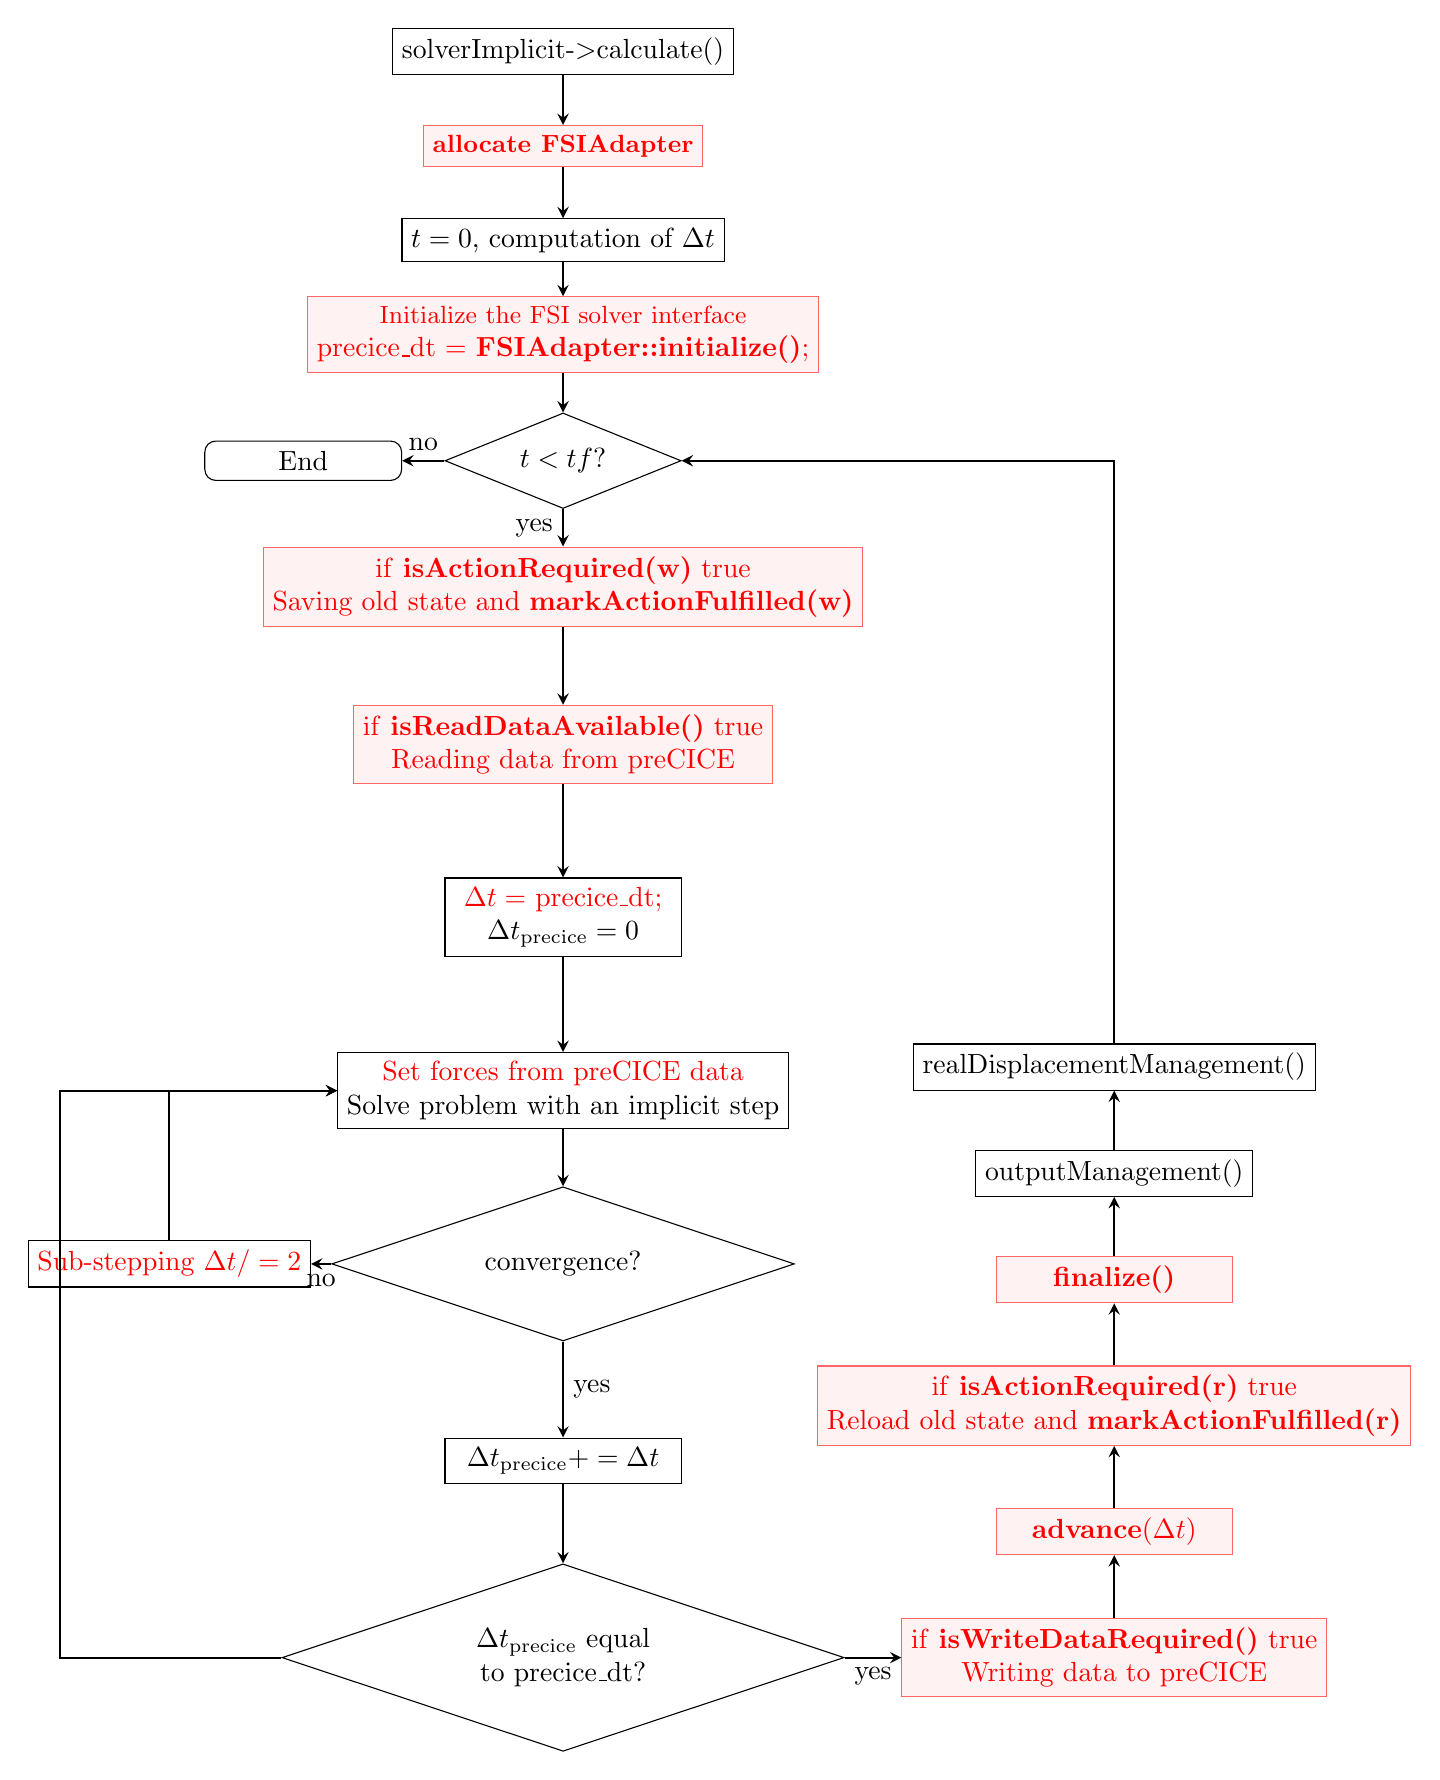
\begin{tikzpicture}[node distance=2cm]
	\node (start) [block] {solverImplicit-$>$calculate()};
	\node (blo1) [block, below of=start, yshift=+0.8cm, align=center, color=red!60, fill=red!5] {\color{red}\small\textbf{allocate FSIAdapter}};
	\node (blo2) [block, below of=blo1, yshift=+0.8cm] {$t=0$, computation of $\Delta t$};
	\node (blo3) [block, below of=blo2, yshift=+0.8cm, align=center, color=red!60, fill=red!5] {\color{red}\small Initialize the FSI solver interface\\\color{red}precice\_dt = \textbf{FSIAdapter::initialize()};};
	\node (dec1) [choix, below of=blo3, aspect=2, yshift=+0.4cm] {$t<tf$?};
	\node (blo4) [block, below of=dec1, yshift=+0.4cm, align=center, color=red!60, fill=red!5] {\color{red}if \textbf{isActionRequired(w)} true\\\color{red}Saving old state and \textbf{markActionFulfilled(w)}};
	\node (blo5) [block, below of=blo4, yshift=+0.cm, align=center, color=red!60, fill=red!5] {\color{red}if \textbf{isReadDataAvailable()} true\\\color{red}Reading data from preCICE};
	\node (blo6) [block, below of=blo5, yshift=-0.2cm, align=center] {\color{red}$\Delta t = $  precice\_dt;\\$\Delta t_\text{precice}=0$};
	\node (stop1) [terminus, left of=dec1, xshift=-1.3cm] {End};
	\node (blo7) [block, below of=blo6, yshift=-0.2cm,align=center] {\color{red}Set forces from preCICE data\\Solve problem with an implicit step};
	\node (dec2) [choix2, below of=blo7, aspect=3, yshift=-0.2cm] {convergence?};
	\node (blo71) [block, below of=dec2, yshift=-0.5cm,align=center]  {$\Delta t_\text{precice}+=\Delta t$};
	\node (dec3) [choix2, below of=blo71, aspect=3, yshift=-0.5cm] {$\Delta t_\text{precice}$ equal to precice\_dt?};
	\node (blo8) [block, right of=dec3, xshift=+5cm, align=center, color=red!60, fill=red!5] {\color{red}if \textbf{isWriteDataRequired()} true\\\color{red}Writing data to preCICE};
	\node (blo9) [block, above of=blo8, yshift=-0.4cm, color=red!60, fill=red!5] {\color{red}\textbf{advance}($\Delta t$)};
	\node (blo10) [block, above of=blo9, yshift=-0.4cm, align=center, color=red!60, fill=red!5] {\color{red}if \textbf{isActionRequired(r)} true\\\color{red}Reload old state and \textbf{markActionFulfilled(r)}};
	\node (blo22) [block, above of=blo10, yshift=-0.4cm, color=red!60, fill=red!5] {\color{red} \textbf{finalize()}};
	\node (blo11) [block, above of=blo22, yshift=-0.65cm] {outputManagement()};
	\node (blo12) [block, above of=blo11, yshift=-0.65cm] {realDisplacementManagement()};
	\node (blo13) [block, left of=dec2, xshift=-3cm] {\color{red}Sub-stepping $\Delta t/=2$};

	\draw [arrow] (start) -- (blo1);
	\draw [arrow] (blo1) -- (blo2);
	\draw [arrow] (blo2) -- (blo3);
	\draw [arrow] (blo3) -- (dec1);
	\draw [arrow] (dec1) -- node[anchor=south] {no} (stop1);
	\draw [arrow] (dec1) -- node[anchor=east] {yes} (blo4);
	\draw [arrow] (blo4) -- (blo5);
	\draw [arrow] (blo5) -- (blo6);
	\draw [arrow] (blo6) -- (blo7);
	\draw [arrow] (blo7) -- (dec2);
	\draw [arrow] (dec2) -- node[anchor=north] {no}(blo13);
	\draw [arrow] (dec2) -- node[anchor=west] {yes}(blo71);
	\draw [arrow] (blo71) --(dec3);
	\draw [arrow] (dec3) -- node[anchor=north] {yes} (blo8);
	\draw [arrow] (dec3.west) |- ++(-80pt,-0pt) |-  (blo7.west);
	\draw [arrow] (blo8) -- (blo9);
	\draw [arrow] (blo9) -- (blo10);
	\draw [arrow] (blo10) -- (blo22);
	\draw [arrow] (blo22) -- (blo11);
	\draw [arrow] (blo11) -- (blo12);
	\draw [arrow] (blo12.north) |- (dec1.east);
	\draw [arrow] (blo13) |- (blo7);
	\end{tikzpicture}
	\caption{Simplified structure of MuPhiSim Implicit Dynamic Solver with the addition of FSI options}
	\label{fig:solverIDFSI}
\end{figure}

If an FSI simulation is needed by the user, they should add to the input file the keyword \textbf{*FSI} followed by the list of nodes at the coupling interface by means of the corresponding label in the full list of nodes.\\

\subsection{OpenFOAM adapter}
For linking OpenFOAM and preCICE, an open-source adapter has been developed and can be downloaded from the preCICE website. However, to use it properly, some steps must be followed :
\begin{itemize}
    \item Write a \texttt{system/preciceDict}
    \item Set compatible boundary conditions
    \item Activate the adapter in \texttt{system/controlDict}.
\end{itemize}

The tree of the folder corresponding to the fluid part is shown in Figure \ref{arborescence}.

\begin{figure}[H]
    \centering
    \includegraphics[width=7cm]{imgs/Illustrations/arborescence.png}
    \caption{Tree of the \texttt{fluid-openfoam} folder\\ \emph{All the files participate in the configuration of the OpenFOAM adapter except the files clean.sh and run.sh which respectively cleans the folder and runs the simulation for the fluid.}}
    \label{arborescence}
\end{figure}

\texttt{preciceDict} is an OpenFOAM dictionary and the adapter’s configuration file. A list of the names of the OpenFOAM boundary patches that are participating in the coupled simulation is specified in this file. These need also to be defined in the files included in the \texttt{0/} directory.\\

The boundary conditions for the interface are set in the \texttt{0/} folder and the type of solver is specified in \texttt{constant/dynamicMeshDict}.\\

To load the adapter, the \texttt{system/controlDict} configuration file must direct the solver to use the \textbf{preciceAdapterFunctionObject} function object. This function is part of the \textbf{libpreciceAdapterFunctionObject.so} shared library, available with the OpenFOAM adapter.\\

Please refer to \textbf{https://precice.org/adapter-openfoam-config.html} to get all the configuration details.

\subsection{The role of preCICE}
Once the links between preCICE and the two solvers are established, all that remains is to configure the coupling algorithm so that the FSI simulation can be done.

\subsubsection{Configuration file}
Before launching a coupling simulation, preCICE must be configured at runtime via an .xml file named \texttt{precice-config.xml}. This file defines all coupling simulation choices made by the user.\\

\begin{figure}[H]
    \centering
    \includegraphics[width=14cm]{imgs/Illustrations/precice-config.png}
    \caption{Diagram of the coupled solvers\\ \texttt{precice-config.xml} \emph{configurates preCICE, which is represented by the green blocks.}}
    \label{configfile}
\end{figure}

The easiest way to write a configuration file is to use those given in the examples in either in the \textbf{quickstart} or \textbf{perpendicular\_flap} folders or in the preCICE tutorials.\\


First, the dimensions of the coupling simulation is set : \texttt{<solver-interface dimensions="2">}. This value agrees with the physical dimension of the simulation, i.e. the number of coordinates forces and displacements vertex have. However, OpenFOAM only supports 3D simulation and MuPhiSim is used in 2D. Hence, the OpenFOAM adapter maps from 3D to 2D as the \texttt{precice-config.xml} sets the preCICE dimension to 2D. As already mentioned, we recommend simulating mainly bidirectional problems as communication with preCICE is particularly expensive for volume coupled problems.\\


Then, the preCICE configuration file is structured in the following five sections :
\begin{itemize}
    \item \texttt{<data .../>}: defines the coupling data values the participants exchange. For the example case, these are displacements and forces. Once these fields are defined, MuPhiSim and OpenFOAM use the preCICE API to access them.
    \item \texttt{<mesh .../>}: defines the interface coupling meshes by giving them an ID transmitted to the solvers via the preCICE API.
    \item \texttt{<participant .../>}: the solvers that participate in the coupled simulation need a participant definition in the \texttt{xml} file. Each participant can either provide the mesh by defining the coordinates or receive the mesh coordinates from another participant who defines them. As the coordinates of the boundary nodes are defined in the MuPhiSim input file, it seems natural that the fluid participant should use the solid mesh. Thus, a data mapping is defined between both participants - see next section.
    \item \texttt{<m2n .../>}: defines a communication channel for the two participants to exchange data.
    \item \texttt{<coupling-scheme .../>}: where the two participants exchange data, the simulation time, the coupling scheme wanted, the coupling time window length (i.e. the coupling time step) are defined.
\end{itemize}

preCICE provides a tool to easily understand the \texttt{precic-config.xml} file with a simple shell command. This tool interprets the given configuration file and visualizes it as a graph, represented in Figure \ref{graph}. See at \textbf{https://precice.org/tooling-config-visualization.html} for further information.

\begin{figure}[h]
    \centering
    \includegraphics[width=14cm]{imgs/Illustrations/graph.pdf}
    \caption{Graph showing the configuration of preCICE for the example studied\\ \emph{This schematic view of the} \texttt{precic-config.xml} \emph{file helps to understand how works the FSI simulation.}}
    \label{graph}
\end{figure}

\subsubsection{Mapping configuration}
The FSI simulation requires the communication of data from the coupling surface of the deformable body to the coupling surface of the fluid. Thus, coupling the two participants at a common interface generally means mapping data between surface meshes which do not match. To deal with this issue, preCICE provides a choice of data mapping methods to map coupling data from one mesh to the other [12,13]. Each coupled variable can be mapped in either consistent or conservative form.\\

As part of its black box approach, preCICE only uses nodal values, values at mesh vertices. Consider two meshes, a fine and a coarse grid. If the value at coarse nodes is the same as the value at the corresponding fine node, the type of the mapping is consistent. A consistent mapping exactly reproduces constant functions at the coupling surface. It is usually applied to values such as densities and fluxes. In the case studied, the displacement data is mapped in a consistent form.\\

Conservative mappings preserve integral values. The value at a coarse node is computed as a sum of the corresponding fine nodes, such that the total coupling value on the coarse and fine mesh is the same. This type of mapping is applied to forces in the example case.\\

preCICE provides three mapping methods :
\begin{itemize}
    \item Nearest-Neighbor mapping is a first-order method that only requires vertex position information and works locally. As represented in Figure \ref{mapping}, a data point in the target mesh is assigned the value of the data point in the source mesh that is the closest to its position.
\begin{figure}[H]
    \centering
    \includegraphics[width=14cm]{imgs/Illustrations/mapping.png}
    \caption{Nearest-Neighbor and Nearest-Projection mappings\\ \emph{These two mapping configuration are different ways to exchange date between a source and a target mesh.}}
    \label{mapping}
\end{figure}
    \item Nearest-Projection mapping is a second-order method based on projections of data points of the target mesh to mesh elements of the source mesh and a linear interpolation scheme in these elements. This method is relatively fast and numerically superior to nearest-neighbor. However, using this method requires mesh connectivity information to be defined.
    \item Radial Basis Function (RBF) mapping is a method that requires no topological information and works well on general non-matching meshes. This mapping uses radially-symmetric basis functions centered on each vertex of the source mesh. Many choices for the basis functions are implemented in preCICE and are listed in [13].
\end{itemize}

For the coupling simulation studied, the radial basis function has been used with a \texttt{thin-plate-splines} type. Indeed, as nearest-projection, radial basis function mapping behaves as a second-order method, but without the need to define mesh connectivity information. Moreover, basis function with global support are easier to configure as only a few parameters need to be set.

\subsubsection{Communication}
Communication between participants works point-to-point [12,13]. preCICE analyses the mesh decomposition of both participants and constructs only local communication channels when needed. Therefore, mesh connectivity is often not necessary: a cloud of vertices as coupling mesh is sufficient for most of the numerical methods that preCICE offers.

\subsubsection{Coupling schemes: explicit/implicit and serial/parallel}
One of the main assets of preCICE is its adaptability to different schemes. Indeed, preCICE offers a variety of coupling schemes : either serial or parallel and either explicit or implicit.\\

The user can chose whether to run a serial or a parallel coupling scheme. With a serial scheme, the participants run after one another while with a parallel one the participants run simultaneously. Nothing needs to be changed in the solver code to switch from a serial to a parallel coupling scheme thanks to the high-level API of preCICE.\\

It is also possible to choose between an explicit and an implicit scheme [13].
Denote $x$ as the forces data and $y$ the displacements data so that
\begin{equation}
    \left\{
        \begin{array}{r c l}
        S_1 : x \rightarrow y\\
        S_2 : y \rightarrow x
        \end{array}
        \right.
\end{equation}
where $S_1$ and $S_2$ are respectively the mappings of MuPhiSim and OpenFOAM routines.\\

With an explicit scheme, both participants are only executed once per time window. Used with the serial scheme, the system to solve at every time step is the following :
\begin{equation}
    \left\{
        \begin{array}{r c l}
        S_1^n(x^n) = y^{n+1}\\
        S_2^n(y^{n+1}) = x^{n+1}
        \end{array}
        \right.
\end{equation}
However, this implies a staggered execution of the two solvers. The parallel scheme avoids this by using old time step values $x^n$ and $y^n$ as an input for both solvers :
\begin{equation}
    \left\{
        \begin{array}{r c l}
        S_1^n(x^n) = y^{n+1}\\
        S_2^n(y^n) = x^{n+1}
        \end{array}
        \right.
\end{equation}

Implicit coupling schemes iterate over a coupling equation until convergence. This means that the participants are coupled iteratively, repeating each coupling time window until both solvers have converged to the same values. With a serial scheme, the following system is solved for each iteration $i$ :
\begin{equation}
    \left\{
        \begin{array}{r c l}
        S_1^n(x^{n+1}_i) = y^{n+1}_{i+1}\\
        S_2^n(y^{n+1}_{i+1}) = x^{n+1}_{i+1}
        \end{array}
        \right.
\end{equation}
whereas a parallel scheme computes the new values for a given iteration $x^{n+1}$ and $y^{n+1}$ simultaneously :
\begin{equation}
    \left\{
        \begin{array}{r c l}
        S_1^n(x^{n+1}_i) = y^{n+1}_{i+1}\\
        S_2^n(y^{n+1}_{i}) = x^{n+1}_{i+1}
        \end{array}
        \right.
\end{equation}

The iterations of implicit coupling schemes can be reduced by using acceleration techniques that allow the data exchanged to be modified by preCICE. Three different types of acceleration are provided: constant (constant under-relaxation), aitken (adaptive under-relaxation), and various quasi-Newton variants (IQN-ILS aka. Anderson acceleration, IQN-IMVJ aka. generalized Broyden) [12,13]. The acceleration modifies coupling data in advance() to stabilize values by using a linear combination of values from previous iterations. For the case studied, the Anderson acceleration is used as the Quasi-Newton acceleration is recommended for strong interactions.

\textbf{IMPORTANT : Once the \texttt{precic-config.xml} file has been edited, the path to the preCICE configuration file in the FSI configuration settings must be specified in the \textbf{solverImplicit.cpp} file !}

\section{Example}


Consider a deformable body in a fluid flow inside a channel. The diagram of this example can be seen in Figure 13.3. The flap is fixed at a rotation point, constituting Dirichlet boundary conditions. The structure has a density of $\rho_s = 1.0.10^4 kg.m^{-3}$, the Poisson ratio $\nu = 0.3$ and a Young's modulus of $1.0.10^6 kg.m^{-1}.s^{-2}$. The simulation time was set at 2.5 seconds.  This is a bidirectional surface coupling. Indeed, communication with preCICE is particularly expensive for volume coupled problems [13].\\

\begin{figure}[h]
    \centering
    \includegraphics[width=15cm]{imgs/Illustrations/example.png}
    \caption{Diagram of the case study\\ \emph{The simple example studied is a deformable body in a fluid flow inside a channel. The flap is fixed at a rotation point.}}
    \label{}
\end{figure}

For this example, only FEM nodes and elements are defined. The material keyword used is \textbf{*HyperElastic, St-Venant-Kirchhoff}. This is equivalent to linear elastic for small deformation. The type of solver used was \textbf{IMPLICIT} (dynamic).\\

Returning to the example, the angle of attack of the flow must be sufficient to set the solid in motion. This is ensured by the point of rotation being set in the upper left corner of the flap. Boundary conditions were defined in the input file before running the simulation.\\

preCICE follows a peer-to-peer approach: in order to run a simulation, the user have to start the coupled solvers individually in two different terminals.

Paraview allows the fluid and solid results to be viewed either together or separately. Results can be shown in Figure \ref{result1} and \ref{result2}.
\begin{figure}[H]
    \centering
    \includegraphics[width=15cm]{imgs/Illustrations/result flap.png}
    \caption{Result of the FSI simulation for the deformable solid (screenshot of the Paraview window)\\ \emph{This screenshot represents the $50^{th}$ MuPhiSim output file, corresponding to a time simulation of $0.0619377\,s$}}
    \label{result1}
\end{figure}
Paraview provides to the user several filters to visualize the results properly. Here, The ``Glyph'' and ``WrapByVector'' filters have been used. The former displays the displacements with arrows and the latter enables to deform the coupling data.\\
\begin{figure}[h]
    \centering
    \includegraphics[width=15cm]{imgs/Illustrations/result both.png}
    \caption{Result of the FSI simulation (screenshot of the Paraview window)\\ \emph{This screenshot corresponds to a time simulation of $0.15\,s$ }}
    \label{result2}
\end{figure}


%%%%%%%%%%%%%%%%%%%%%%%%%%%%%%%%%%%%%%% CHAPTER 14
%%%%%%%%%%%%%%%%%%%%%%%%%%%%%%%%%%%%%%%%%%%%
%%\chapter{Acknowledgements and Credits}

%%This manual was created by S.Bielle by merging the works of many engineers who worked at different levels of \textit{MuPhiSim}. I would like to thank Profs. Antoine J\'{e}rusalem and Charlotte Kirchhelle for their support and their availability along the months I worked on \textit{MuPhiSim} and also, Aaron Graham for the correction of grammar errors.
%%}

%%%%%%%%%%%%%%%%%%%%%%%%%%%%%%%%%%%%%%%% APPENDIX %%%%%%%%%%%%%%%%%%%%%%%%%%%%%%%%%%%%%%%%%%%%
\appendix
\chapter[APPENDIX A]{ACTIVATION/DEACTIVATION OF ELEMENTS}
This chapter includes the element progressive activation/deactivation capabilities in MuPhiSim. Typical examples include analysing  fracture and additive manufacturing.

To use activation/deactivation option, the input file must to include the keyword \textbf{*ACTIVATION} just after the line that specific the analysis type. All the elements will be defined as active by default. The activation status occurs at the beginning of a load step. The different criteria for activation/deactivation must be defined in the constitutive model (the criteria can be defined in the mechanical or extraDof models; however, this status will affect all the DOF, not just the ones used in that specific model). Note that elements cannot be partially activated. This means that the status of the element can change only from inactive to fully active. That provides a stepped change in the element status. Following this premise, boundary conditions have to be defined as instantaneous.

Unlike other FEM software, where the stiffness matrix and load vectors size is always preserved, in order to decrease the computational cost, the stiffness matrix, residual and deltaU vectors change according with the active DOF (not including Dirichlet DOF) in each step.

\chapter[APPENDIX C]{Tangent modulus of the Neo-Hookean constitutive model}
Considering a material that follows a Neo-Hookean constitutive law, the expression of the first Piola-Kirchhoff stress is :

\begin{equation}
    P = \frac{\mu}{J^{\frac{2}{3}}}(F - \frac{1}{3}trace(B)F^{-T}) +K_{1}J(J-1)F^{-T}
    \end{equation}
The expression of the tangent modulus by taking the derivative of P with respect to F is derived by:

\begin{equation}
\begin{split}
\frac{\partial P}{\partial F} = \mu(F\otimes\frac{\partial(J^{\frac{-2}{ndim}})}{\partial F} + J^{\frac{2}{ndim}}\frac{\partial F}{\partial F} -  \frac{1}{ndim}(F^{-T}\otimes \frac{\partial trace(B)}{\partial F} +\\
trace(B)\frac{\partial F^{-T}}{\partial F}) +
K_{1}(F^{-T}\otimes\frac{\partial J(J-1)}{\partial F}+J(J-1)\frac{\partial F^{-T}}{\partial F}).
\end{split}
\end{equation}

After all calculation are done, one obtains:

\begin{equation}
\begin{split}
C_{iJkL} = \frac{\mu}{J^{\frac{2}{ndim}}}(\delta_{iK}\delta_{Jl}
-\frac{2}{ndim}F_{Lk}^{-1}F_{iJ}+\frac{1}{ndim}traceB(F_{Li}^{-1}F_{Jk}^{-1})+ \\
\frac{-1}{ndim}(\frac{-2}{ndim}F_{Lk}^{-1}trace(B)+F_{kL}F_{Ji}^{-1})) +K_{1}J(J-1)(-F_{Li}^{-1}F_{Jk}^{-1})+(2J^{2}-J)(F_{Lk}^{-1}F_{Ji}^{-1}).
\end{split}
\end{equation}


%%%%%%%%%%%%%%%%%%%%%%%%%%%%%%%%%%%%%%%% BIBLIO %%%%%%%%%%%%%%%%%%%%%%%%%%%%%%%%%%%%%%%%%%%%
\bibliographystyle{apalike}%{apalike}
\bibliography{biblio}


[11] "About OpenFOAM", \emph{OpenFOAM}, https://www.openfoam.com/. Accessed Aug. 2021.\\

[12] "The preCICE documentation", \emph{preCICE - The Coupling Library},\\ https://precice.org/docs.html. Accessed Aug. 2021.\\

[13] Hans-Joachim Bungartz, Florian Lindner, Bernhard Gatzhammer, Miriam Mehl, Klaudius Scheufele, Alexander Shukaev, Benjamin Uekermann, \emph{preCICE – A fully parallel library for multi-physics surface coupling}, Computers \& Fluids, Volume 141, 2016, Pages 250-258, ISSN 0045-7930, \\https://doi.org/10.1016/j.compfluid.2016.04.003.\\

[14] David Schneider, "Material when writing about preCICE", \emph{precice.github.io/material/},\\ https://github.com/precice/precice.github.io/tree/master/material. Accessed Aug. 2021.\\

[15] Gerasimos Chourdakis,  \emph{A general OpenFOAM adapter for the coupling library preCICE}, Master's thesis, Department of Informatics, Technical University of Munich, 2017.\\
\end{document}
